\documentclass[../main.tex]{subfiles}

\begin{document}
    \subsubsection*{Uncertainties}
        Every following uncertainty was calculated using this formula
        \[u:=\fdef{\fdef{\sqrt{\sum_{i\in\text{Def}(x)}\diff{f}{u(x_i)}{x}{}}}{x\in\text{Def}{f}}}{f\in C^(\R^d,\R)}.\]
		        
        
    \subsection{Isentropric Exponent}
        \subsubsection*{Measurement according to Rüchhardt and Flammersfed}
            The measurements as described in \ref{sec:RuchhartFlammersfeld} yielded the following results for the isentropic exponent:

            \begin{table}[H]
                \centering
                \begin{tabular}{c|c|c}
                    \textbf{Gas} & \textbf{Oscillation period in s} & \textbf{Isentropic exponent}\\
                    \hline
                    $\text{Ar}$ & $0.9040(31)$ & $1.808$\\
                    $\text{CO}_2$ & $1.2050(31)$ & $1.406$\\
                    $\text{N}_2$ & $1.266(67)$ & $0.921$\\
                \end{tabular}
                \caption{isentropic exponents for different gases. The oscillation period refers to the oscillation period of the small metal cylinder. No Uncertainties are given because of their neglible size}
                \label{fig:KappaRuchhardtFlammersfeld}
            \end{table}

            \noindent Compared to the literature values of $\kappa_{\text{Ar}}=1.648$, $\kappa_{\text{N}_2}=1.401$, $\kappa_{\text{CO}_2}=1.293$, the obtain values are close but not compatible \cite[p.258]{skript}. One cause for this are the small used uncertainties. Thus, there may be some larger uncertainties yet to be accounted for.

        \subsubsection*{Clément and Desormes}
            Following the experiment described by Clément and Desormes \ref{sec:ClementDesormes}, we obtained the values for $\kappa$ depicted below:
            
            \begin{table}[H]
                \centering
                \begin{tabular}{c|cc|c}
                    \textbf{Gas} & \textbf{Height $h_1$ in cm} & \textbf{Height $h_1$ in cm} & \textbf{Isentropic exponent}\\
                    \hline
                    $\text{Ar}$ & $9.46(30)$ & $7.16(30)$ & $4.12(46)$\\
                    $\text{CO}_2$ & $10.26(30)$ & $7.26(30)$ & $3.42(18)$\\
                    $\text{N}_2$ & $9.86(30)$ & $7.29(30)$ & $3.84(32)$\\
                \end{tabular}
                \caption{isentropic exponents for different gases. $h_1$ and $h_3$ are the heights of the water pillar before and after the pressure release of the gas}
            \end{table}
            
            These measurements for $\kappa$ are almoust twice as much as the literature values or the ones in \ref{fig:KappaRuchhardtFlammersfeld}. One possible explanation is during the experiment, small air bubbles formed inside the water pillars, which might have rendered the formula connection $h_1,h_3$ and pressure differences inaccurate.

    \subsection{Degrees of freedom}
        We firstly deduce the following plots from our data. 
        % \begin{figure}[H]

	\centering
	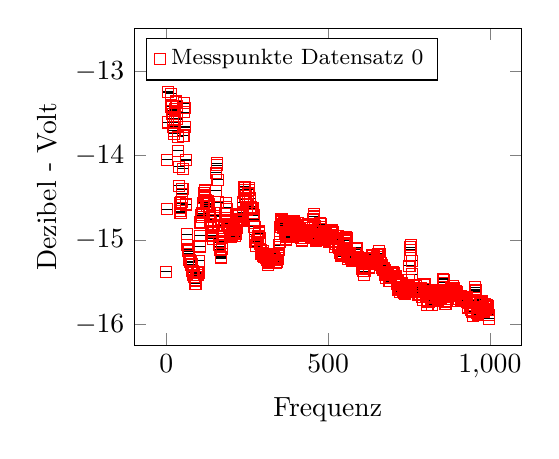
\begin{tikzpicture}
		\pgfplotsset{width=6.5cm,compat=1.3,legend style={font=\footnotesize}}
		\begin{axis}[xlabel={Frequenz},ylabel={Dezibel - Volt},legend cell align=left,legend pos=north west]
		
\addplot+[only marks,color=red,mark=square,error bars/.cd,x dir=both,x explicit,y dir=both,y explicit,error bar style={color=black}] table[x=X,y=Y,x error=xerror,y error=yerror,row sep=\\]{
			X	Y	xerror	yerror	\\
			 0.0 	 -15.377863 	 0 	 0 	\\
			 1.464844 	 -14.634824 	 0 	 0 	\\
			 2.929687 	 -14.048924 	 0 	 0 	\\
			 4.394531 	 -13.606714 	 0 	 0 	\\
			 5.859375 	 -13.245078 	 0 	 0 	\\
			 7.324219 	 -12.971722 	 0 	 0 	\\
			 8.789062 	 -12.828342 	 0 	 0 	\\
			 10.253906 	 -12.80232 	 0 	 0 	\\
			 11.71875 	 -12.891995 	 0 	 0 	\\
			 13.183594 	 -13.047378 	 0 	 0 	\\
			 14.648437 	 -13.266726 	 0 	 0 	\\
			 16.113281 	 -13.417296 	 0 	 0 	\\
			 17.578125 	 -13.467953 	 0 	 0 	\\
			 19.042969 	 -13.510851 	 0 	 0 	\\
			 20.507812 	 -13.562329 	 0 	 0 	\\
			 21.972656 	 -13.65778 	 0 	 0 	\\
			 23.4375 	 -13.742413 	 0 	 0 	\\
			 24.902344 	 -13.70612 	 0 	 0 	\\
			 26.367187 	 -13.603597 	 0 	 0 	\\
			 27.832031 	 -13.452496 	 0 	 0 	\\
			 29.296875 	 -13.360224 	 0 	 0 	\\
			 30.761719 	 -13.347933 	 0 	 0 	\\
			 32.226562 	 -13.416004 	 0 	 0 	\\
			 33.691406 	 -13.565305 	 0 	 0 	\\
			 35.15625 	 -13.777465 	 0 	 0 	\\
			 36.621094 	 -13.942297 	 0 	 0 	\\
			 38.085937 	 -14.13413 	 0 	 0 	\\
			 39.550781 	 -14.355808 	 0 	 0 	\\
			 41.015625 	 -14.567138 	 0 	 0 	\\
			 42.480469 	 -14.661787 	 0 	 0 	\\
			 43.945312 	 -14.676044 	 0 	 0 	\\
			 45.410156 	 -14.624667 	 0 	 0 	\\
			 46.875 	 -14.554264 	 0 	 0 	\\
			 48.339844 	 -14.454346 	 0 	 0 	\\
			 49.804687 	 -14.396066 	 0 	 0 	\\
			 51.269531 	 -14.157371 	 0 	 0 	\\
			 52.734375 	 -13.76188 	 0 	 0 	\\
			 54.199219 	 -13.486916 	 0 	 0 	\\
			 55.664062 	 -13.378995 	 0 	 0 	\\
			 57.128906 	 -13.436821 	 0 	 0 	\\
			 58.59375 	 -13.660917 	 0 	 0 	\\
			 60.058594 	 -14.051488 	 0 	 0 	\\
			 61.523437 	 -14.579972 	 0 	 0 	\\
			 62.988281 	 -14.932836 	 0 	 0 	\\
			 64.453125 	 -15.057708 	 0 	 0 	\\
			 65.917969 	 -15.10667 	 0 	 0 	\\
			 67.382812 	 -15.131666 	 0 	 0 	\\
			 68.847656 	 -15.120015 	 0 	 0 	\\
			 70.3125 	 -15.166563 	 0 	 0 	\\
			 71.777344 	 -15.234852 	 0 	 0 	\\
			 73.242187 	 -15.257725 	 0 	 0 	\\
			 74.707031 	 -15.258081 	 0 	 0 	\\
			 76.171875 	 -15.262162 	 0 	 0 	\\
			 77.636719 	 -15.292419 	 0 	 0 	\\
			 79.101562 	 -15.302074 	 0 	 0 	\\
			 80.566406 	 -15.371643 	 0 	 0 	\\
			 82.03125 	 -15.414623 	 0 	 0 	\\
			 83.496094 	 -15.384488 	 0 	 0 	\\
			 84.960937 	 -15.38654 	 0 	 0 	\\
			 86.425781 	 -15.435651 	 0 	 0 	\\
			 87.890625 	 -15.480934 	 0 	 0 	\\
			 89.355469 	 -15.519261 	 0 	 0 	\\
			 90.820312 	 -15.520492 	 0 	 0 	\\
			 92.285156 	 -15.435193 	 0 	 0 	\\
			 93.75 	 -15.419489 	 0 	 0 	\\
			 95.214844 	 -15.394684 	 0 	 0 	\\
			 96.679687 	 -15.392082 	 0 	 0 	\\
			 98.144531 	 -15.417509 	 0 	 0 	\\
			 99.609375 	 -15.390234 	 0 	 0 	\\
			 101.074219 	 -15.246798 	 0 	 0 	\\
			 102.539062 	 -15.077027 	 0 	 0 	\\
			 104.003906 	 -14.951796 	 0 	 0 	\\
			 105.46875 	 -14.793155 	 0 	 0 	\\
			 106.933594 	 -14.725076 	 0 	 0 	\\
			 108.398437 	 -14.70885 	 0 	 0 	\\
			 109.863281 	 -14.729992 	 0 	 0 	\\
			 111.328125 	 -14.683022 	 0 	 0 	\\
			 112.792969 	 -14.633574 	 0 	 0 	\\
			 114.257812 	 -14.559146 	 0 	 0 	\\
			 115.722656 	 -14.497235 	 0 	 0 	\\
			 117.1875 	 -14.442762 	 0 	 0 	\\
			 118.652344 	 -14.413613 	 0 	 0 	\\
			 120.117187 	 -14.473501 	 0 	 0 	\\
			 121.582031 	 -14.529763 	 0 	 0 	\\
			 123.046875 	 -14.572319 	 0 	 0 	\\
			 124.511719 	 -14.599137 	 0 	 0 	\\
			 125.976562 	 -14.57376 	 0 	 0 	\\
			 127.441406 	 -14.5452 	 0 	 0 	\\
			 128.90625 	 -14.577725 	 0 	 0 	\\
			 130.371094 	 -14.570568 	 0 	 0 	\\
			 131.835937 	 -14.606959 	 0 	 0 	\\
			 133.300781 	 -14.677834 	 0 	 0 	\\
			 134.765625 	 -14.72607 	 0 	 0 	\\
			 136.230469 	 -14.783752 	 0 	 0 	\\
			 137.695312 	 -14.845978 	 0 	 0 	\\
			 139.160156 	 -14.890022 	 0 	 0 	\\
			 140.625 	 -14.942508 	 0 	 0 	\\
			 142.089844 	 -14.958278 	 0 	 0 	\\
			 143.554687 	 -14.984087 	 0 	 0 	\\
			 145.019531 	 -14.907987 	 0 	 0 	\\
			 146.484375 	 -14.833804 	 0 	 0 	\\
			 147.949219 	 -14.760233 	 0 	 0 	\\
			 149.414062 	 -14.716789 	 0 	 0 	\\
			 150.878906 	 -14.612332 	 0 	 0 	\\
			 152.34375 	 -14.415131 	 0 	 0 	\\
			 153.808594 	 -14.203882 	 0 	 0 	\\
			 155.273437 	 -14.090973 	 0 	 0 	\\
			 156.738281 	 -14.114061 	 0 	 0 	\\
			 158.203125 	 -14.28813 	 0 	 0 	\\
			 159.667969 	 -14.549723 	 0 	 0 	\\
			 161.132812 	 -14.826476 	 0 	 0 	\\
			 162.597656 	 -15.024029 	 0 	 0 	\\
			 164.0625 	 -15.059548 	 0 	 0 	\\
			 165.527344 	 -15.076732 	 0 	 0 	\\
			 166.992187 	 -15.118956 	 0 	 0 	\\
			 168.457031 	 -15.214337 	 0 	 0 	\\
			 169.921875 	 -15.197879 	 0 	 0 	\\
			 171.386719 	 -15.102572 	 0 	 0 	\\
			 172.851562 	 -15.033952 	 0 	 0 	\\
			 174.316406 	 -14.968841 	 0 	 0 	\\
			 175.78125 	 -14.886593 	 0 	 0 	\\
			 177.246094 	 -14.857826 	 0 	 0 	\\
			 178.710937 	 -14.834681 	 0 	 0 	\\
			 180.175781 	 -14.781653 	 0 	 0 	\\
			 181.640625 	 -14.697632 	 0 	 0 	\\
			 183.105469 	 -14.612491 	 0 	 0 	\\
			 184.570312 	 -14.565412 	 0 	 0 	\\
			 186.035156 	 -14.630101 	 0 	 0 	\\
			 187.5 	 -14.763068 	 0 	 0 	\\
			 188.964844 	 -14.81181 	 0 	 0 	\\
			 190.429687 	 -14.809167 	 0 	 0 	\\
			 191.894531 	 -14.820498 	 0 	 0 	\\
			 193.359375 	 -14.83837 	 0 	 0 	\\
			 194.824219 	 -14.842676 	 0 	 0 	\\
			 196.289062 	 -14.914527 	 0 	 0 	\\
			 197.753906 	 -14.937226 	 0 	 0 	\\
			 199.21875 	 -14.963659 	 0 	 0 	\\
			 200.683594 	 -14.964335 	 0 	 0 	\\
			 202.148437 	 -14.949748 	 0 	 0 	\\
			 203.613281 	 -14.918795 	 0 	 0 	\\
			 205.078125 	 -14.910389 	 0 	 0 	\\
			 206.542969 	 -14.885805 	 0 	 0 	\\
			 208.007812 	 -14.866659 	 0 	 0 	\\
			 209.472656 	 -14.877181 	 0 	 0 	\\
			 210.9375 	 -14.919722 	 0 	 0 	\\
			 212.402344 	 -14.957385 	 0 	 0 	\\
			 213.867187 	 -14.929474 	 0 	 0 	\\
			 215.332031 	 -14.902048 	 0 	 0 	\\
			 216.796875 	 -14.855239 	 0 	 0 	\\
			 218.261719 	 -14.814927 	 0 	 0 	\\
			 219.726562 	 -14.754177 	 0 	 0 	\\
			 221.191406 	 -14.698331 	 0 	 0 	\\
			 222.65625 	 -14.7121 	 0 	 0 	\\
			 224.121094 	 -14.720584 	 0 	 0 	\\
			 225.585937 	 -14.752912 	 0 	 0 	\\
			 227.050781 	 -14.754292 	 0 	 0 	\\
			 228.515625 	 -14.7607 	 0 	 0 	\\
			 229.980469 	 -14.754367 	 0 	 0 	\\
			 231.445312 	 -14.766731 	 0 	 0 	\\
			 232.910156 	 -14.774063 	 0 	 0 	\\
			 234.375 	 -14.75994 	 0 	 0 	\\
			 235.839844 	 -14.672699 	 0 	 0 	\\
			 237.304687 	 -14.553177 	 0 	 0 	\\
			 238.769531 	 -14.442574 	 0 	 0 	\\
			 240.234375 	 -14.380149 	 0 	 0 	\\
			 241.699219 	 -14.37053 	 0 	 0 	\\
			 243.164062 	 -14.405877 	 0 	 0 	\\
			 244.628906 	 -14.478126 	 0 	 0 	\\
			 246.09375 	 -14.525214 	 0 	 0 	\\
			 247.558594 	 -14.571617 	 0 	 0 	\\
			 249.023437 	 -14.640223 	 0 	 0 	\\
			 250.488281 	 -14.62722 	 0 	 0 	\\
			 251.953125 	 -14.545152 	 0 	 0 	\\
			 253.417969 	 -14.450371 	 0 	 0 	\\
			 254.882812 	 -14.385941 	 0 	 0 	\\
			 256.347656 	 -14.403229 	 0 	 0 	\\
			 257.8125 	 -14.507634 	 0 	 0 	\\
			 259.277344 	 -14.623046 	 0 	 0 	\\
			 260.742187 	 -14.619449 	 0 	 0 	\\
			 262.207031 	 -14.607496 	 0 	 0 	\\
			 263.671875 	 -14.6373 	 0 	 0 	\\
			 265.136719 	 -14.621309 	 0 	 0 	\\
			 266.601562 	 -14.623232 	 0 	 0 	\\
			 268.066406 	 -14.675993 	 0 	 0 	\\
			 269.53125 	 -14.705281 	 0 	 0 	\\
			 270.996094 	 -14.7643 	 0 	 0 	\\
			 272.460937 	 -14.844184 	 0 	 0 	\\
			 273.925781 	 -14.933865 	 0 	 0 	\\
			 275.390625 	 -15.023675 	 0 	 0 	\\
			 276.855469 	 -15.074193 	 0 	 0 	\\
			 278.320312 	 -15.070534 	 0 	 0 	\\
			 279.785156 	 -15.020149 	 0 	 0 	\\
			 281.25 	 -14.997145 	 0 	 0 	\\
			 282.714844 	 -14.974335 	 0 	 0 	\\
			 284.179687 	 -14.95966 	 0 	 0 	\\
			 285.644531 	 -14.900165 	 0 	 0 	\\
			 287.109375 	 -14.919175 	 0 	 0 	\\
			 288.574219 	 -14.978309 	 0 	 0 	\\
			 290.039062 	 -15.051671 	 0 	 0 	\\
			 291.503906 	 -15.121433 	 0 	 0 	\\
			 292.96875 	 -15.166601 	 0 	 0 	\\
			 294.433594 	 -15.162406 	 0 	 0 	\\
			 295.898437 	 -15.158841 	 0 	 0 	\\
			 297.363281 	 -15.136656 	 0 	 0 	\\
			 298.828125 	 -15.155136 	 0 	 0 	\\
			 300.292969 	 -15.186434 	 0 	 0 	\\
			 301.757812 	 -15.204195 	 0 	 0 	\\
			 303.222656 	 -15.177276 	 0 	 0 	\\
			 304.6875 	 -15.183911 	 0 	 0 	\\
			 306.152344 	 -15.169498 	 0 	 0 	\\
			 307.617187 	 -15.183561 	 0 	 0 	\\
			 309.082031 	 -15.208333 	 0 	 0 	\\
			 310.546875 	 -15.236216 	 0 	 0 	\\
			 312.011719 	 -15.223957 	 0 	 0 	\\
			 313.476562 	 -15.265625 	 0 	 0 	\\
			 314.941406 	 -15.293078 	 0 	 0 	\\
			 316.40625 	 -15.269928 	 0 	 0 	\\
			 317.871094 	 -15.246589 	 0 	 0 	\\
			 319.335937 	 -15.235773 	 0 	 0 	\\
			 320.800781 	 -15.236421 	 0 	 0 	\\
			 322.265625 	 -15.202186 	 0 	 0 	\\
			 323.730469 	 -15.174848 	 0 	 0 	\\
			 325.195312 	 -15.166102 	 0 	 0 	\\
			 326.660156 	 -15.188197 	 0 	 0 	\\
			 328.125 	 -15.181395 	 0 	 0 	\\
			 329.589844 	 -15.162683 	 0 	 0 	\\
			 331.054687 	 -15.166449 	 0 	 0 	\\
			 332.519531 	 -15.196976 	 0 	 0 	\\
			 333.984375 	 -15.217628 	 0 	 0 	\\
			 335.449219 	 -15.211973 	 0 	 0 	\\
			 336.914062 	 -15.242704 	 0 	 0 	\\
			 338.378906 	 -15.267842 	 0 	 0 	\\
			 339.84375 	 -15.270764 	 0 	 0 	\\
			 341.308594 	 -15.259543 	 0 	 0 	\\
			 342.773437 	 -15.233829 	 0 	 0 	\\
			 344.238281 	 -15.219391 	 0 	 0 	\\
			 345.703125 	 -15.173472 	 0 	 0 	\\
			 347.167969 	 -15.116821 	 0 	 0 	\\
			 348.632812 	 -15.060204 	 0 	 0 	\\
			 350.097656 	 -15.020687 	 0 	 0 	\\
			 351.5625 	 -14.95811 	 0 	 0 	\\
			 353.027344 	 -14.843255 	 0 	 0 	\\
			 354.492187 	 -14.770459 	 0 	 0 	\\
			 355.957031 	 -14.749877 	 0 	 0 	\\
			 357.421875 	 -14.790935 	 0 	 0 	\\
			 358.886719 	 -14.815091 	 0 	 0 	\\
			 360.351562 	 -14.829277 	 0 	 0 	\\
			 361.816406 	 -14.859088 	 0 	 0 	\\
			 363.28125 	 -14.840884 	 0 	 0 	\\
			 364.746094 	 -14.800479 	 0 	 0 	\\
			 366.210937 	 -14.83119 	 0 	 0 	\\
			 367.675781 	 -14.922398 	 0 	 0 	\\
			 369.140625 	 -14.984439 	 0 	 0 	\\
			 370.605469 	 -15.002639 	 0 	 0 	\\
			 372.070312 	 -14.9656 	 0 	 0 	\\
			 373.535156 	 -14.9294 	 0 	 0 	\\
			 375.0 	 -14.915619 	 0 	 0 	\\
			 376.464844 	 -14.935517 	 0 	 0 	\\
			 377.929687 	 -14.91687 	 0 	 0 	\\
			 379.394531 	 -14.875338 	 0 	 0 	\\
			 380.859375 	 -14.886914 	 0 	 0 	\\
			 382.324219 	 -14.926704 	 0 	 0 	\\
			 383.789062 	 -14.958619 	 0 	 0 	\\
			 385.253906 	 -14.929833 	 0 	 0 	\\
			 386.71875 	 -14.858562 	 0 	 0 	\\
			 388.183594 	 -14.86051 	 0 	 0 	\\
			 389.648437 	 -14.830076 	 0 	 0 	\\
			 391.113281 	 -14.821938 	 0 	 0 	\\
			 392.578125 	 -14.818603 	 0 	 0 	\\
			 394.042969 	 -14.787719 	 0 	 0 	\\
			 395.507812 	 -14.77604 	 0 	 0 	\\
			 396.972656 	 -14.806179 	 0 	 0 	\\
			 398.4375 	 -14.859224 	 0 	 0 	\\
			 399.902344 	 -14.943791 	 0 	 0 	\\
			 401.367187 	 -14.912992 	 0 	 0 	\\
			 402.832031 	 -14.871232 	 0 	 0 	\\
			 404.296875 	 -14.852966 	 0 	 0 	\\
			 405.761719 	 -14.800711 	 0 	 0 	\\
			 407.226562 	 -14.830097 	 0 	 0 	\\
			 408.691406 	 -14.862748 	 0 	 0 	\\
			 410.15625 	 -14.903424 	 0 	 0 	\\
			 411.621094 	 -14.881023 	 0 	 0 	\\
			 413.085937 	 -14.860914 	 0 	 0 	\\
			 414.550781 	 -14.886766 	 0 	 0 	\\
			 416.015625 	 -14.925458 	 0 	 0 	\\
			 417.480469 	 -14.982026 	 0 	 0 	\\
			 418.945312 	 -14.996119 	 0 	 0 	\\
			 420.410156 	 -15.012344 	 0 	 0 	\\
			 421.875 	 -14.978925 	 0 	 0 	\\
			 423.339844 	 -14.979966 	 0 	 0 	\\
			 424.804687 	 -14.976032 	 0 	 0 	\\
			 426.269531 	 -14.953691 	 0 	 0 	\\
			 427.734375 	 -14.937518 	 0 	 0 	\\
			 429.199219 	 -14.914414 	 0 	 0 	\\
			 430.664062 	 -14.898355 	 0 	 0 	\\
			 432.128906 	 -14.90933 	 0 	 0 	\\
			 433.59375 	 -14.904637 	 0 	 0 	\\
			 435.058594 	 -14.859341 	 0 	 0 	\\
			 436.523437 	 -14.821858 	 0 	 0 	\\
			 437.988281 	 -14.816956 	 0 	 0 	\\
			 439.453125 	 -14.840019 	 0 	 0 	\\
			 440.917969 	 -14.905879 	 0 	 0 	\\
			 442.382812 	 -14.931551 	 0 	 0 	\\
			 443.847656 	 -14.948507 	 0 	 0 	\\
			 445.3125 	 -14.957315 	 0 	 0 	\\
			 446.777344 	 -14.962708 	 0 	 0 	\\
			 448.242187 	 -14.959279 	 0 	 0 	\\
			 449.707031 	 -14.976118 	 0 	 0 	\\
			 451.171875 	 -14.958943 	 0 	 0 	\\
			 452.636719 	 -14.887534 	 0 	 0 	\\
			 454.101562 	 -14.757729 	 0 	 0 	\\
			 455.566406 	 -14.692671 	 0 	 0 	\\
			 457.03125 	 -14.722008 	 0 	 0 	\\
			 458.496094 	 -14.836651 	 0 	 0 	\\
			 459.960937 	 -14.94227 	 0 	 0 	\\
			 461.425781 	 -15.008921 	 0 	 0 	\\
			 462.890625 	 -14.996549 	 0 	 0 	\\
			 464.355469 	 -14.985025 	 0 	 0 	\\
			 465.820312 	 -14.988841 	 0 	 0 	\\
			 467.285156 	 -14.959832 	 0 	 0 	\\
			 468.75 	 -14.963813 	 0 	 0 	\\
			 470.214844 	 -14.904158 	 0 	 0 	\\
			 471.679687 	 -14.899158 	 0 	 0 	\\
			 473.144531 	 -14.90094 	 0 	 0 	\\
			 474.609375 	 -14.848906 	 0 	 0 	\\
			 476.074219 	 -14.804283 	 0 	 0 	\\
			 477.539062 	 -14.812484 	 0 	 0 	\\
			 479.003906 	 -14.873761 	 0 	 0 	\\
			 480.46875 	 -14.889497 	 0 	 0 	\\
			 481.933594 	 -14.94114 	 0 	 0 	\\
			 483.398437 	 -14.959876 	 0 	 0 	\\
			 484.863281 	 -14.981784 	 0 	 0 	\\
			 486.328125 	 -15.002628 	 0 	 0 	\\
			 487.792969 	 -14.986382 	 0 	 0 	\\
			 489.257812 	 -14.958831 	 0 	 0 	\\
			 490.722656 	 -14.924504 	 0 	 0 	\\
			 492.1875 	 -14.919779 	 0 	 0 	\\
			 493.652344 	 -14.916625 	 0 	 0 	\\
			 495.117187 	 -14.949242 	 0 	 0 	\\
			 496.582031 	 -14.962884 	 0 	 0 	\\
			 498.046875 	 -14.955165 	 0 	 0 	\\
			 499.511719 	 -14.956127 	 0 	 0 	\\
			 500.976562 	 -14.98079 	 0 	 0 	\\
			 502.441406 	 -15.013497 	 0 	 0 	\\
			 503.90625 	 -15.017682 	 0 	 0 	\\
			 505.371094 	 -14.968866 	 0 	 0 	\\
			 506.835937 	 -14.974244 	 0 	 0 	\\
			 508.300781 	 -14.9413 	 0 	 0 	\\
			 509.765625 	 -14.899098 	 0 	 0 	\\
			 511.230469 	 -14.881912 	 0 	 0 	\\
			 512.695312 	 -14.900233 	 0 	 0 	\\
			 514.160156 	 -14.912839 	 0 	 0 	\\
			 515.625 	 -14.946873 	 0 	 0 	\\
			 517.089844 	 -14.979354 	 0 	 0 	\\
			 518.554687 	 -15.00894 	 0 	 0 	\\
			 520.019531 	 -15.051378 	 0 	 0 	\\
			 521.484375 	 -15.07899 	 0 	 0 	\\
			 522.949219 	 -15.042952 	 0 	 0 	\\
			 524.414062 	 -15.007503 	 0 	 0 	\\
			 525.878906 	 -14.988524 	 0 	 0 	\\
			 527.34375 	 -14.957197 	 0 	 0 	\\
			 528.808594 	 -14.957643 	 0 	 0 	\\
			 530.273437 	 -14.989294 	 0 	 0 	\\
			 531.738281 	 -15.07429 	 0 	 0 	\\
			 533.203125 	 -15.091988 	 0 	 0 	\\
			 534.667969 	 -15.084726 	 0 	 0 	\\
			 536.132812 	 -15.118594 	 0 	 0 	\\
			 537.597656 	 -15.153552 	 0 	 0 	\\
			 539.0625 	 -15.189469 	 0 	 0 	\\
			 540.527344 	 -15.190528 	 0 	 0 	\\
			 541.992187 	 -15.173378 	 0 	 0 	\\
			 543.457031 	 -15.178132 	 0 	 0 	\\
			 544.921875 	 -15.165173 	 0 	 0 	\\
			 546.386719 	 -15.114103 	 0 	 0 	\\
			 547.851562 	 -15.103409 	 0 	 0 	\\
			 549.316406 	 -15.065115 	 0 	 0 	\\
			 550.78125 	 -15.039258 	 0 	 0 	\\
			 552.246094 	 -15.00732 	 0 	 0 	\\
			 553.710937 	 -14.994949 	 0 	 0 	\\
			 555.175781 	 -14.970948 	 0 	 0 	\\
			 556.640625 	 -14.973621 	 0 	 0 	\\
			 558.105469 	 -15.052147 	 0 	 0 	\\
			 559.570312 	 -15.154666 	 0 	 0 	\\
			 561.035156 	 -15.223556 	 0 	 0 	\\
			 562.5 	 -15.205299 	 0 	 0 	\\
			 563.964844 	 -15.185758 	 0 	 0 	\\
			 565.429687 	 -15.153672 	 0 	 0 	\\
			 566.894531 	 -15.161342 	 0 	 0 	\\
			 568.359375 	 -15.174439 	 0 	 0 	\\
			 569.824219 	 -15.223043 	 0 	 0 	\\
			 571.289062 	 -15.226492 	 0 	 0 	\\
			 572.753906 	 -15.244243 	 0 	 0 	\\
			 574.21875 	 -15.246913 	 0 	 0 	\\
			 575.683594 	 -15.249243 	 0 	 0 	\\
			 577.148437 	 -15.218895 	 0 	 0 	\\
			 578.613281 	 -15.21606 	 0 	 0 	\\
			 580.078125 	 -15.209814 	 0 	 0 	\\
			 581.542969 	 -15.22923 	 0 	 0 	\\
			 583.007812 	 -15.202847 	 0 	 0 	\\
			 584.472656 	 -15.168714 	 0 	 0 	\\
			 585.9375 	 -15.112795 	 0 	 0 	\\
			 587.402344 	 -15.093079 	 0 	 0 	\\
			 588.867187 	 -15.099123 	 0 	 0 	\\
			 590.332031 	 -15.169947 	 0 	 0 	\\
			 591.796875 	 -15.199622 	 0 	 0 	\\
			 593.261719 	 -15.229956 	 0 	 0 	\\
			 594.726562 	 -15.235358 	 0 	 0 	\\
			 596.191406 	 -15.214944 	 0 	 0 	\\
			 597.65625 	 -15.24572 	 0 	 0 	\\
			 599.121094 	 -15.22883 	 0 	 0 	\\
			 600.585937 	 -15.231044 	 0 	 0 	\\
			 602.050781 	 -15.238379 	 0 	 0 	\\
			 603.515625 	 -15.2394 	 0 	 0 	\\
			 604.980469 	 -15.283166 	 0 	 0 	\\
			 606.445312 	 -15.340901 	 0 	 0 	\\
			 607.910156 	 -15.335839 	 0 	 0 	\\
			 609.375 	 -15.37254 	 0 	 0 	\\
			 610.839844 	 -15.413192 	 0 	 0 	\\
			 612.304687 	 -15.373417 	 0 	 0 	\\
			 613.769531 	 -15.323639 	 0 	 0 	\\
			 615.234375 	 -15.275425 	 0 	 0 	\\
			 616.699219 	 -15.263429 	 0 	 0 	\\
			 618.164062 	 -15.250132 	 0 	 0 	\\
			 619.628906 	 -15.267253 	 0 	 0 	\\
			 621.09375 	 -15.26846 	 0 	 0 	\\
			 622.558594 	 -15.248096 	 0 	 0 	\\
			 624.023437 	 -15.281112 	 0 	 0 	\\
			 625.488281 	 -15.332221 	 0 	 0 	\\
			 626.953125 	 -15.325418 	 0 	 0 	\\
			 628.417969 	 -15.289986 	 0 	 0 	\\
			 629.882812 	 -15.286293 	 0 	 0 	\\
			 631.347656 	 -15.279109 	 0 	 0 	\\
			 632.8125 	 -15.259318 	 0 	 0 	\\
			 634.277344 	 -15.219471 	 0 	 0 	\\
			 635.742187 	 -15.190152 	 0 	 0 	\\
			 637.207031 	 -15.17394 	 0 	 0 	\\
			 638.671875 	 -15.185223 	 0 	 0 	\\
			 640.136719 	 -15.193695 	 0 	 0 	\\
			 641.601562 	 -15.229764 	 0 	 0 	\\
			 643.066406 	 -15.250337 	 0 	 0 	\\
			 644.53125 	 -15.272403 	 0 	 0 	\\
			 645.996094 	 -15.274543 	 0 	 0 	\\
			 647.460937 	 -15.258597 	 0 	 0 	\\
			 648.925781 	 -15.25687 	 0 	 0 	\\
			 650.390625 	 -15.235247 	 0 	 0 	\\
			 651.855469 	 -15.174024 	 0 	 0 	\\
			 653.320312 	 -15.177223 	 0 	 0 	\\
			 654.785156 	 -15.166174 	 0 	 0 	\\
			 656.25 	 -15.136456 	 0 	 0 	\\
			 657.714844 	 -15.134069 	 0 	 0 	\\
			 659.179687 	 -15.172512 	 0 	 0 	\\
			 660.644531 	 -15.200877 	 0 	 0 	\\
			 662.109375 	 -15.271783 	 0 	 0 	\\
			 663.574219 	 -15.292622 	 0 	 0 	\\
			 665.039062 	 -15.30175 	 0 	 0 	\\
			 666.503906 	 -15.322372 	 0 	 0 	\\
			 667.96875 	 -15.334441 	 0 	 0 	\\
			 669.433594 	 -15.342618 	 0 	 0 	\\
			 670.898437 	 -15.354524 	 0 	 0 	\\
			 672.363281 	 -15.332675 	 0 	 0 	\\
			 673.828125 	 -15.351229 	 0 	 0 	\\
			 675.292969 	 -15.355035 	 0 	 0 	\\
			 676.757812 	 -15.410555 	 0 	 0 	\\
			 678.222656 	 -15.454251 	 0 	 0 	\\
			 679.6875 	 -15.40483 	 0 	 0 	\\
			 681.152344 	 -15.387011 	 0 	 0 	\\
			 682.617187 	 -15.381831 	 0 	 0 	\\
			 684.082031 	 -15.380513 	 0 	 0 	\\
			 685.546875 	 -15.413772 	 0 	 0 	\\
			 687.011719 	 -15.445245 	 0 	 0 	\\
			 688.476562 	 -15.487407 	 0 	 0 	\\
			 689.941406 	 -15.484309 	 0 	 0 	\\
			 691.40625 	 -15.482493 	 0 	 0 	\\
			 692.871094 	 -15.439923 	 0 	 0 	\\
			 694.335937 	 -15.407051 	 0 	 0 	\\
			 695.800781 	 -15.395723 	 0 	 0 	\\
			 697.265625 	 -15.401745 	 0 	 0 	\\
			 698.730469 	 -15.391471 	 0 	 0 	\\
			 700.195312 	 -15.385299 	 0 	 0 	\\
			 701.660156 	 -15.398126 	 0 	 0 	\\
			 703.125 	 -15.406516 	 0 	 0 	\\
			 704.589844 	 -15.389331 	 0 	 0 	\\
			 706.054687 	 -15.427444 	 0 	 0 	\\
			 707.519531 	 -15.431758 	 0 	 0 	\\
			 708.984375 	 -15.425674 	 0 	 0 	\\
			 710.449219 	 -15.446452 	 0 	 0 	\\
			 711.914062 	 -15.474679 	 0 	 0 	\\
			 713.378906 	 -15.525805 	 0 	 0 	\\
			 714.84375 	 -15.589171 	 0 	 0 	\\
			 716.308594 	 -15.586641 	 0 	 0 	\\
			 717.773437 	 -15.587684 	 0 	 0 	\\
			 719.238281 	 -15.595326 	 0 	 0 	\\
			 720.703125 	 -15.593172 	 0 	 0 	\\
			 722.167969 	 -15.615338 	 0 	 0 	\\
			 723.632812 	 -15.574624 	 0 	 0 	\\
			 725.097656 	 -15.560847 	 0 	 0 	\\
			 726.5625 	 -15.50968 	 0 	 0 	\\
			 728.027344 	 -15.50755 	 0 	 0 	\\
			 729.492187 	 -15.529643 	 0 	 0 	\\
			 730.957031 	 -15.584285 	 0 	 0 	\\
			 732.421875 	 -15.61486 	 0 	 0 	\\
			 733.886719 	 -15.607152 	 0 	 0 	\\
			 735.351562 	 -15.62397 	 0 	 0 	\\
			 736.816406 	 -15.634898 	 0 	 0 	\\
			 738.28125 	 -15.635034 	 0 	 0 	\\
			 739.746094 	 -15.61694 	 0 	 0 	\\
			 741.210937 	 -15.600624 	 0 	 0 	\\
			 742.675781 	 -15.597813 	 0 	 0 	\\
			 744.140625 	 -15.580082 	 0 	 0 	\\
			 745.605469 	 -15.576345 	 0 	 0 	\\
			 747.070312 	 -15.593973 	 0 	 0 	\\
			 748.535156 	 -15.552722 	 0 	 0 	\\
			 750.0 	 -15.48038 	 0 	 0 	\\
			 751.464844 	 -15.305891 	 0 	 0 	\\
			 752.929687 	 -15.187352 	 0 	 0 	\\
			 754.394531 	 -15.086647 	 0 	 0 	\\
			 755.859375 	 -15.058162 	 0 	 0 	\\
			 757.324219 	 -15.117664 	 0 	 0 	\\
			 758.789062 	 -15.246047 	 0 	 0 	\\
			 760.253906 	 -15.409334 	 0 	 0 	\\
			 761.71875 	 -15.531305 	 0 	 0 	\\
			 763.183594 	 -15.610576 	 0 	 0 	\\
			 764.648437 	 -15.608558 	 0 	 0 	\\
			 766.113281 	 -15.611633 	 0 	 0 	\\
			 767.578125 	 -15.588454 	 0 	 0 	\\
			 769.042969 	 -15.592371 	 0 	 0 	\\
			 770.507812 	 -15.545033 	 0 	 0 	\\
			 771.972656 	 -15.570368 	 0 	 0 	\\
			 773.4375 	 -15.590781 	 0 	 0 	\\
			 774.902344 	 -15.607064 	 0 	 0 	\\
			 776.367187 	 -15.585898 	 0 	 0 	\\
			 777.832031 	 -15.577243 	 0 	 0 	\\
			 779.296875 	 -15.646981 	 0 	 0 	\\
			 780.761719 	 -15.643249 	 0 	 0 	\\
			 782.226562 	 -15.638178 	 0 	 0 	\\
			 783.691406 	 -15.638564 	 0 	 0 	\\
			 785.15625 	 -15.600507 	 0 	 0 	\\
			 786.621094 	 -15.619703 	 0 	 0 	\\
			 788.085937 	 -15.571874 	 0 	 0 	\\
			 789.550781 	 -15.611286 	 0 	 0 	\\
			 791.015625 	 -15.679298 	 0 	 0 	\\
			 792.480469 	 -15.708989 	 0 	 0 	\\
			 793.945312 	 -15.715225 	 0 	 0 	\\
			 795.410156 	 -15.608697 	 0 	 0 	\\
			 796.875 	 -15.524976 	 0 	 0 	\\
			 798.339844 	 -15.528546 	 0 	 0 	\\
			 799.804687 	 -15.58165 	 0 	 0 	\\
			 801.269531 	 -15.617491 	 0 	 0 	\\
			 802.734375 	 -15.636778 	 0 	 0 	\\
			 804.199219 	 -15.671623 	 0 	 0 	\\
			 805.664062 	 -15.730237 	 0 	 0 	\\
			 807.128906 	 -15.773552 	 0 	 0 	\\
			 808.59375 	 -15.735681 	 0 	 0 	\\
			 810.058594 	 -15.737674 	 0 	 0 	\\
			 811.523437 	 -15.668612 	 0 	 0 	\\
			 812.988281 	 -15.63689 	 0 	 0 	\\
			 814.453125 	 -15.62498 	 0 	 0 	\\
			 815.917969 	 -15.617883 	 0 	 0 	\\
			 817.382812 	 -15.666109 	 0 	 0 	\\
			 818.847656 	 -15.717725 	 0 	 0 	\\
			 820.3125 	 -15.769734 	 0 	 0 	\\
			 821.777344 	 -15.72365 	 0 	 0 	\\
			 823.242187 	 -15.688064 	 0 	 0 	\\
			 824.707031 	 -15.715984 	 0 	 0 	\\
			 826.171875 	 -15.6625 	 0 	 0 	\\
			 827.636719 	 -15.61216 	 0 	 0 	\\
			 829.101562 	 -15.623609 	 0 	 0 	\\
			 830.566406 	 -15.595214 	 0 	 0 	\\
			 832.03125 	 -15.627422 	 0 	 0 	\\
			 833.496094 	 -15.660074 	 0 	 0 	\\
			 834.960937 	 -15.659803 	 0 	 0 	\\
			 836.425781 	 -15.679097 	 0 	 0 	\\
			 837.890625 	 -15.684159 	 0 	 0 	\\
			 839.355469 	 -15.704955 	 0 	 0 	\\
			 840.820312 	 -15.718154 	 0 	 0 	\\
			 842.285156 	 -15.682697 	 0 	 0 	\\
			 843.75 	 -15.641373 	 0 	 0 	\\
			 845.214844 	 -15.62105 	 0 	 0 	\\
			 846.679687 	 -15.658638 	 0 	 0 	\\
			 848.144531 	 -15.666164 	 0 	 0 	\\
			 849.609375 	 -15.682085 	 0 	 0 	\\
			 851.074219 	 -15.664447 	 0 	 0 	\\
			 852.539062 	 -15.590643 	 0 	 0 	\\
			 854.003906 	 -15.506291 	 0 	 0 	\\
			 855.46875 	 -15.462831 	 0 	 0 	\\
			 856.933594 	 -15.474423 	 0 	 0 	\\
			 858.398437 	 -15.560124 	 0 	 0 	\\
			 859.863281 	 -15.633947 	 0 	 0 	\\
			 861.328125 	 -15.72679 	 0 	 0 	\\
			 862.792969 	 -15.760758 	 0 	 0 	\\
			 864.257812 	 -15.731995 	 0 	 0 	\\
			 865.722656 	 -15.702384 	 0 	 0 	\\
			 867.1875 	 -15.67397 	 0 	 0 	\\
			 868.652344 	 -15.662891 	 0 	 0 	\\
			 870.117187 	 -15.630239 	 0 	 0 	\\
			 871.582031 	 -15.635438 	 0 	 0 	\\
			 873.046875 	 -15.621477 	 0 	 0 	\\
			 874.511719 	 -15.60827 	 0 	 0 	\\
			 875.976562 	 -15.62759 	 0 	 0 	\\
			 877.441406 	 -15.594709 	 0 	 0 	\\
			 878.90625 	 -15.585837 	 0 	 0 	\\
			 880.371094 	 -15.570807 	 0 	 0 	\\
			 881.835937 	 -15.572389 	 0 	 0 	\\
			 883.300781 	 -15.580299 	 0 	 0 	\\
			 884.765625 	 -15.577057 	 0 	 0 	\\
			 886.230469 	 -15.550639 	 0 	 0 	\\
			 887.695312 	 -15.574831 	 0 	 0 	\\
			 889.160156 	 -15.662833 	 0 	 0 	\\
			 890.625 	 -15.649592 	 0 	 0 	\\
			 892.089844 	 -15.62271 	 0 	 0 	\\
			 893.554687 	 -15.602035 	 0 	 0 	\\
			 895.019531 	 -15.636141 	 0 	 0 	\\
			 896.484375 	 -15.626822 	 0 	 0 	\\
			 897.949219 	 -15.619872 	 0 	 0 	\\
			 899.414062 	 -15.644022 	 0 	 0 	\\
			 900.878906 	 -15.667616 	 0 	 0 	\\
			 902.34375 	 -15.723701 	 0 	 0 	\\
			 903.808594 	 -15.699232 	 0 	 0 	\\
			 905.273437 	 -15.664368 	 0 	 0 	\\
			 906.738281 	 -15.666367 	 0 	 0 	\\
			 908.203125 	 -15.666335 	 0 	 0 	\\
			 909.667969 	 -15.664598 	 0 	 0 	\\
			 911.132812 	 -15.710565 	 0 	 0 	\\
			 912.597656 	 -15.689029 	 0 	 0 	\\
			 914.0625 	 -15.715661 	 0 	 0 	\\
			 915.527344 	 -15.695117 	 0 	 0 	\\
			 916.992187 	 -15.69187 	 0 	 0 	\\
			 918.457031 	 -15.680548 	 0 	 0 	\\
			 919.921875 	 -15.686535 	 0 	 0 	\\
			 921.386719 	 -15.704471 	 0 	 0 	\\
			 922.851562 	 -15.700725 	 0 	 0 	\\
			 924.316406 	 -15.678341 	 0 	 0 	\\
			 925.78125 	 -15.681353 	 0 	 0 	\\
			 927.246094 	 -15.673534 	 0 	 0 	\\
			 928.710937 	 -15.678921 	 0 	 0 	\\
			 930.175781 	 -15.737279 	 0 	 0 	\\
			 931.640625 	 -15.809987 	 0 	 0 	\\
			 933.105469 	 -15.801069 	 0 	 0 	\\
			 934.570312 	 -15.750958 	 0 	 0 	\\
			 936.035156 	 -15.720745 	 0 	 0 	\\
			 937.5 	 -15.773855 	 0 	 0 	\\
			 938.964844 	 -15.798507 	 0 	 0 	\\
			 940.429687 	 -15.83516 	 0 	 0 	\\
			 941.894531 	 -15.810615 	 0 	 0 	\\
			 943.359375 	 -15.803824 	 0 	 0 	\\
			 944.824219 	 -15.849649 	 0 	 0 	\\
			 946.289062 	 -15.854314 	 0 	 0 	\\
			 947.753906 	 -15.900403 	 0 	 0 	\\
			 949.21875 	 -15.839508 	 0 	 0 	\\
			 950.683594 	 -15.793809 	 0 	 0 	\\
			 952.148437 	 -15.721682 	 0 	 0 	\\
			 953.613281 	 -15.607086 	 0 	 0 	\\
			 955.078125 	 -15.562192 	 0 	 0 	\\
			 956.542969 	 -15.593833 	 0 	 0 	\\
			 958.007812 	 -15.711401 	 0 	 0 	\\
			 959.472656 	 -15.791427 	 0 	 0 	\\
			 960.9375 	 -15.861916 	 0 	 0 	\\
			 962.402344 	 -15.888155 	 0 	 0 	\\
			 963.867187 	 -15.879557 	 0 	 0 	\\
			 965.332031 	 -15.85072 	 0 	 0 	\\
			 966.796875 	 -15.826943 	 0 	 0 	\\
			 968.261719 	 -15.809572 	 0 	 0 	\\
			 969.726562 	 -15.762745 	 0 	 0 	\\
			 971.191406 	 -15.739539 	 0 	 0 	\\
			 972.65625 	 -15.739934 	 0 	 0 	\\
			 974.121094 	 -15.730753 	 0 	 0 	\\
			 975.585937 	 -15.749772 	 0 	 0 	\\
			 977.050781 	 -15.812438 	 0 	 0 	\\
			 978.515625 	 -15.826443 	 0 	 0 	\\
			 979.980469 	 -15.817046 	 0 	 0 	\\
			 981.445312 	 -15.848172 	 0 	 0 	\\
			 982.910156 	 -15.855113 	 0 	 0 	\\
			 984.375 	 -15.785814 	 0 	 0 	\\
			 985.839844 	 -15.756446 	 0 	 0 	\\
			 987.304687 	 -15.786946 	 0 	 0 	\\
			 988.769531 	 -15.817096 	 0 	 0 	\\
			 990.234375 	 -15.794719 	 0 	 0 	\\
			 991.699219 	 -15.768299 	 0 	 0 	\\
			 993.164062 	 -15.787708 	 0 	 0 	\\
			 994.628906 	 -15.828947 	 0 	 0 	\\
			 996.09375 	 -15.887351 	 0 	 0 	\\
			 997.558594 	 -15.934677 	 0 	 0 	\\
		};
		\addlegendentry{Messpunkte Datensatz 0}

		\end{axis}
		\end{tikzpicture}
	\caption{Umgebung}
	\label{fig:Umgebungsmessung}
\end{figure}

        % \begin{figure}[H]

	\centering
	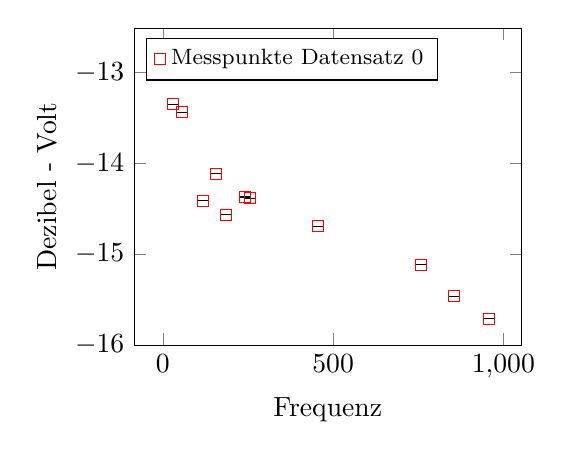
\begin{tikzpicture}
		\pgfplotsset{width=6.5cm,compat=1.3,legend style={font=\footnotesize}}
		\begin{axis}[xlabel={Frequenz},ylabel={Dezibel - Volt},legend cell align=left,legend pos=north west]
		
\addplot+[only marks,color=red,mark=square,error bars/.cd,x dir=both,x explicit,y dir=both,y explicit,error bar style={color=black}] table[x=X,y=Y,x error=xerror,y error=yerror,row sep=\\]{
			X	Y	xerror	yerror	\\
			 10.253906 	 -12.80232 	 0 	 0 	\\
			 30.761719 	 -13.347933 	 0 	 0 	\\
			 57.128906 	 -13.436821 	 0 	 0 	\\
			 118.652344 	 -14.413613 	 0 	 0 	\\
			 156.738281 	 -14.114061 	 0 	 0 	\\
			 184.570312 	 -14.565412 	 0 	 0 	\\
			 241.699219 	 -14.37053 	 0 	 0 	\\
			 254.882812 	 -14.385941 	 0 	 0 	\\
			 455.566406 	 -14.692671 	 0 	 0 	\\
			 757.324219 	 -15.117664 	 0 	 0 	\\
			 855.46875 	 -15.462831 	 0 	 0 	\\
			 958.007812 	 -15.711401 	 0 	 0 	\\
		};
		\addlegendentry{Messpunkte Datensatz 0}

		\end{axis}
		\end{tikzpicture}
	\caption{Umgebung}
	\label{fig:Umgebungsmessung}
\end{figure}

        %% \begin{figure}[H]

	\centering
	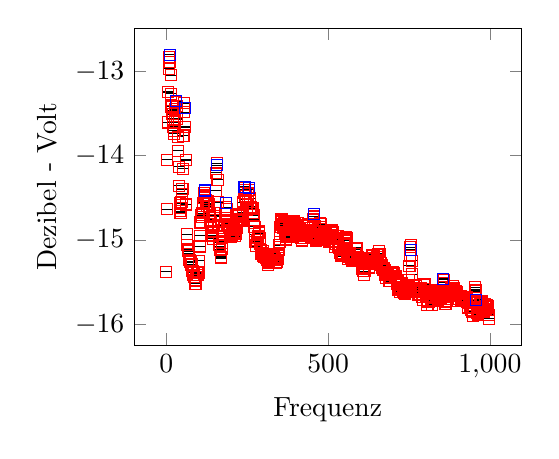
\begin{tikzpicture}
		\pgfplotsset{width=6.5cm,compat=1.3,legend style={font=\footnotesize}}
		\begin{axis}[xlabel={Frequenz},ylabel={Dezibel - Volt},legend cell align=left,legend pos=north west]
		
\addplot+[only marks,color=red,mark=square,error bars/.cd,x dir=both,x explicit,y dir=both,y explicit,error bar style={color=black}] table[x=X,y=Y,x error=xerror,y error=yerror,row sep=\\]{
			X	Y	xerror	yerror	\\
			 0.0 	 -15.377863 	 0 	 0 	\\
			 1.464844 	 -14.634824 	 0 	 0 	\\
			 2.929687 	 -14.048924 	 0 	 0 	\\
			 4.394531 	 -13.606714 	 0 	 0 	\\
			 5.859375 	 -13.245078 	 0 	 0 	\\
			 7.324219 	 -12.971722 	 0 	 0 	\\
			 8.789062 	 -12.828342 	 0 	 0 	\\
			 10.253906 	 -12.80232 	 0 	 0 	\\
			 11.71875 	 -12.891995 	 0 	 0 	\\
			 13.183594 	 -13.047378 	 0 	 0 	\\
			 14.648437 	 -13.266726 	 0 	 0 	\\
			 16.113281 	 -13.417296 	 0 	 0 	\\
			 17.578125 	 -13.467953 	 0 	 0 	\\
			 19.042969 	 -13.510851 	 0 	 0 	\\
			 20.507812 	 -13.562329 	 0 	 0 	\\
			 21.972656 	 -13.65778 	 0 	 0 	\\
			 23.4375 	 -13.742413 	 0 	 0 	\\
			 24.902344 	 -13.70612 	 0 	 0 	\\
			 26.367187 	 -13.603597 	 0 	 0 	\\
			 27.832031 	 -13.452496 	 0 	 0 	\\
			 29.296875 	 -13.360224 	 0 	 0 	\\
			 30.761719 	 -13.347933 	 0 	 0 	\\
			 32.226562 	 -13.416004 	 0 	 0 	\\
			 33.691406 	 -13.565305 	 0 	 0 	\\
			 35.15625 	 -13.777465 	 0 	 0 	\\
			 36.621094 	 -13.942297 	 0 	 0 	\\
			 38.085937 	 -14.13413 	 0 	 0 	\\
			 39.550781 	 -14.355808 	 0 	 0 	\\
			 41.015625 	 -14.567138 	 0 	 0 	\\
			 42.480469 	 -14.661787 	 0 	 0 	\\
			 43.945312 	 -14.676044 	 0 	 0 	\\
			 45.410156 	 -14.624667 	 0 	 0 	\\
			 46.875 	 -14.554264 	 0 	 0 	\\
			 48.339844 	 -14.454346 	 0 	 0 	\\
			 49.804687 	 -14.396066 	 0 	 0 	\\
			 51.269531 	 -14.157371 	 0 	 0 	\\
			 52.734375 	 -13.76188 	 0 	 0 	\\
			 54.199219 	 -13.486916 	 0 	 0 	\\
			 55.664062 	 -13.378995 	 0 	 0 	\\
			 57.128906 	 -13.436821 	 0 	 0 	\\
			 58.59375 	 -13.660917 	 0 	 0 	\\
			 60.058594 	 -14.051488 	 0 	 0 	\\
			 61.523437 	 -14.579972 	 0 	 0 	\\
			 62.988281 	 -14.932836 	 0 	 0 	\\
			 64.453125 	 -15.057708 	 0 	 0 	\\
			 65.917969 	 -15.10667 	 0 	 0 	\\
			 67.382812 	 -15.131666 	 0 	 0 	\\
			 68.847656 	 -15.120015 	 0 	 0 	\\
			 70.3125 	 -15.166563 	 0 	 0 	\\
			 71.777344 	 -15.234852 	 0 	 0 	\\
			 73.242187 	 -15.257725 	 0 	 0 	\\
			 74.707031 	 -15.258081 	 0 	 0 	\\
			 76.171875 	 -15.262162 	 0 	 0 	\\
			 77.636719 	 -15.292419 	 0 	 0 	\\
			 79.101562 	 -15.302074 	 0 	 0 	\\
			 80.566406 	 -15.371643 	 0 	 0 	\\
			 82.03125 	 -15.414623 	 0 	 0 	\\
			 83.496094 	 -15.384488 	 0 	 0 	\\
			 84.960937 	 -15.38654 	 0 	 0 	\\
			 86.425781 	 -15.435651 	 0 	 0 	\\
			 87.890625 	 -15.480934 	 0 	 0 	\\
			 89.355469 	 -15.519261 	 0 	 0 	\\
			 90.820312 	 -15.520492 	 0 	 0 	\\
			 92.285156 	 -15.435193 	 0 	 0 	\\
			 93.75 	 -15.419489 	 0 	 0 	\\
			 95.214844 	 -15.394684 	 0 	 0 	\\
			 96.679687 	 -15.392082 	 0 	 0 	\\
			 98.144531 	 -15.417509 	 0 	 0 	\\
			 99.609375 	 -15.390234 	 0 	 0 	\\
			 101.074219 	 -15.246798 	 0 	 0 	\\
			 102.539062 	 -15.077027 	 0 	 0 	\\
			 104.003906 	 -14.951796 	 0 	 0 	\\
			 105.46875 	 -14.793155 	 0 	 0 	\\
			 106.933594 	 -14.725076 	 0 	 0 	\\
			 108.398437 	 -14.70885 	 0 	 0 	\\
			 109.863281 	 -14.729992 	 0 	 0 	\\
			 111.328125 	 -14.683022 	 0 	 0 	\\
			 112.792969 	 -14.633574 	 0 	 0 	\\
			 114.257812 	 -14.559146 	 0 	 0 	\\
			 115.722656 	 -14.497235 	 0 	 0 	\\
			 117.1875 	 -14.442762 	 0 	 0 	\\
			 118.652344 	 -14.413613 	 0 	 0 	\\
			 120.117187 	 -14.473501 	 0 	 0 	\\
			 121.582031 	 -14.529763 	 0 	 0 	\\
			 123.046875 	 -14.572319 	 0 	 0 	\\
			 124.511719 	 -14.599137 	 0 	 0 	\\
			 125.976562 	 -14.57376 	 0 	 0 	\\
			 127.441406 	 -14.5452 	 0 	 0 	\\
			 128.90625 	 -14.577725 	 0 	 0 	\\
			 130.371094 	 -14.570568 	 0 	 0 	\\
			 131.835937 	 -14.606959 	 0 	 0 	\\
			 133.300781 	 -14.677834 	 0 	 0 	\\
			 134.765625 	 -14.72607 	 0 	 0 	\\
			 136.230469 	 -14.783752 	 0 	 0 	\\
			 137.695312 	 -14.845978 	 0 	 0 	\\
			 139.160156 	 -14.890022 	 0 	 0 	\\
			 140.625 	 -14.942508 	 0 	 0 	\\
			 142.089844 	 -14.958278 	 0 	 0 	\\
			 143.554687 	 -14.984087 	 0 	 0 	\\
			 145.019531 	 -14.907987 	 0 	 0 	\\
			 146.484375 	 -14.833804 	 0 	 0 	\\
			 147.949219 	 -14.760233 	 0 	 0 	\\
			 149.414062 	 -14.716789 	 0 	 0 	\\
			 150.878906 	 -14.612332 	 0 	 0 	\\
			 152.34375 	 -14.415131 	 0 	 0 	\\
			 153.808594 	 -14.203882 	 0 	 0 	\\
			 155.273437 	 -14.090973 	 0 	 0 	\\
			 156.738281 	 -14.114061 	 0 	 0 	\\
			 158.203125 	 -14.28813 	 0 	 0 	\\
			 159.667969 	 -14.549723 	 0 	 0 	\\
			 161.132812 	 -14.826476 	 0 	 0 	\\
			 162.597656 	 -15.024029 	 0 	 0 	\\
			 164.0625 	 -15.059548 	 0 	 0 	\\
			 165.527344 	 -15.076732 	 0 	 0 	\\
			 166.992187 	 -15.118956 	 0 	 0 	\\
			 168.457031 	 -15.214337 	 0 	 0 	\\
			 169.921875 	 -15.197879 	 0 	 0 	\\
			 171.386719 	 -15.102572 	 0 	 0 	\\
			 172.851562 	 -15.033952 	 0 	 0 	\\
			 174.316406 	 -14.968841 	 0 	 0 	\\
			 175.78125 	 -14.886593 	 0 	 0 	\\
			 177.246094 	 -14.857826 	 0 	 0 	\\
			 178.710937 	 -14.834681 	 0 	 0 	\\
			 180.175781 	 -14.781653 	 0 	 0 	\\
			 181.640625 	 -14.697632 	 0 	 0 	\\
			 183.105469 	 -14.612491 	 0 	 0 	\\
			 184.570312 	 -14.565412 	 0 	 0 	\\
			 186.035156 	 -14.630101 	 0 	 0 	\\
			 187.5 	 -14.763068 	 0 	 0 	\\
			 188.964844 	 -14.81181 	 0 	 0 	\\
			 190.429687 	 -14.809167 	 0 	 0 	\\
			 191.894531 	 -14.820498 	 0 	 0 	\\
			 193.359375 	 -14.83837 	 0 	 0 	\\
			 194.824219 	 -14.842676 	 0 	 0 	\\
			 196.289062 	 -14.914527 	 0 	 0 	\\
			 197.753906 	 -14.937226 	 0 	 0 	\\
			 199.21875 	 -14.963659 	 0 	 0 	\\
			 200.683594 	 -14.964335 	 0 	 0 	\\
			 202.148437 	 -14.949748 	 0 	 0 	\\
			 203.613281 	 -14.918795 	 0 	 0 	\\
			 205.078125 	 -14.910389 	 0 	 0 	\\
			 206.542969 	 -14.885805 	 0 	 0 	\\
			 208.007812 	 -14.866659 	 0 	 0 	\\
			 209.472656 	 -14.877181 	 0 	 0 	\\
			 210.9375 	 -14.919722 	 0 	 0 	\\
			 212.402344 	 -14.957385 	 0 	 0 	\\
			 213.867187 	 -14.929474 	 0 	 0 	\\
			 215.332031 	 -14.902048 	 0 	 0 	\\
			 216.796875 	 -14.855239 	 0 	 0 	\\
			 218.261719 	 -14.814927 	 0 	 0 	\\
			 219.726562 	 -14.754177 	 0 	 0 	\\
			 221.191406 	 -14.698331 	 0 	 0 	\\
			 222.65625 	 -14.7121 	 0 	 0 	\\
			 224.121094 	 -14.720584 	 0 	 0 	\\
			 225.585937 	 -14.752912 	 0 	 0 	\\
			 227.050781 	 -14.754292 	 0 	 0 	\\
			 228.515625 	 -14.7607 	 0 	 0 	\\
			 229.980469 	 -14.754367 	 0 	 0 	\\
			 231.445312 	 -14.766731 	 0 	 0 	\\
			 232.910156 	 -14.774063 	 0 	 0 	\\
			 234.375 	 -14.75994 	 0 	 0 	\\
			 235.839844 	 -14.672699 	 0 	 0 	\\
			 237.304687 	 -14.553177 	 0 	 0 	\\
			 238.769531 	 -14.442574 	 0 	 0 	\\
			 240.234375 	 -14.380149 	 0 	 0 	\\
			 241.699219 	 -14.37053 	 0 	 0 	\\
			 243.164062 	 -14.405877 	 0 	 0 	\\
			 244.628906 	 -14.478126 	 0 	 0 	\\
			 246.09375 	 -14.525214 	 0 	 0 	\\
			 247.558594 	 -14.571617 	 0 	 0 	\\
			 249.023437 	 -14.640223 	 0 	 0 	\\
			 250.488281 	 -14.62722 	 0 	 0 	\\
			 251.953125 	 -14.545152 	 0 	 0 	\\
			 253.417969 	 -14.450371 	 0 	 0 	\\
			 254.882812 	 -14.385941 	 0 	 0 	\\
			 256.347656 	 -14.403229 	 0 	 0 	\\
			 257.8125 	 -14.507634 	 0 	 0 	\\
			 259.277344 	 -14.623046 	 0 	 0 	\\
			 260.742187 	 -14.619449 	 0 	 0 	\\
			 262.207031 	 -14.607496 	 0 	 0 	\\
			 263.671875 	 -14.6373 	 0 	 0 	\\
			 265.136719 	 -14.621309 	 0 	 0 	\\
			 266.601562 	 -14.623232 	 0 	 0 	\\
			 268.066406 	 -14.675993 	 0 	 0 	\\
			 269.53125 	 -14.705281 	 0 	 0 	\\
			 270.996094 	 -14.7643 	 0 	 0 	\\
			 272.460937 	 -14.844184 	 0 	 0 	\\
			 273.925781 	 -14.933865 	 0 	 0 	\\
			 275.390625 	 -15.023675 	 0 	 0 	\\
			 276.855469 	 -15.074193 	 0 	 0 	\\
			 278.320312 	 -15.070534 	 0 	 0 	\\
			 279.785156 	 -15.020149 	 0 	 0 	\\
			 281.25 	 -14.997145 	 0 	 0 	\\
			 282.714844 	 -14.974335 	 0 	 0 	\\
			 284.179687 	 -14.95966 	 0 	 0 	\\
			 285.644531 	 -14.900165 	 0 	 0 	\\
			 287.109375 	 -14.919175 	 0 	 0 	\\
			 288.574219 	 -14.978309 	 0 	 0 	\\
			 290.039062 	 -15.051671 	 0 	 0 	\\
			 291.503906 	 -15.121433 	 0 	 0 	\\
			 292.96875 	 -15.166601 	 0 	 0 	\\
			 294.433594 	 -15.162406 	 0 	 0 	\\
			 295.898437 	 -15.158841 	 0 	 0 	\\
			 297.363281 	 -15.136656 	 0 	 0 	\\
			 298.828125 	 -15.155136 	 0 	 0 	\\
			 300.292969 	 -15.186434 	 0 	 0 	\\
			 301.757812 	 -15.204195 	 0 	 0 	\\
			 303.222656 	 -15.177276 	 0 	 0 	\\
			 304.6875 	 -15.183911 	 0 	 0 	\\
			 306.152344 	 -15.169498 	 0 	 0 	\\
			 307.617187 	 -15.183561 	 0 	 0 	\\
			 309.082031 	 -15.208333 	 0 	 0 	\\
			 310.546875 	 -15.236216 	 0 	 0 	\\
			 312.011719 	 -15.223957 	 0 	 0 	\\
			 313.476562 	 -15.265625 	 0 	 0 	\\
			 314.941406 	 -15.293078 	 0 	 0 	\\
			 316.40625 	 -15.269928 	 0 	 0 	\\
			 317.871094 	 -15.246589 	 0 	 0 	\\
			 319.335937 	 -15.235773 	 0 	 0 	\\
			 320.800781 	 -15.236421 	 0 	 0 	\\
			 322.265625 	 -15.202186 	 0 	 0 	\\
			 323.730469 	 -15.174848 	 0 	 0 	\\
			 325.195312 	 -15.166102 	 0 	 0 	\\
			 326.660156 	 -15.188197 	 0 	 0 	\\
			 328.125 	 -15.181395 	 0 	 0 	\\
			 329.589844 	 -15.162683 	 0 	 0 	\\
			 331.054687 	 -15.166449 	 0 	 0 	\\
			 332.519531 	 -15.196976 	 0 	 0 	\\
			 333.984375 	 -15.217628 	 0 	 0 	\\
			 335.449219 	 -15.211973 	 0 	 0 	\\
			 336.914062 	 -15.242704 	 0 	 0 	\\
			 338.378906 	 -15.267842 	 0 	 0 	\\
			 339.84375 	 -15.270764 	 0 	 0 	\\
			 341.308594 	 -15.259543 	 0 	 0 	\\
			 342.773437 	 -15.233829 	 0 	 0 	\\
			 344.238281 	 -15.219391 	 0 	 0 	\\
			 345.703125 	 -15.173472 	 0 	 0 	\\
			 347.167969 	 -15.116821 	 0 	 0 	\\
			 348.632812 	 -15.060204 	 0 	 0 	\\
			 350.097656 	 -15.020687 	 0 	 0 	\\
			 351.5625 	 -14.95811 	 0 	 0 	\\
			 353.027344 	 -14.843255 	 0 	 0 	\\
			 354.492187 	 -14.770459 	 0 	 0 	\\
			 355.957031 	 -14.749877 	 0 	 0 	\\
			 357.421875 	 -14.790935 	 0 	 0 	\\
			 358.886719 	 -14.815091 	 0 	 0 	\\
			 360.351562 	 -14.829277 	 0 	 0 	\\
			 361.816406 	 -14.859088 	 0 	 0 	\\
			 363.28125 	 -14.840884 	 0 	 0 	\\
			 364.746094 	 -14.800479 	 0 	 0 	\\
			 366.210937 	 -14.83119 	 0 	 0 	\\
			 367.675781 	 -14.922398 	 0 	 0 	\\
			 369.140625 	 -14.984439 	 0 	 0 	\\
			 370.605469 	 -15.002639 	 0 	 0 	\\
			 372.070312 	 -14.9656 	 0 	 0 	\\
			 373.535156 	 -14.9294 	 0 	 0 	\\
			 375.0 	 -14.915619 	 0 	 0 	\\
			 376.464844 	 -14.935517 	 0 	 0 	\\
			 377.929687 	 -14.91687 	 0 	 0 	\\
			 379.394531 	 -14.875338 	 0 	 0 	\\
			 380.859375 	 -14.886914 	 0 	 0 	\\
			 382.324219 	 -14.926704 	 0 	 0 	\\
			 383.789062 	 -14.958619 	 0 	 0 	\\
			 385.253906 	 -14.929833 	 0 	 0 	\\
			 386.71875 	 -14.858562 	 0 	 0 	\\
			 388.183594 	 -14.86051 	 0 	 0 	\\
			 389.648437 	 -14.830076 	 0 	 0 	\\
			 391.113281 	 -14.821938 	 0 	 0 	\\
			 392.578125 	 -14.818603 	 0 	 0 	\\
			 394.042969 	 -14.787719 	 0 	 0 	\\
			 395.507812 	 -14.77604 	 0 	 0 	\\
			 396.972656 	 -14.806179 	 0 	 0 	\\
			 398.4375 	 -14.859224 	 0 	 0 	\\
			 399.902344 	 -14.943791 	 0 	 0 	\\
			 401.367187 	 -14.912992 	 0 	 0 	\\
			 402.832031 	 -14.871232 	 0 	 0 	\\
			 404.296875 	 -14.852966 	 0 	 0 	\\
			 405.761719 	 -14.800711 	 0 	 0 	\\
			 407.226562 	 -14.830097 	 0 	 0 	\\
			 408.691406 	 -14.862748 	 0 	 0 	\\
			 410.15625 	 -14.903424 	 0 	 0 	\\
			 411.621094 	 -14.881023 	 0 	 0 	\\
			 413.085937 	 -14.860914 	 0 	 0 	\\
			 414.550781 	 -14.886766 	 0 	 0 	\\
			 416.015625 	 -14.925458 	 0 	 0 	\\
			 417.480469 	 -14.982026 	 0 	 0 	\\
			 418.945312 	 -14.996119 	 0 	 0 	\\
			 420.410156 	 -15.012344 	 0 	 0 	\\
			 421.875 	 -14.978925 	 0 	 0 	\\
			 423.339844 	 -14.979966 	 0 	 0 	\\
			 424.804687 	 -14.976032 	 0 	 0 	\\
			 426.269531 	 -14.953691 	 0 	 0 	\\
			 427.734375 	 -14.937518 	 0 	 0 	\\
			 429.199219 	 -14.914414 	 0 	 0 	\\
			 430.664062 	 -14.898355 	 0 	 0 	\\
			 432.128906 	 -14.90933 	 0 	 0 	\\
			 433.59375 	 -14.904637 	 0 	 0 	\\
			 435.058594 	 -14.859341 	 0 	 0 	\\
			 436.523437 	 -14.821858 	 0 	 0 	\\
			 437.988281 	 -14.816956 	 0 	 0 	\\
			 439.453125 	 -14.840019 	 0 	 0 	\\
			 440.917969 	 -14.905879 	 0 	 0 	\\
			 442.382812 	 -14.931551 	 0 	 0 	\\
			 443.847656 	 -14.948507 	 0 	 0 	\\
			 445.3125 	 -14.957315 	 0 	 0 	\\
			 446.777344 	 -14.962708 	 0 	 0 	\\
			 448.242187 	 -14.959279 	 0 	 0 	\\
			 449.707031 	 -14.976118 	 0 	 0 	\\
			 451.171875 	 -14.958943 	 0 	 0 	\\
			 452.636719 	 -14.887534 	 0 	 0 	\\
			 454.101562 	 -14.757729 	 0 	 0 	\\
			 455.566406 	 -14.692671 	 0 	 0 	\\
			 457.03125 	 -14.722008 	 0 	 0 	\\
			 458.496094 	 -14.836651 	 0 	 0 	\\
			 459.960937 	 -14.94227 	 0 	 0 	\\
			 461.425781 	 -15.008921 	 0 	 0 	\\
			 462.890625 	 -14.996549 	 0 	 0 	\\
			 464.355469 	 -14.985025 	 0 	 0 	\\
			 465.820312 	 -14.988841 	 0 	 0 	\\
			 467.285156 	 -14.959832 	 0 	 0 	\\
			 468.75 	 -14.963813 	 0 	 0 	\\
			 470.214844 	 -14.904158 	 0 	 0 	\\
			 471.679687 	 -14.899158 	 0 	 0 	\\
			 473.144531 	 -14.90094 	 0 	 0 	\\
			 474.609375 	 -14.848906 	 0 	 0 	\\
			 476.074219 	 -14.804283 	 0 	 0 	\\
			 477.539062 	 -14.812484 	 0 	 0 	\\
			 479.003906 	 -14.873761 	 0 	 0 	\\
			 480.46875 	 -14.889497 	 0 	 0 	\\
			 481.933594 	 -14.94114 	 0 	 0 	\\
			 483.398437 	 -14.959876 	 0 	 0 	\\
			 484.863281 	 -14.981784 	 0 	 0 	\\
			 486.328125 	 -15.002628 	 0 	 0 	\\
			 487.792969 	 -14.986382 	 0 	 0 	\\
			 489.257812 	 -14.958831 	 0 	 0 	\\
			 490.722656 	 -14.924504 	 0 	 0 	\\
			 492.1875 	 -14.919779 	 0 	 0 	\\
			 493.652344 	 -14.916625 	 0 	 0 	\\
			 495.117187 	 -14.949242 	 0 	 0 	\\
			 496.582031 	 -14.962884 	 0 	 0 	\\
			 498.046875 	 -14.955165 	 0 	 0 	\\
			 499.511719 	 -14.956127 	 0 	 0 	\\
			 500.976562 	 -14.98079 	 0 	 0 	\\
			 502.441406 	 -15.013497 	 0 	 0 	\\
			 503.90625 	 -15.017682 	 0 	 0 	\\
			 505.371094 	 -14.968866 	 0 	 0 	\\
			 506.835937 	 -14.974244 	 0 	 0 	\\
			 508.300781 	 -14.9413 	 0 	 0 	\\
			 509.765625 	 -14.899098 	 0 	 0 	\\
			 511.230469 	 -14.881912 	 0 	 0 	\\
			 512.695312 	 -14.900233 	 0 	 0 	\\
			 514.160156 	 -14.912839 	 0 	 0 	\\
			 515.625 	 -14.946873 	 0 	 0 	\\
			 517.089844 	 -14.979354 	 0 	 0 	\\
			 518.554687 	 -15.00894 	 0 	 0 	\\
			 520.019531 	 -15.051378 	 0 	 0 	\\
			 521.484375 	 -15.07899 	 0 	 0 	\\
			 522.949219 	 -15.042952 	 0 	 0 	\\
			 524.414062 	 -15.007503 	 0 	 0 	\\
			 525.878906 	 -14.988524 	 0 	 0 	\\
			 527.34375 	 -14.957197 	 0 	 0 	\\
			 528.808594 	 -14.957643 	 0 	 0 	\\
			 530.273437 	 -14.989294 	 0 	 0 	\\
			 531.738281 	 -15.07429 	 0 	 0 	\\
			 533.203125 	 -15.091988 	 0 	 0 	\\
			 534.667969 	 -15.084726 	 0 	 0 	\\
			 536.132812 	 -15.118594 	 0 	 0 	\\
			 537.597656 	 -15.153552 	 0 	 0 	\\
			 539.0625 	 -15.189469 	 0 	 0 	\\
			 540.527344 	 -15.190528 	 0 	 0 	\\
			 541.992187 	 -15.173378 	 0 	 0 	\\
			 543.457031 	 -15.178132 	 0 	 0 	\\
			 544.921875 	 -15.165173 	 0 	 0 	\\
			 546.386719 	 -15.114103 	 0 	 0 	\\
			 547.851562 	 -15.103409 	 0 	 0 	\\
			 549.316406 	 -15.065115 	 0 	 0 	\\
			 550.78125 	 -15.039258 	 0 	 0 	\\
			 552.246094 	 -15.00732 	 0 	 0 	\\
			 553.710937 	 -14.994949 	 0 	 0 	\\
			 555.175781 	 -14.970948 	 0 	 0 	\\
			 556.640625 	 -14.973621 	 0 	 0 	\\
			 558.105469 	 -15.052147 	 0 	 0 	\\
			 559.570312 	 -15.154666 	 0 	 0 	\\
			 561.035156 	 -15.223556 	 0 	 0 	\\
			 562.5 	 -15.205299 	 0 	 0 	\\
			 563.964844 	 -15.185758 	 0 	 0 	\\
			 565.429687 	 -15.153672 	 0 	 0 	\\
			 566.894531 	 -15.161342 	 0 	 0 	\\
			 568.359375 	 -15.174439 	 0 	 0 	\\
			 569.824219 	 -15.223043 	 0 	 0 	\\
			 571.289062 	 -15.226492 	 0 	 0 	\\
			 572.753906 	 -15.244243 	 0 	 0 	\\
			 574.21875 	 -15.246913 	 0 	 0 	\\
			 575.683594 	 -15.249243 	 0 	 0 	\\
			 577.148437 	 -15.218895 	 0 	 0 	\\
			 578.613281 	 -15.21606 	 0 	 0 	\\
			 580.078125 	 -15.209814 	 0 	 0 	\\
			 581.542969 	 -15.22923 	 0 	 0 	\\
			 583.007812 	 -15.202847 	 0 	 0 	\\
			 584.472656 	 -15.168714 	 0 	 0 	\\
			 585.9375 	 -15.112795 	 0 	 0 	\\
			 587.402344 	 -15.093079 	 0 	 0 	\\
			 588.867187 	 -15.099123 	 0 	 0 	\\
			 590.332031 	 -15.169947 	 0 	 0 	\\
			 591.796875 	 -15.199622 	 0 	 0 	\\
			 593.261719 	 -15.229956 	 0 	 0 	\\
			 594.726562 	 -15.235358 	 0 	 0 	\\
			 596.191406 	 -15.214944 	 0 	 0 	\\
			 597.65625 	 -15.24572 	 0 	 0 	\\
			 599.121094 	 -15.22883 	 0 	 0 	\\
			 600.585937 	 -15.231044 	 0 	 0 	\\
			 602.050781 	 -15.238379 	 0 	 0 	\\
			 603.515625 	 -15.2394 	 0 	 0 	\\
			 604.980469 	 -15.283166 	 0 	 0 	\\
			 606.445312 	 -15.340901 	 0 	 0 	\\
			 607.910156 	 -15.335839 	 0 	 0 	\\
			 609.375 	 -15.37254 	 0 	 0 	\\
			 610.839844 	 -15.413192 	 0 	 0 	\\
			 612.304687 	 -15.373417 	 0 	 0 	\\
			 613.769531 	 -15.323639 	 0 	 0 	\\
			 615.234375 	 -15.275425 	 0 	 0 	\\
			 616.699219 	 -15.263429 	 0 	 0 	\\
			 618.164062 	 -15.250132 	 0 	 0 	\\
			 619.628906 	 -15.267253 	 0 	 0 	\\
			 621.09375 	 -15.26846 	 0 	 0 	\\
			 622.558594 	 -15.248096 	 0 	 0 	\\
			 624.023437 	 -15.281112 	 0 	 0 	\\
			 625.488281 	 -15.332221 	 0 	 0 	\\
			 626.953125 	 -15.325418 	 0 	 0 	\\
			 628.417969 	 -15.289986 	 0 	 0 	\\
			 629.882812 	 -15.286293 	 0 	 0 	\\
			 631.347656 	 -15.279109 	 0 	 0 	\\
			 632.8125 	 -15.259318 	 0 	 0 	\\
			 634.277344 	 -15.219471 	 0 	 0 	\\
			 635.742187 	 -15.190152 	 0 	 0 	\\
			 637.207031 	 -15.17394 	 0 	 0 	\\
			 638.671875 	 -15.185223 	 0 	 0 	\\
			 640.136719 	 -15.193695 	 0 	 0 	\\
			 641.601562 	 -15.229764 	 0 	 0 	\\
			 643.066406 	 -15.250337 	 0 	 0 	\\
			 644.53125 	 -15.272403 	 0 	 0 	\\
			 645.996094 	 -15.274543 	 0 	 0 	\\
			 647.460937 	 -15.258597 	 0 	 0 	\\
			 648.925781 	 -15.25687 	 0 	 0 	\\
			 650.390625 	 -15.235247 	 0 	 0 	\\
			 651.855469 	 -15.174024 	 0 	 0 	\\
			 653.320312 	 -15.177223 	 0 	 0 	\\
			 654.785156 	 -15.166174 	 0 	 0 	\\
			 656.25 	 -15.136456 	 0 	 0 	\\
			 657.714844 	 -15.134069 	 0 	 0 	\\
			 659.179687 	 -15.172512 	 0 	 0 	\\
			 660.644531 	 -15.200877 	 0 	 0 	\\
			 662.109375 	 -15.271783 	 0 	 0 	\\
			 663.574219 	 -15.292622 	 0 	 0 	\\
			 665.039062 	 -15.30175 	 0 	 0 	\\
			 666.503906 	 -15.322372 	 0 	 0 	\\
			 667.96875 	 -15.334441 	 0 	 0 	\\
			 669.433594 	 -15.342618 	 0 	 0 	\\
			 670.898437 	 -15.354524 	 0 	 0 	\\
			 672.363281 	 -15.332675 	 0 	 0 	\\
			 673.828125 	 -15.351229 	 0 	 0 	\\
			 675.292969 	 -15.355035 	 0 	 0 	\\
			 676.757812 	 -15.410555 	 0 	 0 	\\
			 678.222656 	 -15.454251 	 0 	 0 	\\
			 679.6875 	 -15.40483 	 0 	 0 	\\
			 681.152344 	 -15.387011 	 0 	 0 	\\
			 682.617187 	 -15.381831 	 0 	 0 	\\
			 684.082031 	 -15.380513 	 0 	 0 	\\
			 685.546875 	 -15.413772 	 0 	 0 	\\
			 687.011719 	 -15.445245 	 0 	 0 	\\
			 688.476562 	 -15.487407 	 0 	 0 	\\
			 689.941406 	 -15.484309 	 0 	 0 	\\
			 691.40625 	 -15.482493 	 0 	 0 	\\
			 692.871094 	 -15.439923 	 0 	 0 	\\
			 694.335937 	 -15.407051 	 0 	 0 	\\
			 695.800781 	 -15.395723 	 0 	 0 	\\
			 697.265625 	 -15.401745 	 0 	 0 	\\
			 698.730469 	 -15.391471 	 0 	 0 	\\
			 700.195312 	 -15.385299 	 0 	 0 	\\
			 701.660156 	 -15.398126 	 0 	 0 	\\
			 703.125 	 -15.406516 	 0 	 0 	\\
			 704.589844 	 -15.389331 	 0 	 0 	\\
			 706.054687 	 -15.427444 	 0 	 0 	\\
			 707.519531 	 -15.431758 	 0 	 0 	\\
			 708.984375 	 -15.425674 	 0 	 0 	\\
			 710.449219 	 -15.446452 	 0 	 0 	\\
			 711.914062 	 -15.474679 	 0 	 0 	\\
			 713.378906 	 -15.525805 	 0 	 0 	\\
			 714.84375 	 -15.589171 	 0 	 0 	\\
			 716.308594 	 -15.586641 	 0 	 0 	\\
			 717.773437 	 -15.587684 	 0 	 0 	\\
			 719.238281 	 -15.595326 	 0 	 0 	\\
			 720.703125 	 -15.593172 	 0 	 0 	\\
			 722.167969 	 -15.615338 	 0 	 0 	\\
			 723.632812 	 -15.574624 	 0 	 0 	\\
			 725.097656 	 -15.560847 	 0 	 0 	\\
			 726.5625 	 -15.50968 	 0 	 0 	\\
			 728.027344 	 -15.50755 	 0 	 0 	\\
			 729.492187 	 -15.529643 	 0 	 0 	\\
			 730.957031 	 -15.584285 	 0 	 0 	\\
			 732.421875 	 -15.61486 	 0 	 0 	\\
			 733.886719 	 -15.607152 	 0 	 0 	\\
			 735.351562 	 -15.62397 	 0 	 0 	\\
			 736.816406 	 -15.634898 	 0 	 0 	\\
			 738.28125 	 -15.635034 	 0 	 0 	\\
			 739.746094 	 -15.61694 	 0 	 0 	\\
			 741.210937 	 -15.600624 	 0 	 0 	\\
			 742.675781 	 -15.597813 	 0 	 0 	\\
			 744.140625 	 -15.580082 	 0 	 0 	\\
			 745.605469 	 -15.576345 	 0 	 0 	\\
			 747.070312 	 -15.593973 	 0 	 0 	\\
			 748.535156 	 -15.552722 	 0 	 0 	\\
			 750.0 	 -15.48038 	 0 	 0 	\\
			 751.464844 	 -15.305891 	 0 	 0 	\\
			 752.929687 	 -15.187352 	 0 	 0 	\\
			 754.394531 	 -15.086647 	 0 	 0 	\\
			 755.859375 	 -15.058162 	 0 	 0 	\\
			 757.324219 	 -15.117664 	 0 	 0 	\\
			 758.789062 	 -15.246047 	 0 	 0 	\\
			 760.253906 	 -15.409334 	 0 	 0 	\\
			 761.71875 	 -15.531305 	 0 	 0 	\\
			 763.183594 	 -15.610576 	 0 	 0 	\\
			 764.648437 	 -15.608558 	 0 	 0 	\\
			 766.113281 	 -15.611633 	 0 	 0 	\\
			 767.578125 	 -15.588454 	 0 	 0 	\\
			 769.042969 	 -15.592371 	 0 	 0 	\\
			 770.507812 	 -15.545033 	 0 	 0 	\\
			 771.972656 	 -15.570368 	 0 	 0 	\\
			 773.4375 	 -15.590781 	 0 	 0 	\\
			 774.902344 	 -15.607064 	 0 	 0 	\\
			 776.367187 	 -15.585898 	 0 	 0 	\\
			 777.832031 	 -15.577243 	 0 	 0 	\\
			 779.296875 	 -15.646981 	 0 	 0 	\\
			 780.761719 	 -15.643249 	 0 	 0 	\\
			 782.226562 	 -15.638178 	 0 	 0 	\\
			 783.691406 	 -15.638564 	 0 	 0 	\\
			 785.15625 	 -15.600507 	 0 	 0 	\\
			 786.621094 	 -15.619703 	 0 	 0 	\\
			 788.085937 	 -15.571874 	 0 	 0 	\\
			 789.550781 	 -15.611286 	 0 	 0 	\\
			 791.015625 	 -15.679298 	 0 	 0 	\\
			 792.480469 	 -15.708989 	 0 	 0 	\\
			 793.945312 	 -15.715225 	 0 	 0 	\\
			 795.410156 	 -15.608697 	 0 	 0 	\\
			 796.875 	 -15.524976 	 0 	 0 	\\
			 798.339844 	 -15.528546 	 0 	 0 	\\
			 799.804687 	 -15.58165 	 0 	 0 	\\
			 801.269531 	 -15.617491 	 0 	 0 	\\
			 802.734375 	 -15.636778 	 0 	 0 	\\
			 804.199219 	 -15.671623 	 0 	 0 	\\
			 805.664062 	 -15.730237 	 0 	 0 	\\
			 807.128906 	 -15.773552 	 0 	 0 	\\
			 808.59375 	 -15.735681 	 0 	 0 	\\
			 810.058594 	 -15.737674 	 0 	 0 	\\
			 811.523437 	 -15.668612 	 0 	 0 	\\
			 812.988281 	 -15.63689 	 0 	 0 	\\
			 814.453125 	 -15.62498 	 0 	 0 	\\
			 815.917969 	 -15.617883 	 0 	 0 	\\
			 817.382812 	 -15.666109 	 0 	 0 	\\
			 818.847656 	 -15.717725 	 0 	 0 	\\
			 820.3125 	 -15.769734 	 0 	 0 	\\
			 821.777344 	 -15.72365 	 0 	 0 	\\
			 823.242187 	 -15.688064 	 0 	 0 	\\
			 824.707031 	 -15.715984 	 0 	 0 	\\
			 826.171875 	 -15.6625 	 0 	 0 	\\
			 827.636719 	 -15.61216 	 0 	 0 	\\
			 829.101562 	 -15.623609 	 0 	 0 	\\
			 830.566406 	 -15.595214 	 0 	 0 	\\
			 832.03125 	 -15.627422 	 0 	 0 	\\
			 833.496094 	 -15.660074 	 0 	 0 	\\
			 834.960937 	 -15.659803 	 0 	 0 	\\
			 836.425781 	 -15.679097 	 0 	 0 	\\
			 837.890625 	 -15.684159 	 0 	 0 	\\
			 839.355469 	 -15.704955 	 0 	 0 	\\
			 840.820312 	 -15.718154 	 0 	 0 	\\
			 842.285156 	 -15.682697 	 0 	 0 	\\
			 843.75 	 -15.641373 	 0 	 0 	\\
			 845.214844 	 -15.62105 	 0 	 0 	\\
			 846.679687 	 -15.658638 	 0 	 0 	\\
			 848.144531 	 -15.666164 	 0 	 0 	\\
			 849.609375 	 -15.682085 	 0 	 0 	\\
			 851.074219 	 -15.664447 	 0 	 0 	\\
			 852.539062 	 -15.590643 	 0 	 0 	\\
			 854.003906 	 -15.506291 	 0 	 0 	\\
			 855.46875 	 -15.462831 	 0 	 0 	\\
			 856.933594 	 -15.474423 	 0 	 0 	\\
			 858.398437 	 -15.560124 	 0 	 0 	\\
			 859.863281 	 -15.633947 	 0 	 0 	\\
			 861.328125 	 -15.72679 	 0 	 0 	\\
			 862.792969 	 -15.760758 	 0 	 0 	\\
			 864.257812 	 -15.731995 	 0 	 0 	\\
			 865.722656 	 -15.702384 	 0 	 0 	\\
			 867.1875 	 -15.67397 	 0 	 0 	\\
			 868.652344 	 -15.662891 	 0 	 0 	\\
			 870.117187 	 -15.630239 	 0 	 0 	\\
			 871.582031 	 -15.635438 	 0 	 0 	\\
			 873.046875 	 -15.621477 	 0 	 0 	\\
			 874.511719 	 -15.60827 	 0 	 0 	\\
			 875.976562 	 -15.62759 	 0 	 0 	\\
			 877.441406 	 -15.594709 	 0 	 0 	\\
			 878.90625 	 -15.585837 	 0 	 0 	\\
			 880.371094 	 -15.570807 	 0 	 0 	\\
			 881.835937 	 -15.572389 	 0 	 0 	\\
			 883.300781 	 -15.580299 	 0 	 0 	\\
			 884.765625 	 -15.577057 	 0 	 0 	\\
			 886.230469 	 -15.550639 	 0 	 0 	\\
			 887.695312 	 -15.574831 	 0 	 0 	\\
			 889.160156 	 -15.662833 	 0 	 0 	\\
			 890.625 	 -15.649592 	 0 	 0 	\\
			 892.089844 	 -15.62271 	 0 	 0 	\\
			 893.554687 	 -15.602035 	 0 	 0 	\\
			 895.019531 	 -15.636141 	 0 	 0 	\\
			 896.484375 	 -15.626822 	 0 	 0 	\\
			 897.949219 	 -15.619872 	 0 	 0 	\\
			 899.414062 	 -15.644022 	 0 	 0 	\\
			 900.878906 	 -15.667616 	 0 	 0 	\\
			 902.34375 	 -15.723701 	 0 	 0 	\\
			 903.808594 	 -15.699232 	 0 	 0 	\\
			 905.273437 	 -15.664368 	 0 	 0 	\\
			 906.738281 	 -15.666367 	 0 	 0 	\\
			 908.203125 	 -15.666335 	 0 	 0 	\\
			 909.667969 	 -15.664598 	 0 	 0 	\\
			 911.132812 	 -15.710565 	 0 	 0 	\\
			 912.597656 	 -15.689029 	 0 	 0 	\\
			 914.0625 	 -15.715661 	 0 	 0 	\\
			 915.527344 	 -15.695117 	 0 	 0 	\\
			 916.992187 	 -15.69187 	 0 	 0 	\\
			 918.457031 	 -15.680548 	 0 	 0 	\\
			 919.921875 	 -15.686535 	 0 	 0 	\\
			 921.386719 	 -15.704471 	 0 	 0 	\\
			 922.851562 	 -15.700725 	 0 	 0 	\\
			 924.316406 	 -15.678341 	 0 	 0 	\\
			 925.78125 	 -15.681353 	 0 	 0 	\\
			 927.246094 	 -15.673534 	 0 	 0 	\\
			 928.710937 	 -15.678921 	 0 	 0 	\\
			 930.175781 	 -15.737279 	 0 	 0 	\\
			 931.640625 	 -15.809987 	 0 	 0 	\\
			 933.105469 	 -15.801069 	 0 	 0 	\\
			 934.570312 	 -15.750958 	 0 	 0 	\\
			 936.035156 	 -15.720745 	 0 	 0 	\\
			 937.5 	 -15.773855 	 0 	 0 	\\
			 938.964844 	 -15.798507 	 0 	 0 	\\
			 940.429687 	 -15.83516 	 0 	 0 	\\
			 941.894531 	 -15.810615 	 0 	 0 	\\
			 943.359375 	 -15.803824 	 0 	 0 	\\
			 944.824219 	 -15.849649 	 0 	 0 	\\
			 946.289062 	 -15.854314 	 0 	 0 	\\
			 947.753906 	 -15.900403 	 0 	 0 	\\
			 949.21875 	 -15.839508 	 0 	 0 	\\
			 950.683594 	 -15.793809 	 0 	 0 	\\
			 952.148437 	 -15.721682 	 0 	 0 	\\
			 953.613281 	 -15.607086 	 0 	 0 	\\
			 955.078125 	 -15.562192 	 0 	 0 	\\
			 956.542969 	 -15.593833 	 0 	 0 	\\
			 958.007812 	 -15.711401 	 0 	 0 	\\
			 959.472656 	 -15.791427 	 0 	 0 	\\
			 960.9375 	 -15.861916 	 0 	 0 	\\
			 962.402344 	 -15.888155 	 0 	 0 	\\
			 963.867187 	 -15.879557 	 0 	 0 	\\
			 965.332031 	 -15.85072 	 0 	 0 	\\
			 966.796875 	 -15.826943 	 0 	 0 	\\
			 968.261719 	 -15.809572 	 0 	 0 	\\
			 969.726562 	 -15.762745 	 0 	 0 	\\
			 971.191406 	 -15.739539 	 0 	 0 	\\
			 972.65625 	 -15.739934 	 0 	 0 	\\
			 974.121094 	 -15.730753 	 0 	 0 	\\
			 975.585937 	 -15.749772 	 0 	 0 	\\
			 977.050781 	 -15.812438 	 0 	 0 	\\
			 978.515625 	 -15.826443 	 0 	 0 	\\
			 979.980469 	 -15.817046 	 0 	 0 	\\
			 981.445312 	 -15.848172 	 0 	 0 	\\
			 982.910156 	 -15.855113 	 0 	 0 	\\
			 984.375 	 -15.785814 	 0 	 0 	\\
			 985.839844 	 -15.756446 	 0 	 0 	\\
			 987.304687 	 -15.786946 	 0 	 0 	\\
			 988.769531 	 -15.817096 	 0 	 0 	\\
			 990.234375 	 -15.794719 	 0 	 0 	\\
			 991.699219 	 -15.768299 	 0 	 0 	\\
			 993.164062 	 -15.787708 	 0 	 0 	\\
			 994.628906 	 -15.828947 	 0 	 0 	\\
			 996.09375 	 -15.887351 	 0 	 0 	\\
			 997.558594 	 -15.934677 	 0 	 0 	\\
		};
		% \addlegendentry{Messpunkte Datensatz 0}

\addplot+[only marks,color=blue,mark=square,error bars/.cd,x dir=both,x explicit,y dir=both,y explicit,error bar style={color=black}] table[x=X,y=Y,x error=xerror,y error=yerror,row sep=\\]{
			X	Y	xerror	yerror	\\
			 10.253906 	 -12.80232 	 0 	 0 	\\
			 30.761719 	 -13.347933 	 0 	 0 	\\
			 57.128906 	 -13.436821 	 0 	 0 	\\
			 118.652344 	 -14.413613 	 0 	 0 	\\
			 156.738281 	 -14.114061 	 0 	 0 	\\
			 184.570312 	 -14.565412 	 0 	 0 	\\
			 241.699219 	 -14.37053 	 0 	 0 	\\
			 254.882812 	 -14.385941 	 0 	 0 	\\
			 455.566406 	 -14.692671 	 0 	 0 	\\
			 757.324219 	 -15.117664 	 0 	 0 	\\
			 855.46875 	 -15.462831 	 0 	 0 	\\
			 958.007812 	 -15.711401 	 0 	 0 	\\
		};
		% \addlegendentry{Messpunkte Datensatz 1}

		\end{axis}
		\end{tikzpicture}
	\caption{Umgebung}
	\label{fig:Umgebungsmessung}
\end{figure}


        % \begin{figure}[H]

	\centering
	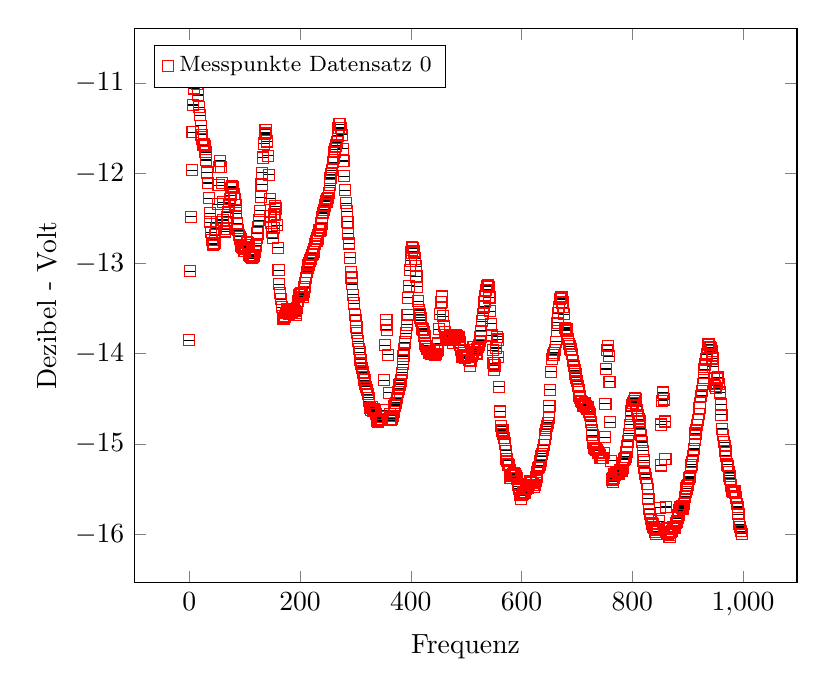
\begin{tikzpicture}
		\pgfplotsset{width=10cm,compat=1.3,legend style={font=\footnotesize}}
		\begin{axis}[xlabel={Frequenz},ylabel={Dezibel - Volt},legend cell align=left,legend pos=north west]
		
\addplot+[only marks,color=red,mark=square,error bars/.cd,x dir=both,x explicit,y dir=both,y explicit,error bar style={color=black}] table[x=X,y=Y,x error=xerror,y error=yerror,row sep=\\]{
			X	Y	xerror	yerror	\\
			 0.0 	 -13.848843 	 0 	 0 	\\
			 1.464844 	 -13.084864 	 0 	 0 	\\
			 2.929687 	 -12.482075 	 0 	 0 	\\
			 4.394531 	 -11.965661 	 0 	 0 	\\
			 5.859375 	 -11.546794 	 0 	 0 	\\
			 7.324219 	 -11.244475 	 0 	 0 	\\
			 8.789062 	 -11.060753 	 0 	 0 	\\
			 10.253906 	 -10.930851 	 0 	 0 	\\
			 11.71875 	 -10.905362 	 0 	 0 	\\
			 13.183594 	 -10.945357 	 0 	 0 	\\
			 14.648437 	 -11.015081 	 0 	 0 	\\
			 16.113281 	 -11.133686 	 0 	 0 	\\
			 17.578125 	 -11.268296 	 0 	 0 	\\
			 19.042969 	 -11.358805 	 0 	 0 	\\
			 20.507812 	 -11.472242 	 0 	 0 	\\
			 21.972656 	 -11.572217 	 0 	 0 	\\
			 23.4375 	 -11.621438 	 0 	 0 	\\
			 24.902344 	 -11.691274 	 0 	 0 	\\
			 26.367187 	 -11.680804 	 0 	 0 	\\
			 27.832031 	 -11.699508 	 0 	 0 	\\
			 29.296875 	 -11.7647 	 0 	 0 	\\
			 30.761719 	 -11.852881 	 0 	 0 	\\
			 32.226562 	 -11.99242 	 0 	 0 	\\
			 33.691406 	 -12.107867 	 0 	 0 	\\
			 35.15625 	 -12.275713 	 0 	 0 	\\
			 36.621094 	 -12.441633 	 0 	 0 	\\
			 38.085937 	 -12.54294 	 0 	 0 	\\
			 39.550781 	 -12.651932 	 0 	 0 	\\
			 41.015625 	 -12.737365 	 0 	 0 	\\
			 42.480469 	 -12.788693 	 0 	 0 	\\
			 43.945312 	 -12.777987 	 0 	 0 	\\
			 45.410156 	 -12.77724 	 0 	 0 	\\
			 46.875 	 -12.68664 	 0 	 0 	\\
			 48.339844 	 -12.616001 	 0 	 0 	\\
			 49.804687 	 -12.544291 	 0 	 0 	\\
			 51.269531 	 -12.344349 	 0 	 0 	\\
			 52.734375 	 -12.132418 	 0 	 0 	\\
			 54.199219 	 -11.929949 	 0 	 0 	\\
			 55.664062 	 -11.861673 	 0 	 0 	\\
			 57.128906 	 -11.927901 	 0 	 0 	\\
			 58.59375 	 -12.103909 	 0 	 0 	\\
			 60.058594 	 -12.32203 	 0 	 0 	\\
			 61.523437 	 -12.517847 	 0 	 0 	\\
			 62.988281 	 -12.616468 	 0 	 0 	\\
			 64.453125 	 -12.645748 	 0 	 0 	\\
			 65.917969 	 -12.61736 	 0 	 0 	\\
			 67.382812 	 -12.552704 	 0 	 0 	\\
			 68.847656 	 -12.484294 	 0 	 0 	\\
			 70.3125 	 -12.432589 	 0 	 0 	\\
			 71.777344 	 -12.339848 	 0 	 0 	\\
			 73.242187 	 -12.285835 	 0 	 0 	\\
			 74.707031 	 -12.244226 	 0 	 0 	\\
			 76.171875 	 -12.159871 	 0 	 0 	\\
			 77.636719 	 -12.146492 	 0 	 0 	\\
			 79.101562 	 -12.15427 	 0 	 0 	\\
			 80.566406 	 -12.22811 	 0 	 0 	\\
			 82.03125 	 -12.288702 	 0 	 0 	\\
			 83.496094 	 -12.357264 	 0 	 0 	\\
			 84.960937 	 -12.44275 	 0 	 0 	\\
			 86.425781 	 -12.553677 	 0 	 0 	\\
			 87.890625 	 -12.6296 	 0 	 0 	\\
			 89.355469 	 -12.688173 	 0 	 0 	\\
			 90.820312 	 -12.704946 	 0 	 0 	\\
			 92.285156 	 -12.731203 	 0 	 0 	\\
			 93.75 	 -12.801209 	 0 	 0 	\\
			 95.214844 	 -12.81376 	 0 	 0 	\\
			 96.679687 	 -12.822852 	 0 	 0 	\\
			 98.144531 	 -12.862325 	 0 	 0 	\\
			 99.609375 	 -12.835527 	 0 	 0 	\\
			 101.074219 	 -12.861899 	 0 	 0 	\\
			 102.539062 	 -12.796264 	 0 	 0 	\\
			 104.003906 	 -12.767695 	 0 	 0 	\\
			 105.46875 	 -12.776719 	 0 	 0 	\\
			 106.933594 	 -12.820479 	 0 	 0 	\\
			 108.398437 	 -12.902568 	 0 	 0 	\\
			 109.863281 	 -12.912542 	 0 	 0 	\\
			 111.328125 	 -12.925619 	 0 	 0 	\\
			 112.792969 	 -12.94205 	 0 	 0 	\\
			 114.257812 	 -12.925128 	 0 	 0 	\\
			 115.722656 	 -12.917577 	 0 	 0 	\\
			 117.1875 	 -12.910091 	 0 	 0 	\\
			 118.652344 	 -12.877029 	 0 	 0 	\\
			 120.117187 	 -12.804531 	 0 	 0 	\\
			 121.582031 	 -12.721627 	 0 	 0 	\\
			 123.046875 	 -12.667387 	 0 	 0 	\\
			 124.511719 	 -12.593013 	 0 	 0 	\\
			 125.976562 	 -12.521207 	 0 	 0 	\\
			 127.441406 	 -12.417398 	 0 	 0 	\\
			 128.90625 	 -12.265208 	 0 	 0 	\\
			 130.371094 	 -12.125359 	 0 	 0 	\\
			 131.835937 	 -11.994921 	 0 	 0 	\\
			 133.300781 	 -11.826387 	 0 	 0 	\\
			 134.765625 	 -11.671044 	 0 	 0 	\\
			 136.230469 	 -11.565237 	 0 	 0 	\\
			 137.695312 	 -11.518209 	 0 	 0 	\\
			 139.160156 	 -11.552087 	 0 	 0 	\\
			 140.625 	 -11.648033 	 0 	 0 	\\
			 142.089844 	 -11.807956 	 0 	 0 	\\
			 143.554687 	 -12.018671 	 0 	 0 	\\
			 145.019531 	 -12.281651 	 0 	 0 	\\
			 146.484375 	 -12.478611 	 0 	 0 	\\
			 147.949219 	 -12.546177 	 0 	 0 	\\
			 149.414062 	 -12.648767 	 0 	 0 	\\
			 150.878906 	 -12.717481 	 0 	 0 	\\
			 152.34375 	 -12.60883 	 0 	 0 	\\
			 153.808594 	 -12.45765 	 0 	 0 	\\
			 155.273437 	 -12.368136 	 0 	 0 	\\
			 156.738281 	 -12.391095 	 0 	 0 	\\
			 158.203125 	 -12.574885 	 0 	 0 	\\
			 159.667969 	 -12.825482 	 0 	 0 	\\
			 161.132812 	 -13.075072 	 0 	 0 	\\
			 162.597656 	 -13.229819 	 0 	 0 	\\
			 164.0625 	 -13.330846 	 0 	 0 	\\
			 165.527344 	 -13.396548 	 0 	 0 	\\
			 166.992187 	 -13.48553 	 0 	 0 	\\
			 168.457031 	 -13.585124 	 0 	 0 	\\
			 169.921875 	 -13.610015 	 0 	 0 	\\
			 171.386719 	 -13.605334 	 0 	 0 	\\
			 172.851562 	 -13.591405 	 0 	 0 	\\
			 174.316406 	 -13.544796 	 0 	 0 	\\
			 175.78125 	 -13.542664 	 0 	 0 	\\
			 177.246094 	 -13.510556 	 0 	 0 	\\
			 178.710937 	 -13.52105 	 0 	 0 	\\
			 180.175781 	 -13.553794 	 0 	 0 	\\
			 181.640625 	 -13.548846 	 0 	 0 	\\
			 183.105469 	 -13.544876 	 0 	 0 	\\
			 184.570312 	 -13.54253 	 0 	 0 	\\
			 186.035156 	 -13.513837 	 0 	 0 	\\
			 187.5 	 -13.507518 	 0 	 0 	\\
			 188.964844 	 -13.50047 	 0 	 0 	\\
			 190.429687 	 -13.527512 	 0 	 0 	\\
			 191.894531 	 -13.570786 	 0 	 0 	\\
			 193.359375 	 -13.552947 	 0 	 0 	\\
			 194.824219 	 -13.494712 	 0 	 0 	\\
			 196.289062 	 -13.41887 	 0 	 0 	\\
			 197.753906 	 -13.353909 	 0 	 0 	\\
			 199.21875 	 -13.337684 	 0 	 0 	\\
			 200.683594 	 -13.351425 	 0 	 0 	\\
			 202.148437 	 -13.330976 	 0 	 0 	\\
			 203.613281 	 -13.34627 	 0 	 0 	\\
			 205.078125 	 -13.370569 	 0 	 0 	\\
			 206.542969 	 -13.317163 	 0 	 0 	\\
			 208.007812 	 -13.262286 	 0 	 0 	\\
			 209.472656 	 -13.217603 	 0 	 0 	\\
			 210.9375 	 -13.157769 	 0 	 0 	\\
			 212.402344 	 -13.092333 	 0 	 0 	\\
			 213.867187 	 -13.048602 	 0 	 0 	\\
			 215.332031 	 -13.01314 	 0 	 0 	\\
			 216.796875 	 -12.999195 	 0 	 0 	\\
			 218.261719 	 -12.967447 	 0 	 0 	\\
			 219.726562 	 -12.943947 	 0 	 0 	\\
			 221.191406 	 -12.908824 	 0 	 0 	\\
			 222.65625 	 -12.892823 	 0 	 0 	\\
			 224.121094 	 -12.873651 	 0 	 0 	\\
			 225.585937 	 -12.845595 	 0 	 0 	\\
			 227.050781 	 -12.787115 	 0 	 0 	\\
			 228.515625 	 -12.751273 	 0 	 0 	\\
			 229.980469 	 -12.753224 	 0 	 0 	\\
			 231.445312 	 -12.723715 	 0 	 0 	\\
			 232.910156 	 -12.690077 	 0 	 0 	\\
			 234.375 	 -12.628439 	 0 	 0 	\\
			 235.839844 	 -12.634004 	 0 	 0 	\\
			 237.304687 	 -12.631191 	 0 	 0 	\\
			 238.769531 	 -12.556608 	 0 	 0 	\\
			 240.234375 	 -12.487989 	 0 	 0 	\\
			 241.699219 	 -12.44106 	 0 	 0 	\\
			 243.164062 	 -12.403562 	 0 	 0 	\\
			 244.628906 	 -12.357152 	 0 	 0 	\\
			 246.09375 	 -12.307795 	 0 	 0 	\\
			 247.558594 	 -12.317731 	 0 	 0 	\\
			 249.023437 	 -12.281264 	 0 	 0 	\\
			 250.488281 	 -12.27329 	 0 	 0 	\\
			 251.953125 	 -12.218162 	 0 	 0 	\\
			 253.417969 	 -12.134033 	 0 	 0 	\\
			 254.882812 	 -12.052472 	 0 	 0 	\\
			 256.347656 	 -12.011626 	 0 	 0 	\\
			 257.8125 	 -11.966825 	 0 	 0 	\\
			 259.277344 	 -11.878083 	 0 	 0 	\\
			 260.742187 	 -11.830478 	 0 	 0 	\\
			 262.207031 	 -11.761236 	 0 	 0 	\\
			 263.671875 	 -11.733871 	 0 	 0 	\\
			 265.136719 	 -11.693561 	 0 	 0 	\\
			 266.601562 	 -11.65706 	 0 	 0 	\\
			 268.066406 	 -11.581274 	 0 	 0 	\\
			 269.53125 	 -11.497283 	 0 	 0 	\\
			 270.996094 	 -11.455608 	 0 	 0 	\\
			 272.460937 	 -11.459285 	 0 	 0 	\\
			 273.925781 	 -11.501212 	 0 	 0 	\\
			 275.390625 	 -11.572617 	 0 	 0 	\\
			 276.855469 	 -11.727455 	 0 	 0 	\\
			 278.320312 	 -11.864044 	 0 	 0 	\\
			 279.785156 	 -12.032756 	 0 	 0 	\\
			 281.25 	 -12.188835 	 0 	 0 	\\
			 282.714844 	 -12.331757 	 0 	 0 	\\
			 284.179687 	 -12.420208 	 0 	 0 	\\
			 285.644531 	 -12.53871 	 0 	 0 	\\
			 287.109375 	 -12.671718 	 0 	 0 	\\
			 288.574219 	 -12.778358 	 0 	 0 	\\
			 290.039062 	 -12.93537 	 0 	 0 	\\
			 291.503906 	 -13.090729 	 0 	 0 	\\
			 292.96875 	 -13.155254 	 0 	 0 	\\
			 294.433594 	 -13.231764 	 0 	 0 	\\
			 295.898437 	 -13.346051 	 0 	 0 	\\
			 297.363281 	 -13.442986 	 0 	 0 	\\
			 298.828125 	 -13.570926 	 0 	 0 	\\
			 300.292969 	 -13.628228 	 0 	 0 	\\
			 301.757812 	 -13.707827 	 0 	 0 	\\
			 303.222656 	 -13.771672 	 0 	 0 	\\
			 304.6875 	 -13.86243 	 0 	 0 	\\
			 306.152344 	 -13.943918 	 0 	 0 	\\
			 307.617187 	 -13.982186 	 0 	 0 	\\
			 309.082031 	 -14.064806 	 0 	 0 	\\
			 310.546875 	 -14.108041 	 0 	 0 	\\
			 312.011719 	 -14.155785 	 0 	 0 	\\
			 313.476562 	 -14.207383 	 0 	 0 	\\
			 314.941406 	 -14.259609 	 0 	 0 	\\
			 316.40625 	 -14.295196 	 0 	 0 	\\
			 317.871094 	 -14.331971 	 0 	 0 	\\
			 319.335937 	 -14.366945 	 0 	 0 	\\
			 320.800781 	 -14.399659 	 0 	 0 	\\
			 322.265625 	 -14.448483 	 0 	 0 	\\
			 323.730469 	 -14.488628 	 0 	 0 	\\
			 325.195312 	 -14.527894 	 0 	 0 	\\
			 326.660156 	 -14.602149 	 0 	 0 	\\
			 328.125 	 -14.620625 	 0 	 0 	\\
			 329.589844 	 -14.593219 	 0 	 0 	\\
			 331.054687 	 -14.630564 	 0 	 0 	\\
			 332.519531 	 -14.630167 	 0 	 0 	\\
			 333.984375 	 -14.608939 	 0 	 0 	\\
			 335.449219 	 -14.636128 	 0 	 0 	\\
			 336.914062 	 -14.667382 	 0 	 0 	\\
			 338.378906 	 -14.725865 	 0 	 0 	\\
			 339.84375 	 -14.742405 	 0 	 0 	\\
			 341.308594 	 -14.755925 	 0 	 0 	\\
			 342.773437 	 -14.733687 	 0 	 0 	\\
			 344.238281 	 -14.720973 	 0 	 0 	\\
			 345.703125 	 -14.734243 	 0 	 0 	\\
			 347.167969 	 -14.721421 	 0 	 0 	\\
			 348.632812 	 -14.700672 	 0 	 0 	\\
			 350.097656 	 -14.624208 	 0 	 0 	\\
			 351.5625 	 -14.293939 	 0 	 0 	\\
			 353.027344 	 -13.905712 	 0 	 0 	\\
			 354.492187 	 -13.677462 	 0 	 0 	\\
			 355.957031 	 -13.621806 	 0 	 0 	\\
			 357.421875 	 -13.733462 	 0 	 0 	\\
			 358.886719 	 -14.009808 	 0 	 0 	\\
			 360.351562 	 -14.433584 	 0 	 0 	\\
			 361.816406 	 -14.665124 	 0 	 0 	\\
			 363.28125 	 -14.717876 	 0 	 0 	\\
			 364.746094 	 -14.737621 	 0 	 0 	\\
			 366.210937 	 -14.718402 	 0 	 0 	\\
			 367.675781 	 -14.686362 	 0 	 0 	\\
			 369.140625 	 -14.64979 	 0 	 0 	\\
			 370.605469 	 -14.578752 	 0 	 0 	\\
			 372.070312 	 -14.563558 	 0 	 0 	\\
			 373.535156 	 -14.541807 	 0 	 0 	\\
			 375.0 	 -14.491673 	 0 	 0 	\\
			 376.464844 	 -14.426708 	 0 	 0 	\\
			 377.929687 	 -14.385033 	 0 	 0 	\\
			 379.394531 	 -14.344742 	 0 	 0 	\\
			 380.859375 	 -14.338758 	 0 	 0 	\\
			 382.324219 	 -14.297165 	 0 	 0 	\\
			 383.789062 	 -14.21249 	 0 	 0 	\\
			 385.253906 	 -14.117258 	 0 	 0 	\\
			 386.71875 	 -14.024889 	 0 	 0 	\\
			 388.183594 	 -13.94739 	 0 	 0 	\\
			 389.648437 	 -13.874926 	 0 	 0 	\\
			 391.113281 	 -13.773478 	 0 	 0 	\\
			 392.578125 	 -13.67769 	 0 	 0 	\\
			 394.042969 	 -13.566935 	 0 	 0 	\\
			 395.507812 	 -13.380635 	 0 	 0 	\\
			 396.972656 	 -13.246249 	 0 	 0 	\\
			 398.4375 	 -13.075774 	 0 	 0 	\\
			 399.902344 	 -12.971014 	 0 	 0 	\\
			 401.367187 	 -12.878876 	 0 	 0 	\\
			 402.832031 	 -12.8139 	 0 	 0 	\\
			 404.296875 	 -12.828142 	 0 	 0 	\\
			 405.761719 	 -12.866463 	 0 	 0 	\\
			 407.226562 	 -12.945724 	 0 	 0 	\\
			 408.691406 	 -13.031688 	 0 	 0 	\\
			 410.15625 	 -13.14485 	 0 	 0 	\\
			 411.621094 	 -13.257695 	 0 	 0 	\\
			 413.085937 	 -13.418539 	 0 	 0 	\\
			 414.550781 	 -13.515303 	 0 	 0 	\\
			 416.015625 	 -13.560336 	 0 	 0 	\\
			 417.480469 	 -13.602901 	 0 	 0 	\\
			 418.945312 	 -13.633774 	 0 	 0 	\\
			 420.410156 	 -13.721082 	 0 	 0 	\\
			 421.875 	 -13.732183 	 0 	 0 	\\
			 423.339844 	 -13.758321 	 0 	 0 	\\
			 424.804687 	 -13.801134 	 0 	 0 	\\
			 426.269531 	 -13.888743 	 0 	 0 	\\
			 427.734375 	 -13.913864 	 0 	 0 	\\
			 429.199219 	 -13.943489 	 0 	 0 	\\
			 430.664062 	 -13.944173 	 0 	 0 	\\
			 432.128906 	 -13.951193 	 0 	 0 	\\
			 433.59375 	 -13.988607 	 0 	 0 	\\
			 435.058594 	 -13.984307 	 0 	 0 	\\
			 436.523437 	 -14.003439 	 0 	 0 	\\
			 437.988281 	 -14.003711 	 0 	 0 	\\
			 439.453125 	 -14.003144 	 0 	 0 	\\
			 440.917969 	 -13.999819 	 0 	 0 	\\
			 442.382812 	 -13.974069 	 0 	 0 	\\
			 443.847656 	 -14.010213 	 0 	 0 	\\
			 445.3125 	 -14.005608 	 0 	 0 	\\
			 446.777344 	 -13.972788 	 0 	 0 	\\
			 448.242187 	 -13.957638 	 0 	 0 	\\
			 449.707031 	 -13.886552 	 0 	 0 	\\
			 451.171875 	 -13.726927 	 0 	 0 	\\
			 452.636719 	 -13.564186 	 0 	 0 	\\
			 454.101562 	 -13.431608 	 0 	 0 	\\
			 455.566406 	 -13.365859 	 0 	 0 	\\
			 457.03125 	 -13.423494 	 0 	 0 	\\
			 458.496094 	 -13.582422 	 0 	 0 	\\
			 459.960937 	 -13.695712 	 0 	 0 	\\
			 461.425781 	 -13.759894 	 0 	 0 	\\
			 462.890625 	 -13.793842 	 0 	 0 	\\
			 464.355469 	 -13.827708 	 0 	 0 	\\
			 465.820312 	 -13.83685 	 0 	 0 	\\
			 467.285156 	 -13.830297 	 0 	 0 	\\
			 468.75 	 -13.81644 	 0 	 0 	\\
			 470.214844 	 -13.845641 	 0 	 0 	\\
			 471.679687 	 -13.829206 	 0 	 0 	\\
			 473.144531 	 -13.803917 	 0 	 0 	\\
			 474.609375 	 -13.849516 	 0 	 0 	\\
			 476.074219 	 -13.880946 	 0 	 0 	\\
			 477.539062 	 -13.848585 	 0 	 0 	\\
			 479.003906 	 -13.831017 	 0 	 0 	\\
			 480.46875 	 -13.805676 	 0 	 0 	\\
			 481.933594 	 -13.791267 	 0 	 0 	\\
			 483.398437 	 -13.800226 	 0 	 0 	\\
			 484.863281 	 -13.818996 	 0 	 0 	\\
			 486.328125 	 -13.818732 	 0 	 0 	\\
			 487.792969 	 -13.86874 	 0 	 0 	\\
			 489.257812 	 -13.907663 	 0 	 0 	\\
			 490.722656 	 -13.961497 	 0 	 0 	\\
			 492.1875 	 -14.02978 	 0 	 0 	\\
			 493.652344 	 -14.019824 	 0 	 0 	\\
			 495.117187 	 -14.010858 	 0 	 0 	\\
			 496.582031 	 -14.030786 	 0 	 0 	\\
			 498.046875 	 -14.049811 	 0 	 0 	\\
			 499.511719 	 -14.020986 	 0 	 0 	\\
			 500.976562 	 -14.028292 	 0 	 0 	\\
			 502.441406 	 -14.02857 	 0 	 0 	\\
			 503.90625 	 -14.038276 	 0 	 0 	\\
			 505.371094 	 -14.073226 	 0 	 0 	\\
			 506.835937 	 -14.139538 	 0 	 0 	\\
			 508.300781 	 -14.082113 	 0 	 0 	\\
			 509.765625 	 -14.022043 	 0 	 0 	\\
			 511.230469 	 -13.977014 	 0 	 0 	\\
			 512.695312 	 -13.928044 	 0 	 0 	\\
			 514.160156 	 -13.927798 	 0 	 0 	\\
			 515.625 	 -13.961398 	 0 	 0 	\\
			 517.089844 	 -13.9973 	 0 	 0 	\\
			 518.554687 	 -14.001409 	 0 	 0 	\\
			 520.019531 	 -13.952327 	 0 	 0 	\\
			 521.484375 	 -13.921497 	 0 	 0 	\\
			 522.949219 	 -13.899399 	 0 	 0 	\\
			 524.414062 	 -13.856237 	 0 	 0 	\\
			 525.878906 	 -13.811698 	 0 	 0 	\\
			 527.34375 	 -13.74543 	 0 	 0 	\\
			 528.808594 	 -13.640151 	 0 	 0 	\\
			 530.273437 	 -13.558892 	 0 	 0 	\\
			 531.738281 	 -13.476128 	 0 	 0 	\\
			 533.203125 	 -13.424129 	 0 	 0 	\\
			 534.667969 	 -13.361391 	 0 	 0 	\\
			 536.132812 	 -13.290147 	 0 	 0 	\\
			 537.597656 	 -13.249411 	 0 	 0 	\\
			 539.0625 	 -13.243973 	 0 	 0 	\\
			 540.527344 	 -13.258794 	 0 	 0 	\\
			 541.992187 	 -13.376017 	 0 	 0 	\\
			 543.457031 	 -13.53083 	 0 	 0 	\\
			 544.921875 	 -13.669553 	 0 	 0 	\\
			 546.386719 	 -13.797888 	 0 	 0 	\\
			 547.851562 	 -13.962575 	 0 	 0 	\\
			 549.316406 	 -14.103863 	 0 	 0 	\\
			 550.78125 	 -14.175672 	 0 	 0 	\\
			 552.246094 	 -14.129969 	 0 	 0 	\\
			 553.710937 	 -13.935889 	 0 	 0 	\\
			 555.175781 	 -13.812741 	 0 	 0 	\\
			 556.640625 	 -13.842486 	 0 	 0 	\\
			 558.105469 	 -14.0394 	 0 	 0 	\\
			 559.570312 	 -14.36572 	 0 	 0 	\\
			 561.035156 	 -14.639869 	 0 	 0 	\\
			 562.5 	 -14.803625 	 0 	 0 	\\
			 563.964844 	 -14.852777 	 0 	 0 	\\
			 565.429687 	 -14.841215 	 0 	 0 	\\
			 566.894531 	 -14.885598 	 0 	 0 	\\
			 568.359375 	 -14.93465 	 0 	 0 	\\
			 569.824219 	 -14.995193 	 0 	 0 	\\
			 571.289062 	 -15.075983 	 0 	 0 	\\
			 572.753906 	 -15.162594 	 0 	 0 	\\
			 574.21875 	 -15.184264 	 0 	 0 	\\
			 575.683594 	 -15.227345 	 0 	 0 	\\
			 577.148437 	 -15.232505 	 0 	 0 	\\
			 578.613281 	 -15.293614 	 0 	 0 	\\
			 580.078125 	 -15.372789 	 0 	 0 	\\
			 581.542969 	 -15.356886 	 0 	 0 	\\
			 583.007812 	 -15.342438 	 0 	 0 	\\
			 584.472656 	 -15.331652 	 0 	 0 	\\
			 585.9375 	 -15.325742 	 0 	 0 	\\
			 587.402344 	 -15.342131 	 0 	 0 	\\
			 588.867187 	 -15.331516 	 0 	 0 	\\
			 590.332031 	 -15.355327 	 0 	 0 	\\
			 591.796875 	 -15.381597 	 0 	 0 	\\
			 593.261719 	 -15.448496 	 0 	 0 	\\
			 594.726562 	 -15.472652 	 0 	 0 	\\
			 596.191406 	 -15.492994 	 0 	 0 	\\
			 597.65625 	 -15.566356 	 0 	 0 	\\
			 599.121094 	 -15.605995 	 0 	 0 	\\
			 600.585937 	 -15.568733 	 0 	 0 	\\
			 602.050781 	 -15.554772 	 0 	 0 	\\
			 603.515625 	 -15.53828 	 0 	 0 	\\
			 604.980469 	 -15.538965 	 0 	 0 	\\
			 606.445312 	 -15.536983 	 0 	 0 	\\
			 607.910156 	 -15.502813 	 0 	 0 	\\
			 609.375 	 -15.469022 	 0 	 0 	\\
			 610.839844 	 -15.483412 	 0 	 0 	\\
			 612.304687 	 -15.461215 	 0 	 0 	\\
			 613.769531 	 -15.456343 	 0 	 0 	\\
			 615.234375 	 -15.407683 	 0 	 0 	\\
			 616.699219 	 -15.420788 	 0 	 0 	\\
			 618.164062 	 -15.43605 	 0 	 0 	\\
			 619.628906 	 -15.432121 	 0 	 0 	\\
			 621.09375 	 -15.455558 	 0 	 0 	\\
			 622.558594 	 -15.478613 	 0 	 0 	\\
			 624.023437 	 -15.449878 	 0 	 0 	\\
			 625.488281 	 -15.404584 	 0 	 0 	\\
			 626.953125 	 -15.368659 	 0 	 0 	\\
			 628.417969 	 -15.307146 	 0 	 0 	\\
			 629.882812 	 -15.26498 	 0 	 0 	\\
			 631.347656 	 -15.254311 	 0 	 0 	\\
			 632.8125 	 -15.235234 	 0 	 0 	\\
			 634.277344 	 -15.186217 	 0 	 0 	\\
			 635.742187 	 -15.138761 	 0 	 0 	\\
			 637.207031 	 -15.106788 	 0 	 0 	\\
			 638.671875 	 -15.069259 	 0 	 0 	\\
			 640.136719 	 -15.015678 	 0 	 0 	\\
			 641.601562 	 -14.946323 	 0 	 0 	\\
			 643.066406 	 -14.888166 	 0 	 0 	\\
			 644.53125 	 -14.841577 	 0 	 0 	\\
			 645.996094 	 -14.80279 	 0 	 0 	\\
			 647.460937 	 -14.763057 	 0 	 0 	\\
			 648.925781 	 -14.707606 	 0 	 0 	\\
			 650.390625 	 -14.576478 	 0 	 0 	\\
			 651.855469 	 -14.399101 	 0 	 0 	\\
			 653.320312 	 -14.201233 	 0 	 0 	\\
			 654.785156 	 -14.05587 	 0 	 0 	\\
			 656.25 	 -14.01161 	 0 	 0 	\\
			 657.714844 	 -14.015326 	 0 	 0 	\\
			 659.179687 	 -13.989563 	 0 	 0 	\\
			 660.644531 	 -13.957742 	 0 	 0 	\\
			 662.109375 	 -13.86798 	 0 	 0 	\\
			 663.574219 	 -13.74568 	 0 	 0 	\\
			 665.039062 	 -13.655993 	 0 	 0 	\\
			 666.503906 	 -13.551404 	 0 	 0 	\\
			 667.96875 	 -13.482943 	 0 	 0 	\\
			 669.433594 	 -13.394012 	 0 	 0 	\\
			 670.898437 	 -13.376683 	 0 	 0 	\\
			 672.363281 	 -13.373598 	 0 	 0 	\\
			 673.828125 	 -13.432512 	 0 	 0 	\\
			 675.292969 	 -13.483224 	 0 	 0 	\\
			 676.757812 	 -13.563242 	 0 	 0 	\\
			 678.222656 	 -13.713531 	 0 	 0 	\\
			 679.6875 	 -13.731859 	 0 	 0 	\\
			 681.152344 	 -13.725105 	 0 	 0 	\\
			 682.617187 	 -13.746216 	 0 	 0 	\\
			 684.082031 	 -13.834937 	 0 	 0 	\\
			 685.546875 	 -13.892766 	 0 	 0 	\\
			 687.011719 	 -13.917761 	 0 	 0 	\\
			 688.476562 	 -13.944634 	 0 	 0 	\\
			 689.941406 	 -13.954781 	 0 	 0 	\\
			 691.40625 	 -14.00583 	 0 	 0 	\\
			 692.871094 	 -14.080033 	 0 	 0 	\\
			 694.335937 	 -14.13577 	 0 	 0 	\\
			 695.800781 	 -14.186631 	 0 	 0 	\\
			 697.265625 	 -14.221995 	 0 	 0 	\\
			 698.730469 	 -14.264764 	 0 	 0 	\\
			 700.195312 	 -14.304014 	 0 	 0 	\\
			 701.660156 	 -14.358989 	 0 	 0 	\\
			 703.125 	 -14.406108 	 0 	 0 	\\
			 704.589844 	 -14.467628 	 0 	 0 	\\
			 706.054687 	 -14.492406 	 0 	 0 	\\
			 707.519531 	 -14.52735 	 0 	 0 	\\
			 708.984375 	 -14.533796 	 0 	 0 	\\
			 710.449219 	 -14.557829 	 0 	 0 	\\
			 711.914062 	 -14.576191 	 0 	 0 	\\
			 713.378906 	 -14.564985 	 0 	 0 	\\
			 714.84375 	 -14.551908 	 0 	 0 	\\
			 716.308594 	 -14.585457 	 0 	 0 	\\
			 717.773437 	 -14.60963 	 0 	 0 	\\
			 719.238281 	 -14.594293 	 0 	 0 	\\
			 720.703125 	 -14.598125 	 0 	 0 	\\
			 722.167969 	 -14.644541 	 0 	 0 	\\
			 723.632812 	 -14.672808 	 0 	 0 	\\
			 725.097656 	 -14.752396 	 0 	 0 	\\
			 726.5625 	 -14.851145 	 0 	 0 	\\
			 728.027344 	 -14.90107 	 0 	 0 	\\
			 729.492187 	 -14.983686 	 0 	 0 	\\
			 730.957031 	 -15.045944 	 0 	 0 	\\
			 732.421875 	 -15.059546 	 0 	 0 	\\
			 733.886719 	 -15.05426 	 0 	 0 	\\
			 735.351562 	 -15.064187 	 0 	 0 	\\
			 736.816406 	 -15.066898 	 0 	 0 	\\
			 738.28125 	 -15.093438 	 0 	 0 	\\
			 739.746094 	 -15.100656 	 0 	 0 	\\
			 741.210937 	 -15.12522 	 0 	 0 	\\
			 742.675781 	 -15.158319 	 0 	 0 	\\
			 744.140625 	 -15.157933 	 0 	 0 	\\
			 745.605469 	 -15.158154 	 0 	 0 	\\
			 747.070312 	 -15.158847 	 0 	 0 	\\
			 748.535156 	 -15.099766 	 0 	 0 	\\
			 750.0 	 -14.92643 	 0 	 0 	\\
			 751.464844 	 -14.552396 	 0 	 0 	\\
			 752.929687 	 -14.1692 	 0 	 0 	\\
			 754.394531 	 -13.958285 	 0 	 0 	\\
			 755.859375 	 -13.911774 	 0 	 0 	\\
			 757.324219 	 -14.028664 	 0 	 0 	\\
			 758.789062 	 -14.312077 	 0 	 0 	\\
			 760.253906 	 -14.760731 	 0 	 0 	\\
			 761.71875 	 -15.184678 	 0 	 0 	\\
			 763.183594 	 -15.392624 	 0 	 0 	\\
			 764.648437 	 -15.418165 	 0 	 0 	\\
			 766.113281 	 -15.377866 	 0 	 0 	\\
			 767.578125 	 -15.336439 	 0 	 0 	\\
			 769.042969 	 -15.34766 	 0 	 0 	\\
			 770.507812 	 -15.309141 	 0 	 0 	\\
			 771.972656 	 -15.309903 	 0 	 0 	\\
			 773.4375 	 -15.321543 	 0 	 0 	\\
			 774.902344 	 -15.330109 	 0 	 0 	\\
			 776.367187 	 -15.306724 	 0 	 0 	\\
			 777.832031 	 -15.288806 	 0 	 0 	\\
			 779.296875 	 -15.301909 	 0 	 0 	\\
			 780.761719 	 -15.295229 	 0 	 0 	\\
			 782.226562 	 -15.27009 	 0 	 0 	\\
			 783.691406 	 -15.208692 	 0 	 0 	\\
			 785.15625 	 -15.171063 	 0 	 0 	\\
			 786.621094 	 -15.161349 	 0 	 0 	\\
			 788.085937 	 -15.1401 	 0 	 0 	\\
			 789.550781 	 -15.091379 	 0 	 0 	\\
			 791.015625 	 -15.026564 	 0 	 0 	\\
			 792.480469 	 -14.972059 	 0 	 0 	\\
			 793.945312 	 -14.887531 	 0 	 0 	\\
			 795.410156 	 -14.786565 	 0 	 0 	\\
			 796.875 	 -14.689001 	 0 	 0 	\\
			 798.339844 	 -14.635184 	 0 	 0 	\\
			 799.804687 	 -14.567341 	 0 	 0 	\\
			 801.269531 	 -14.541805 	 0 	 0 	\\
			 802.734375 	 -14.523753 	 0 	 0 	\\
			 804.199219 	 -14.48997 	 0 	 0 	\\
			 805.664062 	 -14.504683 	 0 	 0 	\\
			 807.128906 	 -14.57874 	 0 	 0 	\\
			 808.59375 	 -14.629734 	 0 	 0 	\\
			 810.058594 	 -14.684223 	 0 	 0 	\\
			 811.523437 	 -14.72411 	 0 	 0 	\\
			 812.988281 	 -14.750403 	 0 	 0 	\\
			 814.453125 	 -14.831126 	 0 	 0 	\\
			 815.917969 	 -14.904781 	 0 	 0 	\\
			 817.382812 	 -14.977625 	 0 	 0 	\\
			 818.847656 	 -15.07545 	 0 	 0 	\\
			 820.3125 	 -15.182081 	 0 	 0 	\\
			 821.777344 	 -15.261506 	 0 	 0 	\\
			 823.242187 	 -15.335604 	 0 	 0 	\\
			 824.707031 	 -15.375717 	 0 	 0 	\\
			 826.171875 	 -15.442172 	 0 	 0 	\\
			 827.636719 	 -15.500808 	 0 	 0 	\\
			 829.101562 	 -15.608633 	 0 	 0 	\\
			 830.566406 	 -15.724411 	 0 	 0 	\\
			 832.03125 	 -15.778374 	 0 	 0 	\\
			 833.496094 	 -15.832983 	 0 	 0 	\\
			 834.960937 	 -15.881127 	 0 	 0 	\\
			 836.425781 	 -15.888403 	 0 	 0 	\\
			 837.890625 	 -15.916879 	 0 	 0 	\\
			 839.355469 	 -15.93463 	 0 	 0 	\\
			 840.820312 	 -15.969865 	 0 	 0 	\\
			 842.285156 	 -15.994647 	 0 	 0 	\\
			 843.75 	 -15.943043 	 0 	 0 	\\
			 845.214844 	 -15.950734 	 0 	 0 	\\
			 846.679687 	 -15.938186 	 0 	 0 	\\
			 848.144531 	 -15.857123 	 0 	 0 	\\
			 849.609375 	 -15.706494 	 0 	 0 	\\
			 851.074219 	 -15.237861 	 0 	 0 	\\
			 852.539062 	 -14.784414 	 0 	 0 	\\
			 854.003906 	 -14.521018 	 0 	 0 	\\
			 855.46875 	 -14.430327 	 0 	 0 	\\
			 856.933594 	 -14.506615 	 0 	 0 	\\
			 858.398437 	 -14.750749 	 0 	 0 	\\
			 859.863281 	 -15.167859 	 0 	 0 	\\
			 861.328125 	 -15.698378 	 0 	 0 	\\
			 862.792969 	 -15.937158 	 0 	 0 	\\
			 864.257812 	 -15.996637 	 0 	 0 	\\
			 865.722656 	 -15.98979 	 0 	 0 	\\
			 867.1875 	 -16.026136 	 0 	 0 	\\
			 868.652344 	 -16.006728 	 0 	 0 	\\
			 870.117187 	 -15.977865 	 0 	 0 	\\
			 871.582031 	 -15.966749 	 0 	 0 	\\
			 873.046875 	 -15.923391 	 0 	 0 	\\
			 874.511719 	 -15.932359 	 0 	 0 	\\
			 875.976562 	 -15.931909 	 0 	 0 	\\
			 877.441406 	 -15.925212 	 0 	 0 	\\
			 878.90625 	 -15.876147 	 0 	 0 	\\
			 880.371094 	 -15.858563 	 0 	 0 	\\
			 881.835937 	 -15.824195 	 0 	 0 	\\
			 883.300781 	 -15.790751 	 0 	 0 	\\
			 884.765625 	 -15.73282 	 0 	 0 	\\
			 886.230469 	 -15.697337 	 0 	 0 	\\
			 887.695312 	 -15.69995 	 0 	 0 	\\
			 889.160156 	 -15.708749 	 0 	 0 	\\
			 890.625 	 -15.686311 	 0 	 0 	\\
			 892.089844 	 -15.716433 	 0 	 0 	\\
			 893.554687 	 -15.665769 	 0 	 0 	\\
			 895.019531 	 -15.583663 	 0 	 0 	\\
			 896.484375 	 -15.531006 	 0 	 0 	\\
			 897.949219 	 -15.492765 	 0 	 0 	\\
			 899.414062 	 -15.469691 	 0 	 0 	\\
			 900.878906 	 -15.453538 	 0 	 0 	\\
			 902.34375 	 -15.382501 	 0 	 0 	\\
			 903.808594 	 -15.366147 	 0 	 0 	\\
			 905.273437 	 -15.253802 	 0 	 0 	\\
			 906.738281 	 -15.228529 	 0 	 0 	\\
			 908.203125 	 -15.194991 	 0 	 0 	\\
			 909.667969 	 -15.130339 	 0 	 0 	\\
			 911.132812 	 -15.055083 	 0 	 0 	\\
			 912.597656 	 -14.951272 	 0 	 0 	\\
			 914.0625 	 -14.883529 	 0 	 0 	\\
			 915.527344 	 -14.843739 	 0 	 0 	\\
			 916.992187 	 -14.787547 	 0 	 0 	\\
			 918.457031 	 -14.732906 	 0 	 0 	\\
			 919.921875 	 -14.671104 	 0 	 0 	\\
			 921.386719 	 -14.602968 	 0 	 0 	\\
			 922.851562 	 -14.544416 	 0 	 0 	\\
			 924.316406 	 -14.465856 	 0 	 0 	\\
			 925.78125 	 -14.417382 	 0 	 0 	\\
			 927.246094 	 -14.333243 	 0 	 0 	\\
			 928.710937 	 -14.265049 	 0 	 0 	\\
			 930.175781 	 -14.173132 	 0 	 0 	\\
			 931.640625 	 -14.11998 	 0 	 0 	\\
			 933.105469 	 -14.063228 	 0 	 0 	\\
			 934.570312 	 -14.009239 	 0 	 0 	\\
			 936.035156 	 -13.929794 	 0 	 0 	\\
			 937.5 	 -13.897684 	 0 	 0 	\\
			 938.964844 	 -13.903076 	 0 	 0 	\\
			 940.429687 	 -13.92639 	 0 	 0 	\\
			 941.894531 	 -13.938956 	 0 	 0 	\\
			 943.359375 	 -13.970751 	 0 	 0 	\\
			 944.824219 	 -14.052549 	 0 	 0 	\\
			 946.289062 	 -14.14161 	 0 	 0 	\\
			 947.753906 	 -14.280235 	 0 	 0 	\\
			 949.21875 	 -14.35463 	 0 	 0 	\\
			 950.683594 	 -14.382016 	 0 	 0 	\\
			 952.148437 	 -14.339008 	 0 	 0 	\\
			 953.613281 	 -14.279057 	 0 	 0 	\\
			 955.078125 	 -14.263344 	 0 	 0 	\\
			 956.542969 	 -14.334046 	 0 	 0 	\\
			 958.007812 	 -14.429471 	 0 	 0 	\\
			 959.472656 	 -14.562532 	 0 	 0 	\\
			 960.9375 	 -14.677482 	 0 	 0 	\\
			 962.402344 	 -14.83028 	 0 	 0 	\\
			 963.867187 	 -14.898317 	 0 	 0 	\\
			 965.332031 	 -14.979098 	 0 	 0 	\\
			 966.796875 	 -15.024695 	 0 	 0 	\\
			 968.261719 	 -15.074795 	 0 	 0 	\\
			 969.726562 	 -15.131465 	 0 	 0 	\\
			 971.191406 	 -15.228137 	 0 	 0 	\\
			 972.65625 	 -15.246065 	 0 	 0 	\\
			 974.121094 	 -15.310705 	 0 	 0 	\\
			 975.585937 	 -15.35391 	 0 	 0 	\\
			 977.050781 	 -15.386969 	 0 	 0 	\\
			 978.515625 	 -15.458913 	 0 	 0 	\\
			 979.980469 	 -15.517785 	 0 	 0 	\\
			 981.445312 	 -15.534356 	 0 	 0 	\\
			 982.910156 	 -15.536297 	 0 	 0 	\\
			 984.375 	 -15.525312 	 0 	 0 	\\
			 985.839844 	 -15.541296 	 0 	 0 	\\
			 987.304687 	 -15.5928 	 0 	 0 	\\
			 988.769531 	 -15.661136 	 0 	 0 	\\
			 990.234375 	 -15.698563 	 0 	 0 	\\
			 991.699219 	 -15.777128 	 0 	 0 	\\
			 993.164062 	 -15.890349 	 0 	 0 	\\
			 994.628906 	 -15.919824 	 0 	 0 	\\
			 996.09375 	 -15.968122 	 0 	 0 	\\
			 997.558594 	 -15.994696 	 0 	 0 	\\
		};
		\addlegendentry{Messpunkte Datensatz 0}

		\end{axis}
		\end{tikzpicture}
	\caption{Umgebung}
	\label{fig:Umgebungsmessung}
\end{figure}

        % \begin{figure}[H]

	\centering
	\begin{tikzpicture}
		\pgfplotsset{width=10cm,compat=1.3,legend style={font=\footnotesize}}
		\begin{axis}[xlabel={Frequenz},ylabel={Dezibel - Volt},legend cell align=left,legend pos=north west]
		
\addplot+[only marks,color=red,mark=square,error bars/.cd,x dir=both,x explicit,y dir=both,y explicit,error bar style={color=black}] table[x=X,y=Y,x error=xerror,y error=yerror,row sep=\\]{
			X	Y	xerror	yerror	\\
			 13.183594 	 -10.945357 	 0 	 0 	\\
			 55.664062 	 -11.861673 	 0 	 0 	\\
			 77.636719 	 -12.146492 	 0 	 0 	\\
			 139.160156 	 -11.552087 	 0 	 0 	\\
			 269.53125 	 -11.497283 	 0 	 0 	\\
			 357.421875 	 -13.733462 	 0 	 0 	\\
			 404.296875 	 -12.828142 	 0 	 0 	\\
			 455.566406 	 -13.365859 	 0 	 0 	\\
			 536.132812 	 -13.290147 	 0 	 0 	\\
			 672.363281 	 -13.373598 	 0 	 0 	\\
			 757.324219 	 -14.028664 	 0 	 0 	\\
			 805.664062 	 -14.504683 	 0 	 0 	\\
			 856.933594 	 -14.506615 	 0 	 0 	\\
			 940.429687 	 -13.92639 	 0 	 0 	\\
		};
		\addlegendentry{Messpunkte Datensatz 0}

		\end{axis}
		\end{tikzpicture}
	\caption{Umgebung}
	\label{fig:Umgebungsmessung}
\end{figure}

        %% \begin{figure}[H]

	\centering
	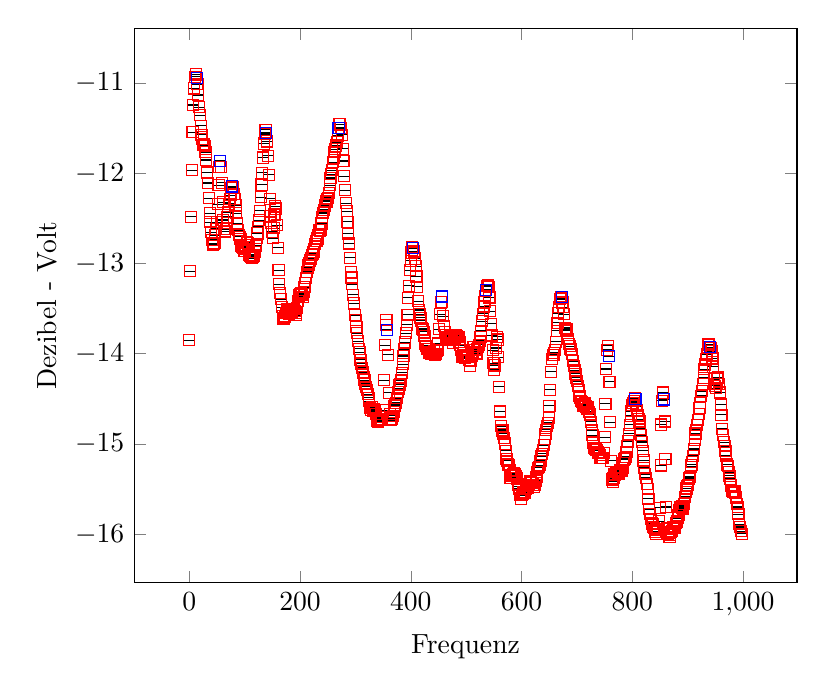
\begin{tikzpicture}
		\pgfplotsset{width=10cm,compat=1.3,legend style={font=\footnotesize}}
		\begin{axis}[xlabel={Frequenz},ylabel={Dezibel - Volt},legend cell align=left,legend pos=north west]
		
\addplot+[only marks,color=red,mark=square,error bars/.cd,x dir=both,x explicit,y dir=both,y explicit,error bar style={color=black}] table[x=X,y=Y,x error=xerror,y error=yerror,row sep=\\]{
			X	Y	xerror	yerror	\\
			 0.0 	 -13.848843 	 0 	 0 	\\
			 1.464844 	 -13.084864 	 0 	 0 	\\
			 2.929687 	 -12.482075 	 0 	 0 	\\
			 4.394531 	 -11.965661 	 0 	 0 	\\
			 5.859375 	 -11.546794 	 0 	 0 	\\
			 7.324219 	 -11.244475 	 0 	 0 	\\
			 8.789062 	 -11.060753 	 0 	 0 	\\
			 10.253906 	 -10.930851 	 0 	 0 	\\
			 11.71875 	 -10.905362 	 0 	 0 	\\
			 13.183594 	 -10.945357 	 0 	 0 	\\
			 14.648437 	 -11.015081 	 0 	 0 	\\
			 16.113281 	 -11.133686 	 0 	 0 	\\
			 17.578125 	 -11.268296 	 0 	 0 	\\
			 19.042969 	 -11.358805 	 0 	 0 	\\
			 20.507812 	 -11.472242 	 0 	 0 	\\
			 21.972656 	 -11.572217 	 0 	 0 	\\
			 23.4375 	 -11.621438 	 0 	 0 	\\
			 24.902344 	 -11.691274 	 0 	 0 	\\
			 26.367187 	 -11.680804 	 0 	 0 	\\
			 27.832031 	 -11.699508 	 0 	 0 	\\
			 29.296875 	 -11.7647 	 0 	 0 	\\
			 30.761719 	 -11.852881 	 0 	 0 	\\
			 32.226562 	 -11.99242 	 0 	 0 	\\
			 33.691406 	 -12.107867 	 0 	 0 	\\
			 35.15625 	 -12.275713 	 0 	 0 	\\
			 36.621094 	 -12.441633 	 0 	 0 	\\
			 38.085937 	 -12.54294 	 0 	 0 	\\
			 39.550781 	 -12.651932 	 0 	 0 	\\
			 41.015625 	 -12.737365 	 0 	 0 	\\
			 42.480469 	 -12.788693 	 0 	 0 	\\
			 43.945312 	 -12.777987 	 0 	 0 	\\
			 45.410156 	 -12.77724 	 0 	 0 	\\
			 46.875 	 -12.68664 	 0 	 0 	\\
			 48.339844 	 -12.616001 	 0 	 0 	\\
			 49.804687 	 -12.544291 	 0 	 0 	\\
			 51.269531 	 -12.344349 	 0 	 0 	\\
			 52.734375 	 -12.132418 	 0 	 0 	\\
			 54.199219 	 -11.929949 	 0 	 0 	\\
			 55.664062 	 -11.861673 	 0 	 0 	\\
			 57.128906 	 -11.927901 	 0 	 0 	\\
			 58.59375 	 -12.103909 	 0 	 0 	\\
			 60.058594 	 -12.32203 	 0 	 0 	\\
			 61.523437 	 -12.517847 	 0 	 0 	\\
			 62.988281 	 -12.616468 	 0 	 0 	\\
			 64.453125 	 -12.645748 	 0 	 0 	\\
			 65.917969 	 -12.61736 	 0 	 0 	\\
			 67.382812 	 -12.552704 	 0 	 0 	\\
			 68.847656 	 -12.484294 	 0 	 0 	\\
			 70.3125 	 -12.432589 	 0 	 0 	\\
			 71.777344 	 -12.339848 	 0 	 0 	\\
			 73.242187 	 -12.285835 	 0 	 0 	\\
			 74.707031 	 -12.244226 	 0 	 0 	\\
			 76.171875 	 -12.159871 	 0 	 0 	\\
			 77.636719 	 -12.146492 	 0 	 0 	\\
			 79.101562 	 -12.15427 	 0 	 0 	\\
			 80.566406 	 -12.22811 	 0 	 0 	\\
			 82.03125 	 -12.288702 	 0 	 0 	\\
			 83.496094 	 -12.357264 	 0 	 0 	\\
			 84.960937 	 -12.44275 	 0 	 0 	\\
			 86.425781 	 -12.553677 	 0 	 0 	\\
			 87.890625 	 -12.6296 	 0 	 0 	\\
			 89.355469 	 -12.688173 	 0 	 0 	\\
			 90.820312 	 -12.704946 	 0 	 0 	\\
			 92.285156 	 -12.731203 	 0 	 0 	\\
			 93.75 	 -12.801209 	 0 	 0 	\\
			 95.214844 	 -12.81376 	 0 	 0 	\\
			 96.679687 	 -12.822852 	 0 	 0 	\\
			 98.144531 	 -12.862325 	 0 	 0 	\\
			 99.609375 	 -12.835527 	 0 	 0 	\\
			 101.074219 	 -12.861899 	 0 	 0 	\\
			 102.539062 	 -12.796264 	 0 	 0 	\\
			 104.003906 	 -12.767695 	 0 	 0 	\\
			 105.46875 	 -12.776719 	 0 	 0 	\\
			 106.933594 	 -12.820479 	 0 	 0 	\\
			 108.398437 	 -12.902568 	 0 	 0 	\\
			 109.863281 	 -12.912542 	 0 	 0 	\\
			 111.328125 	 -12.925619 	 0 	 0 	\\
			 112.792969 	 -12.94205 	 0 	 0 	\\
			 114.257812 	 -12.925128 	 0 	 0 	\\
			 115.722656 	 -12.917577 	 0 	 0 	\\
			 117.1875 	 -12.910091 	 0 	 0 	\\
			 118.652344 	 -12.877029 	 0 	 0 	\\
			 120.117187 	 -12.804531 	 0 	 0 	\\
			 121.582031 	 -12.721627 	 0 	 0 	\\
			 123.046875 	 -12.667387 	 0 	 0 	\\
			 124.511719 	 -12.593013 	 0 	 0 	\\
			 125.976562 	 -12.521207 	 0 	 0 	\\
			 127.441406 	 -12.417398 	 0 	 0 	\\
			 128.90625 	 -12.265208 	 0 	 0 	\\
			 130.371094 	 -12.125359 	 0 	 0 	\\
			 131.835937 	 -11.994921 	 0 	 0 	\\
			 133.300781 	 -11.826387 	 0 	 0 	\\
			 134.765625 	 -11.671044 	 0 	 0 	\\
			 136.230469 	 -11.565237 	 0 	 0 	\\
			 137.695312 	 -11.518209 	 0 	 0 	\\
			 139.160156 	 -11.552087 	 0 	 0 	\\
			 140.625 	 -11.648033 	 0 	 0 	\\
			 142.089844 	 -11.807956 	 0 	 0 	\\
			 143.554687 	 -12.018671 	 0 	 0 	\\
			 145.019531 	 -12.281651 	 0 	 0 	\\
			 146.484375 	 -12.478611 	 0 	 0 	\\
			 147.949219 	 -12.546177 	 0 	 0 	\\
			 149.414062 	 -12.648767 	 0 	 0 	\\
			 150.878906 	 -12.717481 	 0 	 0 	\\
			 152.34375 	 -12.60883 	 0 	 0 	\\
			 153.808594 	 -12.45765 	 0 	 0 	\\
			 155.273437 	 -12.368136 	 0 	 0 	\\
			 156.738281 	 -12.391095 	 0 	 0 	\\
			 158.203125 	 -12.574885 	 0 	 0 	\\
			 159.667969 	 -12.825482 	 0 	 0 	\\
			 161.132812 	 -13.075072 	 0 	 0 	\\
			 162.597656 	 -13.229819 	 0 	 0 	\\
			 164.0625 	 -13.330846 	 0 	 0 	\\
			 165.527344 	 -13.396548 	 0 	 0 	\\
			 166.992187 	 -13.48553 	 0 	 0 	\\
			 168.457031 	 -13.585124 	 0 	 0 	\\
			 169.921875 	 -13.610015 	 0 	 0 	\\
			 171.386719 	 -13.605334 	 0 	 0 	\\
			 172.851562 	 -13.591405 	 0 	 0 	\\
			 174.316406 	 -13.544796 	 0 	 0 	\\
			 175.78125 	 -13.542664 	 0 	 0 	\\
			 177.246094 	 -13.510556 	 0 	 0 	\\
			 178.710937 	 -13.52105 	 0 	 0 	\\
			 180.175781 	 -13.553794 	 0 	 0 	\\
			 181.640625 	 -13.548846 	 0 	 0 	\\
			 183.105469 	 -13.544876 	 0 	 0 	\\
			 184.570312 	 -13.54253 	 0 	 0 	\\
			 186.035156 	 -13.513837 	 0 	 0 	\\
			 187.5 	 -13.507518 	 0 	 0 	\\
			 188.964844 	 -13.50047 	 0 	 0 	\\
			 190.429687 	 -13.527512 	 0 	 0 	\\
			 191.894531 	 -13.570786 	 0 	 0 	\\
			 193.359375 	 -13.552947 	 0 	 0 	\\
			 194.824219 	 -13.494712 	 0 	 0 	\\
			 196.289062 	 -13.41887 	 0 	 0 	\\
			 197.753906 	 -13.353909 	 0 	 0 	\\
			 199.21875 	 -13.337684 	 0 	 0 	\\
			 200.683594 	 -13.351425 	 0 	 0 	\\
			 202.148437 	 -13.330976 	 0 	 0 	\\
			 203.613281 	 -13.34627 	 0 	 0 	\\
			 205.078125 	 -13.370569 	 0 	 0 	\\
			 206.542969 	 -13.317163 	 0 	 0 	\\
			 208.007812 	 -13.262286 	 0 	 0 	\\
			 209.472656 	 -13.217603 	 0 	 0 	\\
			 210.9375 	 -13.157769 	 0 	 0 	\\
			 212.402344 	 -13.092333 	 0 	 0 	\\
			 213.867187 	 -13.048602 	 0 	 0 	\\
			 215.332031 	 -13.01314 	 0 	 0 	\\
			 216.796875 	 -12.999195 	 0 	 0 	\\
			 218.261719 	 -12.967447 	 0 	 0 	\\
			 219.726562 	 -12.943947 	 0 	 0 	\\
			 221.191406 	 -12.908824 	 0 	 0 	\\
			 222.65625 	 -12.892823 	 0 	 0 	\\
			 224.121094 	 -12.873651 	 0 	 0 	\\
			 225.585937 	 -12.845595 	 0 	 0 	\\
			 227.050781 	 -12.787115 	 0 	 0 	\\
			 228.515625 	 -12.751273 	 0 	 0 	\\
			 229.980469 	 -12.753224 	 0 	 0 	\\
			 231.445312 	 -12.723715 	 0 	 0 	\\
			 232.910156 	 -12.690077 	 0 	 0 	\\
			 234.375 	 -12.628439 	 0 	 0 	\\
			 235.839844 	 -12.634004 	 0 	 0 	\\
			 237.304687 	 -12.631191 	 0 	 0 	\\
			 238.769531 	 -12.556608 	 0 	 0 	\\
			 240.234375 	 -12.487989 	 0 	 0 	\\
			 241.699219 	 -12.44106 	 0 	 0 	\\
			 243.164062 	 -12.403562 	 0 	 0 	\\
			 244.628906 	 -12.357152 	 0 	 0 	\\
			 246.09375 	 -12.307795 	 0 	 0 	\\
			 247.558594 	 -12.317731 	 0 	 0 	\\
			 249.023437 	 -12.281264 	 0 	 0 	\\
			 250.488281 	 -12.27329 	 0 	 0 	\\
			 251.953125 	 -12.218162 	 0 	 0 	\\
			 253.417969 	 -12.134033 	 0 	 0 	\\
			 254.882812 	 -12.052472 	 0 	 0 	\\
			 256.347656 	 -12.011626 	 0 	 0 	\\
			 257.8125 	 -11.966825 	 0 	 0 	\\
			 259.277344 	 -11.878083 	 0 	 0 	\\
			 260.742187 	 -11.830478 	 0 	 0 	\\
			 262.207031 	 -11.761236 	 0 	 0 	\\
			 263.671875 	 -11.733871 	 0 	 0 	\\
			 265.136719 	 -11.693561 	 0 	 0 	\\
			 266.601562 	 -11.65706 	 0 	 0 	\\
			 268.066406 	 -11.581274 	 0 	 0 	\\
			 269.53125 	 -11.497283 	 0 	 0 	\\
			 270.996094 	 -11.455608 	 0 	 0 	\\
			 272.460937 	 -11.459285 	 0 	 0 	\\
			 273.925781 	 -11.501212 	 0 	 0 	\\
			 275.390625 	 -11.572617 	 0 	 0 	\\
			 276.855469 	 -11.727455 	 0 	 0 	\\
			 278.320312 	 -11.864044 	 0 	 0 	\\
			 279.785156 	 -12.032756 	 0 	 0 	\\
			 281.25 	 -12.188835 	 0 	 0 	\\
			 282.714844 	 -12.331757 	 0 	 0 	\\
			 284.179687 	 -12.420208 	 0 	 0 	\\
			 285.644531 	 -12.53871 	 0 	 0 	\\
			 287.109375 	 -12.671718 	 0 	 0 	\\
			 288.574219 	 -12.778358 	 0 	 0 	\\
			 290.039062 	 -12.93537 	 0 	 0 	\\
			 291.503906 	 -13.090729 	 0 	 0 	\\
			 292.96875 	 -13.155254 	 0 	 0 	\\
			 294.433594 	 -13.231764 	 0 	 0 	\\
			 295.898437 	 -13.346051 	 0 	 0 	\\
			 297.363281 	 -13.442986 	 0 	 0 	\\
			 298.828125 	 -13.570926 	 0 	 0 	\\
			 300.292969 	 -13.628228 	 0 	 0 	\\
			 301.757812 	 -13.707827 	 0 	 0 	\\
			 303.222656 	 -13.771672 	 0 	 0 	\\
			 304.6875 	 -13.86243 	 0 	 0 	\\
			 306.152344 	 -13.943918 	 0 	 0 	\\
			 307.617187 	 -13.982186 	 0 	 0 	\\
			 309.082031 	 -14.064806 	 0 	 0 	\\
			 310.546875 	 -14.108041 	 0 	 0 	\\
			 312.011719 	 -14.155785 	 0 	 0 	\\
			 313.476562 	 -14.207383 	 0 	 0 	\\
			 314.941406 	 -14.259609 	 0 	 0 	\\
			 316.40625 	 -14.295196 	 0 	 0 	\\
			 317.871094 	 -14.331971 	 0 	 0 	\\
			 319.335937 	 -14.366945 	 0 	 0 	\\
			 320.800781 	 -14.399659 	 0 	 0 	\\
			 322.265625 	 -14.448483 	 0 	 0 	\\
			 323.730469 	 -14.488628 	 0 	 0 	\\
			 325.195312 	 -14.527894 	 0 	 0 	\\
			 326.660156 	 -14.602149 	 0 	 0 	\\
			 328.125 	 -14.620625 	 0 	 0 	\\
			 329.589844 	 -14.593219 	 0 	 0 	\\
			 331.054687 	 -14.630564 	 0 	 0 	\\
			 332.519531 	 -14.630167 	 0 	 0 	\\
			 333.984375 	 -14.608939 	 0 	 0 	\\
			 335.449219 	 -14.636128 	 0 	 0 	\\
			 336.914062 	 -14.667382 	 0 	 0 	\\
			 338.378906 	 -14.725865 	 0 	 0 	\\
			 339.84375 	 -14.742405 	 0 	 0 	\\
			 341.308594 	 -14.755925 	 0 	 0 	\\
			 342.773437 	 -14.733687 	 0 	 0 	\\
			 344.238281 	 -14.720973 	 0 	 0 	\\
			 345.703125 	 -14.734243 	 0 	 0 	\\
			 347.167969 	 -14.721421 	 0 	 0 	\\
			 348.632812 	 -14.700672 	 0 	 0 	\\
			 350.097656 	 -14.624208 	 0 	 0 	\\
			 351.5625 	 -14.293939 	 0 	 0 	\\
			 353.027344 	 -13.905712 	 0 	 0 	\\
			 354.492187 	 -13.677462 	 0 	 0 	\\
			 355.957031 	 -13.621806 	 0 	 0 	\\
			 357.421875 	 -13.733462 	 0 	 0 	\\
			 358.886719 	 -14.009808 	 0 	 0 	\\
			 360.351562 	 -14.433584 	 0 	 0 	\\
			 361.816406 	 -14.665124 	 0 	 0 	\\
			 363.28125 	 -14.717876 	 0 	 0 	\\
			 364.746094 	 -14.737621 	 0 	 0 	\\
			 366.210937 	 -14.718402 	 0 	 0 	\\
			 367.675781 	 -14.686362 	 0 	 0 	\\
			 369.140625 	 -14.64979 	 0 	 0 	\\
			 370.605469 	 -14.578752 	 0 	 0 	\\
			 372.070312 	 -14.563558 	 0 	 0 	\\
			 373.535156 	 -14.541807 	 0 	 0 	\\
			 375.0 	 -14.491673 	 0 	 0 	\\
			 376.464844 	 -14.426708 	 0 	 0 	\\
			 377.929687 	 -14.385033 	 0 	 0 	\\
			 379.394531 	 -14.344742 	 0 	 0 	\\
			 380.859375 	 -14.338758 	 0 	 0 	\\
			 382.324219 	 -14.297165 	 0 	 0 	\\
			 383.789062 	 -14.21249 	 0 	 0 	\\
			 385.253906 	 -14.117258 	 0 	 0 	\\
			 386.71875 	 -14.024889 	 0 	 0 	\\
			 388.183594 	 -13.94739 	 0 	 0 	\\
			 389.648437 	 -13.874926 	 0 	 0 	\\
			 391.113281 	 -13.773478 	 0 	 0 	\\
			 392.578125 	 -13.67769 	 0 	 0 	\\
			 394.042969 	 -13.566935 	 0 	 0 	\\
			 395.507812 	 -13.380635 	 0 	 0 	\\
			 396.972656 	 -13.246249 	 0 	 0 	\\
			 398.4375 	 -13.075774 	 0 	 0 	\\
			 399.902344 	 -12.971014 	 0 	 0 	\\
			 401.367187 	 -12.878876 	 0 	 0 	\\
			 402.832031 	 -12.8139 	 0 	 0 	\\
			 404.296875 	 -12.828142 	 0 	 0 	\\
			 405.761719 	 -12.866463 	 0 	 0 	\\
			 407.226562 	 -12.945724 	 0 	 0 	\\
			 408.691406 	 -13.031688 	 0 	 0 	\\
			 410.15625 	 -13.14485 	 0 	 0 	\\
			 411.621094 	 -13.257695 	 0 	 0 	\\
			 413.085937 	 -13.418539 	 0 	 0 	\\
			 414.550781 	 -13.515303 	 0 	 0 	\\
			 416.015625 	 -13.560336 	 0 	 0 	\\
			 417.480469 	 -13.602901 	 0 	 0 	\\
			 418.945312 	 -13.633774 	 0 	 0 	\\
			 420.410156 	 -13.721082 	 0 	 0 	\\
			 421.875 	 -13.732183 	 0 	 0 	\\
			 423.339844 	 -13.758321 	 0 	 0 	\\
			 424.804687 	 -13.801134 	 0 	 0 	\\
			 426.269531 	 -13.888743 	 0 	 0 	\\
			 427.734375 	 -13.913864 	 0 	 0 	\\
			 429.199219 	 -13.943489 	 0 	 0 	\\
			 430.664062 	 -13.944173 	 0 	 0 	\\
			 432.128906 	 -13.951193 	 0 	 0 	\\
			 433.59375 	 -13.988607 	 0 	 0 	\\
			 435.058594 	 -13.984307 	 0 	 0 	\\
			 436.523437 	 -14.003439 	 0 	 0 	\\
			 437.988281 	 -14.003711 	 0 	 0 	\\
			 439.453125 	 -14.003144 	 0 	 0 	\\
			 440.917969 	 -13.999819 	 0 	 0 	\\
			 442.382812 	 -13.974069 	 0 	 0 	\\
			 443.847656 	 -14.010213 	 0 	 0 	\\
			 445.3125 	 -14.005608 	 0 	 0 	\\
			 446.777344 	 -13.972788 	 0 	 0 	\\
			 448.242187 	 -13.957638 	 0 	 0 	\\
			 449.707031 	 -13.886552 	 0 	 0 	\\
			 451.171875 	 -13.726927 	 0 	 0 	\\
			 452.636719 	 -13.564186 	 0 	 0 	\\
			 454.101562 	 -13.431608 	 0 	 0 	\\
			 455.566406 	 -13.365859 	 0 	 0 	\\
			 457.03125 	 -13.423494 	 0 	 0 	\\
			 458.496094 	 -13.582422 	 0 	 0 	\\
			 459.960937 	 -13.695712 	 0 	 0 	\\
			 461.425781 	 -13.759894 	 0 	 0 	\\
			 462.890625 	 -13.793842 	 0 	 0 	\\
			 464.355469 	 -13.827708 	 0 	 0 	\\
			 465.820312 	 -13.83685 	 0 	 0 	\\
			 467.285156 	 -13.830297 	 0 	 0 	\\
			 468.75 	 -13.81644 	 0 	 0 	\\
			 470.214844 	 -13.845641 	 0 	 0 	\\
			 471.679687 	 -13.829206 	 0 	 0 	\\
			 473.144531 	 -13.803917 	 0 	 0 	\\
			 474.609375 	 -13.849516 	 0 	 0 	\\
			 476.074219 	 -13.880946 	 0 	 0 	\\
			 477.539062 	 -13.848585 	 0 	 0 	\\
			 479.003906 	 -13.831017 	 0 	 0 	\\
			 480.46875 	 -13.805676 	 0 	 0 	\\
			 481.933594 	 -13.791267 	 0 	 0 	\\
			 483.398437 	 -13.800226 	 0 	 0 	\\
			 484.863281 	 -13.818996 	 0 	 0 	\\
			 486.328125 	 -13.818732 	 0 	 0 	\\
			 487.792969 	 -13.86874 	 0 	 0 	\\
			 489.257812 	 -13.907663 	 0 	 0 	\\
			 490.722656 	 -13.961497 	 0 	 0 	\\
			 492.1875 	 -14.02978 	 0 	 0 	\\
			 493.652344 	 -14.019824 	 0 	 0 	\\
			 495.117187 	 -14.010858 	 0 	 0 	\\
			 496.582031 	 -14.030786 	 0 	 0 	\\
			 498.046875 	 -14.049811 	 0 	 0 	\\
			 499.511719 	 -14.020986 	 0 	 0 	\\
			 500.976562 	 -14.028292 	 0 	 0 	\\
			 502.441406 	 -14.02857 	 0 	 0 	\\
			 503.90625 	 -14.038276 	 0 	 0 	\\
			 505.371094 	 -14.073226 	 0 	 0 	\\
			 506.835937 	 -14.139538 	 0 	 0 	\\
			 508.300781 	 -14.082113 	 0 	 0 	\\
			 509.765625 	 -14.022043 	 0 	 0 	\\
			 511.230469 	 -13.977014 	 0 	 0 	\\
			 512.695312 	 -13.928044 	 0 	 0 	\\
			 514.160156 	 -13.927798 	 0 	 0 	\\
			 515.625 	 -13.961398 	 0 	 0 	\\
			 517.089844 	 -13.9973 	 0 	 0 	\\
			 518.554687 	 -14.001409 	 0 	 0 	\\
			 520.019531 	 -13.952327 	 0 	 0 	\\
			 521.484375 	 -13.921497 	 0 	 0 	\\
			 522.949219 	 -13.899399 	 0 	 0 	\\
			 524.414062 	 -13.856237 	 0 	 0 	\\
			 525.878906 	 -13.811698 	 0 	 0 	\\
			 527.34375 	 -13.74543 	 0 	 0 	\\
			 528.808594 	 -13.640151 	 0 	 0 	\\
			 530.273437 	 -13.558892 	 0 	 0 	\\
			 531.738281 	 -13.476128 	 0 	 0 	\\
			 533.203125 	 -13.424129 	 0 	 0 	\\
			 534.667969 	 -13.361391 	 0 	 0 	\\
			 536.132812 	 -13.290147 	 0 	 0 	\\
			 537.597656 	 -13.249411 	 0 	 0 	\\
			 539.0625 	 -13.243973 	 0 	 0 	\\
			 540.527344 	 -13.258794 	 0 	 0 	\\
			 541.992187 	 -13.376017 	 0 	 0 	\\
			 543.457031 	 -13.53083 	 0 	 0 	\\
			 544.921875 	 -13.669553 	 0 	 0 	\\
			 546.386719 	 -13.797888 	 0 	 0 	\\
			 547.851562 	 -13.962575 	 0 	 0 	\\
			 549.316406 	 -14.103863 	 0 	 0 	\\
			 550.78125 	 -14.175672 	 0 	 0 	\\
			 552.246094 	 -14.129969 	 0 	 0 	\\
			 553.710937 	 -13.935889 	 0 	 0 	\\
			 555.175781 	 -13.812741 	 0 	 0 	\\
			 556.640625 	 -13.842486 	 0 	 0 	\\
			 558.105469 	 -14.0394 	 0 	 0 	\\
			 559.570312 	 -14.36572 	 0 	 0 	\\
			 561.035156 	 -14.639869 	 0 	 0 	\\
			 562.5 	 -14.803625 	 0 	 0 	\\
			 563.964844 	 -14.852777 	 0 	 0 	\\
			 565.429687 	 -14.841215 	 0 	 0 	\\
			 566.894531 	 -14.885598 	 0 	 0 	\\
			 568.359375 	 -14.93465 	 0 	 0 	\\
			 569.824219 	 -14.995193 	 0 	 0 	\\
			 571.289062 	 -15.075983 	 0 	 0 	\\
			 572.753906 	 -15.162594 	 0 	 0 	\\
			 574.21875 	 -15.184264 	 0 	 0 	\\
			 575.683594 	 -15.227345 	 0 	 0 	\\
			 577.148437 	 -15.232505 	 0 	 0 	\\
			 578.613281 	 -15.293614 	 0 	 0 	\\
			 580.078125 	 -15.372789 	 0 	 0 	\\
			 581.542969 	 -15.356886 	 0 	 0 	\\
			 583.007812 	 -15.342438 	 0 	 0 	\\
			 584.472656 	 -15.331652 	 0 	 0 	\\
			 585.9375 	 -15.325742 	 0 	 0 	\\
			 587.402344 	 -15.342131 	 0 	 0 	\\
			 588.867187 	 -15.331516 	 0 	 0 	\\
			 590.332031 	 -15.355327 	 0 	 0 	\\
			 591.796875 	 -15.381597 	 0 	 0 	\\
			 593.261719 	 -15.448496 	 0 	 0 	\\
			 594.726562 	 -15.472652 	 0 	 0 	\\
			 596.191406 	 -15.492994 	 0 	 0 	\\
			 597.65625 	 -15.566356 	 0 	 0 	\\
			 599.121094 	 -15.605995 	 0 	 0 	\\
			 600.585937 	 -15.568733 	 0 	 0 	\\
			 602.050781 	 -15.554772 	 0 	 0 	\\
			 603.515625 	 -15.53828 	 0 	 0 	\\
			 604.980469 	 -15.538965 	 0 	 0 	\\
			 606.445312 	 -15.536983 	 0 	 0 	\\
			 607.910156 	 -15.502813 	 0 	 0 	\\
			 609.375 	 -15.469022 	 0 	 0 	\\
			 610.839844 	 -15.483412 	 0 	 0 	\\
			 612.304687 	 -15.461215 	 0 	 0 	\\
			 613.769531 	 -15.456343 	 0 	 0 	\\
			 615.234375 	 -15.407683 	 0 	 0 	\\
			 616.699219 	 -15.420788 	 0 	 0 	\\
			 618.164062 	 -15.43605 	 0 	 0 	\\
			 619.628906 	 -15.432121 	 0 	 0 	\\
			 621.09375 	 -15.455558 	 0 	 0 	\\
			 622.558594 	 -15.478613 	 0 	 0 	\\
			 624.023437 	 -15.449878 	 0 	 0 	\\
			 625.488281 	 -15.404584 	 0 	 0 	\\
			 626.953125 	 -15.368659 	 0 	 0 	\\
			 628.417969 	 -15.307146 	 0 	 0 	\\
			 629.882812 	 -15.26498 	 0 	 0 	\\
			 631.347656 	 -15.254311 	 0 	 0 	\\
			 632.8125 	 -15.235234 	 0 	 0 	\\
			 634.277344 	 -15.186217 	 0 	 0 	\\
			 635.742187 	 -15.138761 	 0 	 0 	\\
			 637.207031 	 -15.106788 	 0 	 0 	\\
			 638.671875 	 -15.069259 	 0 	 0 	\\
			 640.136719 	 -15.015678 	 0 	 0 	\\
			 641.601562 	 -14.946323 	 0 	 0 	\\
			 643.066406 	 -14.888166 	 0 	 0 	\\
			 644.53125 	 -14.841577 	 0 	 0 	\\
			 645.996094 	 -14.80279 	 0 	 0 	\\
			 647.460937 	 -14.763057 	 0 	 0 	\\
			 648.925781 	 -14.707606 	 0 	 0 	\\
			 650.390625 	 -14.576478 	 0 	 0 	\\
			 651.855469 	 -14.399101 	 0 	 0 	\\
			 653.320312 	 -14.201233 	 0 	 0 	\\
			 654.785156 	 -14.05587 	 0 	 0 	\\
			 656.25 	 -14.01161 	 0 	 0 	\\
			 657.714844 	 -14.015326 	 0 	 0 	\\
			 659.179687 	 -13.989563 	 0 	 0 	\\
			 660.644531 	 -13.957742 	 0 	 0 	\\
			 662.109375 	 -13.86798 	 0 	 0 	\\
			 663.574219 	 -13.74568 	 0 	 0 	\\
			 665.039062 	 -13.655993 	 0 	 0 	\\
			 666.503906 	 -13.551404 	 0 	 0 	\\
			 667.96875 	 -13.482943 	 0 	 0 	\\
			 669.433594 	 -13.394012 	 0 	 0 	\\
			 670.898437 	 -13.376683 	 0 	 0 	\\
			 672.363281 	 -13.373598 	 0 	 0 	\\
			 673.828125 	 -13.432512 	 0 	 0 	\\
			 675.292969 	 -13.483224 	 0 	 0 	\\
			 676.757812 	 -13.563242 	 0 	 0 	\\
			 678.222656 	 -13.713531 	 0 	 0 	\\
			 679.6875 	 -13.731859 	 0 	 0 	\\
			 681.152344 	 -13.725105 	 0 	 0 	\\
			 682.617187 	 -13.746216 	 0 	 0 	\\
			 684.082031 	 -13.834937 	 0 	 0 	\\
			 685.546875 	 -13.892766 	 0 	 0 	\\
			 687.011719 	 -13.917761 	 0 	 0 	\\
			 688.476562 	 -13.944634 	 0 	 0 	\\
			 689.941406 	 -13.954781 	 0 	 0 	\\
			 691.40625 	 -14.00583 	 0 	 0 	\\
			 692.871094 	 -14.080033 	 0 	 0 	\\
			 694.335937 	 -14.13577 	 0 	 0 	\\
			 695.800781 	 -14.186631 	 0 	 0 	\\
			 697.265625 	 -14.221995 	 0 	 0 	\\
			 698.730469 	 -14.264764 	 0 	 0 	\\
			 700.195312 	 -14.304014 	 0 	 0 	\\
			 701.660156 	 -14.358989 	 0 	 0 	\\
			 703.125 	 -14.406108 	 0 	 0 	\\
			 704.589844 	 -14.467628 	 0 	 0 	\\
			 706.054687 	 -14.492406 	 0 	 0 	\\
			 707.519531 	 -14.52735 	 0 	 0 	\\
			 708.984375 	 -14.533796 	 0 	 0 	\\
			 710.449219 	 -14.557829 	 0 	 0 	\\
			 711.914062 	 -14.576191 	 0 	 0 	\\
			 713.378906 	 -14.564985 	 0 	 0 	\\
			 714.84375 	 -14.551908 	 0 	 0 	\\
			 716.308594 	 -14.585457 	 0 	 0 	\\
			 717.773437 	 -14.60963 	 0 	 0 	\\
			 719.238281 	 -14.594293 	 0 	 0 	\\
			 720.703125 	 -14.598125 	 0 	 0 	\\
			 722.167969 	 -14.644541 	 0 	 0 	\\
			 723.632812 	 -14.672808 	 0 	 0 	\\
			 725.097656 	 -14.752396 	 0 	 0 	\\
			 726.5625 	 -14.851145 	 0 	 0 	\\
			 728.027344 	 -14.90107 	 0 	 0 	\\
			 729.492187 	 -14.983686 	 0 	 0 	\\
			 730.957031 	 -15.045944 	 0 	 0 	\\
			 732.421875 	 -15.059546 	 0 	 0 	\\
			 733.886719 	 -15.05426 	 0 	 0 	\\
			 735.351562 	 -15.064187 	 0 	 0 	\\
			 736.816406 	 -15.066898 	 0 	 0 	\\
			 738.28125 	 -15.093438 	 0 	 0 	\\
			 739.746094 	 -15.100656 	 0 	 0 	\\
			 741.210937 	 -15.12522 	 0 	 0 	\\
			 742.675781 	 -15.158319 	 0 	 0 	\\
			 744.140625 	 -15.157933 	 0 	 0 	\\
			 745.605469 	 -15.158154 	 0 	 0 	\\
			 747.070312 	 -15.158847 	 0 	 0 	\\
			 748.535156 	 -15.099766 	 0 	 0 	\\
			 750.0 	 -14.92643 	 0 	 0 	\\
			 751.464844 	 -14.552396 	 0 	 0 	\\
			 752.929687 	 -14.1692 	 0 	 0 	\\
			 754.394531 	 -13.958285 	 0 	 0 	\\
			 755.859375 	 -13.911774 	 0 	 0 	\\
			 757.324219 	 -14.028664 	 0 	 0 	\\
			 758.789062 	 -14.312077 	 0 	 0 	\\
			 760.253906 	 -14.760731 	 0 	 0 	\\
			 761.71875 	 -15.184678 	 0 	 0 	\\
			 763.183594 	 -15.392624 	 0 	 0 	\\
			 764.648437 	 -15.418165 	 0 	 0 	\\
			 766.113281 	 -15.377866 	 0 	 0 	\\
			 767.578125 	 -15.336439 	 0 	 0 	\\
			 769.042969 	 -15.34766 	 0 	 0 	\\
			 770.507812 	 -15.309141 	 0 	 0 	\\
			 771.972656 	 -15.309903 	 0 	 0 	\\
			 773.4375 	 -15.321543 	 0 	 0 	\\
			 774.902344 	 -15.330109 	 0 	 0 	\\
			 776.367187 	 -15.306724 	 0 	 0 	\\
			 777.832031 	 -15.288806 	 0 	 0 	\\
			 779.296875 	 -15.301909 	 0 	 0 	\\
			 780.761719 	 -15.295229 	 0 	 0 	\\
			 782.226562 	 -15.27009 	 0 	 0 	\\
			 783.691406 	 -15.208692 	 0 	 0 	\\
			 785.15625 	 -15.171063 	 0 	 0 	\\
			 786.621094 	 -15.161349 	 0 	 0 	\\
			 788.085937 	 -15.1401 	 0 	 0 	\\
			 789.550781 	 -15.091379 	 0 	 0 	\\
			 791.015625 	 -15.026564 	 0 	 0 	\\
			 792.480469 	 -14.972059 	 0 	 0 	\\
			 793.945312 	 -14.887531 	 0 	 0 	\\
			 795.410156 	 -14.786565 	 0 	 0 	\\
			 796.875 	 -14.689001 	 0 	 0 	\\
			 798.339844 	 -14.635184 	 0 	 0 	\\
			 799.804687 	 -14.567341 	 0 	 0 	\\
			 801.269531 	 -14.541805 	 0 	 0 	\\
			 802.734375 	 -14.523753 	 0 	 0 	\\
			 804.199219 	 -14.48997 	 0 	 0 	\\
			 805.664062 	 -14.504683 	 0 	 0 	\\
			 807.128906 	 -14.57874 	 0 	 0 	\\
			 808.59375 	 -14.629734 	 0 	 0 	\\
			 810.058594 	 -14.684223 	 0 	 0 	\\
			 811.523437 	 -14.72411 	 0 	 0 	\\
			 812.988281 	 -14.750403 	 0 	 0 	\\
			 814.453125 	 -14.831126 	 0 	 0 	\\
			 815.917969 	 -14.904781 	 0 	 0 	\\
			 817.382812 	 -14.977625 	 0 	 0 	\\
			 818.847656 	 -15.07545 	 0 	 0 	\\
			 820.3125 	 -15.182081 	 0 	 0 	\\
			 821.777344 	 -15.261506 	 0 	 0 	\\
			 823.242187 	 -15.335604 	 0 	 0 	\\
			 824.707031 	 -15.375717 	 0 	 0 	\\
			 826.171875 	 -15.442172 	 0 	 0 	\\
			 827.636719 	 -15.500808 	 0 	 0 	\\
			 829.101562 	 -15.608633 	 0 	 0 	\\
			 830.566406 	 -15.724411 	 0 	 0 	\\
			 832.03125 	 -15.778374 	 0 	 0 	\\
			 833.496094 	 -15.832983 	 0 	 0 	\\
			 834.960937 	 -15.881127 	 0 	 0 	\\
			 836.425781 	 -15.888403 	 0 	 0 	\\
			 837.890625 	 -15.916879 	 0 	 0 	\\
			 839.355469 	 -15.93463 	 0 	 0 	\\
			 840.820312 	 -15.969865 	 0 	 0 	\\
			 842.285156 	 -15.994647 	 0 	 0 	\\
			 843.75 	 -15.943043 	 0 	 0 	\\
			 845.214844 	 -15.950734 	 0 	 0 	\\
			 846.679687 	 -15.938186 	 0 	 0 	\\
			 848.144531 	 -15.857123 	 0 	 0 	\\
			 849.609375 	 -15.706494 	 0 	 0 	\\
			 851.074219 	 -15.237861 	 0 	 0 	\\
			 852.539062 	 -14.784414 	 0 	 0 	\\
			 854.003906 	 -14.521018 	 0 	 0 	\\
			 855.46875 	 -14.430327 	 0 	 0 	\\
			 856.933594 	 -14.506615 	 0 	 0 	\\
			 858.398437 	 -14.750749 	 0 	 0 	\\
			 859.863281 	 -15.167859 	 0 	 0 	\\
			 861.328125 	 -15.698378 	 0 	 0 	\\
			 862.792969 	 -15.937158 	 0 	 0 	\\
			 864.257812 	 -15.996637 	 0 	 0 	\\
			 865.722656 	 -15.98979 	 0 	 0 	\\
			 867.1875 	 -16.026136 	 0 	 0 	\\
			 868.652344 	 -16.006728 	 0 	 0 	\\
			 870.117187 	 -15.977865 	 0 	 0 	\\
			 871.582031 	 -15.966749 	 0 	 0 	\\
			 873.046875 	 -15.923391 	 0 	 0 	\\
			 874.511719 	 -15.932359 	 0 	 0 	\\
			 875.976562 	 -15.931909 	 0 	 0 	\\
			 877.441406 	 -15.925212 	 0 	 0 	\\
			 878.90625 	 -15.876147 	 0 	 0 	\\
			 880.371094 	 -15.858563 	 0 	 0 	\\
			 881.835937 	 -15.824195 	 0 	 0 	\\
			 883.300781 	 -15.790751 	 0 	 0 	\\
			 884.765625 	 -15.73282 	 0 	 0 	\\
			 886.230469 	 -15.697337 	 0 	 0 	\\
			 887.695312 	 -15.69995 	 0 	 0 	\\
			 889.160156 	 -15.708749 	 0 	 0 	\\
			 890.625 	 -15.686311 	 0 	 0 	\\
			 892.089844 	 -15.716433 	 0 	 0 	\\
			 893.554687 	 -15.665769 	 0 	 0 	\\
			 895.019531 	 -15.583663 	 0 	 0 	\\
			 896.484375 	 -15.531006 	 0 	 0 	\\
			 897.949219 	 -15.492765 	 0 	 0 	\\
			 899.414062 	 -15.469691 	 0 	 0 	\\
			 900.878906 	 -15.453538 	 0 	 0 	\\
			 902.34375 	 -15.382501 	 0 	 0 	\\
			 903.808594 	 -15.366147 	 0 	 0 	\\
			 905.273437 	 -15.253802 	 0 	 0 	\\
			 906.738281 	 -15.228529 	 0 	 0 	\\
			 908.203125 	 -15.194991 	 0 	 0 	\\
			 909.667969 	 -15.130339 	 0 	 0 	\\
			 911.132812 	 -15.055083 	 0 	 0 	\\
			 912.597656 	 -14.951272 	 0 	 0 	\\
			 914.0625 	 -14.883529 	 0 	 0 	\\
			 915.527344 	 -14.843739 	 0 	 0 	\\
			 916.992187 	 -14.787547 	 0 	 0 	\\
			 918.457031 	 -14.732906 	 0 	 0 	\\
			 919.921875 	 -14.671104 	 0 	 0 	\\
			 921.386719 	 -14.602968 	 0 	 0 	\\
			 922.851562 	 -14.544416 	 0 	 0 	\\
			 924.316406 	 -14.465856 	 0 	 0 	\\
			 925.78125 	 -14.417382 	 0 	 0 	\\
			 927.246094 	 -14.333243 	 0 	 0 	\\
			 928.710937 	 -14.265049 	 0 	 0 	\\
			 930.175781 	 -14.173132 	 0 	 0 	\\
			 931.640625 	 -14.11998 	 0 	 0 	\\
			 933.105469 	 -14.063228 	 0 	 0 	\\
			 934.570312 	 -14.009239 	 0 	 0 	\\
			 936.035156 	 -13.929794 	 0 	 0 	\\
			 937.5 	 -13.897684 	 0 	 0 	\\
			 938.964844 	 -13.903076 	 0 	 0 	\\
			 940.429687 	 -13.92639 	 0 	 0 	\\
			 941.894531 	 -13.938956 	 0 	 0 	\\
			 943.359375 	 -13.970751 	 0 	 0 	\\
			 944.824219 	 -14.052549 	 0 	 0 	\\
			 946.289062 	 -14.14161 	 0 	 0 	\\
			 947.753906 	 -14.280235 	 0 	 0 	\\
			 949.21875 	 -14.35463 	 0 	 0 	\\
			 950.683594 	 -14.382016 	 0 	 0 	\\
			 952.148437 	 -14.339008 	 0 	 0 	\\
			 953.613281 	 -14.279057 	 0 	 0 	\\
			 955.078125 	 -14.263344 	 0 	 0 	\\
			 956.542969 	 -14.334046 	 0 	 0 	\\
			 958.007812 	 -14.429471 	 0 	 0 	\\
			 959.472656 	 -14.562532 	 0 	 0 	\\
			 960.9375 	 -14.677482 	 0 	 0 	\\
			 962.402344 	 -14.83028 	 0 	 0 	\\
			 963.867187 	 -14.898317 	 0 	 0 	\\
			 965.332031 	 -14.979098 	 0 	 0 	\\
			 966.796875 	 -15.024695 	 0 	 0 	\\
			 968.261719 	 -15.074795 	 0 	 0 	\\
			 969.726562 	 -15.131465 	 0 	 0 	\\
			 971.191406 	 -15.228137 	 0 	 0 	\\
			 972.65625 	 -15.246065 	 0 	 0 	\\
			 974.121094 	 -15.310705 	 0 	 0 	\\
			 975.585937 	 -15.35391 	 0 	 0 	\\
			 977.050781 	 -15.386969 	 0 	 0 	\\
			 978.515625 	 -15.458913 	 0 	 0 	\\
			 979.980469 	 -15.517785 	 0 	 0 	\\
			 981.445312 	 -15.534356 	 0 	 0 	\\
			 982.910156 	 -15.536297 	 0 	 0 	\\
			 984.375 	 -15.525312 	 0 	 0 	\\
			 985.839844 	 -15.541296 	 0 	 0 	\\
			 987.304687 	 -15.5928 	 0 	 0 	\\
			 988.769531 	 -15.661136 	 0 	 0 	\\
			 990.234375 	 -15.698563 	 0 	 0 	\\
			 991.699219 	 -15.777128 	 0 	 0 	\\
			 993.164062 	 -15.890349 	 0 	 0 	\\
			 994.628906 	 -15.919824 	 0 	 0 	\\
			 996.09375 	 -15.968122 	 0 	 0 	\\
			 997.558594 	 -15.994696 	 0 	 0 	\\
		};
		% \addlegendentry{Messpunkte Datensatz 0}

\addplot+[only marks,color=blue,mark=square,error bars/.cd,x dir=both,x explicit,y dir=both,y explicit,error bar style={color=black}] table[x=X,y=Y,x error=xerror,y error=yerror,row sep=\\]{
			X	Y	xerror	yerror	\\
			 13.183594 	 -10.945357 	 0 	 0 	\\
			 55.664062 	 -11.861673 	 0 	 0 	\\
			 77.636719 	 -12.146492 	 0 	 0 	\\
			 139.160156 	 -11.552087 	 0 	 0 	\\
			 269.53125 	 -11.497283 	 0 	 0 	\\
			 357.421875 	 -13.733462 	 0 	 0 	\\
			 404.296875 	 -12.828142 	 0 	 0 	\\
			 455.566406 	 -13.365859 	 0 	 0 	\\
			 536.132812 	 -13.290147 	 0 	 0 	\\
			 672.363281 	 -13.373598 	 0 	 0 	\\
			 757.324219 	 -14.028664 	 0 	 0 	\\
			 805.664062 	 -14.504683 	 0 	 0 	\\
			 856.933594 	 -14.506615 	 0 	 0 	\\
			 940.429687 	 -13.92639 	 0 	 0 	\\
		};
		% \addlegendentry{Messpunkte Datensatz 1}

		\end{axis}
		\end{tikzpicture}
	\caption{Umgebung}
	\label{fig:Umgebungsmessung}
\end{figure}

        We find the following arguments as peaks in $f(x)$:
        \begin{table}[H]
            \centering
            \begin{tabular}{c|c|c|c|c|c}
                n & f(x)    & c       & C(c)    & $\kappa$ & f\\
                \hline
                1 & 13.18   & 26.36   & 26.26   & 0.012 & -2.02 \\
                2 & 139.16  & 139.16  & 138.98  & 0.34  & -3.03  \\
                3 & 269.53  & 179.68  & 179.52  & 0.56  & -4.64  \\
                4 & 404.29  & 202.14  & 202.00  & 0.72  & -7.16  \\
                5 & 536.13  & 214.45  & 214.31  & 0.81  & -10.60 \\
                6 & 672.36  & 224.12  & 223.99  & 0.88  & -17.58 \\
                7 & 805.66  & 230.18  & 230.07  & 0.93  & -30.72 \\
                8 & 950.42  & 235.10  & 234.99  & 0.97  & -80.90
            \end{tabular}
        \end{table}

        \begin{figure}[H]
	\centering
	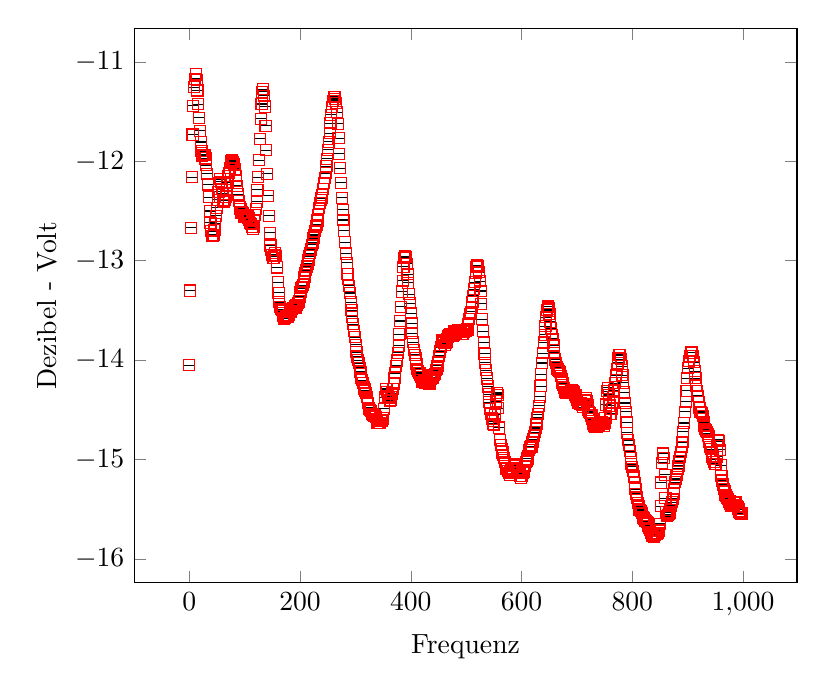
\begin{tikzpicture}
		\pgfplotsset{width=10cm,legend style={font=\footnotesize}}
		\begin{axis}[xlabel={Frequenz},ylabel={Dezibel - Volt},legend cell align=left,legend pos=north west]
		\addplot+[only marks,color=red,mark=square,error bars/.cd,x dir=both,x explicit,y dir=both,y explicit,error bar style={color=black}] table[x=X,y=Y,x error=xerror,y error=yerror,row sep=\\]{
			X	Y	xerror	yerror	\\
			0.0	-14.050505	0	0	\\
			1.464844	-13.299937	0	0	\\
			2.929687	-12.667614	0	0	\\
			4.394531	-12.158621	0	0	\\
			5.859375	-11.730596	0	0	\\
			7.324219	-11.439429	0	0	\\
			8.789062	-11.255181	0	0	\\
			10.253906	-11.167565	0	0	\\
			11.71875	-11.125702	0	0	\\
			13.183594	-11.185375	0	0	\\
			14.648437	-11.286533	0	0	\\
			16.113281	-11.424848	0	0	\\
			17.578125	-11.562135	0	0	\\
			19.042969	-11.692611	0	0	\\
			20.507812	-11.805825	0	0	\\
			21.972656	-11.897202	0	0	\\
			23.4375	-11.942884	0	0	\\
			24.902344	-11.933558	0	0	\\
			26.367187	-11.933213	0	0	\\
			27.832031	-11.935169	0	0	\\
			29.296875	-11.970685	0	0	\\
			30.761719	-12.03641	0	0	\\
			32.226562	-12.12475	0	0	\\
			33.691406	-12.233002	0	0	\\
			35.15625	-12.362489	0	0	\\
			36.621094	-12.499766	0	0	\\
			38.085937	-12.616361	0	0	\\
			39.550781	-12.703513	0	0	\\
			41.015625	-12.752819	0	0	\\
			42.480469	-12.748154	0	0	\\
			43.945312	-12.73773	0	0	\\
			45.410156	-12.692056	0	0	\\
			46.875	-12.627846	0	0	\\
			48.339844	-12.546045	0	0	\\
			49.804687	-12.465853	0	0	\\
			51.269531	-12.387216	0	0	\\
			52.734375	-12.307693	0	0	\\
			54.199219	-12.223723	0	0	\\
			55.664062	-12.177003	0	0	\\
			57.128906	-12.203774	0	0	\\
			58.59375	-12.277561	0	0	\\
			60.058594	-12.328262	0	0	\\
			61.523437	-12.396147	0	0	\\
			62.988281	-12.410666	0	0	\\
			64.453125	-12.386562	0	0	\\
			65.917969	-12.354418	0	0	\\
			67.382812	-12.29202	0	0	\\
			68.847656	-12.212931	0	0	\\
			70.3125	-12.149613	0	0	\\
			71.777344	-12.118436	0	0	\\
			73.242187	-12.069843	0	0	\\
			74.707031	-12.020032	0	0	\\
			76.171875	-11.994096	0	0	\\
			77.636719	-11.985539	0	0	\\
			79.101562	-12.006559	0	0	\\
			80.566406	-12.031732	0	0	\\
			82.03125	-12.072989	0	0	\\
			83.496094	-12.143531	0	0	\\
			84.960937	-12.194586	0	0	\\
			86.425781	-12.247041	0	0	\\
			87.890625	-12.333256	0	0	\\
			89.355469	-12.397348	0	0	\\
			90.820312	-12.458001	0	0	\\
			92.285156	-12.479244	0	0	\\
			93.75	-12.519968	0	0	\\
			95.214844	-12.511867	0	0	\\
			96.679687	-12.51593	0	0	\\
			98.144531	-12.543087	0	0	\\
			99.609375	-12.555055	0	0	\\
			101.074219	-12.546762	0	0	\\
			102.539062	-12.546863	0	0	\\
			104.003906	-12.555903	0	0	\\
			105.46875	-12.550551	0	0	\\
			106.933594	-12.566872	0	0	\\
			108.398437	-12.584899	0	0	\\
			109.863281	-12.619747	0	0	\\
			111.328125	-12.628088	0	0	\\
			112.792969	-12.660742	0	0	\\
			114.257812	-12.683404	0	0	\\
			115.722656	-12.657223	0	0	\\
			117.1875	-12.598691	0	0	\\
			118.652344	-12.537689	0	0	\\
			120.117187	-12.48002	0	0	\\
			121.582031	-12.406897	0	0	\\
			123.046875	-12.28631	0	0	\\
			124.511719	-12.161429	0	0	\\
			125.976562	-11.990362	0	0	\\
			127.441406	-11.771233	0	0	\\
			128.90625	-11.571997	0	0	\\
			130.371094	-11.422843	0	0	\\
			131.835937	-11.299549	0	0	\\
			133.300781	-11.275164	0	0	\\
			134.765625	-11.341789	0	0	\\
			136.230469	-11.44871	0	0	\\
			137.695312	-11.641409	0	0	\\
			139.160156	-11.889627	0	0	\\
			140.625	-12.125895	0	0	\\
			142.089844	-12.345694	0	0	\\
			143.554687	-12.548676	0	0	\\
			145.019531	-12.719376	0	0	\\
			146.484375	-12.846957	0	0	\\
			147.949219	-12.888508	0	0	\\
			149.414062	-12.94263	0	0	\\
			150.878906	-12.973352	0	0	\\
			152.34375	-12.972911	0	0	\\
			153.808594	-12.946934	0	0	\\
			155.273437	-12.918748	0	0	\\
			156.738281	-12.955085	0	0	\\
			158.203125	-13.067271	0	0	\\
			159.667969	-13.216498	0	0	\\
			161.132812	-13.32257	0	0	\\
			162.597656	-13.415944	0	0	\\
			164.0625	-13.466877	0	0	\\
			165.527344	-13.488856	0	0	\\
			166.992187	-13.493699	0	0	\\
			168.457031	-13.509316	0	0	\\
			169.921875	-13.556178	0	0	\\
			171.386719	-13.580522	0	0	\\
			172.851562	-13.573926	0	0	\\
			174.316406	-13.561218	0	0	\\
			175.78125	-13.558925	0	0	\\
			177.246094	-13.560324	0	0	\\
			178.710937	-13.56292	0	0	\\
			180.175781	-13.545437	0	0	\\
			181.640625	-13.517522	0	0	\\
			183.105469	-13.509958	0	0	\\
			184.570312	-13.486111	0	0	\\
			186.035156	-13.4824	0	0	\\
			187.5	-13.479368	0	0	\\
			188.964844	-13.472779	0	0	\\
			190.429687	-13.460141	0	0	\\
			191.894531	-13.469727	0	0	\\
			193.359375	-13.44579	0	0	\\
			194.824219	-13.444059	0	0	\\
			196.289062	-13.42621	0	0	\\
			197.753906	-13.409402	0	0	\\
			199.21875	-13.362461	0	0	\\
			200.683594	-13.314831	0	0	\\
			202.148437	-13.274704	0	0	\\
			203.613281	-13.263993	0	0	\\
			205.078125	-13.246126	0	0	\\
			206.542969	-13.209223	0	0	\\
			208.007812	-13.162423	0	0	\\
			209.472656	-13.119143	0	0	\\
			210.9375	-13.09283	0	0	\\
			212.402344	-13.058518	0	0	\\
			213.867187	-13.032045	0	0	\\
			215.332031	-12.995536	0	0	\\
			216.796875	-12.953788	0	0	\\
			218.261719	-12.923639	0	0	\\
			219.726562	-12.886046	0	0	\\
			221.191406	-12.838865	0	0	\\
			222.65625	-12.819288	0	0	\\
			224.121094	-12.773106	0	0	\\
			225.585937	-12.740998	0	0	\\
			227.050781	-12.696878	0	0	\\
			228.515625	-12.655263	0	0	\\
			229.980469	-12.636984	0	0	\\
			231.445312	-12.59561	0	0	\\
			232.910156	-12.536112	0	0	\\
			234.375	-12.473359	0	0	\\
			235.839844	-12.415836	0	0	\\
			237.304687	-12.390182	0	0	\\
			238.769531	-12.369233	0	0	\\
			240.234375	-12.336422	0	0	\\
			241.699219	-12.280003	0	0	\\
			243.164062	-12.221002	0	0	\\
			244.628906	-12.170596	0	0	\\
			246.09375	-12.119882	0	0	\\
			247.558594	-12.050278	0	0	\\
			249.023437	-11.97433	0	0	\\
			250.488281	-11.884071	0	0	\\
			251.953125	-11.801957	0	0	\\
			253.417969	-11.715909	0	0	\\
			254.882812	-11.615192	0	0	\\
			256.347656	-11.531232	0	0	\\
			257.8125	-11.450738	0	0	\\
			259.277344	-11.391323	0	0	\\
			260.742187	-11.35611	0	0	\\
			262.207031	-11.349498	0	0	\\
			263.671875	-11.372311	0	0	\\
			265.136719	-11.411729	0	0	\\
			266.601562	-11.506046	0	0	\\
			268.066406	-11.621456	0	0	\\
			269.53125	-11.767096	0	0	\\
			270.996094	-11.922912	0	0	\\
			272.460937	-12.070072	0	0	\\
			273.925781	-12.213813	0	0	\\
			275.390625	-12.365535	0	0	\\
			276.855469	-12.488526	0	0	\\
			278.320312	-12.589865	0	0	\\
			279.785156	-12.696111	0	0	\\
			281.25	-12.813684	0	0	\\
			282.714844	-12.927304	0	0	\\
			284.179687	-13.021632	0	0	\\
			285.644531	-13.131017	0	0	\\
			287.109375	-13.186065	0	0	\\
			288.574219	-13.250932	0	0	\\
			290.039062	-13.323876	0	0	\\
			291.503906	-13.419504	0	0	\\
			292.96875	-13.499429	0	0	\\
			294.433594	-13.562529	0	0	\\
			295.898437	-13.637796	0	0	\\
			297.363281	-13.707288	0	0	\\
			298.828125	-13.769209	0	0	\\
			300.292969	-13.846533	0	0	\\
			301.757812	-13.917909	0	0	\\
			303.222656	-13.965913	0	0	\\
			304.6875	-14.002488	0	0	\\
			306.152344	-14.031927	0	0	\\
			307.617187	-14.0776	0	0	\\
			309.082031	-14.119358	0	0	\\
			310.546875	-14.177657	0	0	\\
			312.011719	-14.202594	0	0	\\
			313.476562	-14.233382	0	0	\\
			314.941406	-14.275084	0	0	\\
			316.40625	-14.286332	0	0	\\
			317.871094	-14.305431	0	0	\\
			319.335937	-14.329957	0	0	\\
			320.800781	-14.372081	0	0	\\
			322.265625	-14.431703	0	0	\\
			323.730469	-14.479415	0	0	\\
			325.195312	-14.488866	0	0	\\
			326.660156	-14.504204	0	0	\\
			328.125	-14.513373	0	0	\\
			329.589844	-14.545465	0	0	\\
			331.054687	-14.551137	0	0	\\
			332.519531	-14.554262	0	0	\\
			333.984375	-14.560821	0	0	\\
			335.449219	-14.557158	0	0	\\
			336.914062	-14.57582	0	0	\\
			338.378906	-14.606307	0	0	\\
			339.84375	-14.633411	0	0	\\
			341.308594	-14.628931	0	0	\\
			342.773437	-14.635881	0	0	\\
			344.238281	-14.62858	0	0	\\
			345.703125	-14.605059	0	0	\\
			347.167969	-14.611538	0	0	\\
			348.632812	-14.608422	0	0	\\
			350.097656	-14.586239	0	0	\\
			351.5625	-14.488962	0	0	\\
			353.027344	-14.371365	0	0	\\
			354.492187	-14.290249	0	0	\\
			355.957031	-14.290229	0	0	\\
			357.421875	-14.320078	0	0	\\
			358.886719	-14.358496	0	0	\\
			360.351562	-14.382988	0	0	\\
			361.816406	-14.406957	0	0	\\
			363.28125	-14.398909	0	0	\\
			364.746094	-14.367863	0	0	\\
			366.210937	-14.335484	0	0	\\
			367.675781	-14.29155	0	0	\\
			369.140625	-14.235703	0	0	\\
			370.605469	-14.179809	0	0	\\
			372.070312	-14.129939	0	0	\\
			373.535156	-14.057932	0	0	\\
			375.0	-14.004341	0	0	\\
			376.464844	-13.924224	0	0	\\
			377.929687	-13.855575	0	0	\\
			379.394531	-13.738273	0	0	\\
			380.859375	-13.605998	0	0	\\
			382.324219	-13.464516	0	0	\\
			383.789062	-13.309787	0	0	\\
			385.253906	-13.200063	0	0	\\
			386.71875	-13.060897	0	0	\\
			388.183594	-12.97622	0	0	\\
			389.648437	-12.956916	0	0	\\
			391.113281	-12.965539	0	0	\\
			392.578125	-13.030482	0	0	\\
			394.042969	-13.1343	0	0	\\
			395.507812	-13.22321	0	0	\\
			396.972656	-13.335253	0	0	\\
			398.4375	-13.428647	0	0	\\
			399.902344	-13.529227	0	0	\\
			401.367187	-13.62814	0	0	\\
			402.832031	-13.727482	0	0	\\
			404.296875	-13.819466	0	0	\\
			405.761719	-13.896711	0	0	\\
			407.226562	-13.944845	0	0	\\
			408.691406	-13.982526	0	0	\\
			410.15625	-14.041802	0	0	\\
			411.621094	-14.085652	0	0	\\
			413.085937	-14.111029	0	0	\\
			414.550781	-14.128493	0	0	\\
			416.015625	-14.133768	0	0	\\
			417.480469	-14.151043	0	0	\\
			418.945312	-14.170855	0	0	\\
			420.410156	-14.216436	0	0	\\
			421.875	-14.217036	0	0	\\
			423.339844	-14.210892	0	0	\\
			424.804687	-14.21458	0	0	\\
			426.269531	-14.225149	0	0	\\
			427.734375	-14.225299	0	0	\\
			429.199219	-14.223484	0	0	\\
			430.664062	-14.23328	0	0	\\
			432.128906	-14.242844	0	0	\\
			433.59375	-14.238656	0	0	\\
			435.058594	-14.195949	0	0	\\
			436.523437	-14.18551	0	0	\\
			437.988281	-14.178383	0	0	\\
			439.453125	-14.177931	0	0	\\
			440.917969	-14.15285	0	0	\\
			442.382812	-14.147003	0	0	\\
			443.847656	-14.135528	0	0	\\
			445.3125	-14.102925	0	0	\\
			446.777344	-14.083479	0	0	\\
			448.242187	-14.057502	0	0	\\
			449.707031	-14.018939	0	0	\\
			451.171875	-13.958109	0	0	\\
			452.636719	-13.912992	0	0	\\
			454.101562	-13.87162	0	0	\\
			455.566406	-13.80972	0	0	\\
			457.03125	-13.802168	0	0	\\
			458.496094	-13.814805	0	0	\\
			459.960937	-13.828085	0	0	\\
			461.425781	-13.843606	0	0	\\
			462.890625	-13.825697	0	0	\\
			464.355469	-13.815212	0	0	\\
			465.820312	-13.78755	0	0	\\
			467.285156	-13.76159	0	0	\\
			468.75	-13.750413	0	0	\\
			470.214844	-13.749508	0	0	\\
			471.679687	-13.739326	0	0	\\
			473.144531	-13.73774	0	0	\\
			474.609375	-13.741617	0	0	\\
			476.074219	-13.756798	0	0	\\
			477.539062	-13.743379	0	0	\\
			479.003906	-13.711689	0	0	\\
			480.46875	-13.715047	0	0	\\
			481.933594	-13.730951	0	0	\\
			483.398437	-13.720465	0	0	\\
			484.863281	-13.696815	0	0	\\
			486.328125	-13.714307	0	0	\\
			487.792969	-13.712178	0	0	\\
			489.257812	-13.715804	0	0	\\
			490.722656	-13.717373	0	0	\\
			492.1875	-13.733816	0	0	\\
			493.652344	-13.7371	0	0	\\
			495.117187	-13.716919	0	0	\\
			496.582031	-13.704679	0	0	\\
			498.046875	-13.707767	0	0	\\
			499.511719	-13.706872	0	0	\\
			500.976562	-13.685887	0	0	\\
			502.441406	-13.691197	0	0	\\
			503.90625	-13.64209	0	0	\\
			505.371094	-13.58796	0	0	\\
			506.835937	-13.535002	0	0	\\
			508.300781	-13.513402	0	0	\\
			509.765625	-13.478852	0	0	\\
			511.230469	-13.412173	0	0	\\
			512.695312	-13.350785	0	0	\\
			514.160156	-13.286017	0	0	\\
			515.625	-13.216078	0	0	\\
			517.089844	-13.119241	0	0	\\
			518.554687	-13.065301	0	0	\\
			520.019531	-13.047169	0	0	\\
			521.484375	-13.05185	0	0	\\
			522.949219	-13.114488	0	0	\\
			524.414062	-13.204968	0	0	\\
			525.878906	-13.304042	0	0	\\
			527.34375	-13.4332	0	0	\\
			528.808594	-13.587725	0	0	\\
			530.273437	-13.707911	0	0	\\
			531.738281	-13.822526	0	0	\\
			533.203125	-13.936431	0	0	\\
			534.667969	-14.026417	0	0	\\
			536.132812	-14.102635	0	0	\\
			537.597656	-14.184221	0	0	\\
			539.0625	-14.264295	0	0	\\
			540.527344	-14.341433	0	0	\\
			541.992187	-14.422495	0	0	\\
			543.457031	-14.48791	0	0	\\
			544.921875	-14.536511	0	0	\\
			546.386719	-14.587397	0	0	\\
			547.851562	-14.612427	0	0	\\
			549.316406	-14.641665	0	0	\\
			550.78125	-14.647993	0	0	\\
			552.246094	-14.546999	0	0	\\
			553.710937	-14.415276	0	0	\\
			555.175781	-14.330225	0	0	\\
			556.640625	-14.350996	0	0	\\
			558.105469	-14.482412	0	0	\\
			559.570312	-14.677802	0	0	\\
			561.035156	-14.800089	0	0	\\
			562.5	-14.85551	0	0	\\
			563.964844	-14.894614	0	0	\\
			565.429687	-14.928676	0	0	\\
			566.894531	-14.952805	0	0	\\
			568.359375	-14.98422	0	0	\\
			569.824219	-15.028166	0	0	\\
			571.289062	-15.083012	0	0	\\
			572.753906	-15.090926	0	0	\\
			574.21875	-15.094026	0	0	\\
			575.683594	-15.114998	0	0	\\
			577.148437	-15.136628	0	0	\\
			578.613281	-15.15258	0	0	\\
			580.078125	-15.122533	0	0	\\
			581.542969	-15.107289	0	0	\\
			583.007812	-15.094602	0	0	\\
			584.472656	-15.082529	0	0	\\
			585.9375	-15.059935	0	0	\\
			587.402344	-15.058453	0	0	\\
			588.867187	-15.046029	0	0	\\
			590.332031	-15.06678	0	0	\\
			591.796875	-15.099119	0	0	\\
			593.261719	-15.135108	0	0	\\
			594.726562	-15.128433	0	0	\\
			596.191406	-15.137806	0	0	\\
			597.65625	-15.166473	0	0	\\
			599.121094	-15.180882	0	0	\\
			600.585937	-15.163743	0	0	\\
			602.050781	-15.133186	0	0	\\
			603.515625	-15.125595	0	0	\\
			604.980469	-15.115409	0	0	\\
			606.445312	-15.067269	0	0	\\
			607.910156	-15.023027	0	0	\\
			609.375	-15.009752	0	0	\\
			610.839844	-14.989937	0	0	\\
			612.304687	-14.967128	0	0	\\
			613.769531	-14.905996	0	0	\\
			615.234375	-14.878592	0	0	\\
			616.699219	-14.866289	0	0	\\
			618.164062	-14.868215	0	0	\\
			619.628906	-14.822102	0	0	\\
			621.09375	-14.793859	0	0	\\
			622.558594	-14.766284	0	0	\\
			624.023437	-14.725277	0	0	\\
			625.488281	-14.682154	0	0	\\
			626.953125	-14.640055	0	0	\\
			628.417969	-14.581117	0	0	\\
			629.882812	-14.545271	0	0	\\
			631.347656	-14.459573	0	0	\\
			632.8125	-14.366694	0	0	\\
			634.277344	-14.263101	0	0	\\
			635.742187	-14.142677	0	0	\\
			637.207031	-14.028242	0	0	\\
			638.671875	-13.931155	0	0	\\
			640.136719	-13.822631	0	0	\\
			641.601562	-13.745261	0	0	\\
			643.066406	-13.658316	0	0	\\
			644.53125	-13.569186	0	0	\\
			645.996094	-13.495608	0	0	\\
			647.460937	-13.46108	0	0	\\
			648.925781	-13.480555	0	0	\\
			650.390625	-13.538272	0	0	\\
			651.855469	-13.613028	0	0	\\
			653.320312	-13.681032	0	0	\\
			654.785156	-13.744338	0	0	\\
			656.25	-13.784262	0	0	\\
			657.714844	-13.851768	0	0	\\
			659.179687	-13.924064	0	0	\\
			660.644531	-13.993007	0	0	\\
			662.109375	-14.025634	0	0	\\
			663.574219	-14.069885	0	0	\\
			665.039062	-14.087395	0	0	\\
			666.503906	-14.10298	0	0	\\
			667.96875	-14.1068	0	0	\\
			669.433594	-14.122748	0	0	\\
			670.898437	-14.162633	0	0	\\
			672.363281	-14.192739	0	0	\\
			673.828125	-14.230496	0	0	\\
			675.292969	-14.247783	0	0	\\
			676.757812	-14.283354	0	0	\\
			678.222656	-14.316979	0	0	\\
			679.6875	-14.33117	0	0	\\
			681.152344	-14.326027	0	0	\\
			682.617187	-14.322572	0	0	\\
			684.082031	-14.322422	0	0	\\
			685.546875	-14.318143	0	0	\\
			687.011719	-14.32596	0	0	\\
			688.476562	-14.322964	0	0	\\
			689.941406	-14.308299	0	0	\\
			691.40625	-14.298386	0	0	\\
			692.871094	-14.307418	0	0	\\
			694.335937	-14.324684	0	0	\\
			695.800781	-14.351422	0	0	\\
			697.265625	-14.352408	0	0	\\
			698.730469	-14.36568	0	0	\\
			700.195312	-14.404201	0	0	\\
			701.660156	-14.430898	0	0	\\
			703.125	-14.427039	0	0	\\
			704.589844	-14.434381	0	0	\\
			706.054687	-14.435618	0	0	\\
			707.519531	-14.432911	0	0	\\
			708.984375	-14.446435	0	0	\\
			710.449219	-14.475005	0	0	\\
			711.914062	-14.452262	0	0	\\
			713.378906	-14.437378	0	0	\\
			714.84375	-14.404899	0	0	\\
			716.308594	-14.385541	0	0	\\
			717.773437	-14.415438	0	0	\\
			719.238281	-14.454149	0	0	\\
			720.703125	-14.497398	0	0	\\
			722.167969	-14.520317	0	0	\\
			723.632812	-14.529866	0	0	\\
			725.097656	-14.557658	0	0	\\
			726.5625	-14.555079	0	0	\\
			728.027344	-14.596049	0	0	\\
			729.492187	-14.638483	0	0	\\
			730.957031	-14.66205	0	0	\\
			732.421875	-14.675452	0	0	\\
			733.886719	-14.675422	0	0	\\
			735.351562	-14.672214	0	0	\\
			736.816406	-14.656058	0	0	\\
			738.28125	-14.651118	0	0	\\
			739.746094	-14.649747	0	0	\\
			741.210937	-14.636523	0	0	\\
			742.675781	-14.636155	0	0	\\
			744.140625	-14.6218	0	0	\\
			745.605469	-14.625461	0	0	\\
			747.070312	-14.643622	0	0	\\
			748.535156	-14.657819	0	0	\\
			750.0	-14.631515	0	0	\\
			751.464844	-14.582607	0	0	\\
			752.929687	-14.446605	0	0	\\
			754.394531	-14.312882	0	0	\\
			755.859375	-14.276123	0	0	\\
			757.324219	-14.350377	0	0	\\
			758.789062	-14.456408	0	0	\\
			760.253906	-14.541881	0	0	\\
			761.71875	-14.537256	0	0	\\
			763.183594	-14.488729	0	0	\\
			764.648437	-14.427315	0	0	\\
			766.113281	-14.37244	0	0	\\
			767.578125	-14.305331	0	0	\\
			769.042969	-14.232469	0	0	\\
			770.507812	-14.155074	0	0	\\
			771.972656	-14.091079	0	0	\\
			773.4375	-14.027252	0	0	\\
			774.902344	-13.975445	0	0	\\
			776.367187	-13.949346	0	0	\\
			777.832031	-13.947627	0	0	\\
			779.296875	-13.991495	0	0	\\
			780.761719	-14.061561	0	0	\\
			782.226562	-14.150668	0	0	\\
			783.691406	-14.228971	0	0	\\
			785.15625	-14.324549	0	0	\\
			786.621094	-14.430608	0	0	\\
			788.085937	-14.51929	0	0	\\
			789.550781	-14.623041	0	0	\\
			791.015625	-14.730229	0	0	\\
			792.480469	-14.805449	0	0	\\
			793.945312	-14.852743	0	0	\\
			795.410156	-14.914466	0	0	\\
			796.875	-14.986443	0	0	\\
			798.339844	-15.047592	0	0	\\
			799.804687	-15.071631	0	0	\\
			801.269531	-15.114165	0	0	\\
			802.734375	-15.170488	0	0	\\
			804.199219	-15.239781	0	0	\\
			805.664062	-15.295695	0	0	\\
			807.128906	-15.346834	0	0	\\
			808.59375	-15.382291	0	0	\\
			810.058594	-15.438962	0	0	\\
			811.523437	-15.472461	0	0	\\
			812.988281	-15.505756	0	0	\\
			814.453125	-15.51089	0	0	\\
			815.917969	-15.516134	0	0	\\
			817.382812	-15.538309	0	0	\\
			818.847656	-15.577786	0	0	\\
			820.3125	-15.590476	0	0	\\
			821.777344	-15.592755	0	0	\\
			823.242187	-15.613741	0	0	\\
			824.707031	-15.614099	0	0	\\
			826.171875	-15.625513	0	0	\\
			827.636719	-15.638591	0	0	\\
			829.101562	-15.667989	0	0	\\
			830.566406	-15.689446	0	0	\\
			832.03125	-15.711343	0	0	\\
			833.496094	-15.735803	0	0	\\
			834.960937	-15.748217	0	0	\\
			836.425781	-15.766733	0	0	\\
			837.890625	-15.762721	0	0	\\
			839.355469	-15.775128	0	0	\\
			840.820312	-15.754851	0	0	\\
			842.285156	-15.745726	0	0	\\
			843.75	-15.746132	0	0	\\
			845.214844	-15.740792	0	0	\\
			846.679687	-15.737162	0	0	\\
			848.144531	-15.713806	0	0	\\
			849.609375	-15.648701	0	0	\\
			851.074219	-15.469149	0	0	\\
			852.539062	-15.231399	0	0	\\
			854.003906	-15.031341	0	0	\\
			855.46875	-14.939818	0	0	\\
			856.933594	-14.982826	0	0	\\
			858.398437	-15.151275	0	0	\\
			859.863281	-15.387465	0	0	\\
			861.328125	-15.525493	0	0	\\
			862.792969	-15.567574	0	0	\\
			864.257812	-15.55716	0	0	\\
			865.722656	-15.548389	0	0	\\
			867.1875	-15.531781	0	0	\\
			868.652344	-15.507071	0	0	\\
			870.117187	-15.465653	0	0	\\
			871.582031	-15.428138	0	0	\\
			873.046875	-15.396552	0	0	\\
			874.511719	-15.348787	0	0	\\
			875.976562	-15.293764	0	0	\\
			877.441406	-15.22911	0	0	\\
			878.90625	-15.195975	0	0	\\
			880.371094	-15.153742	0	0	\\
			881.835937	-15.092107	0	0	\\
			883.300781	-15.062193	0	0	\\
			884.765625	-15.016929	0	0	\\
			886.230469	-14.972279	0	0	\\
			887.695312	-14.925672	0	0	\\
			889.160156	-14.876122	0	0	\\
			890.625	-14.823821	0	0	\\
			892.089844	-14.721841	0	0	\\
			893.554687	-14.631986	0	0	\\
			895.019531	-14.519774	0	0	\\
			896.484375	-14.418282	0	0	\\
			897.949219	-14.308576	0	0	\\
			899.414062	-14.181744	0	0	\\
			900.878906	-14.079504	0	0	\\
			902.34375	-14.009096	0	0	\\
			903.808594	-13.95814	0	0	\\
			905.273437	-13.9262	0	0	\\
			906.738281	-13.923177	0	0	\\
			908.203125	-13.923957	0	0	\\
			909.667969	-13.960398	0	0	\\
			911.132812	-14.021155	0	0	\\
			912.597656	-14.111932	0	0	\\
			914.0625	-14.180354	0	0	\\
			915.527344	-14.255244	0	0	\\
			916.992187	-14.309459	0	0	\\
			918.457031	-14.359127	0	0	\\
			919.921875	-14.424297	0	0	\\
			921.386719	-14.477953	0	0	\\
			922.851562	-14.520959	0	0	\\
			924.316406	-14.525141	0	0	\\
			925.78125	-14.531666	0	0	\\
			927.246094	-14.565809	0	0	\\
			928.710937	-14.625074	0	0	\\
			930.175781	-14.658041	0	0	\\
			931.640625	-14.69385	0	0	\\
			933.105469	-14.708211	0	0	\\
			934.570312	-14.722134	0	0	\\
			936.035156	-14.739455	0	0	\\
			937.5	-14.760567	0	0	\\
			938.964844	-14.818323	0	0	\\
			940.429687	-14.870238	0	0	\\
			941.894531	-14.895099	0	0	\\
			943.359375	-14.929479	0	0	\\
			944.824219	-14.969275	0	0	\\
			946.289062	-14.994583	0	0	\\
			947.753906	-15.021683	0	0	\\
			949.21875	-15.047419	0	0	\\
			950.683594	-15.04475	0	0	\\
			952.148437	-14.970457	0	0	\\
			953.613281	-14.866085	0	0	\\
			955.078125	-14.799097	0	0	\\
			956.542969	-14.815702	0	0	\\
			958.007812	-14.901837	0	0	\\
			959.472656	-15.057832	0	0	\\
			960.9375	-15.162472	0	0	\\
			962.402344	-15.21057	0	0	\\
			963.867187	-15.250887	0	0	\\
			965.332031	-15.297959	0	0	\\
			966.796875	-15.320597	0	0	\\
			968.261719	-15.355816	0	0	\\
			969.726562	-15.367667	0	0	\\
			971.191406	-15.382371	0	0	\\
			972.65625	-15.395509	0	0	\\
			974.121094	-15.422016	0	0	\\
			975.585937	-15.420453	0	0	\\
			977.050781	-15.441803	0	0	\\
			978.515625	-15.462805	0	0	\\
			979.980469	-15.46989	0	0	\\
			981.445312	-15.467675	0	0	\\
			982.910156	-15.459868	0	0	\\
			984.375	-15.437176	0	0	\\
			985.839844	-15.428645	0	0	\\
			987.304687	-15.429379	0	0	\\
			988.769531	-15.463354	0	0	\\
			990.234375	-15.476478	0	0	\\
			991.699219	-15.500575	0	0	\\
			993.164062	-15.521667	0	0	\\
			994.628906	-15.539474	0	0	\\
			996.09375	-15.54427	0	0	\\
			997.558594	-15.541833	0	0	\\
		};		% \addlegendentry{Messpunkte Datensatz 0}
		\end{axis}
		\end{tikzpicture}
	\caption{$T=0\si\degree$}
	\label{fig:Umgebungsmessung}
\end{figure}

    \subsection*{Background noise}
        Before we start with the analysis of the data, we have to consider the background noise. We measured the background noise for the first measurement and obtained the following results:
        \input{Sektionen/AuswertungsergebnisseFreiheit/Graphen/ÜbungsMessung.tex}
        These we will then consider when choosing the peaks in the following analysis to not mistake them for false ones. 

    \subsection*{Analysis of first measure}
        We start analysing from high to low temperature. We will present the graphs and tables each. 
        
        \subsubsection*{73 degrees}
            \begin{figure}[H]
	\centering
	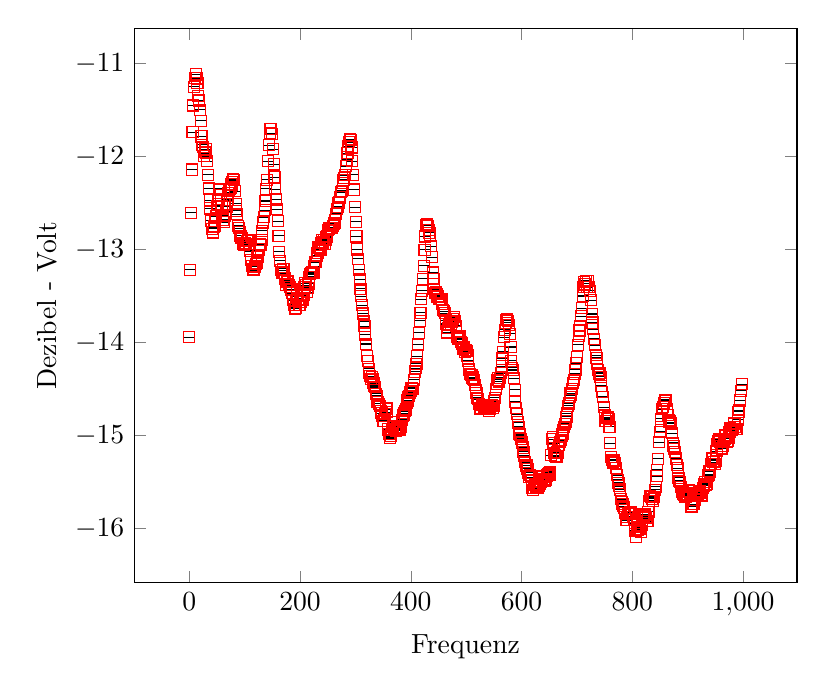
\begin{tikzpicture}
		\pgfplotsset{width=10cm,legend style={font=\footnotesize}}
		\begin{axis}[xlabel={Frequenz},ylabel={Dezibel - Volt},legend cell align=left,legend pos=north west]
		\addplot+[only marks,color=red,mark=square,error bars/.cd,x dir=both,x explicit,y dir=both,y explicit,error bar style={color=black}] table[x=X,y=Y,x error=xerror,y error=yerror,row sep=\\]{
			X	Y	xerror	yerror	\\
			0.0	-13.944471	0	0	\\
			1.464844	-13.218628	0	0	\\
			2.929687	-12.60769	0	0	\\
			4.394531	-12.141175	0	0	\\
			5.859375	-11.741029	0	0	\\
			7.324219	-11.452051	0	0	\\
			8.789062	-11.249477	0	0	\\
			10.253906	-11.158565	0	0	\\
			11.71875	-11.117902	0	0	\\
			13.183594	-11.161134	0	0	\\
			14.648437	-11.211065	0	0	\\
			16.113281	-11.346855	0	0	\\
			17.578125	-11.398137	0	0	\\
			19.042969	-11.4989	0	0	\\
			20.507812	-11.616372	0	0	\\
			21.972656	-11.784753	0	0	\\
			23.4375	-11.873724	0	0	\\
			24.902344	-11.901582	0	0	\\
			26.367187	-11.996939	0	0	\\
			27.832031	-11.952896	0	0	\\
			29.296875	-11.923208	0	0	\\
			30.761719	-11.966716	0	0	\\
			32.226562	-12.051753	0	0	\\
			33.691406	-12.198508	0	0	\\
			35.15625	-12.344775	0	0	\\
			36.621094	-12.473229	0	0	\\
			38.085937	-12.559498	0	0	\\
			39.550781	-12.692169	0	0	\\
			41.015625	-12.779751	0	0	\\
			42.480469	-12.817506	0	0	\\
			43.945312	-12.759275	0	0	\\
			45.410156	-12.750344	0	0	\\
			46.875	-12.696855	0	0	\\
			48.339844	-12.645603	0	0	\\
			49.804687	-12.538719	0	0	\\
			51.269531	-12.515609	0	0	\\
			52.734375	-12.454646	0	0	\\
			54.199219	-12.359051	0	0	\\
			55.664062	-12.346734	0	0	\\
			57.128906	-12.415251	0	0	\\
			58.59375	-12.530745	0	0	\\
			60.058594	-12.635092	0	0	\\
			61.523437	-12.678688	0	0	\\
			62.988281	-12.704896	0	0	\\
			64.453125	-12.641397	0	0	\\
			65.917969	-12.587232	0	0	\\
			67.382812	-12.53973	0	0	\\
			68.847656	-12.468172	0	0	\\
			70.3125	-12.390512	0	0	\\
			71.777344	-12.365978	0	0	\\
			73.242187	-12.353352	0	0	\\
			74.707031	-12.334407	0	0	\\
			76.171875	-12.301089	0	0	\\
			77.636719	-12.273698	0	0	\\
			79.101562	-12.240015	0	0	\\
			80.566406	-12.253447	0	0	\\
			82.03125	-12.375394	0	0	\\
			83.496094	-12.508262	0	0	\\
			84.960937	-12.583697	0	0	\\
			86.425781	-12.619764	0	0	\\
			87.890625	-12.745579	0	0	\\
			89.355469	-12.773291	0	0	\\
			90.820312	-12.811458	0	0	\\
			92.285156	-12.8547	0	0	\\
			93.75	-12.880704	0	0	\\
			95.214844	-12.881597	0	0	\\
			96.679687	-12.943458	0	0	\\
			98.144531	-12.954904	0	0	\\
			99.609375	-12.944888	0	0	\\
			101.074219	-12.930625	0	0	\\
			102.539062	-12.944276	0	0	\\
			104.003906	-12.913877	0	0	\\
			105.46875	-12.896136	0	0	\\
			106.933594	-12.904053	0	0	\\
			108.398437	-12.941211	0	0	\\
			109.863281	-13.017003	0	0	\\
			111.328125	-13.118068	0	0	\\
			112.792969	-13.181165	0	0	\\
			114.257812	-13.210408	0	0	\\
			115.722656	-13.222059	0	0	\\
			117.1875	-13.206618	0	0	\\
			118.652344	-13.18745	0	0	\\
			120.117187	-13.160107	0	0	\\
			121.582031	-13.141237	0	0	\\
			123.046875	-13.085509	0	0	\\
			124.511719	-13.056335	0	0	\\
			125.976562	-13.000671	0	0	\\
			127.441406	-12.942684	0	0	\\
			128.90625	-12.951481	0	0	\\
			130.371094	-12.894858	0	0	\\
			131.835937	-12.798687	0	0	\\
			133.300781	-12.709976	0	0	\\
			134.765625	-12.652854	0	0	\\
			136.230469	-12.579898	0	0	\\
			137.695312	-12.478897	0	0	\\
			139.160156	-12.349247	0	0	\\
			140.625	-12.251687	0	0	\\
			142.089844	-12.050942	0	0	\\
			143.554687	-11.878436	0	0	\\
			145.019531	-11.749454	0	0	\\
			146.484375	-11.701087	0	0	\\
			147.949219	-11.700373	0	0	\\
			149.414062	-11.762814	0	0	\\
			150.878906	-11.920982	0	0	\\
			152.34375	-12.086076	0	0	\\
			153.808594	-12.224746	0	0	\\
			155.273437	-12.354517	0	0	\\
			156.738281	-12.462491	0	0	\\
			158.203125	-12.569243	0	0	\\
			159.667969	-12.697632	0	0	\\
			161.132812	-12.85369	0	0	\\
			162.597656	-13.025272	0	0	\\
			164.0625	-13.122604	0	0	\\
			165.527344	-13.224956	0	0	\\
			166.992187	-13.253829	0	0	\\
			168.457031	-13.25797	0	0	\\
			169.921875	-13.207248	0	0	\\
			171.386719	-13.248703	0	0	\\
			172.851562	-13.312195	0	0	\\
			174.316406	-13.377979	0	0	\\
			175.78125	-13.336645	0	0	\\
			177.246094	-13.35217	0	0	\\
			178.710937	-13.34573	0	0	\\
			180.175781	-13.384513	0	0	\\
			181.640625	-13.408233	0	0	\\
			183.105469	-13.435046	0	0	\\
			184.570312	-13.427732	0	0	\\
			186.035156	-13.472448	0	0	\\
			187.5	-13.545692	0	0	\\
			188.964844	-13.596029	0	0	\\
			190.429687	-13.639801	0	0	\\
			191.894531	-13.628171	0	0	\\
			193.359375	-13.557249	0	0	\\
			194.824219	-13.501319	0	0	\\
			196.289062	-13.529682	0	0	\\
			197.753906	-13.59435	0	0	\\
			199.21875	-13.596339	0	0	\\
			200.683594	-13.563706	0	0	\\
			202.148437	-13.538814	0	0	\\
			203.613281	-13.536267	0	0	\\
			205.078125	-13.544189	0	0	\\
			206.542969	-13.494117	0	0	\\
			208.007812	-13.405475	0	0	\\
			209.472656	-13.363182	0	0	\\
			210.9375	-13.385856	0	0	\\
			212.402344	-13.46236	0	0	\\
			213.867187	-13.416484	0	0	\\
			215.332031	-13.368327	0	0	\\
			216.796875	-13.296043	0	0	\\
			218.261719	-13.263946	0	0	\\
			219.726562	-13.257138	0	0	\\
			221.191406	-13.240819	0	0	\\
			222.65625	-13.249893	0	0	\\
			224.121094	-13.256779	0	0	\\
			225.585937	-13.180697	0	0	\\
			227.050781	-13.137939	0	0	\\
			228.515625	-13.13289	0	0	\\
			229.980469	-13.068613	0	0	\\
			231.445312	-13.03647	0	0	\\
			232.910156	-12.97851	0	0	\\
			234.375	-12.987958	0	0	\\
			235.839844	-12.995954	0	0	\\
			237.304687	-13.003028	0	0	\\
			238.769531	-12.932255	0	0	\\
			240.234375	-12.90124	0	0	\\
			241.699219	-12.925771	0	0	\\
			243.164062	-12.895974	0	0	\\
			244.628906	-12.937637	0	0	\\
			246.09375	-12.899736	0	0	\\
			247.558594	-12.870586	0	0	\\
			249.023437	-12.858518	0	0	\\
			250.488281	-12.787242	0	0	\\
			251.953125	-12.774146	0	0	\\
			253.417969	-12.766766	0	0	\\
			254.882812	-12.766072	0	0	\\
			256.347656	-12.766291	0	0	\\
			257.8125	-12.766131	0	0	\\
			259.277344	-12.745827	0	0	\\
			260.742187	-12.723559	0	0	\\
			262.207031	-12.718322	0	0	\\
			263.671875	-12.68439	0	0	\\
			265.136719	-12.616666	0	0	\\
			266.601562	-12.561203	0	0	\\
			268.066406	-12.539476	0	0	\\
			269.53125	-12.499734	0	0	\\
			270.996094	-12.488675	0	0	\\
			272.460937	-12.441403	0	0	\\
			273.925781	-12.384141	0	0	\\
			275.390625	-12.372125	0	0	\\
			276.855469	-12.286503	0	0	\\
			278.320312	-12.24962	0	0	\\
			279.785156	-12.230826	0	0	\\
			281.25	-12.202706	0	0	\\
			282.714844	-12.102675	0	0	\\
			284.179687	-12.037275	0	0	\\
			285.644531	-11.963993	0	0	\\
			287.109375	-11.890521	0	0	\\
			288.574219	-11.844678	0	0	\\
			290.039062	-11.814098	0	0	\\
			291.503906	-11.823036	0	0	\\
			292.96875	-11.902914	0	0	\\
			294.433594	-12.050198	0	0	\\
			295.898437	-12.197382	0	0	\\
			297.363281	-12.356081	0	0	\\
			298.828125	-12.546665	0	0	\\
			300.292969	-12.701117	0	0	\\
			301.757812	-12.860263	0	0	\\
			303.222656	-13.000226	0	0	\\
			304.6875	-13.100011	0	0	\\
			306.152344	-13.218447	0	0	\\
			307.617187	-13.323501	0	0	\\
			309.082031	-13.422369	0	0	\\
			310.546875	-13.501773	0	0	\\
			312.011719	-13.600167	0	0	\\
			313.476562	-13.68956	0	0	\\
			314.941406	-13.776085	0	0	\\
			316.40625	-13.825046	0	0	\\
			317.871094	-13.914549	0	0	\\
			319.335937	-14.017291	0	0	\\
			320.800781	-14.143981	0	0	\\
			322.265625	-14.201067	0	0	\\
			323.730469	-14.283797	0	0	\\
			325.195312	-14.333463	0	0	\\
			326.660156	-14.362655	0	0	\\
			328.125	-14.39513	0	0	\\
			329.589844	-14.37248	0	0	\\
			331.054687	-14.393551	0	0	\\
			332.519531	-14.438617	0	0	\\
			333.984375	-14.46365	0	0	\\
			335.449219	-14.480571	0	0	\\
			336.914062	-14.55467	0	0	\\
			338.378906	-14.57541	0	0	\\
			339.84375	-14.637146	0	0	\\
			341.308594	-14.637175	0	0	\\
			342.773437	-14.66142	0	0	\\
			344.238281	-14.683445	0	0	\\
			345.703125	-14.739505	0	0	\\
			347.167969	-14.762295	0	0	\\
			348.632812	-14.795823	0	0	\\
			350.097656	-14.849707	0	0	\\
			351.5625	-14.841125	0	0	\\
			353.027344	-14.767082	0	0	\\
			354.492187	-14.717885	0	0	\\
			355.957031	-14.706983	0	0	\\
			357.421875	-14.753139	0	0	\\
			358.886719	-14.93686	0	0	\\
			360.351562	-14.987807	0	0	\\
			361.816406	-15.028744	0	0	\\
			363.28125	-15.00958	0	0	\\
			364.746094	-14.986256	0	0	\\
			366.210937	-14.938313	0	0	\\
			367.675781	-14.900853	0	0	\\
			369.140625	-14.859244	0	0	\\
			370.605469	-14.915338	0	0	\\
			372.070312	-14.93831	0	0	\\
			373.535156	-14.951109	0	0	\\
			375.0	-14.919264	0	0	\\
			376.464844	-14.925843	0	0	\\
			377.929687	-14.927466	0	0	\\
			379.394531	-14.944752	0	0	\\
			380.859375	-14.917676	0	0	\\
			382.324219	-14.911064	0	0	\\
			383.789062	-14.833353	0	0	\\
			385.253906	-14.794458	0	0	\\
			386.71875	-14.777003	0	0	\\
			388.183594	-14.762655	0	0	\\
			389.648437	-14.741056	0	0	\\
			391.113281	-14.722468	0	0	\\
			392.578125	-14.656089	0	0	\\
			394.042969	-14.624511	0	0	\\
			395.507812	-14.584727	0	0	\\
			396.972656	-14.573375	0	0	\\
			398.4375	-14.538434	0	0	\\
			399.902344	-14.52219	0	0	\\
			401.367187	-14.490736	0	0	\\
			402.832031	-14.497974	0	0	\\
			404.296875	-14.497345	0	0	\\
			405.761719	-14.403138	0	0	\\
			407.226562	-14.314085	0	0	\\
			408.691406	-14.276795	0	0	\\
			410.15625	-14.230695	0	0	\\
			411.621094	-14.149248	0	0	\\
			413.085937	-14.022943	0	0	\\
			414.550781	-13.896144	0	0	\\
			416.015625	-13.765987	0	0	\\
			417.480469	-13.683342	0	0	\\
			418.945312	-13.53428	0	0	\\
			420.410156	-13.444636	0	0	\\
			421.875	-13.316637	0	0	\\
			423.339844	-13.175632	0	0	\\
			424.804687	-13.003827	0	0	\\
			426.269531	-12.861132	0	0	\\
			427.734375	-12.736735	0	0	\\
			429.199219	-12.727476	0	0	\\
			430.664062	-12.747351	0	0	\\
			432.128906	-12.791325	0	0	\\
			433.59375	-12.820658	0	0	\\
			435.058594	-12.854948	0	0	\\
			436.523437	-12.96389	0	0	\\
			437.988281	-13.084389	0	0	\\
			439.453125	-13.248909	0	0	\\
			440.917969	-13.315121	0	0	\\
			442.382812	-13.426718	0	0	\\
			443.847656	-13.471992	0	0	\\
			445.3125	-13.457287	0	0	\\
			446.777344	-13.476225	0	0	\\
			448.242187	-13.509281	0	0	\\
			449.707031	-13.501175	0	0	\\
			451.171875	-13.537795	0	0	\\
			452.636719	-13.537614	0	0	\\
			454.101562	-13.537497	0	0	\\
			455.566406	-13.529049	0	0	\\
			457.03125	-13.591064	0	0	\\
			458.496094	-13.648225	0	0	\\
			459.960937	-13.665812	0	0	\\
			461.425781	-13.687221	0	0	\\
			462.890625	-13.761158	0	0	\\
			464.355469	-13.802799	0	0	\\
			465.820312	-13.893707	0	0	\\
			467.285156	-13.842652	0	0	\\
			468.75	-13.814306	0	0	\\
			470.214844	-13.778938	0	0	\\
			471.679687	-13.781903	0	0	\\
			473.144531	-13.802782	0	0	\\
			474.609375	-13.782766	0	0	\\
			476.074219	-13.750391	0	0	\\
			477.539062	-13.729134	0	0	\\
			479.003906	-13.769806	0	0	\\
			480.46875	-13.767564	0	0	\\
			481.933594	-13.822662	0	0	\\
			483.398437	-13.941027	0	0	\\
			484.863281	-13.967739	0	0	\\
			486.328125	-13.95642	0	0	\\
			487.792969	-13.93721	0	0	\\
			489.257812	-13.944364	0	0	\\
			490.722656	-13.992701	0	0	\\
			492.1875	-14.011239	0	0	\\
			493.652344	-14.074031	0	0	\\
			495.117187	-14.058389	0	0	\\
			496.582031	-14.05231	0	0	\\
			498.046875	-14.102584	0	0	\\
			499.511719	-14.08063	0	0	\\
			500.976562	-14.095954	0	0	\\
			502.441406	-14.141648	0	0	\\
			503.90625	-14.199574	0	0	\\
			505.371094	-14.292513	0	0	\\
			506.835937	-14.342627	0	0	\\
			508.300781	-14.346556	0	0	\\
			509.765625	-14.3543	0	0	\\
			511.230469	-14.378662	0	0	\\
			512.695312	-14.39205	0	0	\\
			514.160156	-14.401136	0	0	\\
			515.625	-14.458383	0	0	\\
			517.089844	-14.5145	0	0	\\
			518.554687	-14.545935	0	0	\\
			520.019531	-14.59685	0	0	\\
			521.484375	-14.611129	0	0	\\
			522.949219	-14.666533	0	0	\\
			524.414062	-14.71703	0	0	\\
			525.878906	-14.702909	0	0	\\
			527.34375	-14.70853	0	0	\\
			528.808594	-14.670805	0	0	\\
			530.273437	-14.672267	0	0	\\
			531.738281	-14.69602	0	0	\\
			533.203125	-14.679773	0	0	\\
			534.667969	-14.687149	0	0	\\
			536.132812	-14.688838	0	0	\\
			537.597656	-14.684397	0	0	\\
			539.0625	-14.699907	0	0	\\
			540.527344	-14.735897	0	0	\\
			541.992187	-14.716112	0	0	\\
			543.457031	-14.710752	0	0	\\
			544.921875	-14.687977	0	0	\\
			546.386719	-14.670953	0	0	\\
			547.851562	-14.704329	0	0	\\
			549.316406	-14.684968	0	0	\\
			550.78125	-14.630869	0	0	\\
			552.246094	-14.597656	0	0	\\
			553.710937	-14.505954	0	0	\\
			555.175781	-14.444022	0	0	\\
			556.640625	-14.402177	0	0	\\
			558.105469	-14.385234	0	0	\\
			559.570312	-14.420059	0	0	\\
			561.035156	-14.379676	0	0	\\
			562.5	-14.333834	0	0	\\
			563.964844	-14.255669	0	0	\\
			565.429687	-14.173801	0	0	\\
			566.894531	-14.102304	0	0	\\
			568.359375	-13.943775	0	0	\\
			569.824219	-13.865548	0	0	\\
			571.289062	-13.788322	0	0	\\
			572.753906	-13.758116	0	0	\\
			574.21875	-13.754412	0	0	\\
			575.683594	-13.767614	0	0	\\
			577.148437	-13.810125	0	0	\\
			578.613281	-13.907848	0	0	\\
			580.078125	-14.04967	0	0	\\
			581.542969	-14.199365	0	0	\\
			583.007812	-14.271518	0	0	\\
			584.472656	-14.296674	0	0	\\
			585.9375	-14.386687	0	0	\\
			587.402344	-14.510152	0	0	\\
			588.867187	-14.640319	0	0	\\
			590.332031	-14.70888	0	0	\\
			591.796875	-14.774532	0	0	\\
			593.261719	-14.861688	0	0	\\
			594.726562	-14.910425	0	0	\\
			596.191406	-14.98195	0	0	\\
			597.65625	-14.996569	0	0	\\
			599.121094	-15.037669	0	0	\\
			600.585937	-15.077797	0	0	\\
			602.050781	-15.131254	0	0	\\
			603.515625	-15.176684	0	0	\\
			604.980469	-15.217383	0	0	\\
			606.445312	-15.289591	0	0	\\
			607.910156	-15.323754	0	0	\\
			609.375	-15.32428	0	0	\\
			610.839844	-15.360672	0	0	\\
			612.304687	-15.403515	0	0	\\
			613.769531	-15.450175	0	0	\\
			615.234375	-15.423166	0	0	\\
			616.699219	-15.433057	0	0	\\
			618.164062	-15.486894	0	0	\\
			619.628906	-15.570838	0	0	\\
			621.09375	-15.584244	0	0	\\
			622.558594	-15.563721	0	0	\\
			624.023437	-15.531904	0	0	\\
			625.488281	-15.528757	0	0	\\
			626.953125	-15.550579	0	0	\\
			628.417969	-15.557608	0	0	\\
			629.882812	-15.561039	0	0	\\
			631.347656	-15.548705	0	0	\\
			632.8125	-15.519282	0	0	\\
			634.277344	-15.501333	0	0	\\
			635.742187	-15.473194	0	0	\\
			637.207031	-15.469528	0	0	\\
			638.671875	-15.443163	0	0	\\
			640.136719	-15.471451	0	0	\\
			641.601562	-15.486887	0	0	\\
			643.066406	-15.481984	0	0	\\
			644.53125	-15.46822	0	0	\\
			645.996094	-15.432798	0	0	\\
			647.460937	-15.421824	0	0	\\
			648.925781	-15.403651	0	0	\\
			650.390625	-15.428911	0	0	\\
			651.855469	-15.392459	0	0	\\
			653.320312	-15.214365	0	0	\\
			654.785156	-15.040799	0	0	\\
			656.25	-15.019704	0	0	\\
			657.714844	-15.082795	0	0	\\
			659.179687	-15.193071	0	0	\\
			660.644531	-15.217559	0	0	\\
			662.109375	-15.23239	0	0	\\
			663.574219	-15.23089	0	0	\\
			665.039062	-15.184462	0	0	\\
			666.503906	-15.132194	0	0	\\
			667.96875	-15.107932	0	0	\\
			669.433594	-15.070447	0	0	\\
			670.898437	-15.050131	0	0	\\
			672.363281	-15.010623	0	0	\\
			673.828125	-14.989426	0	0	\\
			675.292969	-14.946257	0	0	\\
			676.757812	-14.907106	0	0	\\
			678.222656	-14.874861	0	0	\\
			679.6875	-14.850349	0	0	\\
			681.152344	-14.798424	0	0	\\
			682.617187	-14.763837	0	0	\\
			684.082031	-14.682101	0	0	\\
			685.546875	-14.656988	0	0	\\
			687.011719	-14.59062	0	0	\\
			688.476562	-14.546267	0	0	\\
			689.941406	-14.566493	0	0	\\
			691.40625	-14.501333	0	0	\\
			692.871094	-14.441339	0	0	\\
			694.335937	-14.403616	0	0	\\
			695.800781	-14.33902	0	0	\\
			697.265625	-14.295951	0	0	\\
			698.730469	-14.223634	0	0	\\
			700.195312	-14.158067	0	0	\\
			701.660156	-14.027315	0	0	\\
			703.125	-13.932481	0	0	\\
			704.589844	-13.872199	0	0	\\
			706.054687	-13.822815	0	0	\\
			707.519531	-13.718135	0	0	\\
			708.984375	-13.63279	0	0	\\
			710.449219	-13.501634	0	0	\\
			711.914062	-13.402344	0	0	\\
			713.378906	-13.348868	0	0	\\
			714.84375	-13.37144	0	0	\\
			716.308594	-13.336207	0	0	\\
			717.773437	-13.405103	0	0	\\
			719.238281	-13.344171	0	0	\\
			720.703125	-13.342639	0	0	\\
			722.167969	-13.403023	0	0	\\
			723.632812	-13.444673	0	0	\\
			725.097656	-13.547066	0	0	\\
			726.5625	-13.695242	0	0	\\
			728.027344	-13.786537	0	0	\\
			729.492187	-13.857549	0	0	\\
			730.957031	-13.963897	0	0	\\
			732.421875	-14.03139	0	0	\\
			733.886719	-14.140159	0	0	\\
			735.351562	-14.16651	0	0	\\
			736.816406	-14.230729	0	0	\\
			738.28125	-14.296164	0	0	\\
			739.746094	-14.334641	0	0	\\
			741.210937	-14.329275	0	0	\\
			742.675781	-14.370539	0	0	\\
			744.140625	-14.467219	0	0	\\
			745.605469	-14.531827	0	0	\\
			747.070312	-14.583495	0	0	\\
			748.535156	-14.697794	0	0	\\
			750.0	-14.786569	0	0	\\
			751.464844	-14.849499	0	0	\\
			752.929687	-14.848566	0	0	\\
			754.394531	-14.816746	0	0	\\
			755.859375	-14.807675	0	0	\\
			757.324219	-14.823869	0	0	\\
			758.789062	-14.908406	0	0	\\
			760.253906	-15.085575	0	0	\\
			761.71875	-15.234924	0	0	\\
			763.183594	-15.261746	0	0	\\
			764.648437	-15.292001	0	0	\\
			766.113281	-15.273074	0	0	\\
			767.578125	-15.268497	0	0	\\
			769.042969	-15.294751	0	0	\\
			770.507812	-15.352574	0	0	\\
			771.972656	-15.427966	0	0	\\
			773.4375	-15.478346	0	0	\\
			774.902344	-15.509839	0	0	\\
			776.367187	-15.54485	0	0	\\
			777.832031	-15.583446	0	0	\\
			779.296875	-15.687774	0	0	\\
			780.761719	-15.717089	0	0	\\
			782.226562	-15.736434	0	0	\\
			783.691406	-15.764384	0	0	\\
			785.15625	-15.776802	0	0	\\
			786.621094	-15.837355	0	0	\\
			788.085937	-15.905927	0	0	\\
			789.550781	-15.9109	0	0	\\
			791.015625	-15.875569	0	0	\\
			792.480469	-15.848251	0	0	\\
			793.945312	-15.847396	0	0	\\
			795.410156	-15.823541	0	0	\\
			796.875	-15.829923	0	0	\\
			798.339844	-15.82127	0	0	\\
			799.804687	-15.847274	0	0	\\
			801.269531	-15.876796	0	0	\\
			802.734375	-15.905272	0	0	\\
			804.199219	-15.94542	0	0	\\
			805.664062	-16.023803	0	0	\\
			807.128906	-16.089433	0	0	\\
			808.59375	-16.016709	0	0	\\
			810.058594	-16.013508	0	0	\\
			811.523437	-15.990251	0	0	\\
			812.988281	-16.007226	0	0	\\
			814.453125	-15.986158	0	0	\\
			815.917969	-16.034829	0	0	\\
			817.382812	-15.968	0	0	\\
			818.847656	-15.892651	0	0	\\
			820.3125	-15.870638	0	0	\\
			821.777344	-15.848883	0	0	\\
			823.242187	-15.852079	0	0	\\
			824.707031	-15.883786	0	0	\\
			826.171875	-15.918997	0	0	\\
			827.636719	-15.923488	0	0	\\
			829.101562	-15.821191	0	0	\\
			830.566406	-15.70647	0	0	\\
			832.03125	-15.652331	0	0	\\
			833.496094	-15.661485	0	0	\\
			834.960937	-15.665487	0	0	\\
			836.425781	-15.682887	0	0	\\
			837.890625	-15.709029	0	0	\\
			839.355469	-15.660995	0	0	\\
			840.820312	-15.585292	0	0	\\
			842.285156	-15.553211	0	0	\\
			843.75	-15.437059	0	0	\\
			845.214844	-15.36853	0	0	\\
			846.679687	-15.25177	0	0	\\
			848.144531	-15.072892	0	0	\\
			849.609375	-14.96344	0	0	\\
			851.074219	-14.906902	0	0	\\
			852.539062	-14.822843	0	0	\\
			854.003906	-14.720787	0	0	\\
			855.46875	-14.694269	0	0	\\
			856.933594	-14.654292	0	0	\\
			858.398437	-14.629808	0	0	\\
			859.863281	-14.616036	0	0	\\
			861.328125	-14.632258	0	0	\\
			862.792969	-14.720911	0	0	\\
			864.257812	-14.779922	0	0	\\
			865.722656	-14.835606	0	0	\\
			867.1875	-14.857485	0	0	\\
			868.652344	-14.842156	0	0	\\
			870.117187	-14.872574	0	0	\\
			871.582031	-14.976067	0	0	\\
			873.046875	-15.078117	0	0	\\
			874.511719	-15.116492	0	0	\\
			875.976562	-15.145783	0	0	\\
			877.441406	-15.183484	0	0	\\
			878.90625	-15.249494	0	0	\\
			880.371094	-15.315832	0	0	\\
			881.835937	-15.352098	0	0	\\
			883.300781	-15.45737	0	0	\\
			884.765625	-15.489204	0	0	\\
			886.230469	-15.499059	0	0	\\
			887.695312	-15.558827	0	0	\\
			889.160156	-15.604945	0	0	\\
			890.625	-15.600385	0	0	\\
			892.089844	-15.630406	0	0	\\
			893.554687	-15.64477	0	0	\\
			895.019531	-15.657829	0	0	\\
			896.484375	-15.661049	0	0	\\
			897.949219	-15.638733	0	0	\\
			899.414062	-15.642555	0	0	\\
			900.878906	-15.634869	0	0	\\
			902.34375	-15.593759	0	0	\\
			903.808594	-15.625502	0	0	\\
			905.273437	-15.741353	0	0	\\
			906.738281	-15.768944	0	0	\\
			908.203125	-15.763954	0	0	\\
			909.667969	-15.741365	0	0	\\
			911.132812	-15.740473	0	0	\\
			912.597656	-15.694883	0	0	\\
			914.0625	-15.641633	0	0	\\
			915.527344	-15.632309	0	0	\\
			916.992187	-15.619794	0	0	\\
			918.457031	-15.627323	0	0	\\
			919.921875	-15.613578	0	0	\\
			921.386719	-15.616595	0	0	\\
			922.851562	-15.601726	0	0	\\
			924.316406	-15.641107	0	0	\\
			925.78125	-15.654087	0	0	\\
			927.246094	-15.563979	0	0	\\
			928.710937	-15.540728	0	0	\\
			930.175781	-15.522229	0	0	\\
			931.640625	-15.504444	0	0	\\
			933.105469	-15.528893	0	0	\\
			934.570312	-15.523504	0	0	\\
			936.035156	-15.435019	0	0	\\
			937.5	-15.425332	0	0	\\
			938.964844	-15.382462	0	0	\\
			940.429687	-15.38911	0	0	\\
			941.894531	-15.312656	0	0	\\
			943.359375	-15.244778	0	0	\\
			944.824219	-15.255819	0	0	\\
			946.289062	-15.287437	0	0	\\
			947.753906	-15.289783	0	0	\\
			949.21875	-15.309993	0	0	\\
			950.683594	-15.273668	0	0	\\
			952.148437	-15.170406	0	0	\\
			953.613281	-15.090493	0	0	\\
			955.078125	-15.056735	0	0	\\
			956.542969	-15.045634	0	0	\\
			958.007812	-15.072196	0	0	\\
			959.472656	-15.111009	0	0	\\
			960.9375	-15.138774	0	0	\\
			962.402344	-15.143305	0	0	\\
			963.867187	-15.115052	0	0	\\
			965.332031	-15.069476	0	0	\\
			966.796875	-15.036253	0	0	\\
			968.261719	-15.000561	0	0	\\
			969.726562	-15.012249	0	0	\\
			971.191406	-15.06547	0	0	\\
			972.65625	-15.06399	0	0	\\
			974.121094	-15.022663	0	0	\\
			975.585937	-14.959842	0	0	\\
			977.050781	-14.925161	0	0	\\
			978.515625	-14.936986	0	0	\\
			979.980469	-14.94617	0	0	\\
			981.445312	-14.931677	0	0	\\
			982.910156	-14.877084	0	0	\\
			984.375	-14.869712	0	0	\\
			985.839844	-14.913588	0	0	\\
			987.304687	-14.934401	0	0	\\
			988.769531	-14.930792	0	0	\\
			990.234375	-14.833539	0	0	\\
			991.699219	-14.747825	0	0	\\
			993.164062	-14.730986	0	0	\\
			994.628906	-14.624443	0	0	\\
			996.09375	-14.521525	0	0	\\
			997.558594	-14.450173	0	0	\\
		};		% \addlegendentry{Messpunkte Datensatz 0}
		\end{axis}
		\end{tikzpicture}
	\caption{$T=73\si\degree$}
	\label{fig:Umgebungsmessung}
\end{figure}
            \begin{figure}[H]
	\centering
	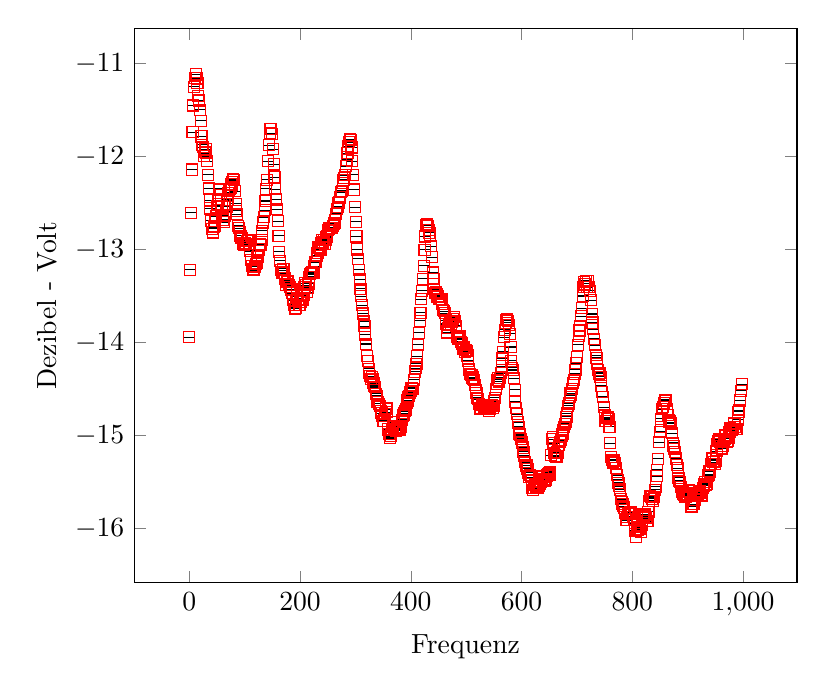
\begin{tikzpicture}
		\pgfplotsset{width=10cm,legend style={font=\footnotesize}}
		\begin{axis}[xlabel={Frequenz},ylabel={Dezibel - Volt},legend cell align=left,legend pos=north west]
		\addplot+[only marks,color=red,mark=square,error bars/.cd,x dir=both,x explicit,y dir=both,y explicit,error bar style={color=black}] table[x=X,y=Y,x error=xerror,y error=yerror,row sep=\\]{
			X	Y	xerror	yerror	\\
			0.0	-13.944471	0	0	\\
			1.464844	-13.218628	0	0	\\
			2.929687	-12.60769	0	0	\\
			4.394531	-12.141175	0	0	\\
			5.859375	-11.741029	0	0	\\
			7.324219	-11.452051	0	0	\\
			8.789062	-11.249477	0	0	\\
			10.253906	-11.158565	0	0	\\
			11.71875	-11.117902	0	0	\\
			13.183594	-11.161134	0	0	\\
			14.648437	-11.211065	0	0	\\
			16.113281	-11.346855	0	0	\\
			17.578125	-11.398137	0	0	\\
			19.042969	-11.4989	0	0	\\
			20.507812	-11.616372	0	0	\\
			21.972656	-11.784753	0	0	\\
			23.4375	-11.873724	0	0	\\
			24.902344	-11.901582	0	0	\\
			26.367187	-11.996939	0	0	\\
			27.832031	-11.952896	0	0	\\
			29.296875	-11.923208	0	0	\\
			30.761719	-11.966716	0	0	\\
			32.226562	-12.051753	0	0	\\
			33.691406	-12.198508	0	0	\\
			35.15625	-12.344775	0	0	\\
			36.621094	-12.473229	0	0	\\
			38.085937	-12.559498	0	0	\\
			39.550781	-12.692169	0	0	\\
			41.015625	-12.779751	0	0	\\
			42.480469	-12.817506	0	0	\\
			43.945312	-12.759275	0	0	\\
			45.410156	-12.750344	0	0	\\
			46.875	-12.696855	0	0	\\
			48.339844	-12.645603	0	0	\\
			49.804687	-12.538719	0	0	\\
			51.269531	-12.515609	0	0	\\
			52.734375	-12.454646	0	0	\\
			54.199219	-12.359051	0	0	\\
			55.664062	-12.346734	0	0	\\
			57.128906	-12.415251	0	0	\\
			58.59375	-12.530745	0	0	\\
			60.058594	-12.635092	0	0	\\
			61.523437	-12.678688	0	0	\\
			62.988281	-12.704896	0	0	\\
			64.453125	-12.641397	0	0	\\
			65.917969	-12.587232	0	0	\\
			67.382812	-12.53973	0	0	\\
			68.847656	-12.468172	0	0	\\
			70.3125	-12.390512	0	0	\\
			71.777344	-12.365978	0	0	\\
			73.242187	-12.353352	0	0	\\
			74.707031	-12.334407	0	0	\\
			76.171875	-12.301089	0	0	\\
			77.636719	-12.273698	0	0	\\
			79.101562	-12.240015	0	0	\\
			80.566406	-12.253447	0	0	\\
			82.03125	-12.375394	0	0	\\
			83.496094	-12.508262	0	0	\\
			84.960937	-12.583697	0	0	\\
			86.425781	-12.619764	0	0	\\
			87.890625	-12.745579	0	0	\\
			89.355469	-12.773291	0	0	\\
			90.820312	-12.811458	0	0	\\
			92.285156	-12.8547	0	0	\\
			93.75	-12.880704	0	0	\\
			95.214844	-12.881597	0	0	\\
			96.679687	-12.943458	0	0	\\
			98.144531	-12.954904	0	0	\\
			99.609375	-12.944888	0	0	\\
			101.074219	-12.930625	0	0	\\
			102.539062	-12.944276	0	0	\\
			104.003906	-12.913877	0	0	\\
			105.46875	-12.896136	0	0	\\
			106.933594	-12.904053	0	0	\\
			108.398437	-12.941211	0	0	\\
			109.863281	-13.017003	0	0	\\
			111.328125	-13.118068	0	0	\\
			112.792969	-13.181165	0	0	\\
			114.257812	-13.210408	0	0	\\
			115.722656	-13.222059	0	0	\\
			117.1875	-13.206618	0	0	\\
			118.652344	-13.18745	0	0	\\
			120.117187	-13.160107	0	0	\\
			121.582031	-13.141237	0	0	\\
			123.046875	-13.085509	0	0	\\
			124.511719	-13.056335	0	0	\\
			125.976562	-13.000671	0	0	\\
			127.441406	-12.942684	0	0	\\
			128.90625	-12.951481	0	0	\\
			130.371094	-12.894858	0	0	\\
			131.835937	-12.798687	0	0	\\
			133.300781	-12.709976	0	0	\\
			134.765625	-12.652854	0	0	\\
			136.230469	-12.579898	0	0	\\
			137.695312	-12.478897	0	0	\\
			139.160156	-12.349247	0	0	\\
			140.625	-12.251687	0	0	\\
			142.089844	-12.050942	0	0	\\
			143.554687	-11.878436	0	0	\\
			145.019531	-11.749454	0	0	\\
			146.484375	-11.701087	0	0	\\
			147.949219	-11.700373	0	0	\\
			149.414062	-11.762814	0	0	\\
			150.878906	-11.920982	0	0	\\
			152.34375	-12.086076	0	0	\\
			153.808594	-12.224746	0	0	\\
			155.273437	-12.354517	0	0	\\
			156.738281	-12.462491	0	0	\\
			158.203125	-12.569243	0	0	\\
			159.667969	-12.697632	0	0	\\
			161.132812	-12.85369	0	0	\\
			162.597656	-13.025272	0	0	\\
			164.0625	-13.122604	0	0	\\
			165.527344	-13.224956	0	0	\\
			166.992187	-13.253829	0	0	\\
			168.457031	-13.25797	0	0	\\
			169.921875	-13.207248	0	0	\\
			171.386719	-13.248703	0	0	\\
			172.851562	-13.312195	0	0	\\
			174.316406	-13.377979	0	0	\\
			175.78125	-13.336645	0	0	\\
			177.246094	-13.35217	0	0	\\
			178.710937	-13.34573	0	0	\\
			180.175781	-13.384513	0	0	\\
			181.640625	-13.408233	0	0	\\
			183.105469	-13.435046	0	0	\\
			184.570312	-13.427732	0	0	\\
			186.035156	-13.472448	0	0	\\
			187.5	-13.545692	0	0	\\
			188.964844	-13.596029	0	0	\\
			190.429687	-13.639801	0	0	\\
			191.894531	-13.628171	0	0	\\
			193.359375	-13.557249	0	0	\\
			194.824219	-13.501319	0	0	\\
			196.289062	-13.529682	0	0	\\
			197.753906	-13.59435	0	0	\\
			199.21875	-13.596339	0	0	\\
			200.683594	-13.563706	0	0	\\
			202.148437	-13.538814	0	0	\\
			203.613281	-13.536267	0	0	\\
			205.078125	-13.544189	0	0	\\
			206.542969	-13.494117	0	0	\\
			208.007812	-13.405475	0	0	\\
			209.472656	-13.363182	0	0	\\
			210.9375	-13.385856	0	0	\\
			212.402344	-13.46236	0	0	\\
			213.867187	-13.416484	0	0	\\
			215.332031	-13.368327	0	0	\\
			216.796875	-13.296043	0	0	\\
			218.261719	-13.263946	0	0	\\
			219.726562	-13.257138	0	0	\\
			221.191406	-13.240819	0	0	\\
			222.65625	-13.249893	0	0	\\
			224.121094	-13.256779	0	0	\\
			225.585937	-13.180697	0	0	\\
			227.050781	-13.137939	0	0	\\
			228.515625	-13.13289	0	0	\\
			229.980469	-13.068613	0	0	\\
			231.445312	-13.03647	0	0	\\
			232.910156	-12.97851	0	0	\\
			234.375	-12.987958	0	0	\\
			235.839844	-12.995954	0	0	\\
			237.304687	-13.003028	0	0	\\
			238.769531	-12.932255	0	0	\\
			240.234375	-12.90124	0	0	\\
			241.699219	-12.925771	0	0	\\
			243.164062	-12.895974	0	0	\\
			244.628906	-12.937637	0	0	\\
			246.09375	-12.899736	0	0	\\
			247.558594	-12.870586	0	0	\\
			249.023437	-12.858518	0	0	\\
			250.488281	-12.787242	0	0	\\
			251.953125	-12.774146	0	0	\\
			253.417969	-12.766766	0	0	\\
			254.882812	-12.766072	0	0	\\
			256.347656	-12.766291	0	0	\\
			257.8125	-12.766131	0	0	\\
			259.277344	-12.745827	0	0	\\
			260.742187	-12.723559	0	0	\\
			262.207031	-12.718322	0	0	\\
			263.671875	-12.68439	0	0	\\
			265.136719	-12.616666	0	0	\\
			266.601562	-12.561203	0	0	\\
			268.066406	-12.539476	0	0	\\
			269.53125	-12.499734	0	0	\\
			270.996094	-12.488675	0	0	\\
			272.460937	-12.441403	0	0	\\
			273.925781	-12.384141	0	0	\\
			275.390625	-12.372125	0	0	\\
			276.855469	-12.286503	0	0	\\
			278.320312	-12.24962	0	0	\\
			279.785156	-12.230826	0	0	\\
			281.25	-12.202706	0	0	\\
			282.714844	-12.102675	0	0	\\
			284.179687	-12.037275	0	0	\\
			285.644531	-11.963993	0	0	\\
			287.109375	-11.890521	0	0	\\
			288.574219	-11.844678	0	0	\\
			290.039062	-11.814098	0	0	\\
			291.503906	-11.823036	0	0	\\
			292.96875	-11.902914	0	0	\\
			294.433594	-12.050198	0	0	\\
			295.898437	-12.197382	0	0	\\
			297.363281	-12.356081	0	0	\\
			298.828125	-12.546665	0	0	\\
			300.292969	-12.701117	0	0	\\
			301.757812	-12.860263	0	0	\\
			303.222656	-13.000226	0	0	\\
			304.6875	-13.100011	0	0	\\
			306.152344	-13.218447	0	0	\\
			307.617187	-13.323501	0	0	\\
			309.082031	-13.422369	0	0	\\
			310.546875	-13.501773	0	0	\\
			312.011719	-13.600167	0	0	\\
			313.476562	-13.68956	0	0	\\
			314.941406	-13.776085	0	0	\\
			316.40625	-13.825046	0	0	\\
			317.871094	-13.914549	0	0	\\
			319.335937	-14.017291	0	0	\\
			320.800781	-14.143981	0	0	\\
			322.265625	-14.201067	0	0	\\
			323.730469	-14.283797	0	0	\\
			325.195312	-14.333463	0	0	\\
			326.660156	-14.362655	0	0	\\
			328.125	-14.39513	0	0	\\
			329.589844	-14.37248	0	0	\\
			331.054687	-14.393551	0	0	\\
			332.519531	-14.438617	0	0	\\
			333.984375	-14.46365	0	0	\\
			335.449219	-14.480571	0	0	\\
			336.914062	-14.55467	0	0	\\
			338.378906	-14.57541	0	0	\\
			339.84375	-14.637146	0	0	\\
			341.308594	-14.637175	0	0	\\
			342.773437	-14.66142	0	0	\\
			344.238281	-14.683445	0	0	\\
			345.703125	-14.739505	0	0	\\
			347.167969	-14.762295	0	0	\\
			348.632812	-14.795823	0	0	\\
			350.097656	-14.849707	0	0	\\
			351.5625	-14.841125	0	0	\\
			353.027344	-14.767082	0	0	\\
			354.492187	-14.717885	0	0	\\
			355.957031	-14.706983	0	0	\\
			357.421875	-14.753139	0	0	\\
			358.886719	-14.93686	0	0	\\
			360.351562	-14.987807	0	0	\\
			361.816406	-15.028744	0	0	\\
			363.28125	-15.00958	0	0	\\
			364.746094	-14.986256	0	0	\\
			366.210937	-14.938313	0	0	\\
			367.675781	-14.900853	0	0	\\
			369.140625	-14.859244	0	0	\\
			370.605469	-14.915338	0	0	\\
			372.070312	-14.93831	0	0	\\
			373.535156	-14.951109	0	0	\\
			375.0	-14.919264	0	0	\\
			376.464844	-14.925843	0	0	\\
			377.929687	-14.927466	0	0	\\
			379.394531	-14.944752	0	0	\\
			380.859375	-14.917676	0	0	\\
			382.324219	-14.911064	0	0	\\
			383.789062	-14.833353	0	0	\\
			385.253906	-14.794458	0	0	\\
			386.71875	-14.777003	0	0	\\
			388.183594	-14.762655	0	0	\\
			389.648437	-14.741056	0	0	\\
			391.113281	-14.722468	0	0	\\
			392.578125	-14.656089	0	0	\\
			394.042969	-14.624511	0	0	\\
			395.507812	-14.584727	0	0	\\
			396.972656	-14.573375	0	0	\\
			398.4375	-14.538434	0	0	\\
			399.902344	-14.52219	0	0	\\
			401.367187	-14.490736	0	0	\\
			402.832031	-14.497974	0	0	\\
			404.296875	-14.497345	0	0	\\
			405.761719	-14.403138	0	0	\\
			407.226562	-14.314085	0	0	\\
			408.691406	-14.276795	0	0	\\
			410.15625	-14.230695	0	0	\\
			411.621094	-14.149248	0	0	\\
			413.085937	-14.022943	0	0	\\
			414.550781	-13.896144	0	0	\\
			416.015625	-13.765987	0	0	\\
			417.480469	-13.683342	0	0	\\
			418.945312	-13.53428	0	0	\\
			420.410156	-13.444636	0	0	\\
			421.875	-13.316637	0	0	\\
			423.339844	-13.175632	0	0	\\
			424.804687	-13.003827	0	0	\\
			426.269531	-12.861132	0	0	\\
			427.734375	-12.736735	0	0	\\
			429.199219	-12.727476	0	0	\\
			430.664062	-12.747351	0	0	\\
			432.128906	-12.791325	0	0	\\
			433.59375	-12.820658	0	0	\\
			435.058594	-12.854948	0	0	\\
			436.523437	-12.96389	0	0	\\
			437.988281	-13.084389	0	0	\\
			439.453125	-13.248909	0	0	\\
			440.917969	-13.315121	0	0	\\
			442.382812	-13.426718	0	0	\\
			443.847656	-13.471992	0	0	\\
			445.3125	-13.457287	0	0	\\
			446.777344	-13.476225	0	0	\\
			448.242187	-13.509281	0	0	\\
			449.707031	-13.501175	0	0	\\
			451.171875	-13.537795	0	0	\\
			452.636719	-13.537614	0	0	\\
			454.101562	-13.537497	0	0	\\
			455.566406	-13.529049	0	0	\\
			457.03125	-13.591064	0	0	\\
			458.496094	-13.648225	0	0	\\
			459.960937	-13.665812	0	0	\\
			461.425781	-13.687221	0	0	\\
			462.890625	-13.761158	0	0	\\
			464.355469	-13.802799	0	0	\\
			465.820312	-13.893707	0	0	\\
			467.285156	-13.842652	0	0	\\
			468.75	-13.814306	0	0	\\
			470.214844	-13.778938	0	0	\\
			471.679687	-13.781903	0	0	\\
			473.144531	-13.802782	0	0	\\
			474.609375	-13.782766	0	0	\\
			476.074219	-13.750391	0	0	\\
			477.539062	-13.729134	0	0	\\
			479.003906	-13.769806	0	0	\\
			480.46875	-13.767564	0	0	\\
			481.933594	-13.822662	0	0	\\
			483.398437	-13.941027	0	0	\\
			484.863281	-13.967739	0	0	\\
			486.328125	-13.95642	0	0	\\
			487.792969	-13.93721	0	0	\\
			489.257812	-13.944364	0	0	\\
			490.722656	-13.992701	0	0	\\
			492.1875	-14.011239	0	0	\\
			493.652344	-14.074031	0	0	\\
			495.117187	-14.058389	0	0	\\
			496.582031	-14.05231	0	0	\\
			498.046875	-14.102584	0	0	\\
			499.511719	-14.08063	0	0	\\
			500.976562	-14.095954	0	0	\\
			502.441406	-14.141648	0	0	\\
			503.90625	-14.199574	0	0	\\
			505.371094	-14.292513	0	0	\\
			506.835937	-14.342627	0	0	\\
			508.300781	-14.346556	0	0	\\
			509.765625	-14.3543	0	0	\\
			511.230469	-14.378662	0	0	\\
			512.695312	-14.39205	0	0	\\
			514.160156	-14.401136	0	0	\\
			515.625	-14.458383	0	0	\\
			517.089844	-14.5145	0	0	\\
			518.554687	-14.545935	0	0	\\
			520.019531	-14.59685	0	0	\\
			521.484375	-14.611129	0	0	\\
			522.949219	-14.666533	0	0	\\
			524.414062	-14.71703	0	0	\\
			525.878906	-14.702909	0	0	\\
			527.34375	-14.70853	0	0	\\
			528.808594	-14.670805	0	0	\\
			530.273437	-14.672267	0	0	\\
			531.738281	-14.69602	0	0	\\
			533.203125	-14.679773	0	0	\\
			534.667969	-14.687149	0	0	\\
			536.132812	-14.688838	0	0	\\
			537.597656	-14.684397	0	0	\\
			539.0625	-14.699907	0	0	\\
			540.527344	-14.735897	0	0	\\
			541.992187	-14.716112	0	0	\\
			543.457031	-14.710752	0	0	\\
			544.921875	-14.687977	0	0	\\
			546.386719	-14.670953	0	0	\\
			547.851562	-14.704329	0	0	\\
			549.316406	-14.684968	0	0	\\
			550.78125	-14.630869	0	0	\\
			552.246094	-14.597656	0	0	\\
			553.710937	-14.505954	0	0	\\
			555.175781	-14.444022	0	0	\\
			556.640625	-14.402177	0	0	\\
			558.105469	-14.385234	0	0	\\
			559.570312	-14.420059	0	0	\\
			561.035156	-14.379676	0	0	\\
			562.5	-14.333834	0	0	\\
			563.964844	-14.255669	0	0	\\
			565.429687	-14.173801	0	0	\\
			566.894531	-14.102304	0	0	\\
			568.359375	-13.943775	0	0	\\
			569.824219	-13.865548	0	0	\\
			571.289062	-13.788322	0	0	\\
			572.753906	-13.758116	0	0	\\
			574.21875	-13.754412	0	0	\\
			575.683594	-13.767614	0	0	\\
			577.148437	-13.810125	0	0	\\
			578.613281	-13.907848	0	0	\\
			580.078125	-14.04967	0	0	\\
			581.542969	-14.199365	0	0	\\
			583.007812	-14.271518	0	0	\\
			584.472656	-14.296674	0	0	\\
			585.9375	-14.386687	0	0	\\
			587.402344	-14.510152	0	0	\\
			588.867187	-14.640319	0	0	\\
			590.332031	-14.70888	0	0	\\
			591.796875	-14.774532	0	0	\\
			593.261719	-14.861688	0	0	\\
			594.726562	-14.910425	0	0	\\
			596.191406	-14.98195	0	0	\\
			597.65625	-14.996569	0	0	\\
			599.121094	-15.037669	0	0	\\
			600.585937	-15.077797	0	0	\\
			602.050781	-15.131254	0	0	\\
			603.515625	-15.176684	0	0	\\
			604.980469	-15.217383	0	0	\\
			606.445312	-15.289591	0	0	\\
			607.910156	-15.323754	0	0	\\
			609.375	-15.32428	0	0	\\
			610.839844	-15.360672	0	0	\\
			612.304687	-15.403515	0	0	\\
			613.769531	-15.450175	0	0	\\
			615.234375	-15.423166	0	0	\\
			616.699219	-15.433057	0	0	\\
			618.164062	-15.486894	0	0	\\
			619.628906	-15.570838	0	0	\\
			621.09375	-15.584244	0	0	\\
			622.558594	-15.563721	0	0	\\
			624.023437	-15.531904	0	0	\\
			625.488281	-15.528757	0	0	\\
			626.953125	-15.550579	0	0	\\
			628.417969	-15.557608	0	0	\\
			629.882812	-15.561039	0	0	\\
			631.347656	-15.548705	0	0	\\
			632.8125	-15.519282	0	0	\\
			634.277344	-15.501333	0	0	\\
			635.742187	-15.473194	0	0	\\
			637.207031	-15.469528	0	0	\\
			638.671875	-15.443163	0	0	\\
			640.136719	-15.471451	0	0	\\
			641.601562	-15.486887	0	0	\\
			643.066406	-15.481984	0	0	\\
			644.53125	-15.46822	0	0	\\
			645.996094	-15.432798	0	0	\\
			647.460937	-15.421824	0	0	\\
			648.925781	-15.403651	0	0	\\
			650.390625	-15.428911	0	0	\\
			651.855469	-15.392459	0	0	\\
			653.320312	-15.214365	0	0	\\
			654.785156	-15.040799	0	0	\\
			656.25	-15.019704	0	0	\\
			657.714844	-15.082795	0	0	\\
			659.179687	-15.193071	0	0	\\
			660.644531	-15.217559	0	0	\\
			662.109375	-15.23239	0	0	\\
			663.574219	-15.23089	0	0	\\
			665.039062	-15.184462	0	0	\\
			666.503906	-15.132194	0	0	\\
			667.96875	-15.107932	0	0	\\
			669.433594	-15.070447	0	0	\\
			670.898437	-15.050131	0	0	\\
			672.363281	-15.010623	0	0	\\
			673.828125	-14.989426	0	0	\\
			675.292969	-14.946257	0	0	\\
			676.757812	-14.907106	0	0	\\
			678.222656	-14.874861	0	0	\\
			679.6875	-14.850349	0	0	\\
			681.152344	-14.798424	0	0	\\
			682.617187	-14.763837	0	0	\\
			684.082031	-14.682101	0	0	\\
			685.546875	-14.656988	0	0	\\
			687.011719	-14.59062	0	0	\\
			688.476562	-14.546267	0	0	\\
			689.941406	-14.566493	0	0	\\
			691.40625	-14.501333	0	0	\\
			692.871094	-14.441339	0	0	\\
			694.335937	-14.403616	0	0	\\
			695.800781	-14.33902	0	0	\\
			697.265625	-14.295951	0	0	\\
			698.730469	-14.223634	0	0	\\
			700.195312	-14.158067	0	0	\\
			701.660156	-14.027315	0	0	\\
			703.125	-13.932481	0	0	\\
			704.589844	-13.872199	0	0	\\
			706.054687	-13.822815	0	0	\\
			707.519531	-13.718135	0	0	\\
			708.984375	-13.63279	0	0	\\
			710.449219	-13.501634	0	0	\\
			711.914062	-13.402344	0	0	\\
			713.378906	-13.348868	0	0	\\
			714.84375	-13.37144	0	0	\\
			716.308594	-13.336207	0	0	\\
			717.773437	-13.405103	0	0	\\
			719.238281	-13.344171	0	0	\\
			720.703125	-13.342639	0	0	\\
			722.167969	-13.403023	0	0	\\
			723.632812	-13.444673	0	0	\\
			725.097656	-13.547066	0	0	\\
			726.5625	-13.695242	0	0	\\
			728.027344	-13.786537	0	0	\\
			729.492187	-13.857549	0	0	\\
			730.957031	-13.963897	0	0	\\
			732.421875	-14.03139	0	0	\\
			733.886719	-14.140159	0	0	\\
			735.351562	-14.16651	0	0	\\
			736.816406	-14.230729	0	0	\\
			738.28125	-14.296164	0	0	\\
			739.746094	-14.334641	0	0	\\
			741.210937	-14.329275	0	0	\\
			742.675781	-14.370539	0	0	\\
			744.140625	-14.467219	0	0	\\
			745.605469	-14.531827	0	0	\\
			747.070312	-14.583495	0	0	\\
			748.535156	-14.697794	0	0	\\
			750.0	-14.786569	0	0	\\
			751.464844	-14.849499	0	0	\\
			752.929687	-14.848566	0	0	\\
			754.394531	-14.816746	0	0	\\
			755.859375	-14.807675	0	0	\\
			757.324219	-14.823869	0	0	\\
			758.789062	-14.908406	0	0	\\
			760.253906	-15.085575	0	0	\\
			761.71875	-15.234924	0	0	\\
			763.183594	-15.261746	0	0	\\
			764.648437	-15.292001	0	0	\\
			766.113281	-15.273074	0	0	\\
			767.578125	-15.268497	0	0	\\
			769.042969	-15.294751	0	0	\\
			770.507812	-15.352574	0	0	\\
			771.972656	-15.427966	0	0	\\
			773.4375	-15.478346	0	0	\\
			774.902344	-15.509839	0	0	\\
			776.367187	-15.54485	0	0	\\
			777.832031	-15.583446	0	0	\\
			779.296875	-15.687774	0	0	\\
			780.761719	-15.717089	0	0	\\
			782.226562	-15.736434	0	0	\\
			783.691406	-15.764384	0	0	\\
			785.15625	-15.776802	0	0	\\
			786.621094	-15.837355	0	0	\\
			788.085937	-15.905927	0	0	\\
			789.550781	-15.9109	0	0	\\
			791.015625	-15.875569	0	0	\\
			792.480469	-15.848251	0	0	\\
			793.945312	-15.847396	0	0	\\
			795.410156	-15.823541	0	0	\\
			796.875	-15.829923	0	0	\\
			798.339844	-15.82127	0	0	\\
			799.804687	-15.847274	0	0	\\
			801.269531	-15.876796	0	0	\\
			802.734375	-15.905272	0	0	\\
			804.199219	-15.94542	0	0	\\
			805.664062	-16.023803	0	0	\\
			807.128906	-16.089433	0	0	\\
			808.59375	-16.016709	0	0	\\
			810.058594	-16.013508	0	0	\\
			811.523437	-15.990251	0	0	\\
			812.988281	-16.007226	0	0	\\
			814.453125	-15.986158	0	0	\\
			815.917969	-16.034829	0	0	\\
			817.382812	-15.968	0	0	\\
			818.847656	-15.892651	0	0	\\
			820.3125	-15.870638	0	0	\\
			821.777344	-15.848883	0	0	\\
			823.242187	-15.852079	0	0	\\
			824.707031	-15.883786	0	0	\\
			826.171875	-15.918997	0	0	\\
			827.636719	-15.923488	0	0	\\
			829.101562	-15.821191	0	0	\\
			830.566406	-15.70647	0	0	\\
			832.03125	-15.652331	0	0	\\
			833.496094	-15.661485	0	0	\\
			834.960937	-15.665487	0	0	\\
			836.425781	-15.682887	0	0	\\
			837.890625	-15.709029	0	0	\\
			839.355469	-15.660995	0	0	\\
			840.820312	-15.585292	0	0	\\
			842.285156	-15.553211	0	0	\\
			843.75	-15.437059	0	0	\\
			845.214844	-15.36853	0	0	\\
			846.679687	-15.25177	0	0	\\
			848.144531	-15.072892	0	0	\\
			849.609375	-14.96344	0	0	\\
			851.074219	-14.906902	0	0	\\
			852.539062	-14.822843	0	0	\\
			854.003906	-14.720787	0	0	\\
			855.46875	-14.694269	0	0	\\
			856.933594	-14.654292	0	0	\\
			858.398437	-14.629808	0	0	\\
			859.863281	-14.616036	0	0	\\
			861.328125	-14.632258	0	0	\\
			862.792969	-14.720911	0	0	\\
			864.257812	-14.779922	0	0	\\
			865.722656	-14.835606	0	0	\\
			867.1875	-14.857485	0	0	\\
			868.652344	-14.842156	0	0	\\
			870.117187	-14.872574	0	0	\\
			871.582031	-14.976067	0	0	\\
			873.046875	-15.078117	0	0	\\
			874.511719	-15.116492	0	0	\\
			875.976562	-15.145783	0	0	\\
			877.441406	-15.183484	0	0	\\
			878.90625	-15.249494	0	0	\\
			880.371094	-15.315832	0	0	\\
			881.835937	-15.352098	0	0	\\
			883.300781	-15.45737	0	0	\\
			884.765625	-15.489204	0	0	\\
			886.230469	-15.499059	0	0	\\
			887.695312	-15.558827	0	0	\\
			889.160156	-15.604945	0	0	\\
			890.625	-15.600385	0	0	\\
			892.089844	-15.630406	0	0	\\
			893.554687	-15.64477	0	0	\\
			895.019531	-15.657829	0	0	\\
			896.484375	-15.661049	0	0	\\
			897.949219	-15.638733	0	0	\\
			899.414062	-15.642555	0	0	\\
			900.878906	-15.634869	0	0	\\
			902.34375	-15.593759	0	0	\\
			903.808594	-15.625502	0	0	\\
			905.273437	-15.741353	0	0	\\
			906.738281	-15.768944	0	0	\\
			908.203125	-15.763954	0	0	\\
			909.667969	-15.741365	0	0	\\
			911.132812	-15.740473	0	0	\\
			912.597656	-15.694883	0	0	\\
			914.0625	-15.641633	0	0	\\
			915.527344	-15.632309	0	0	\\
			916.992187	-15.619794	0	0	\\
			918.457031	-15.627323	0	0	\\
			919.921875	-15.613578	0	0	\\
			921.386719	-15.616595	0	0	\\
			922.851562	-15.601726	0	0	\\
			924.316406	-15.641107	0	0	\\
			925.78125	-15.654087	0	0	\\
			927.246094	-15.563979	0	0	\\
			928.710937	-15.540728	0	0	\\
			930.175781	-15.522229	0	0	\\
			931.640625	-15.504444	0	0	\\
			933.105469	-15.528893	0	0	\\
			934.570312	-15.523504	0	0	\\
			936.035156	-15.435019	0	0	\\
			937.5	-15.425332	0	0	\\
			938.964844	-15.382462	0	0	\\
			940.429687	-15.38911	0	0	\\
			941.894531	-15.312656	0	0	\\
			943.359375	-15.244778	0	0	\\
			944.824219	-15.255819	0	0	\\
			946.289062	-15.287437	0	0	\\
			947.753906	-15.289783	0	0	\\
			949.21875	-15.309993	0	0	\\
			950.683594	-15.273668	0	0	\\
			952.148437	-15.170406	0	0	\\
			953.613281	-15.090493	0	0	\\
			955.078125	-15.056735	0	0	\\
			956.542969	-15.045634	0	0	\\
			958.007812	-15.072196	0	0	\\
			959.472656	-15.111009	0	0	\\
			960.9375	-15.138774	0	0	\\
			962.402344	-15.143305	0	0	\\
			963.867187	-15.115052	0	0	\\
			965.332031	-15.069476	0	0	\\
			966.796875	-15.036253	0	0	\\
			968.261719	-15.000561	0	0	\\
			969.726562	-15.012249	0	0	\\
			971.191406	-15.06547	0	0	\\
			972.65625	-15.06399	0	0	\\
			974.121094	-15.022663	0	0	\\
			975.585937	-14.959842	0	0	\\
			977.050781	-14.925161	0	0	\\
			978.515625	-14.936986	0	0	\\
			979.980469	-14.94617	0	0	\\
			981.445312	-14.931677	0	0	\\
			982.910156	-14.877084	0	0	\\
			984.375	-14.869712	0	0	\\
			985.839844	-14.913588	0	0	\\
			987.304687	-14.934401	0	0	\\
			988.769531	-14.930792	0	0	\\
			990.234375	-14.833539	0	0	\\
			991.699219	-14.747825	0	0	\\
			993.164062	-14.730986	0	0	\\
			994.628906	-14.624443	0	0	\\
			996.09375	-14.521525	0	0	\\
			997.558594	-14.450173	0	0	\\
		};		% \addlegendentry{Messpunkte Datensatz 0}
		\end{axis}
		\end{tikzpicture}
	\caption{$T=73\si\degree$}
	\label{fig:Umgebungsmessung}
\end{figure}

        \subsubsection*{68 degrees}
            \begin{table}[H]
	\centering
	\begin{tabular}{ccccc}
		$\nu$ & c & C(c) & $\kappa$ & f\\
		\hline
		11.2(50) & 22.4(224) & 22.3(223) & 0.01(00) & -2.02(-02)	\\
		146.8(50) & 146.8(1468) & 146.62(1466) & 0.38(004) & -3.23(-032)	\\
		288.8(50) & 192.53(1925) & 192.37(1924) & 0.65(007) & -5.78(-058)	\\
		428.8(50) & 214.4(2144) & 214.25(2142) & 0.81(008) & -10.58(-106)	\\
		542.8(50) & 217.12(2171) & 216.98(217) & 0.83(008) & -11.89(-119)	\\
		712.8(50) & 237.6(2376) & 237.47(2375) & 1.0(01) & -508.64(-5086)	\\
		856.0(50) & 244.57(2446) & 244.45(2444) & 1.06(011) & 36.12(361)	\\
		997.0(50) & 249.25(2493) & 249.14(2491) & 1.1(011) & 20.8(208)	\\
		498.02(498) & 190.58(1906) & 190.45(1904) & 0.73(007) & -60.65(-607)	\\
	\end{tabular}
\end{table}
            \begin{table}[H]
	\centering
	\begin{tabular}{ccccc}
		$\nu$ & c & C(c) & $\kappa$ & f\\
		\hline
		11.2(50) & 22.4(224) & 22.3(223) & 0.01(00) & -2.02(-02)	\\
		146.8(50) & 146.8(1468) & 146.62(1466) & 0.38(004) & -3.23(-032)	\\
		288.8(50) & 192.53(1925) & 192.37(1924) & 0.65(007) & -5.78(-058)	\\
		428.8(50) & 214.4(2144) & 214.25(2142) & 0.81(008) & -10.58(-106)	\\
		542.8(50) & 217.12(2171) & 216.98(217) & 0.83(008) & -11.89(-119)	\\
		712.8(50) & 237.6(2376) & 237.47(2375) & 1.0(01) & -508.64(-5086)	\\
		856.0(50) & 244.57(2446) & 244.45(2444) & 1.06(011) & 36.12(361)	\\
		997.0(50) & 249.25(2493) & 249.14(2491) & 1.1(011) & 20.8(208)	\\
		498.02(498) & 190.58(1906) & 190.45(1904) & 0.73(007) & -60.65(-607)	\\
	\end{tabular}
\end{table}

        \subsubsection*{63 degrees}
            \begin{table}[H]
	\centering
	\begin{tabular}{cccccc}
		n & $\nu$ & c & C(c) & $\kappa$ & f\\
		\hline
		0.0 & 11.0(50) & 22.0(22) & 21.9(219) & 0.01(00) & -2.02(-02)	\\
		1.0 & 145.0(50) & 145.0(145) & 144.82(1448) & 0.37(004) & -3.18(-032)	\\
		2.0 & 287.0(50) & 191.33(1913) & 191.17(1912) & 0.65(006) & -5.65(-056)	\\
		3.0 & 426.0(50) & 213.0(213) & 212.85(2128) & 0.8(008) & -10.02(-10)	\\
		4.0 & 566.0(50) & 226.4(2264) & 226.26(2263) & 0.9(009) & -20.92(-209)	\\
		5.0 & 768.0(50) & 256.0(256) & 255.87(2559) & 1.16(012) & 12.79(128)	\\
		6.0 & 854.0(50) & 244.0(244) & 243.88(2439) & 1.05(011) & 39.64(396)	\\
		7.0 & 987.0(50) & 246.75(2468) & 246.64(2466) & 1.07(011) & 26.93(269)	\\
		0.0(00) & 505.5(177) & 193.06(73) & 192.92(729) & 0.75(003) & 4.7(069)	\\
	\end{tabular}
\end{table}
            \begin{table}[H]
	\centering
	\begin{tabular}{cccccc}
		n & $\nu$ & c & C(c) & $\kappa$ & f\\
		\hline
		0.0 & 11.0(50) & 22.0(22) & 21.9(219) & 0.01(00) & -2.02(-02)	\\
		1.0 & 145.0(50) & 145.0(145) & 144.82(1448) & 0.37(004) & -3.18(-032)	\\
		2.0 & 287.0(50) & 191.33(1913) & 191.17(1912) & 0.65(006) & -5.65(-056)	\\
		3.0 & 426.0(50) & 213.0(213) & 212.85(2128) & 0.8(008) & -10.02(-10)	\\
		4.0 & 566.0(50) & 226.4(2264) & 226.26(2263) & 0.9(009) & -20.92(-209)	\\
		5.0 & 768.0(50) & 256.0(256) & 255.87(2559) & 1.16(012) & 12.79(128)	\\
		6.0 & 854.0(50) & 244.0(244) & 243.88(2439) & 1.05(011) & 39.64(396)	\\
		7.0 & 987.0(50) & 246.75(2468) & 246.64(2466) & 1.07(011) & 26.93(269)	\\
		0.0(00) & 505.5(177) & 193.06(73) & 192.92(729) & 0.75(003) & 4.7(069)	\\
	\end{tabular}
\end{table}
        
        \subsubsection*{58 degrees}
            \begin{table}[H]
	\centering
	\begin{tabular}{ccccc}
		$\nu$ & c & C(c) & $\kappa$ & f\\
		\hline
		12.0(50) & 24.0(24) & 23.9(239) & 0.01(00) & -2.02(-02)	\\
		143.0(50) & 143.0(143) & 142.83(1428) & 0.36(004) & -3.13(-031)	\\
		286.0(50) & 190.67(1907) & 190.5(1905) & 0.64(006) & -5.58(-056)	\\
		426.0(50) & 213.0(213) & 212.85(2128) & 0.8(008) & -10.02(-10)	\\
		563.0(50) & 225.2(2252) & 225.06(2251) & 0.89(009) & -19.01(-19)	\\
		703.0(50) & 234.33(2343) & 234.2(2342) & 0.97(01) & -64.24(-642)	\\
		844.0(50) & 241.14(2411) & 241.02(241) & 1.03(01) & 76.94(769)	\\
		980.0(50) & 245.0(245) & 244.89(2449) & 1.06(011) & 33.85(339)	\\
	\end{tabular}
\end{table}
            \begin{table}[H]
	\centering
	\begin{tabular}{ccccc}
		$\nu$ & c & C(c) & $\kappa$ & f\\
		\hline
		12.0(50) & 24.0(24) & 23.9(239) & 0.01(00) & -2.02(-02)	\\
		143.0(50) & 143.0(143) & 142.83(1428) & 0.36(004) & -3.13(-031)	\\
		286.0(50) & 190.67(1907) & 190.5(1905) & 0.64(006) & -5.58(-056)	\\
		426.0(50) & 213.0(213) & 212.85(2128) & 0.8(008) & -10.02(-10)	\\
		563.0(50) & 225.2(2252) & 225.06(2251) & 0.89(009) & -19.01(-19)	\\
		703.0(50) & 234.33(2343) & 234.2(2342) & 0.97(01) & -64.24(-642)	\\
		844.0(50) & 241.14(2411) & 241.02(241) & 1.03(01) & 76.94(769)	\\
		980.0(50) & 245.0(245) & 244.89(2449) & 1.06(011) & 33.85(339)	\\
	\end{tabular}
\end{table}
        
        \subsubsection*{53 degrees}
            \begin{table}[H]
	\centering
	\begin{tabular}{cccccc}
		n & $\nu$ & c & C(c) & $\kappa$ & f\\
		\hline
		0.0 & 11.0(50) & 22.0(22) & 21.9(219) & 0.01(00) & -2.02(-02)	\\
		1.0 & 142.0(50) & 142.0(142) & 141.83(1418) & 0.36(004) & -3.1(-031)	\\
		2.0 & 283.0(50) & 188.67(1887) & 188.5(1885) & 0.63(006) & -5.38(-054)	\\
		3.0 & 420.0(50) & 210.0(210) & 209.85(2099) & 0.78(008) & -9.01(-09)	\\
		4.0 & 580.0(50) & 232.0(232) & 231.86(2319) & 0.95(009) & -39.74(-397)	\\
		5.0 & 698.0(50) & 232.67(2327) & 232.54(2325) & 0.96(01) & -44.58(-446)	\\
		6.0 & 838.0(50) & 239.43(2394) & 239.31(2393) & 1.01(01) & 174.54(1745)	\\
		7.0 & 976.0(50) & 244.0(244) & 243.89(2439) & 1.05(011) & 39.64(396)	\\
		0.0(00) & 493.5(177) & 188.85(713) & 188.71(712) & 0.72(003) & 13.8(236)	\\
	\end{tabular}
\end{table}
            \begin{table}[H]
	\centering
	\begin{tabular}{cccccc}
		n & $\nu$ & c & C(c) & $\kappa$ & f\\
		\hline
		0.0 & 11.0(50) & 22.0(22) & 21.9(219) & 0.01(00) & -2.02(-02)	\\
		1.0 & 142.0(50) & 142.0(142) & 141.83(1418) & 0.36(004) & -3.1(-031)	\\
		2.0 & 283.0(50) & 188.67(1887) & 188.5(1885) & 0.63(006) & -5.38(-054)	\\
		3.0 & 420.0(50) & 210.0(210) & 209.85(2099) & 0.78(008) & -9.01(-09)	\\
		4.0 & 580.0(50) & 232.0(232) & 231.86(2319) & 0.95(009) & -39.74(-397)	\\
		5.0 & 698.0(50) & 232.67(2327) & 232.54(2325) & 0.96(01) & -44.58(-446)	\\
		6.0 & 838.0(50) & 239.43(2394) & 239.31(2393) & 1.01(01) & 174.54(1745)	\\
		7.0 & 976.0(50) & 244.0(244) & 243.89(2439) & 1.05(011) & 39.64(396)	\\
		0.0(00) & 493.5(177) & 188.85(713) & 188.71(712) & 0.72(003) & 13.8(236)	\\
	\end{tabular}
\end{table}
        
        \subsubsection*{38 degrees}
            \begin{figure}[H]
	\centering
	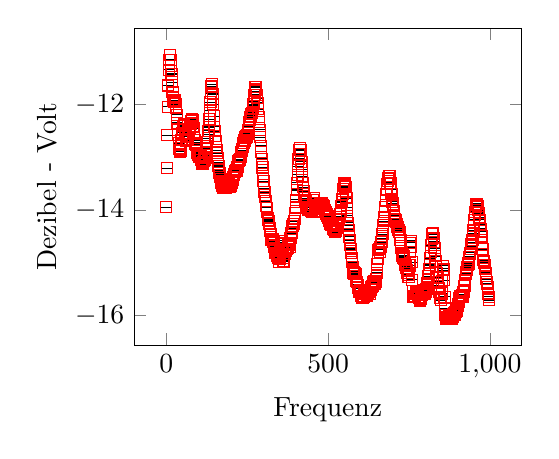
\begin{tikzpicture}
		\pgfplotsset{width=6.5cm,compat=1.3,legend style={font=\footnotesize}}
		\begin{axis}[xlabel={Frequenz},ylabel={Dezibel - Volt},legend cell align=left,legend pos=north west]
		\addplot+[only marks,color=red,mark=square,error bars/.cd,x dir=both,x explicit,y dir=both,y explicit,error bar style={color=black}] table[x=X,y=Y,x error=xerror,y error=yerror,row sep=\\]{			X	Y	xerror	yerror	\\			0.0	-13.942701	0	0	\\			1.464844	-13.204845	0	0	\\			2.929687	-12.576747	0	0	\\			4.394531	-12.043003	0	0	\\			5.859375	-11.637319	0	0	\\			7.324219	-11.338841	0	0	\\			8.789062	-11.147334	0	0	\\			10.253906	-11.055148	0	0	\\			11.71875	-11.052612	0	0	\\			13.183594	-11.147603	0	0	\\			14.648437	-11.264567	0	0	\\			16.113281	-11.420076	0	0	\\			17.578125	-11.576912	0	0	\\			19.042969	-11.754877	0	0	\\			20.507812	-11.865007	0	0	\\			21.972656	-11.935255	0	0	\\			23.4375	-11.951572	0	0	\\			24.902344	-11.921883	0	0	\\			26.367187	-11.929547	0	0	\\			27.832031	-11.957509	0	0	\\			29.296875	-11.988999	0	0	\\			30.761719	-12.054073	0	0	\\			32.226562	-12.190961	0	0	\\			33.691406	-12.340184	0	0	\\			35.15625	-12.471862	0	0	\\			36.621094	-12.576409	0	0	\\			38.085937	-12.735684	0	0	\\			39.550781	-12.830654	0	0	\\			41.015625	-12.858981	0	0	\\			42.480469	-12.886751	0	0	\\			43.945312	-12.873018	0	0	\\			45.410156	-12.757756	0	0	\\			46.875	-12.672141	0	0	\\			48.339844	-12.577644	0	0	\\			49.804687	-12.533662	0	0	\\			51.269531	-12.470544	0	0	\\			52.734375	-12.403929	0	0	\\			54.199219	-12.378011	0	0	\\			55.664062	-12.359871	0	0	\\			57.128906	-12.40629	0	0	\\			58.59375	-12.533058	0	0	\\			60.058594	-12.597598	0	0	\\			61.523437	-12.679656	0	0	\\			62.988281	-12.67373	0	0	\\			64.453125	-12.651316	0	0	\\			65.917969	-12.643628	0	0	\\			67.382812	-12.611623	0	0	\\			68.847656	-12.558288	0	0	\\			70.3125	-12.534953	0	0	\\			71.777344	-12.459117	0	0	\\			73.242187	-12.435655	0	0	\\			74.707031	-12.370071	0	0	\\			76.171875	-12.344978	0	0	\\			77.636719	-12.318837	0	0	\\			79.101562	-12.279436	0	0	\\			80.566406	-12.29228	0	0	\\			82.03125	-12.402502	0	0	\\			83.496094	-12.430204	0	0	\\			84.960937	-12.453233	0	0	\\			86.425781	-12.535659	0	0	\\			87.890625	-12.676308	0	0	\\			89.355469	-12.751915	0	0	\\			90.820312	-12.723668	0	0	\\			92.285156	-12.765617	0	0	\\			93.75	-12.842001	0	0	\\			95.214844	-12.915969	0	0	\\			96.679687	-12.96026	0	0	\\			98.144531	-12.958488	0	0	\\			99.609375	-12.953785	0	0	\\			101.074219	-12.975211	0	0	\\			102.539062	-12.989285	0	0	\\			104.003906	-12.96097	0	0	\\			105.46875	-12.960481	0	0	\\			106.933594	-12.985016	0	0	\\			108.398437	-13.047441	0	0	\\			109.863281	-13.101651	0	0	\\			111.328125	-13.126928	0	0	\\			112.792969	-13.120827	0	0	\\			114.257812	-13.094006	0	0	\\			115.722656	-13.056845	0	0	\\			117.1875	-13.001685	0	0	\\			118.652344	-13.016473	0	0	\\			120.117187	-13.045897	0	0	\\			121.582031	-12.956312	0	0	\\			123.046875	-12.897386	0	0	\\			124.511719	-12.827514	0	0	\\			125.976562	-12.71386	0	0	\\			127.441406	-12.637093	0	0	\\			128.90625	-12.573133	0	0	\\			130.371094	-12.497792	0	0	\\			131.835937	-12.423589	0	0	\\			133.300781	-12.279614	0	0	\\			134.765625	-12.112174	0	0	\\			136.230469	-11.954012	0	0	\\			137.695312	-11.782011	0	0	\\			139.160156	-11.655701	0	0	\\			140.625	-11.613642	0	0	\\			142.089844	-11.670149	0	0	\\			143.554687	-11.797521	0	0	\\			145.019531	-11.993061	0	0	\\			146.484375	-12.220146	0	0	\\			147.949219	-12.419225	0	0	\\			149.414062	-12.507267	0	0	\\			150.878906	-12.598077	0	0	\\			152.34375	-12.691319	0	0	\\			153.808594	-12.807975	0	0	\\			155.273437	-12.865136	0	0	\\			156.738281	-12.9162	0	0	\\			158.203125	-13.012534	0	0	\\			159.667969	-13.088484	0	0	\\			161.132812	-13.162894	0	0	\\			162.597656	-13.246654	0	0	\\			164.0625	-13.292014	0	0	\\			165.527344	-13.326068	0	0	\\			166.992187	-13.368197	0	0	\\			168.457031	-13.415468	0	0	\\			169.921875	-13.483186	0	0	\\			171.386719	-13.527621	0	0	\\			172.851562	-13.545442	0	0	\\			174.316406	-13.55872	0	0	\\			175.78125	-13.580776	0	0	\\			177.246094	-13.547524	0	0	\\			178.710937	-13.505181	0	0	\\			180.175781	-13.505351	0	0	\\			181.640625	-13.578564	0	0	\\			183.105469	-13.584041	0	0	\\			184.570312	-13.568674	0	0	\\			186.035156	-13.49667	0	0	\\			187.5	-13.494674	0	0	\\			188.964844	-13.483797	0	0	\\			190.429687	-13.477939	0	0	\\			191.894531	-13.495815	0	0	\\			193.359375	-13.537626	0	0	\\			194.824219	-13.559084	0	0	\\			196.289062	-13.555896	0	0	\\			197.753906	-13.525508	0	0	\\			199.21875	-13.54347	0	0	\\			200.683594	-13.524117	0	0	\\			202.148437	-13.488736	0	0	\\			203.613281	-13.456023	0	0	\\			205.078125	-13.430794	0	0	\\			206.542969	-13.370785	0	0	\\			208.007812	-13.317475	0	0	\\			209.472656	-13.335371	0	0	\\			210.9375	-13.273367	0	0	\\			212.402344	-13.251994	0	0	\\			213.867187	-13.251799	0	0	\\			215.332031	-13.24033	0	0	\\			216.796875	-13.238352	0	0	\\			218.261719	-13.249883	0	0	\\			219.726562	-13.181229	0	0	\\			221.191406	-13.094785	0	0	\\			222.65625	-13.073178	0	0	\\			224.121094	-13.046299	0	0	\\			225.585937	-13.062437	0	0	\\			227.050781	-13.050818	0	0	\\			228.515625	-13.036838	0	0	\\			229.980469	-12.986245	0	0	\\			231.445312	-12.900718	0	0	\\			232.910156	-12.871415	0	0	\\			234.375	-12.834026	0	0	\\			235.839844	-12.799475	0	0	\\			237.304687	-12.728813	0	0	\\			238.769531	-12.718642	0	0	\\			240.234375	-12.689222	0	0	\\			241.699219	-12.677824	0	0	\\			243.164062	-12.670021	0	0	\\			244.628906	-12.614446	0	0	\\			246.09375	-12.631316	0	0	\\			247.558594	-12.604908	0	0	\\			249.023437	-12.589565	0	0	\\			250.488281	-12.571904	0	0	\\			251.953125	-12.545929	0	0	\\			253.417969	-12.483469	0	0	\\			254.882812	-12.422483	0	0	\\			256.347656	-12.328643	0	0	\\			257.8125	-12.28886	0	0	\\			259.277344	-12.240373	0	0	\\			260.742187	-12.215986	0	0	\\			262.207031	-12.18516	0	0	\\			263.671875	-12.151876	0	0	\\			265.136719	-12.153231	0	0	\\			266.601562	-12.067989	0	0	\\			268.066406	-12.024238	0	0	\\			269.53125	-11.992	0	0	\\			270.996094	-11.938563	0	0	\\			272.460937	-11.817675	0	0	\\			273.925781	-11.746685	0	0	\\			275.390625	-11.666444	0	0	\\			276.855469	-11.664938	0	0	\\			278.320312	-11.713956	0	0	\\			279.785156	-11.817823	0	0	\\			281.25	-11.875142	0	0	\\			282.714844	-11.966791	0	0	\\			284.179687	-12.084998	0	0	\\			285.644531	-12.229042	0	0	\\			287.109375	-12.330758	0	0	\\			288.574219	-12.477256	0	0	\\			290.039062	-12.620622	0	0	\\			291.503906	-12.776725	0	0	\\			292.96875	-12.891323	0	0	\\			294.433594	-13.029192	0	0	\\			295.898437	-13.14196	0	0	\\			297.363281	-13.19	0	0	\\			298.828125	-13.312075	0	0	\\			300.292969	-13.453938	0	0	\\			301.757812	-13.583755	0	0	\\			303.222656	-13.660656	0	0	\\			304.6875	-13.717198	0	0	\\			306.152344	-13.7563	0	0	\\			307.617187	-13.826937	0	0	\\			309.082031	-13.921494	0	0	\\			310.546875	-13.954372	0	0	\\			312.011719	-14.037625	0	0	\\			313.476562	-14.151063	0	0	\\			314.941406	-14.186613	0	0	\\			316.40625	-14.207322	0	0	\\			317.871094	-14.254597	0	0	\\			319.335937	-14.341994	0	0	\\			320.800781	-14.398789	0	0	\\			322.265625	-14.458733	0	0	\\			323.730469	-14.516859	0	0	\\			325.195312	-14.557667	0	0	\\			326.660156	-14.56753	0	0	\\			328.125	-14.557977	0	0	\\			329.589844	-14.547275	0	0	\\			331.054687	-14.593855	0	0	\\			332.519531	-14.628416	0	0	\\			333.984375	-14.686758	0	0	\\			335.449219	-14.768237	0	0	\\			336.914062	-14.816406	0	0	\\			338.378906	-14.811687	0	0	\\			339.84375	-14.809983	0	0	\\			341.308594	-14.84328	0	0	\\			342.773437	-14.870665	0	0	\\			344.238281	-14.888765	0	0	\\			345.703125	-14.897768	0	0	\\			347.167969	-14.900529	0	0	\\			348.632812	-14.973273	0	0	\\			350.097656	-14.931808	0	0	\\			351.5625	-14.831406	0	0	\\			353.027344	-14.730088	0	0	\\			354.492187	-14.615507	0	0	\\			355.957031	-14.579196	0	0	\\			357.421875	-14.644941	0	0	\\			358.886719	-14.757033	0	0	\\			360.351562	-14.907507	0	0	\\			361.816406	-14.978758	0	0	\\			363.28125	-14.959956	0	0	\\			364.746094	-14.908538	0	0	\\			366.210937	-14.829733	0	0	\\			367.675781	-14.79724	0	0	\\			369.140625	-14.763604	0	0	\\			370.605469	-14.750956	0	0	\\			372.070312	-14.740303	0	0	\\			373.535156	-14.741837	0	0	\\			375.0	-14.70553	0	0	\\			376.464844	-14.654656	0	0	\\			377.929687	-14.625118	0	0	\\			379.394531	-14.649865	0	0	\\			380.859375	-14.688305	0	0	\\			382.324219	-14.627755	0	0	\\			383.789062	-14.523986	0	0	\\			385.253906	-14.43882	0	0	\\			386.71875	-14.433422	0	0	\\			388.183594	-14.348682	0	0	\\			389.648437	-14.30524	0	0	\\			391.113281	-14.302965	0	0	\\			392.578125	-14.254566	0	0	\\			394.042969	-14.258134	0	0	\\			395.507812	-14.20393	0	0	\\			396.972656	-14.16057	0	0	\\			398.4375	-14.052094	0	0	\\			399.902344	-13.949053	0	0	\\			401.367187	-13.799419	0	0	\\			402.832031	-13.618076	0	0	\\			404.296875	-13.481807	0	0	\\			405.761719	-13.329754	0	0	\\			407.226562	-13.169362	0	0	\\			408.691406	-13.030575	0	0	\\			410.15625	-12.936599	0	0	\\			411.621094	-12.863524	0	0	\\			413.085937	-12.825793	0	0	\\			414.550781	-12.859131	0	0	\\			416.015625	-12.944199	0	0	\\			417.480469	-13.081183	0	0	\\			418.945312	-13.22492	0	0	\\			420.410156	-13.370934	0	0	\\			421.875	-13.480241	0	0	\\			423.339844	-13.56253	0	0	\\			424.804687	-13.640199	0	0	\\			426.269531	-13.737966	0	0	\\			427.734375	-13.771365	0	0	\\			429.199219	-13.817863	0	0	\\			430.664062	-13.831241	0	0	\\			432.128906	-13.894872	0	0	\\			433.59375	-13.899959	0	0	\\			435.058594	-13.899149	0	0	\\			436.523437	-13.93678	0	0	\\			437.988281	-13.990607	0	0	\\			439.453125	-13.996391	0	0	\\			440.917969	-13.95257	0	0	\\			442.382812	-13.953011	0	0	\\			443.847656	-13.93915	0	0	\\			445.3125	-13.97926	0	0	\\			446.777344	-14.006657	0	0	\\			448.242187	-14.002872	0	0	\\			449.707031	-14.026813	0	0	\\			451.171875	-13.991538	0	0	\\			452.636719	-13.906338	0	0	\\			454.101562	-13.803005	0	0	\\			455.566406	-13.771182	0	0	\\			457.03125	-13.81324	0	0	\\			458.496094	-13.859787	0	0	\\			459.960937	-13.939184	0	0	\\			461.425781	-13.969916	0	0	\\			462.890625	-14.010095	0	0	\\			464.355469	-14.02604	0	0	\\			465.820312	-14.014759	0	0	\\			467.285156	-14.025878	0	0	\\			468.75	-14.019736	0	0	\\			470.214844	-13.982672	0	0	\\			471.679687	-13.936664	0	0	\\			473.144531	-13.918379	0	0	\\			474.609375	-13.887167	0	0	\\			476.074219	-13.866555	0	0	\\			477.539062	-13.900276	0	0	\\			479.003906	-13.891856	0	0	\\			480.46875	-13.878141	0	0	\\			481.933594	-13.872251	0	0	\\			483.398437	-13.899301	0	0	\\			484.863281	-13.925096	0	0	\\			486.328125	-13.926833	0	0	\\			487.792969	-13.964467	0	0	\\			489.257812	-13.993724	0	0	\\			490.722656	-13.995873	0	0	\\			492.1875	-14.029584	0	0	\\			493.652344	-14.055915	0	0	\\			495.117187	-14.077138	0	0	\\			496.582031	-14.083096	0	0	\\			498.046875	-14.10655	0	0	\\			499.511719	-14.110208	0	0	\\			500.976562	-14.137574	0	0	\\			502.441406	-14.163034	0	0	\\			503.90625	-14.195672	0	0	\\			505.371094	-14.258957	0	0	\\			506.835937	-14.251043	0	0	\\			508.300781	-14.259809	0	0	\\			509.765625	-14.277299	0	0	\\			511.230469	-14.287127	0	0	\\			512.695312	-14.273346	0	0	\\			514.160156	-14.287627	0	0	\\			515.625	-14.351435	0	0	\\			517.089844	-14.34561	0	0	\\			518.554687	-14.382638	0	0	\\			520.019531	-14.418221	0	0	\\			521.484375	-14.388119	0	0	\\			522.949219	-14.362593	0	0	\\			524.414062	-14.391473	0	0	\\			525.878906	-14.338644	0	0	\\			527.34375	-14.266886	0	0	\\			528.808594	-14.271313	0	0	\\			530.273437	-14.294716	0	0	\\			531.738281	-14.252988	0	0	\\			533.203125	-14.180993	0	0	\\			534.667969	-14.170244	0	0	\\			536.132812	-14.123275	0	0	\\			537.597656	-14.079428	0	0	\\			539.0625	-14.02577	0	0	\\			540.527344	-13.928225	0	0	\\			541.992187	-13.845215	0	0	\\			543.457031	-13.79485	0	0	\\			544.921875	-13.693807	0	0	\\			546.386719	-13.591373	0	0	\\			547.851562	-13.546019	0	0	\\			549.316406	-13.493517	0	0	\\			550.78125	-13.494599	0	0	\\			552.246094	-13.52621	0	0	\\			553.710937	-13.564783	0	0	\\			555.175781	-13.645352	0	0	\\			556.640625	-13.772658	0	0	\\			558.105469	-13.956159	0	0	\\			559.570312	-14.10543	0	0	\\			561.035156	-14.235673	0	0	\\			562.5	-14.294742	0	0	\\			563.964844	-14.375012	0	0	\\			565.429687	-14.499689	0	0	\\			566.894531	-14.565875	0	0	\\			568.359375	-14.66267	0	0	\\			569.824219	-14.735004	0	0	\\			571.289062	-14.81043	0	0	\\			572.753906	-14.915409	0	0	\\			574.21875	-14.985424	0	0	\\			575.683594	-15.074864	0	0	\\			577.148437	-15.160001	0	0	\\			578.613281	-15.195379	0	0	\\			580.078125	-15.168275	0	0	\\			581.542969	-15.212967	0	0	\\			583.007812	-15.194615	0	0	\\			584.472656	-15.213531	0	0	\\			585.9375	-15.251164	0	0	\\			587.402344	-15.343804	0	0	\\			588.867187	-15.355197	0	0	\\			590.332031	-15.355059	0	0	\\			591.796875	-15.410407	0	0	\\			593.261719	-15.474997	0	0	\\			594.726562	-15.535676	0	0	\\			596.191406	-15.540559	0	0	\\			597.65625	-15.515728	0	0	\\			599.121094	-15.518412	0	0	\\			600.585937	-15.569966	0	0	\\			602.050781	-15.626404	0	0	\\			603.515625	-15.629481	0	0	\\			604.980469	-15.648831	0	0	\\			606.445312	-15.660181	0	0	\\			607.910156	-15.637631	0	0	\\			609.375	-15.632234	0	0	\\			610.839844	-15.651203	0	0	\\			612.304687	-15.59054	0	0	\\			613.769531	-15.554668	0	0	\\			615.234375	-15.53164	0	0	\\			616.699219	-15.547696	0	0	\\			618.164062	-15.587611	0	0	\\			619.628906	-15.631271	0	0	\\			621.09375	-15.604856	0	0	\\			622.558594	-15.576629	0	0	\\			624.023437	-15.554948	0	0	\\			625.488281	-15.547817	0	0	\\			626.953125	-15.548004	0	0	\\			628.417969	-15.584139	0	0	\\			629.882812	-15.585855	0	0	\\			631.347656	-15.511413	0	0	\\			632.8125	-15.495455	0	0	\\			634.277344	-15.458992	0	0	\\			635.742187	-15.457001	0	0	\\			637.207031	-15.443464	0	0	\\			638.671875	-15.409661	0	0	\\			640.136719	-15.369919	0	0	\\			641.601562	-15.368311	0	0	\\			643.066406	-15.33513	0	0	\\			644.53125	-15.370836	0	0	\\			645.996094	-15.392783	0	0	\\			647.460937	-15.352274	0	0	\\			648.925781	-15.299623	0	0	\\			650.390625	-15.18584	0	0	\\			651.855469	-15.027185	0	0	\\			653.320312	-14.915233	0	0	\\			654.785156	-14.748179	0	0	\\			656.25	-14.729636	0	0	\\			657.714844	-14.7376	0	0	\\			659.179687	-14.793866	0	0	\\			660.644531	-14.79395	0	0	\\			662.109375	-14.694947	0	0	\\			663.574219	-14.610436	0	0	\\			665.039062	-14.605801	0	0	\\			666.503906	-14.534849	0	0	\\			667.96875	-14.456074	0	0	\\			669.433594	-14.384861	0	0	\\			670.898437	-14.274717	0	0	\\			672.363281	-14.210781	0	0	\\			673.828125	-14.132579	0	0	\\			675.292969	-14.026048	0	0	\\			676.757812	-13.932575	0	0	\\			678.222656	-13.80205	0	0	\\			679.6875	-13.696042	0	0	\\			681.152344	-13.611229	0	0	\\			682.617187	-13.496905	0	0	\\			684.082031	-13.453078	0	0	\\			685.546875	-13.387033	0	0	\\			687.011719	-13.385221	0	0	\\			688.476562	-13.347759	0	0	\\			689.941406	-13.346763	0	0	\\			691.40625	-13.404208	0	0	\\			692.871094	-13.479772	0	0	\\			694.335937	-13.598803	0	0	\\			695.800781	-13.69103	0	0	\\			697.265625	-13.792449	0	0	\\			698.730469	-13.836306	0	0	\\			700.195312	-13.874466	0	0	\\			701.660156	-13.914486	0	0	\\			703.125	-14.012992	0	0	\\			704.589844	-14.108539	0	0	\\			706.054687	-14.183387	0	0	\\			707.519531	-14.176331	0	0	\\			708.984375	-14.194716	0	0	\\			710.449219	-14.227381	0	0	\\			711.914062	-14.268867	0	0	\\			713.378906	-14.308342	0	0	\\			714.84375	-14.319887	0	0	\\			716.308594	-14.347137	0	0	\\			717.773437	-14.371882	0	0	\\			719.238281	-14.377188	0	0	\\			720.703125	-14.418471	0	0	\\			722.167969	-14.474339	0	0	\\			723.632812	-14.569186	0	0	\\			725.097656	-14.619404	0	0	\\			726.5625	-14.71305	0	0	\\			728.027344	-14.814438	0	0	\\			729.492187	-14.865781	0	0	\\			730.957031	-14.905653	0	0	\\			732.421875	-14.858385	0	0	\\			733.886719	-14.877496	0	0	\\			735.351562	-14.928999	0	0	\\			736.816406	-15.015374	0	0	\\			738.28125	-15.043015	0	0	\\			739.746094	-15.059551	0	0	\\			741.210937	-15.095169	0	0	\\			742.675781	-15.14563	0	0	\\			744.140625	-15.128118	0	0	\\			745.605469	-15.192386	0	0	\\			747.070312	-15.220927	0	0	\\			748.535156	-15.259638	0	0	\\			750.0	-15.230832	0	0	\\			751.464844	-15.047355	0	0	\\			752.929687	-14.798202	0	0	\\			754.394531	-14.617036	0	0	\\			755.859375	-14.581404	0	0	\\			757.324219	-14.704774	0	0	\\			758.789062	-14.982999	0	0	\\			760.253906	-15.319669	0	0	\\			761.71875	-15.533472	0	0	\\			763.183594	-15.651223	0	0	\\			764.648437	-15.648231	0	0	\\			766.113281	-15.632652	0	0	\\			767.578125	-15.636229	0	0	\\			769.042969	-15.618493	0	0	\\			770.507812	-15.592191	0	0	\\			771.972656	-15.55513	0	0	\\			773.4375	-15.537814	0	0	\\			774.902344	-15.537207	0	0	\\			776.367187	-15.577723	0	0	\\			777.832031	-15.604742	0	0	\\			779.296875	-15.640573	0	0	\\			780.761719	-15.64904	0	0	\\			782.226562	-15.671233	0	0	\\			783.691406	-15.712063	0	0	\\			785.15625	-15.700436	0	0	\\			786.621094	-15.673309	0	0	\\			788.085937	-15.65391	0	0	\\			789.550781	-15.606123	0	0	\\			791.015625	-15.579804	0	0	\\			792.480469	-15.586203	0	0	\\			793.945312	-15.541138	0	0	\\			795.410156	-15.515093	0	0	\\			796.875	-15.536476	0	0	\\			798.339844	-15.560006	0	0	\\			799.804687	-15.578462	0	0	\\			801.269531	-15.540634	0	0	\\			802.734375	-15.497673	0	0	\\			804.199219	-15.491515	0	0	\\			805.664062	-15.476828	0	0	\\			807.128906	-15.383823	0	0	\\			808.59375	-15.312986	0	0	\\			810.058594	-15.25496	0	0	\\			811.523437	-15.199285	0	0	\\			812.988281	-15.107254	0	0	\\			814.453125	-15.037633	0	0	\\			815.917969	-14.913214	0	0	\\			817.382812	-14.795513	0	0	\\			818.847656	-14.659809	0	0	\\			820.3125	-14.542557	0	0	\\			821.777344	-14.455177	0	0	\\			823.242187	-14.441677	0	0	\\			824.707031	-14.452009	0	0	\\			826.171875	-14.523803	0	0	\\			827.636719	-14.601911	0	0	\\			829.101562	-14.72088	0	0	\\			830.566406	-14.872614	0	0	\\			832.03125	-14.964136	0	0	\\			833.496094	-15.060817	0	0	\\			834.960937	-15.186338	0	0	\\			836.425781	-15.266625	0	0	\\			837.890625	-15.289433	0	0	\\			839.355469	-15.359073	0	0	\\			840.820312	-15.42938	0	0	\\			842.285156	-15.472609	0	0	\\			843.75	-15.546187	0	0	\\			845.214844	-15.588039	0	0	\\			846.679687	-15.656313	0	0	\\			848.144531	-15.701602	0	0	\\			849.609375	-15.708706	0	0	\\			851.074219	-15.577674	0	0	\\			852.539062	-15.336022	0	0	\\			854.003906	-15.139862	0	0	\\			855.46875	-15.051172	0	0	\\			856.933594	-15.112661	0	0	\\			858.398437	-15.325623	0	0	\\			859.863281	-15.637842	0	0	\\			861.328125	-15.865741	0	0	\\			862.792969	-15.988279	0	0	\\			864.257812	-16.025916	0	0	\\			865.722656	-16.050948	0	0	\\			867.1875	-16.056271	0	0	\\			868.652344	-16.038009	0	0	\\			870.117187	-16.035544	0	0	\\			871.582031	-16.037216	0	0	\\			873.046875	-15.994429	0	0	\\			874.511719	-15.989459	0	0	\\			875.976562	-16.028235	0	0	\\			877.441406	-16.006544	0	0	\\			878.90625	-16.010197	0	0	\\			880.371094	-16.039067	0	0	\\			881.835937	-16.052858	0	0	\\			883.300781	-16.038819	0	0	\\			884.765625	-16.017636	0	0	\\			886.230469	-15.990222	0	0	\\			887.695312	-15.96821	0	0	\\			889.160156	-15.958759	0	0	\\			890.625	-15.956359	0	0	\\			892.089844	-15.989096	0	0	\\			893.554687	-15.931483	0	0	\\			895.019531	-15.897459	0	0	\\			896.484375	-15.901863	0	0	\\			897.949219	-15.904711	0	0	\\			899.414062	-15.854252	0	0	\\			900.878906	-15.813051	0	0	\\			902.34375	-15.773275	0	0	\\			903.808594	-15.74055	0	0	\\			905.273437	-15.671897	0	0	\\			906.738281	-15.638022	0	0	\\			908.203125	-15.628246	0	0	\\			909.667969	-15.633953	0	0	\\			911.132812	-15.636517	0	0	\\			912.597656	-15.618348	0	0	\\			914.0625	-15.606832	0	0	\\			915.527344	-15.642164	0	0	\\			916.992187	-15.60336	0	0	\\			918.457031	-15.557149	0	0	\\			919.921875	-15.504722	0	0	\\			921.386719	-15.433164	0	0	\\			922.851562	-15.40295	0	0	\\			924.316406	-15.320069	0	0	\\			925.78125	-15.207668	0	0	\\			927.246094	-15.175808	0	0	\\			928.710937	-15.133739	0	0	\\			930.175781	-15.075344	0	0	\\			931.640625	-15.04247	0	0	\\			933.105469	-15.001003	0	0	\\			934.570312	-15.009759	0	0	\\			936.035156	-14.887666	0	0	\\			937.5	-14.832107	0	0	\\			938.964844	-14.80857	0	0	\\			940.429687	-14.732576	0	0	\\			941.894531	-14.682797	0	0	\\			943.359375	-14.638536	0	0	\\			944.824219	-14.610377	0	0	\\			946.289062	-14.563308	0	0	\\			947.753906	-14.442696	0	0	\\			949.21875	-14.381956	0	0	\\			950.683594	-14.297972	0	0	\\			952.148437	-14.178126	0	0	\\			953.613281	-14.085948	0	0	\\			955.078125	-14.029816	0	0	\\			956.542969	-13.942281	0	0	\\			958.007812	-13.892934	0	0	\\			959.472656	-13.886662	0	0	\\			960.9375	-13.881844	0	0	\\			962.402344	-13.919304	0	0	\\			963.867187	-14.002444	0	0	\\			965.332031	-14.052671	0	0	\\			966.796875	-14.136698	0	0	\\			968.261719	-14.178512	0	0	\\			969.726562	-14.262606	0	0	\\			971.191406	-14.348539	0	0	\\			972.65625	-14.402612	0	0	\\			974.121094	-14.497048	0	0	\\			975.585937	-14.625538	0	0	\\			977.050781	-14.738054	0	0	\\			978.515625	-14.870678	0	0	\\			979.980469	-14.94646	0	0	\\			981.445312	-14.960288	0	0	\\			982.910156	-14.989767	0	0	\\			984.375	-15.047363	0	0	\\			985.839844	-15.110367	0	0	\\			987.304687	-15.189883	0	0	\\			988.769531	-15.303659	0	0	\\			990.234375	-15.353415	0	0	\\			991.699219	-15.392532	0	0	\\			993.164062	-15.463058	0	0	\\			994.628906	-15.578506	0	0	\\			996.09375	-15.639256	0	0	\\			997.558594	-15.700848	0	0	\\		};		% \addlegendentry{Messpunkte Datensatz 0}
		\end{axis}
		\end{tikzpicture}	\caption{Umgebung}
	\label{fig:Umgebungsmessung}\end{figure}
            \begin{figure}[H]
	\centering
	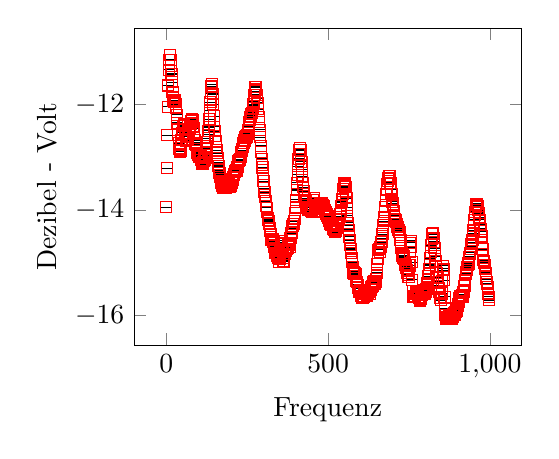
\begin{tikzpicture}
		\pgfplotsset{width=6.5cm,compat=1.3,legend style={font=\footnotesize}}
		\begin{axis}[xlabel={Frequenz},ylabel={Dezibel - Volt},legend cell align=left,legend pos=north west]
		\addplot+[only marks,color=red,mark=square,error bars/.cd,x dir=both,x explicit,y dir=both,y explicit,error bar style={color=black}] table[x=X,y=Y,x error=xerror,y error=yerror,row sep=\\]{			X	Y	xerror	yerror	\\			0.0	-13.942701	0	0	\\			1.464844	-13.204845	0	0	\\			2.929687	-12.576747	0	0	\\			4.394531	-12.043003	0	0	\\			5.859375	-11.637319	0	0	\\			7.324219	-11.338841	0	0	\\			8.789062	-11.147334	0	0	\\			10.253906	-11.055148	0	0	\\			11.71875	-11.052612	0	0	\\			13.183594	-11.147603	0	0	\\			14.648437	-11.264567	0	0	\\			16.113281	-11.420076	0	0	\\			17.578125	-11.576912	0	0	\\			19.042969	-11.754877	0	0	\\			20.507812	-11.865007	0	0	\\			21.972656	-11.935255	0	0	\\			23.4375	-11.951572	0	0	\\			24.902344	-11.921883	0	0	\\			26.367187	-11.929547	0	0	\\			27.832031	-11.957509	0	0	\\			29.296875	-11.988999	0	0	\\			30.761719	-12.054073	0	0	\\			32.226562	-12.190961	0	0	\\			33.691406	-12.340184	0	0	\\			35.15625	-12.471862	0	0	\\			36.621094	-12.576409	0	0	\\			38.085937	-12.735684	0	0	\\			39.550781	-12.830654	0	0	\\			41.015625	-12.858981	0	0	\\			42.480469	-12.886751	0	0	\\			43.945312	-12.873018	0	0	\\			45.410156	-12.757756	0	0	\\			46.875	-12.672141	0	0	\\			48.339844	-12.577644	0	0	\\			49.804687	-12.533662	0	0	\\			51.269531	-12.470544	0	0	\\			52.734375	-12.403929	0	0	\\			54.199219	-12.378011	0	0	\\			55.664062	-12.359871	0	0	\\			57.128906	-12.40629	0	0	\\			58.59375	-12.533058	0	0	\\			60.058594	-12.597598	0	0	\\			61.523437	-12.679656	0	0	\\			62.988281	-12.67373	0	0	\\			64.453125	-12.651316	0	0	\\			65.917969	-12.643628	0	0	\\			67.382812	-12.611623	0	0	\\			68.847656	-12.558288	0	0	\\			70.3125	-12.534953	0	0	\\			71.777344	-12.459117	0	0	\\			73.242187	-12.435655	0	0	\\			74.707031	-12.370071	0	0	\\			76.171875	-12.344978	0	0	\\			77.636719	-12.318837	0	0	\\			79.101562	-12.279436	0	0	\\			80.566406	-12.29228	0	0	\\			82.03125	-12.402502	0	0	\\			83.496094	-12.430204	0	0	\\			84.960937	-12.453233	0	0	\\			86.425781	-12.535659	0	0	\\			87.890625	-12.676308	0	0	\\			89.355469	-12.751915	0	0	\\			90.820312	-12.723668	0	0	\\			92.285156	-12.765617	0	0	\\			93.75	-12.842001	0	0	\\			95.214844	-12.915969	0	0	\\			96.679687	-12.96026	0	0	\\			98.144531	-12.958488	0	0	\\			99.609375	-12.953785	0	0	\\			101.074219	-12.975211	0	0	\\			102.539062	-12.989285	0	0	\\			104.003906	-12.96097	0	0	\\			105.46875	-12.960481	0	0	\\			106.933594	-12.985016	0	0	\\			108.398437	-13.047441	0	0	\\			109.863281	-13.101651	0	0	\\			111.328125	-13.126928	0	0	\\			112.792969	-13.120827	0	0	\\			114.257812	-13.094006	0	0	\\			115.722656	-13.056845	0	0	\\			117.1875	-13.001685	0	0	\\			118.652344	-13.016473	0	0	\\			120.117187	-13.045897	0	0	\\			121.582031	-12.956312	0	0	\\			123.046875	-12.897386	0	0	\\			124.511719	-12.827514	0	0	\\			125.976562	-12.71386	0	0	\\			127.441406	-12.637093	0	0	\\			128.90625	-12.573133	0	0	\\			130.371094	-12.497792	0	0	\\			131.835937	-12.423589	0	0	\\			133.300781	-12.279614	0	0	\\			134.765625	-12.112174	0	0	\\			136.230469	-11.954012	0	0	\\			137.695312	-11.782011	0	0	\\			139.160156	-11.655701	0	0	\\			140.625	-11.613642	0	0	\\			142.089844	-11.670149	0	0	\\			143.554687	-11.797521	0	0	\\			145.019531	-11.993061	0	0	\\			146.484375	-12.220146	0	0	\\			147.949219	-12.419225	0	0	\\			149.414062	-12.507267	0	0	\\			150.878906	-12.598077	0	0	\\			152.34375	-12.691319	0	0	\\			153.808594	-12.807975	0	0	\\			155.273437	-12.865136	0	0	\\			156.738281	-12.9162	0	0	\\			158.203125	-13.012534	0	0	\\			159.667969	-13.088484	0	0	\\			161.132812	-13.162894	0	0	\\			162.597656	-13.246654	0	0	\\			164.0625	-13.292014	0	0	\\			165.527344	-13.326068	0	0	\\			166.992187	-13.368197	0	0	\\			168.457031	-13.415468	0	0	\\			169.921875	-13.483186	0	0	\\			171.386719	-13.527621	0	0	\\			172.851562	-13.545442	0	0	\\			174.316406	-13.55872	0	0	\\			175.78125	-13.580776	0	0	\\			177.246094	-13.547524	0	0	\\			178.710937	-13.505181	0	0	\\			180.175781	-13.505351	0	0	\\			181.640625	-13.578564	0	0	\\			183.105469	-13.584041	0	0	\\			184.570312	-13.568674	0	0	\\			186.035156	-13.49667	0	0	\\			187.5	-13.494674	0	0	\\			188.964844	-13.483797	0	0	\\			190.429687	-13.477939	0	0	\\			191.894531	-13.495815	0	0	\\			193.359375	-13.537626	0	0	\\			194.824219	-13.559084	0	0	\\			196.289062	-13.555896	0	0	\\			197.753906	-13.525508	0	0	\\			199.21875	-13.54347	0	0	\\			200.683594	-13.524117	0	0	\\			202.148437	-13.488736	0	0	\\			203.613281	-13.456023	0	0	\\			205.078125	-13.430794	0	0	\\			206.542969	-13.370785	0	0	\\			208.007812	-13.317475	0	0	\\			209.472656	-13.335371	0	0	\\			210.9375	-13.273367	0	0	\\			212.402344	-13.251994	0	0	\\			213.867187	-13.251799	0	0	\\			215.332031	-13.24033	0	0	\\			216.796875	-13.238352	0	0	\\			218.261719	-13.249883	0	0	\\			219.726562	-13.181229	0	0	\\			221.191406	-13.094785	0	0	\\			222.65625	-13.073178	0	0	\\			224.121094	-13.046299	0	0	\\			225.585937	-13.062437	0	0	\\			227.050781	-13.050818	0	0	\\			228.515625	-13.036838	0	0	\\			229.980469	-12.986245	0	0	\\			231.445312	-12.900718	0	0	\\			232.910156	-12.871415	0	0	\\			234.375	-12.834026	0	0	\\			235.839844	-12.799475	0	0	\\			237.304687	-12.728813	0	0	\\			238.769531	-12.718642	0	0	\\			240.234375	-12.689222	0	0	\\			241.699219	-12.677824	0	0	\\			243.164062	-12.670021	0	0	\\			244.628906	-12.614446	0	0	\\			246.09375	-12.631316	0	0	\\			247.558594	-12.604908	0	0	\\			249.023437	-12.589565	0	0	\\			250.488281	-12.571904	0	0	\\			251.953125	-12.545929	0	0	\\			253.417969	-12.483469	0	0	\\			254.882812	-12.422483	0	0	\\			256.347656	-12.328643	0	0	\\			257.8125	-12.28886	0	0	\\			259.277344	-12.240373	0	0	\\			260.742187	-12.215986	0	0	\\			262.207031	-12.18516	0	0	\\			263.671875	-12.151876	0	0	\\			265.136719	-12.153231	0	0	\\			266.601562	-12.067989	0	0	\\			268.066406	-12.024238	0	0	\\			269.53125	-11.992	0	0	\\			270.996094	-11.938563	0	0	\\			272.460937	-11.817675	0	0	\\			273.925781	-11.746685	0	0	\\			275.390625	-11.666444	0	0	\\			276.855469	-11.664938	0	0	\\			278.320312	-11.713956	0	0	\\			279.785156	-11.817823	0	0	\\			281.25	-11.875142	0	0	\\			282.714844	-11.966791	0	0	\\			284.179687	-12.084998	0	0	\\			285.644531	-12.229042	0	0	\\			287.109375	-12.330758	0	0	\\			288.574219	-12.477256	0	0	\\			290.039062	-12.620622	0	0	\\			291.503906	-12.776725	0	0	\\			292.96875	-12.891323	0	0	\\			294.433594	-13.029192	0	0	\\			295.898437	-13.14196	0	0	\\			297.363281	-13.19	0	0	\\			298.828125	-13.312075	0	0	\\			300.292969	-13.453938	0	0	\\			301.757812	-13.583755	0	0	\\			303.222656	-13.660656	0	0	\\			304.6875	-13.717198	0	0	\\			306.152344	-13.7563	0	0	\\			307.617187	-13.826937	0	0	\\			309.082031	-13.921494	0	0	\\			310.546875	-13.954372	0	0	\\			312.011719	-14.037625	0	0	\\			313.476562	-14.151063	0	0	\\			314.941406	-14.186613	0	0	\\			316.40625	-14.207322	0	0	\\			317.871094	-14.254597	0	0	\\			319.335937	-14.341994	0	0	\\			320.800781	-14.398789	0	0	\\			322.265625	-14.458733	0	0	\\			323.730469	-14.516859	0	0	\\			325.195312	-14.557667	0	0	\\			326.660156	-14.56753	0	0	\\			328.125	-14.557977	0	0	\\			329.589844	-14.547275	0	0	\\			331.054687	-14.593855	0	0	\\			332.519531	-14.628416	0	0	\\			333.984375	-14.686758	0	0	\\			335.449219	-14.768237	0	0	\\			336.914062	-14.816406	0	0	\\			338.378906	-14.811687	0	0	\\			339.84375	-14.809983	0	0	\\			341.308594	-14.84328	0	0	\\			342.773437	-14.870665	0	0	\\			344.238281	-14.888765	0	0	\\			345.703125	-14.897768	0	0	\\			347.167969	-14.900529	0	0	\\			348.632812	-14.973273	0	0	\\			350.097656	-14.931808	0	0	\\			351.5625	-14.831406	0	0	\\			353.027344	-14.730088	0	0	\\			354.492187	-14.615507	0	0	\\			355.957031	-14.579196	0	0	\\			357.421875	-14.644941	0	0	\\			358.886719	-14.757033	0	0	\\			360.351562	-14.907507	0	0	\\			361.816406	-14.978758	0	0	\\			363.28125	-14.959956	0	0	\\			364.746094	-14.908538	0	0	\\			366.210937	-14.829733	0	0	\\			367.675781	-14.79724	0	0	\\			369.140625	-14.763604	0	0	\\			370.605469	-14.750956	0	0	\\			372.070312	-14.740303	0	0	\\			373.535156	-14.741837	0	0	\\			375.0	-14.70553	0	0	\\			376.464844	-14.654656	0	0	\\			377.929687	-14.625118	0	0	\\			379.394531	-14.649865	0	0	\\			380.859375	-14.688305	0	0	\\			382.324219	-14.627755	0	0	\\			383.789062	-14.523986	0	0	\\			385.253906	-14.43882	0	0	\\			386.71875	-14.433422	0	0	\\			388.183594	-14.348682	0	0	\\			389.648437	-14.30524	0	0	\\			391.113281	-14.302965	0	0	\\			392.578125	-14.254566	0	0	\\			394.042969	-14.258134	0	0	\\			395.507812	-14.20393	0	0	\\			396.972656	-14.16057	0	0	\\			398.4375	-14.052094	0	0	\\			399.902344	-13.949053	0	0	\\			401.367187	-13.799419	0	0	\\			402.832031	-13.618076	0	0	\\			404.296875	-13.481807	0	0	\\			405.761719	-13.329754	0	0	\\			407.226562	-13.169362	0	0	\\			408.691406	-13.030575	0	0	\\			410.15625	-12.936599	0	0	\\			411.621094	-12.863524	0	0	\\			413.085937	-12.825793	0	0	\\			414.550781	-12.859131	0	0	\\			416.015625	-12.944199	0	0	\\			417.480469	-13.081183	0	0	\\			418.945312	-13.22492	0	0	\\			420.410156	-13.370934	0	0	\\			421.875	-13.480241	0	0	\\			423.339844	-13.56253	0	0	\\			424.804687	-13.640199	0	0	\\			426.269531	-13.737966	0	0	\\			427.734375	-13.771365	0	0	\\			429.199219	-13.817863	0	0	\\			430.664062	-13.831241	0	0	\\			432.128906	-13.894872	0	0	\\			433.59375	-13.899959	0	0	\\			435.058594	-13.899149	0	0	\\			436.523437	-13.93678	0	0	\\			437.988281	-13.990607	0	0	\\			439.453125	-13.996391	0	0	\\			440.917969	-13.95257	0	0	\\			442.382812	-13.953011	0	0	\\			443.847656	-13.93915	0	0	\\			445.3125	-13.97926	0	0	\\			446.777344	-14.006657	0	0	\\			448.242187	-14.002872	0	0	\\			449.707031	-14.026813	0	0	\\			451.171875	-13.991538	0	0	\\			452.636719	-13.906338	0	0	\\			454.101562	-13.803005	0	0	\\			455.566406	-13.771182	0	0	\\			457.03125	-13.81324	0	0	\\			458.496094	-13.859787	0	0	\\			459.960937	-13.939184	0	0	\\			461.425781	-13.969916	0	0	\\			462.890625	-14.010095	0	0	\\			464.355469	-14.02604	0	0	\\			465.820312	-14.014759	0	0	\\			467.285156	-14.025878	0	0	\\			468.75	-14.019736	0	0	\\			470.214844	-13.982672	0	0	\\			471.679687	-13.936664	0	0	\\			473.144531	-13.918379	0	0	\\			474.609375	-13.887167	0	0	\\			476.074219	-13.866555	0	0	\\			477.539062	-13.900276	0	0	\\			479.003906	-13.891856	0	0	\\			480.46875	-13.878141	0	0	\\			481.933594	-13.872251	0	0	\\			483.398437	-13.899301	0	0	\\			484.863281	-13.925096	0	0	\\			486.328125	-13.926833	0	0	\\			487.792969	-13.964467	0	0	\\			489.257812	-13.993724	0	0	\\			490.722656	-13.995873	0	0	\\			492.1875	-14.029584	0	0	\\			493.652344	-14.055915	0	0	\\			495.117187	-14.077138	0	0	\\			496.582031	-14.083096	0	0	\\			498.046875	-14.10655	0	0	\\			499.511719	-14.110208	0	0	\\			500.976562	-14.137574	0	0	\\			502.441406	-14.163034	0	0	\\			503.90625	-14.195672	0	0	\\			505.371094	-14.258957	0	0	\\			506.835937	-14.251043	0	0	\\			508.300781	-14.259809	0	0	\\			509.765625	-14.277299	0	0	\\			511.230469	-14.287127	0	0	\\			512.695312	-14.273346	0	0	\\			514.160156	-14.287627	0	0	\\			515.625	-14.351435	0	0	\\			517.089844	-14.34561	0	0	\\			518.554687	-14.382638	0	0	\\			520.019531	-14.418221	0	0	\\			521.484375	-14.388119	0	0	\\			522.949219	-14.362593	0	0	\\			524.414062	-14.391473	0	0	\\			525.878906	-14.338644	0	0	\\			527.34375	-14.266886	0	0	\\			528.808594	-14.271313	0	0	\\			530.273437	-14.294716	0	0	\\			531.738281	-14.252988	0	0	\\			533.203125	-14.180993	0	0	\\			534.667969	-14.170244	0	0	\\			536.132812	-14.123275	0	0	\\			537.597656	-14.079428	0	0	\\			539.0625	-14.02577	0	0	\\			540.527344	-13.928225	0	0	\\			541.992187	-13.845215	0	0	\\			543.457031	-13.79485	0	0	\\			544.921875	-13.693807	0	0	\\			546.386719	-13.591373	0	0	\\			547.851562	-13.546019	0	0	\\			549.316406	-13.493517	0	0	\\			550.78125	-13.494599	0	0	\\			552.246094	-13.52621	0	0	\\			553.710937	-13.564783	0	0	\\			555.175781	-13.645352	0	0	\\			556.640625	-13.772658	0	0	\\			558.105469	-13.956159	0	0	\\			559.570312	-14.10543	0	0	\\			561.035156	-14.235673	0	0	\\			562.5	-14.294742	0	0	\\			563.964844	-14.375012	0	0	\\			565.429687	-14.499689	0	0	\\			566.894531	-14.565875	0	0	\\			568.359375	-14.66267	0	0	\\			569.824219	-14.735004	0	0	\\			571.289062	-14.81043	0	0	\\			572.753906	-14.915409	0	0	\\			574.21875	-14.985424	0	0	\\			575.683594	-15.074864	0	0	\\			577.148437	-15.160001	0	0	\\			578.613281	-15.195379	0	0	\\			580.078125	-15.168275	0	0	\\			581.542969	-15.212967	0	0	\\			583.007812	-15.194615	0	0	\\			584.472656	-15.213531	0	0	\\			585.9375	-15.251164	0	0	\\			587.402344	-15.343804	0	0	\\			588.867187	-15.355197	0	0	\\			590.332031	-15.355059	0	0	\\			591.796875	-15.410407	0	0	\\			593.261719	-15.474997	0	0	\\			594.726562	-15.535676	0	0	\\			596.191406	-15.540559	0	0	\\			597.65625	-15.515728	0	0	\\			599.121094	-15.518412	0	0	\\			600.585937	-15.569966	0	0	\\			602.050781	-15.626404	0	0	\\			603.515625	-15.629481	0	0	\\			604.980469	-15.648831	0	0	\\			606.445312	-15.660181	0	0	\\			607.910156	-15.637631	0	0	\\			609.375	-15.632234	0	0	\\			610.839844	-15.651203	0	0	\\			612.304687	-15.59054	0	0	\\			613.769531	-15.554668	0	0	\\			615.234375	-15.53164	0	0	\\			616.699219	-15.547696	0	0	\\			618.164062	-15.587611	0	0	\\			619.628906	-15.631271	0	0	\\			621.09375	-15.604856	0	0	\\			622.558594	-15.576629	0	0	\\			624.023437	-15.554948	0	0	\\			625.488281	-15.547817	0	0	\\			626.953125	-15.548004	0	0	\\			628.417969	-15.584139	0	0	\\			629.882812	-15.585855	0	0	\\			631.347656	-15.511413	0	0	\\			632.8125	-15.495455	0	0	\\			634.277344	-15.458992	0	0	\\			635.742187	-15.457001	0	0	\\			637.207031	-15.443464	0	0	\\			638.671875	-15.409661	0	0	\\			640.136719	-15.369919	0	0	\\			641.601562	-15.368311	0	0	\\			643.066406	-15.33513	0	0	\\			644.53125	-15.370836	0	0	\\			645.996094	-15.392783	0	0	\\			647.460937	-15.352274	0	0	\\			648.925781	-15.299623	0	0	\\			650.390625	-15.18584	0	0	\\			651.855469	-15.027185	0	0	\\			653.320312	-14.915233	0	0	\\			654.785156	-14.748179	0	0	\\			656.25	-14.729636	0	0	\\			657.714844	-14.7376	0	0	\\			659.179687	-14.793866	0	0	\\			660.644531	-14.79395	0	0	\\			662.109375	-14.694947	0	0	\\			663.574219	-14.610436	0	0	\\			665.039062	-14.605801	0	0	\\			666.503906	-14.534849	0	0	\\			667.96875	-14.456074	0	0	\\			669.433594	-14.384861	0	0	\\			670.898437	-14.274717	0	0	\\			672.363281	-14.210781	0	0	\\			673.828125	-14.132579	0	0	\\			675.292969	-14.026048	0	0	\\			676.757812	-13.932575	0	0	\\			678.222656	-13.80205	0	0	\\			679.6875	-13.696042	0	0	\\			681.152344	-13.611229	0	0	\\			682.617187	-13.496905	0	0	\\			684.082031	-13.453078	0	0	\\			685.546875	-13.387033	0	0	\\			687.011719	-13.385221	0	0	\\			688.476562	-13.347759	0	0	\\			689.941406	-13.346763	0	0	\\			691.40625	-13.404208	0	0	\\			692.871094	-13.479772	0	0	\\			694.335937	-13.598803	0	0	\\			695.800781	-13.69103	0	0	\\			697.265625	-13.792449	0	0	\\			698.730469	-13.836306	0	0	\\			700.195312	-13.874466	0	0	\\			701.660156	-13.914486	0	0	\\			703.125	-14.012992	0	0	\\			704.589844	-14.108539	0	0	\\			706.054687	-14.183387	0	0	\\			707.519531	-14.176331	0	0	\\			708.984375	-14.194716	0	0	\\			710.449219	-14.227381	0	0	\\			711.914062	-14.268867	0	0	\\			713.378906	-14.308342	0	0	\\			714.84375	-14.319887	0	0	\\			716.308594	-14.347137	0	0	\\			717.773437	-14.371882	0	0	\\			719.238281	-14.377188	0	0	\\			720.703125	-14.418471	0	0	\\			722.167969	-14.474339	0	0	\\			723.632812	-14.569186	0	0	\\			725.097656	-14.619404	0	0	\\			726.5625	-14.71305	0	0	\\			728.027344	-14.814438	0	0	\\			729.492187	-14.865781	0	0	\\			730.957031	-14.905653	0	0	\\			732.421875	-14.858385	0	0	\\			733.886719	-14.877496	0	0	\\			735.351562	-14.928999	0	0	\\			736.816406	-15.015374	0	0	\\			738.28125	-15.043015	0	0	\\			739.746094	-15.059551	0	0	\\			741.210937	-15.095169	0	0	\\			742.675781	-15.14563	0	0	\\			744.140625	-15.128118	0	0	\\			745.605469	-15.192386	0	0	\\			747.070312	-15.220927	0	0	\\			748.535156	-15.259638	0	0	\\			750.0	-15.230832	0	0	\\			751.464844	-15.047355	0	0	\\			752.929687	-14.798202	0	0	\\			754.394531	-14.617036	0	0	\\			755.859375	-14.581404	0	0	\\			757.324219	-14.704774	0	0	\\			758.789062	-14.982999	0	0	\\			760.253906	-15.319669	0	0	\\			761.71875	-15.533472	0	0	\\			763.183594	-15.651223	0	0	\\			764.648437	-15.648231	0	0	\\			766.113281	-15.632652	0	0	\\			767.578125	-15.636229	0	0	\\			769.042969	-15.618493	0	0	\\			770.507812	-15.592191	0	0	\\			771.972656	-15.55513	0	0	\\			773.4375	-15.537814	0	0	\\			774.902344	-15.537207	0	0	\\			776.367187	-15.577723	0	0	\\			777.832031	-15.604742	0	0	\\			779.296875	-15.640573	0	0	\\			780.761719	-15.64904	0	0	\\			782.226562	-15.671233	0	0	\\			783.691406	-15.712063	0	0	\\			785.15625	-15.700436	0	0	\\			786.621094	-15.673309	0	0	\\			788.085937	-15.65391	0	0	\\			789.550781	-15.606123	0	0	\\			791.015625	-15.579804	0	0	\\			792.480469	-15.586203	0	0	\\			793.945312	-15.541138	0	0	\\			795.410156	-15.515093	0	0	\\			796.875	-15.536476	0	0	\\			798.339844	-15.560006	0	0	\\			799.804687	-15.578462	0	0	\\			801.269531	-15.540634	0	0	\\			802.734375	-15.497673	0	0	\\			804.199219	-15.491515	0	0	\\			805.664062	-15.476828	0	0	\\			807.128906	-15.383823	0	0	\\			808.59375	-15.312986	0	0	\\			810.058594	-15.25496	0	0	\\			811.523437	-15.199285	0	0	\\			812.988281	-15.107254	0	0	\\			814.453125	-15.037633	0	0	\\			815.917969	-14.913214	0	0	\\			817.382812	-14.795513	0	0	\\			818.847656	-14.659809	0	0	\\			820.3125	-14.542557	0	0	\\			821.777344	-14.455177	0	0	\\			823.242187	-14.441677	0	0	\\			824.707031	-14.452009	0	0	\\			826.171875	-14.523803	0	0	\\			827.636719	-14.601911	0	0	\\			829.101562	-14.72088	0	0	\\			830.566406	-14.872614	0	0	\\			832.03125	-14.964136	0	0	\\			833.496094	-15.060817	0	0	\\			834.960937	-15.186338	0	0	\\			836.425781	-15.266625	0	0	\\			837.890625	-15.289433	0	0	\\			839.355469	-15.359073	0	0	\\			840.820312	-15.42938	0	0	\\			842.285156	-15.472609	0	0	\\			843.75	-15.546187	0	0	\\			845.214844	-15.588039	0	0	\\			846.679687	-15.656313	0	0	\\			848.144531	-15.701602	0	0	\\			849.609375	-15.708706	0	0	\\			851.074219	-15.577674	0	0	\\			852.539062	-15.336022	0	0	\\			854.003906	-15.139862	0	0	\\			855.46875	-15.051172	0	0	\\			856.933594	-15.112661	0	0	\\			858.398437	-15.325623	0	0	\\			859.863281	-15.637842	0	0	\\			861.328125	-15.865741	0	0	\\			862.792969	-15.988279	0	0	\\			864.257812	-16.025916	0	0	\\			865.722656	-16.050948	0	0	\\			867.1875	-16.056271	0	0	\\			868.652344	-16.038009	0	0	\\			870.117187	-16.035544	0	0	\\			871.582031	-16.037216	0	0	\\			873.046875	-15.994429	0	0	\\			874.511719	-15.989459	0	0	\\			875.976562	-16.028235	0	0	\\			877.441406	-16.006544	0	0	\\			878.90625	-16.010197	0	0	\\			880.371094	-16.039067	0	0	\\			881.835937	-16.052858	0	0	\\			883.300781	-16.038819	0	0	\\			884.765625	-16.017636	0	0	\\			886.230469	-15.990222	0	0	\\			887.695312	-15.96821	0	0	\\			889.160156	-15.958759	0	0	\\			890.625	-15.956359	0	0	\\			892.089844	-15.989096	0	0	\\			893.554687	-15.931483	0	0	\\			895.019531	-15.897459	0	0	\\			896.484375	-15.901863	0	0	\\			897.949219	-15.904711	0	0	\\			899.414062	-15.854252	0	0	\\			900.878906	-15.813051	0	0	\\			902.34375	-15.773275	0	0	\\			903.808594	-15.74055	0	0	\\			905.273437	-15.671897	0	0	\\			906.738281	-15.638022	0	0	\\			908.203125	-15.628246	0	0	\\			909.667969	-15.633953	0	0	\\			911.132812	-15.636517	0	0	\\			912.597656	-15.618348	0	0	\\			914.0625	-15.606832	0	0	\\			915.527344	-15.642164	0	0	\\			916.992187	-15.60336	0	0	\\			918.457031	-15.557149	0	0	\\			919.921875	-15.504722	0	0	\\			921.386719	-15.433164	0	0	\\			922.851562	-15.40295	0	0	\\			924.316406	-15.320069	0	0	\\			925.78125	-15.207668	0	0	\\			927.246094	-15.175808	0	0	\\			928.710937	-15.133739	0	0	\\			930.175781	-15.075344	0	0	\\			931.640625	-15.04247	0	0	\\			933.105469	-15.001003	0	0	\\			934.570312	-15.009759	0	0	\\			936.035156	-14.887666	0	0	\\			937.5	-14.832107	0	0	\\			938.964844	-14.80857	0	0	\\			940.429687	-14.732576	0	0	\\			941.894531	-14.682797	0	0	\\			943.359375	-14.638536	0	0	\\			944.824219	-14.610377	0	0	\\			946.289062	-14.563308	0	0	\\			947.753906	-14.442696	0	0	\\			949.21875	-14.381956	0	0	\\			950.683594	-14.297972	0	0	\\			952.148437	-14.178126	0	0	\\			953.613281	-14.085948	0	0	\\			955.078125	-14.029816	0	0	\\			956.542969	-13.942281	0	0	\\			958.007812	-13.892934	0	0	\\			959.472656	-13.886662	0	0	\\			960.9375	-13.881844	0	0	\\			962.402344	-13.919304	0	0	\\			963.867187	-14.002444	0	0	\\			965.332031	-14.052671	0	0	\\			966.796875	-14.136698	0	0	\\			968.261719	-14.178512	0	0	\\			969.726562	-14.262606	0	0	\\			971.191406	-14.348539	0	0	\\			972.65625	-14.402612	0	0	\\			974.121094	-14.497048	0	0	\\			975.585937	-14.625538	0	0	\\			977.050781	-14.738054	0	0	\\			978.515625	-14.870678	0	0	\\			979.980469	-14.94646	0	0	\\			981.445312	-14.960288	0	0	\\			982.910156	-14.989767	0	0	\\			984.375	-15.047363	0	0	\\			985.839844	-15.110367	0	0	\\			987.304687	-15.189883	0	0	\\			988.769531	-15.303659	0	0	\\			990.234375	-15.353415	0	0	\\			991.699219	-15.392532	0	0	\\			993.164062	-15.463058	0	0	\\			994.628906	-15.578506	0	0	\\			996.09375	-15.639256	0	0	\\			997.558594	-15.700848	0	0	\\		};		% \addlegendentry{Messpunkte Datensatz 0}
		\end{axis}
		\end{tikzpicture}	\caption{Umgebung}
	\label{fig:Umgebungsmessung}\end{figure}
        
        \subsubsection*{31 degrees}
            \begin{table}[H]
	\centering
	\begin{tabular}{cccccc}
		$\nu$ & c & C(c) & $\kappa$ & f\\
		\hline
		0.0 & 11.0(50) & 22.0(22) & 21.9(219) & 0.01(00) & -2.02(-02)	\\
		1.0 & 142.0(50) & 142.0(142) & 141.83(1418) & 0.36(004) & -3.1(-031)	\\
		2.0 & 275.0(50) & 183.33(1833) & 183.17(1832) & 0.59(006) & -4.91(-049)	\\
		3.0 & 412.0(50) & 206.0(206) & 205.85(2059) & 0.75(007) & -7.96(-08)	\\
		4.0 & 550.0(50) & 220.0(220) & 219.86(2199) & 0.85(009) & -13.7(-137)	\\
		5.0 & 685.0(50) & 228.33(2283) & 228.21(2282) & 0.92(009) & -24.96(-25)	\\
		6.0 & 821.0(50) & 234.57(2346) & 234.45(2345) & 0.97(01) & -68.58(-686)	\\
		7.0 & 955.0(50) & 238.75(2388) & 238.64(2386) & 1.01(01) & 348.84(3488)	\\
		0.0(00) & 481.38(177) & 184.37(695) & 184.24(695) & 0.68(003) & 27.95(446)	\\
	\end{tabular}
\end{table}
            \begin{table}[H]
	\centering
	\begin{tabular}{cccccc}
		$\nu$ & c & C(c) & $\kappa$ & f\\
		\hline
		0.0 & 11.0(50) & 22.0(22) & 21.9(219) & 0.01(00) & -2.02(-02)	\\
		1.0 & 142.0(50) & 142.0(142) & 141.83(1418) & 0.36(004) & -3.1(-031)	\\
		2.0 & 275.0(50) & 183.33(1833) & 183.17(1832) & 0.59(006) & -4.91(-049)	\\
		3.0 & 412.0(50) & 206.0(206) & 205.85(2059) & 0.75(007) & -7.96(-08)	\\
		4.0 & 550.0(50) & 220.0(220) & 219.86(2199) & 0.85(009) & -13.7(-137)	\\
		5.0 & 685.0(50) & 228.33(2283) & 228.21(2282) & 0.92(009) & -24.96(-25)	\\
		6.0 & 821.0(50) & 234.57(2346) & 234.45(2345) & 0.97(01) & -68.58(-686)	\\
		7.0 & 955.0(50) & 238.75(2388) & 238.64(2386) & 1.01(01) & 348.84(3488)	\\
		0.0(00) & 481.38(177) & 184.37(695) & 184.24(695) & 0.68(003) & 27.95(446)	\\
	\end{tabular}
\end{table}

        \subsubsection*{15 degrees}
            \begin{figure}[H]
	\centering
	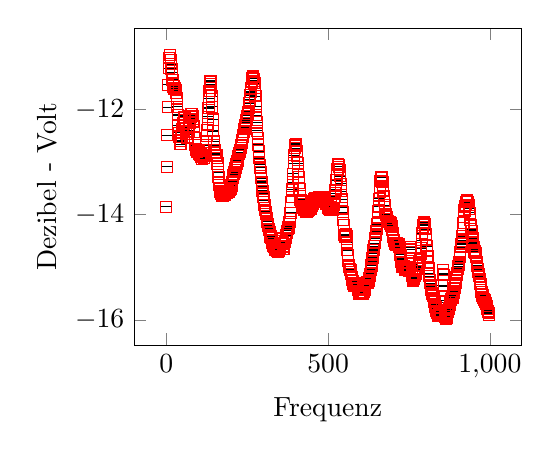
\begin{tikzpicture}
		\pgfplotsset{width=6.5cm,compat=1.3,legend style={font=\footnotesize}}
		\begin{axis}[xlabel={Frequenz},ylabel={Dezibel - Volt},legend cell align=left,legend pos=north west]
		\addplot+[only marks,color=red,mark=square,error bars/.cd,x dir=both,x explicit,y dir=both,y explicit,error bar style={color=black}] table[x=X,y=Y,x error=xerror,y error=yerror,row sep=\\]{			X	Y	xerror	yerror	\\			0.0	-13.845637	0	0	\\			1.464844	-13.088928	0	0	\\			2.929687	-12.487552	0	0	\\			4.394531	-11.956193	0	0	\\			5.859375	-11.532627	0	0	\\			7.324219	-11.219287	0	0	\\			8.789062	-11.029098	0	0	\\			10.253906	-10.959464	0	0	\\			11.71875	-10.963449	0	0	\\			13.183594	-11.064873	0	0	\\			14.648437	-11.139374	0	0	\\			16.113281	-11.231231	0	0	\\			17.578125	-11.306855	0	0	\\			19.042969	-11.441749	0	0	\\			20.507812	-11.509028	0	0	\\			21.972656	-11.564013	0	0	\\			23.4375	-11.599294	0	0	\\			24.902344	-11.611793	0	0	\\			26.367187	-11.59182	0	0	\\			27.832031	-11.597961	0	0	\\			29.296875	-11.633078	0	0	\\			30.761719	-11.688168	0	0	\\			32.226562	-11.792487	0	0	\\			33.691406	-11.947671	0	0	\\			35.15625	-12.105735	0	0	\\			36.621094	-12.296936	0	0	\\			38.085937	-12.440178	0	0	\\			39.550781	-12.52494	0	0	\\			41.015625	-12.590731	0	0	\\			42.480469	-12.664031	0	0	\\			43.945312	-12.659126	0	0	\\			45.410156	-12.600547	0	0	\\			46.875	-12.524998	0	0	\\			48.339844	-12.429365	0	0	\\			49.804687	-12.370833	0	0	\\			51.269531	-12.32125	0	0	\\			52.734375	-12.265648	0	0	\\			54.199219	-12.193185	0	0	\\			55.664062	-12.139367	0	0	\\			57.128906	-12.155751	0	0	\\			58.59375	-12.256134	0	0	\\			60.058594	-12.359106	0	0	\\			61.523437	-12.468442	0	0	\\			62.988281	-12.522492	0	0	\\			64.453125	-12.533764	0	0	\\			65.917969	-12.516911	0	0	\\			67.382812	-12.462909	0	0	\\			68.847656	-12.408586	0	0	\\			70.3125	-12.345712	0	0	\\			71.777344	-12.258651	0	0	\\			73.242187	-12.200916	0	0	\\			74.707031	-12.135249	0	0	\\			76.171875	-12.118023	0	0	\\			77.636719	-12.091574	0	0	\\			79.101562	-12.094173	0	0	\\			80.566406	-12.130064	0	0	\\			82.03125	-12.180158	0	0	\\			83.496094	-12.232008	0	0	\\			84.960937	-12.322847	0	0	\\			86.425781	-12.427347	0	0	\\			87.890625	-12.541159	0	0	\\			89.355469	-12.678436	0	0	\\			90.820312	-12.744004	0	0	\\			92.285156	-12.778161	0	0	\\			93.75	-12.815157	0	0	\\			95.214844	-12.815723	0	0	\\			96.679687	-12.791711	0	0	\\			98.144531	-12.793728	0	0	\\			99.609375	-12.787673	0	0	\\			101.074219	-12.79238	0	0	\\			102.539062	-12.838746	0	0	\\			104.003906	-12.837577	0	0	\\			105.46875	-12.854905	0	0	\\			106.933594	-12.866493	0	0	\\			108.398437	-12.894294	0	0	\\			109.863281	-12.934398	0	0	\\			111.328125	-12.909145	0	0	\\			112.792969	-12.880447	0	0	\\			114.257812	-12.878889	0	0	\\			115.722656	-12.887172	0	0	\\			117.1875	-12.92433	0	0	\\			118.652344	-12.874154	0	0	\\			120.117187	-12.771505	0	0	\\			121.582031	-12.683303	0	0	\\			123.046875	-12.6165	0	0	\\			124.511719	-12.498552	0	0	\\			125.976562	-12.393442	0	0	\\			127.441406	-12.285095	0	0	\\			128.90625	-12.137004	0	0	\\			130.371094	-11.97353	0	0	\\			131.835937	-11.796344	0	0	\\			133.300781	-11.648126	0	0	\\			134.765625	-11.520562	0	0	\\			136.230469	-11.453027	0	0	\\			137.695312	-11.469786	0	0	\\			139.160156	-11.585625	0	0	\\			140.625	-11.752429	0	0	\\			142.089844	-11.949923	0	0	\\			143.554687	-12.192667	0	0	\\			145.019531	-12.408609	0	0	\\			146.484375	-12.604097	0	0	\\			147.949219	-12.67586	0	0	\\			149.414062	-12.764159	0	0	\\			150.878906	-12.834516	0	0	\\			152.34375	-12.874702	0	0	\\			153.808594	-12.862474	0	0	\\			155.273437	-12.865949	0	0	\\			156.738281	-12.922241	0	0	\\			158.203125	-13.027744	0	0	\\			159.667969	-13.18746	0	0	\\			161.132812	-13.286355	0	0	\\			162.597656	-13.387026	0	0	\\			164.0625	-13.437584	0	0	\\			165.527344	-13.512292	0	0	\\			166.992187	-13.559034	0	0	\\			168.457031	-13.571206	0	0	\\			169.921875	-13.606499	0	0	\\			171.386719	-13.622466	0	0	\\			172.851562	-13.639717	0	0	\\			174.316406	-13.621648	0	0	\\			175.78125	-13.643245	0	0	\\			177.246094	-13.603829	0	0	\\			178.710937	-13.603671	0	0	\\			180.175781	-13.627501	0	0	\\			181.640625	-13.594675	0	0	\\			183.105469	-13.593166	0	0	\\			184.570312	-13.592601	0	0	\\			186.035156	-13.566002	0	0	\\			187.5	-13.579392	0	0	\\			188.964844	-13.563857	0	0	\\			190.429687	-13.55247	0	0	\\			191.894531	-13.560878	0	0	\\			193.359375	-13.56488	0	0	\\			194.824219	-13.57043	0	0	\\			196.289062	-13.534955	0	0	\\			197.753906	-13.500838	0	0	\\			199.21875	-13.513006	0	0	\\			200.683594	-13.507678	0	0	\\			202.148437	-13.44483	0	0	\\			203.613281	-13.370993	0	0	\\			205.078125	-13.291755	0	0	\\			206.542969	-13.247786	0	0	\\			208.007812	-13.227698	0	0	\\			209.472656	-13.194717	0	0	\\			210.9375	-13.182857	0	0	\\			212.402344	-13.154425	0	0	\\			213.867187	-13.117	0	0	\\			215.332031	-13.053043	0	0	\\			216.796875	-13.039621	0	0	\\			218.261719	-13.002926	0	0	\\			219.726562	-12.975222	0	0	\\			221.191406	-12.971189	0	0	\\			222.65625	-12.893127	0	0	\\			224.121094	-12.848768	0	0	\\			225.585937	-12.830488	0	0	\\			227.050781	-12.810252	0	0	\\			228.515625	-12.769749	0	0	\\			229.980469	-12.737457	0	0	\\			231.445312	-12.673939	0	0	\\			232.910156	-12.63381	0	0	\\			234.375	-12.574101	0	0	\\			235.839844	-12.527854	0	0	\\			237.304687	-12.481818	0	0	\\			238.769531	-12.430734	0	0	\\			240.234375	-12.427523	0	0	\\			241.699219	-12.370658	0	0	\\			243.164062	-12.34247	0	0	\\			244.628906	-12.303308	0	0	\\			246.09375	-12.258272	0	0	\\			247.558594	-12.201188	0	0	\\			249.023437	-12.165037	0	0	\\			250.488281	-12.119416	0	0	\\			251.953125	-12.077951	0	0	\\			253.417969	-12.046904	0	0	\\			254.882812	-11.965291	0	0	\\			256.347656	-11.884195	0	0	\\			257.8125	-11.815085	0	0	\\			259.277344	-11.732568	0	0	\\			260.742187	-11.668042	0	0	\\			262.207031	-11.589826	0	0	\\			263.671875	-11.469939	0	0	\\			265.136719	-11.398355	0	0	\\			266.601562	-11.365629	0	0	\\			268.066406	-11.387698	0	0	\\			269.53125	-11.419317	0	0	\\			270.996094	-11.452708	0	0	\\			272.460937	-11.502193	0	0	\\			273.925781	-11.600704	0	0	\\			275.390625	-11.74875	0	0	\\			276.855469	-11.944337	0	0	\\			278.320312	-12.112832	0	0	\\			279.785156	-12.24687	0	0	\\			281.25	-12.40685	0	0	\\			282.714844	-12.546097	0	0	\\			284.179687	-12.667338	0	0	\\			285.644531	-12.797778	0	0	\\			287.109375	-12.926696	0	0	\\			288.574219	-13.049757	0	0	\\			290.039062	-13.104293	0	0	\\			291.503906	-13.192661	0	0	\\			292.96875	-13.305774	0	0	\\			294.433594	-13.377486	0	0	\\			295.898437	-13.462044	0	0	\\			297.363281	-13.544584	0	0	\\			298.828125	-13.597206	0	0	\\			300.292969	-13.656481	0	0	\\			301.757812	-13.729157	0	0	\\			303.222656	-13.814649	0	0	\\			304.6875	-13.875941	0	0	\\			306.152344	-13.91417	0	0	\\			307.617187	-13.940508	0	0	\\			309.082031	-13.981872	0	0	\\			310.546875	-14.069664	0	0	\\			312.011719	-14.136594	0	0	\\			313.476562	-14.183375	0	0	\\			314.941406	-14.211977	0	0	\\			316.40625	-14.268102	0	0	\\			317.871094	-14.281854	0	0	\\			319.335937	-14.321448	0	0	\\			320.800781	-14.424588	0	0	\\			322.265625	-14.416637	0	0	\\			323.730469	-14.405082	0	0	\\			325.195312	-14.445088	0	0	\\			326.660156	-14.493321	0	0	\\			328.125	-14.539701	0	0	\\			329.589844	-14.569761	0	0	\\			331.054687	-14.598695	0	0	\\			332.519531	-14.617563	0	0	\\			333.984375	-14.611022	0	0	\\			335.449219	-14.629418	0	0	\\			336.914062	-14.67445	0	0	\\			338.378906	-14.665944	0	0	\\			339.84375	-14.663783	0	0	\\			341.308594	-14.662337	0	0	\\			342.773437	-14.694866	0	0	\\			344.238281	-14.70015	0	0	\\			345.703125	-14.670906	0	0	\\			347.167969	-14.678919	0	0	\\			348.632812	-14.670805	0	0	\\			350.097656	-14.64759	0	0	\\			351.5625	-14.601923	0	0	\\			353.027344	-14.541609	0	0	\\			354.492187	-14.492567	0	0	\\			355.957031	-14.437379	0	0	\\			357.421875	-14.454657	0	0	\\			358.886719	-14.529799	0	0	\\			360.351562	-14.618642	0	0	\\			361.816406	-14.657008	0	0	\\			363.28125	-14.600342	0	0	\\			364.746094	-14.549357	0	0	\\			366.210937	-14.521714	0	0	\\			367.675781	-14.511634	0	0	\\			369.140625	-14.447255	0	0	\\			370.605469	-14.392787	0	0	\\			372.070312	-14.343887	0	0	\\			373.535156	-14.306607	0	0	\\			375.0	-14.263527	0	0	\\			376.464844	-14.239838	0	0	\\			377.929687	-14.246036	0	0	\\			379.394531	-14.226116	0	0	\\			380.859375	-14.13885	0	0	\\			382.324219	-14.0737	0	0	\\			383.789062	-13.961833	0	0	\\			385.253906	-13.86584	0	0	\\			386.71875	-13.764702	0	0	\\			388.183594	-13.658588	0	0	\\			389.648437	-13.520819	0	0	\\			391.113281	-13.382753	0	0	\\			392.578125	-13.220636	0	0	\\			394.042969	-13.023833	0	0	\\			395.507812	-12.872331	0	0	\\			396.972656	-12.738782	0	0	\\			398.4375	-12.672557	0	0	\\			399.902344	-12.652175	0	0	\\			401.367187	-12.698905	0	0	\\			402.832031	-12.799086	0	0	\\			404.296875	-12.889607	0	0	\\			405.761719	-13.026336	0	0	\\			407.226562	-13.172597	0	0	\\			408.691406	-13.28465	0	0	\\			410.15625	-13.403685	0	0	\\			411.621094	-13.50574	0	0	\\			413.085937	-13.636359	0	0	\\			414.550781	-13.713899	0	0	\\			416.015625	-13.739324	0	0	\\			417.480469	-13.760428	0	0	\\			418.945312	-13.791074	0	0	\\			420.410156	-13.836168	0	0	\\			421.875	-13.833169	0	0	\\			423.339844	-13.867541	0	0	\\			424.804687	-13.893637	0	0	\\			426.269531	-13.912817	0	0	\\			427.734375	-13.899469	0	0	\\			429.199219	-13.906873	0	0	\\			430.664062	-13.951151	0	0	\\			432.128906	-13.923956	0	0	\\			433.59375	-13.944122	0	0	\\			435.058594	-13.94901	0	0	\\			436.523437	-13.923193	0	0	\\			437.988281	-13.90986	0	0	\\			439.453125	-13.898796	0	0	\\			440.917969	-13.89526	0	0	\\			442.382812	-13.890502	0	0	\\			443.847656	-13.882114	0	0	\\			445.3125	-13.890585	0	0	\\			446.777344	-13.845588	0	0	\\			448.242187	-13.823455	0	0	\\			449.707031	-13.823307	0	0	\\			451.171875	-13.826454	0	0	\\			452.636719	-13.799036	0	0	\\			454.101562	-13.740584	0	0	\\			455.566406	-13.710364	0	0	\\			457.03125	-13.698966	0	0	\\			458.496094	-13.698184	0	0	\\			459.960937	-13.684752	0	0	\\			461.425781	-13.694755	0	0	\\			462.890625	-13.710817	0	0	\\			464.355469	-13.74088	0	0	\\			465.820312	-13.739073	0	0	\\			467.285156	-13.71099	0	0	\\			468.75	-13.710598	0	0	\\			470.214844	-13.698179	0	0	\\			471.679687	-13.656016	0	0	\\			473.144531	-13.663707	0	0	\\			474.609375	-13.679641	0	0	\\			476.074219	-13.695893	0	0	\\			477.539062	-13.709278	0	0	\\			479.003906	-13.721452	0	0	\\			480.46875	-13.713698	0	0	\\			481.933594	-13.683888	0	0	\\			483.398437	-13.665434	0	0	\\			484.863281	-13.685424	0	0	\\			486.328125	-13.701349	0	0	\\			487.792969	-13.725251	0	0	\\			489.257812	-13.758379	0	0	\\			490.722656	-13.76059	0	0	\\			492.1875	-13.781702	0	0	\\			493.652344	-13.792537	0	0	\\			495.117187	-13.782774	0	0	\\			496.582031	-13.787396	0	0	\\			498.046875	-13.790169	0	0	\\			499.511719	-13.833128	0	0	\\			500.976562	-13.875599	0	0	\\			502.441406	-13.875272	0	0	\\			503.90625	-13.88249	0	0	\\			505.371094	-13.906617	0	0	\\			506.835937	-13.89051	0	0	\\			508.300781	-13.891451	0	0	\\			509.765625	-13.859818	0	0	\\			511.230469	-13.887908	0	0	\\			512.695312	-13.875347	0	0	\\			514.160156	-13.908144	0	0	\\			515.625	-13.866448	0	0	\\			517.089844	-13.821797	0	0	\\			518.554687	-13.771138	0	0	\\			520.019531	-13.663214	0	0	\\			521.484375	-13.58927	0	0	\\			522.949219	-13.526482	0	0	\\			524.414062	-13.435181	0	0	\\			525.878906	-13.345335	0	0	\\			527.34375	-13.227726	0	0	\\			528.808594	-13.125322	0	0	\\			530.273437	-13.048815	0	0	\\			531.738281	-13.032181	0	0	\\			533.203125	-13.053213	0	0	\\			534.667969	-13.091407	0	0	\\			536.132812	-13.151154	0	0	\\			537.597656	-13.26802	0	0	\\			539.0625	-13.413139	0	0	\\			540.527344	-13.556576	0	0	\\			541.992187	-13.711031	0	0	\\			543.457031	-13.866082	0	0	\\			544.921875	-13.954423	0	0	\\			546.386719	-14.090817	0	0	\\			547.851562	-14.199237	0	0	\\			549.316406	-14.31676	0	0	\\			550.78125	-14.391369	0	0	\\			552.246094	-14.426841	0	0	\\			553.710937	-14.411461	0	0	\\			555.175781	-14.367005	0	0	\\			556.640625	-14.409225	0	0	\\			558.105469	-14.526983	0	0	\\			559.570312	-14.669581	0	0	\\			561.035156	-14.773026	0	0	\\			562.5	-14.873155	0	0	\\			563.964844	-14.948347	0	0	\\			565.429687	-14.990159	0	0	\\			566.894531	-15.024158	0	0	\\			568.359375	-15.046155	0	0	\\			569.824219	-15.055378	0	0	\\			571.289062	-15.129112	0	0	\\			572.753906	-15.191021	0	0	\\			574.21875	-15.240018	0	0	\\			575.683594	-15.256951	0	0	\\			577.148437	-15.266799	0	0	\\			578.613281	-15.305396	0	0	\\			580.078125	-15.335981	0	0	\\			581.542969	-15.350168	0	0	\\			583.007812	-15.342511	0	0	\\			584.472656	-15.354838	0	0	\\			585.9375	-15.345438	0	0	\\			587.402344	-15.328204	0	0	\\			588.867187	-15.324493	0	0	\\			590.332031	-15.342323	0	0	\\			591.796875	-15.386828	0	0	\\			593.261719	-15.418557	0	0	\\			594.726562	-15.473182	0	0	\\			596.191406	-15.495535	0	0	\\			597.65625	-15.474763	0	0	\\			599.121094	-15.471118	0	0	\\			600.585937	-15.495993	0	0	\\			602.050781	-15.4939	0	0	\\			603.515625	-15.492875	0	0	\\			604.980469	-15.495026	0	0	\\			606.445312	-15.511254	0	0	\\			607.910156	-15.480713	0	0	\\			609.375	-15.463784	0	0	\\			610.839844	-15.461015	0	0	\\			612.304687	-15.431714	0	0	\\			613.769531	-15.396537	0	0	\\			615.234375	-15.353024	0	0	\\			616.699219	-15.300741	0	0	\\			618.164062	-15.302895	0	0	\\			619.628906	-15.286069	0	0	\\			621.09375	-15.290201	0	0	\\			622.558594	-15.292723	0	0	\\			624.023437	-15.278993	0	0	\\			625.488281	-15.250444	0	0	\\			626.953125	-15.209255	0	0	\\			628.417969	-15.169875	0	0	\\			629.882812	-15.126041	0	0	\\			631.347656	-15.045888	0	0	\\			632.8125	-15.021813	0	0	\\			634.277344	-14.964118	0	0	\\			635.742187	-14.897492	0	0	\\			637.207031	-14.816599	0	0	\\			638.671875	-14.732306	0	0	\\			640.136719	-14.674813	0	0	\\			641.601562	-14.66396	0	0	\\			643.066406	-14.601937	0	0	\\			644.53125	-14.539907	0	0	\\			645.996094	-14.452773	0	0	\\			647.460937	-14.376739	0	0	\\			648.925781	-14.318162	0	0	\\			650.390625	-14.26842	0	0	\\			651.855469	-14.184245	0	0	\\			653.320312	-14.05194	0	0	\\			654.785156	-13.936842	0	0	\\			656.25	-13.843489	0	0	\\			657.714844	-13.69973	0	0	\\			659.179687	-13.572372	0	0	\\			660.644531	-13.466685	0	0	\\			662.109375	-13.354409	0	0	\\			663.574219	-13.278289	0	0	\\			665.039062	-13.285216	0	0	\\			666.503906	-13.298134	0	0	\\			667.96875	-13.371205	0	0	\\			669.433594	-13.46064	0	0	\\			670.898437	-13.540956	0	0	\\			672.363281	-13.64094	0	0	\\			673.828125	-13.744583	0	0	\\			675.292969	-13.819179	0	0	\\			676.757812	-13.942559	0	0	\\			678.222656	-13.979875	0	0	\\			679.6875	-13.996332	0	0	\\			681.152344	-14.044094	0	0	\\			682.617187	-14.082489	0	0	\\			684.082031	-14.118431	0	0	\\			685.546875	-14.135459	0	0	\\			687.011719	-14.130839	0	0	\\			688.476562	-14.132049	0	0	\\			689.941406	-14.13603	0	0	\\			691.40625	-14.15073	0	0	\\			692.871094	-14.165595	0	0	\\			694.335937	-14.184282	0	0	\\			695.800781	-14.214667	0	0	\\			697.265625	-14.23889	0	0	\\			698.730469	-14.282096	0	0	\\			700.195312	-14.340217	0	0	\\			701.660156	-14.427696	0	0	\\			703.125	-14.480946	0	0	\\			704.589844	-14.506445	0	0	\\			706.054687	-14.543649	0	0	\\			707.519531	-14.55167	0	0	\\			708.984375	-14.563492	0	0	\\			710.449219	-14.549737	0	0	\\			711.914062	-14.551367	0	0	\\			713.378906	-14.54375	0	0	\\			714.84375	-14.547964	0	0	\\			716.308594	-14.555533	0	0	\\			717.773437	-14.552491	0	0	\\			719.238281	-14.583339	0	0	\\			720.703125	-14.612525	0	0	\\			722.167969	-14.683572	0	0	\\			723.632812	-14.760236	0	0	\\			725.097656	-14.840779	0	0	\\			726.5625	-14.890059	0	0	\\			728.027344	-14.923745	0	0	\\			729.492187	-14.986367	0	0	\\			730.957031	-14.982654	0	0	\\			732.421875	-14.974218	0	0	\\			733.886719	-14.979483	0	0	\\			735.351562	-14.994169	0	0	\\			736.816406	-15.017811	0	0	\\			738.28125	-15.049903	0	0	\\			739.746094	-15.022716	0	0	\\			741.210937	-15.008058	0	0	\\			742.675781	-14.998375	0	0	\\			744.140625	-15.010212	0	0	\\			745.605469	-15.036397	0	0	\\			747.070312	-15.02963	0	0	\\			748.535156	-15.040693	0	0	\\			750.0	-15.058834	0	0	\\			751.464844	-15.009312	0	0	\\			752.929687	-14.835641	0	0	\\			754.394531	-14.660726	0	0	\\			755.859375	-14.620354	0	0	\\			757.324219	-14.713556	0	0	\\			758.789062	-14.939033	0	0	\\			760.253906	-15.152754	0	0	\\			761.71875	-15.246144	0	0	\\			763.183594	-15.26326	0	0	\\			764.648437	-15.218464	0	0	\\			766.113281	-15.19029	0	0	\\			767.578125	-15.167702	0	0	\\			769.042969	-15.118996	0	0	\\			770.507812	-15.119777	0	0	\\			771.972656	-15.074538	0	0	\\			773.4375	-15.032429	0	0	\\			774.902344	-15.009126	0	0	\\			776.367187	-15.02908	0	0	\\			777.832031	-15.028686	0	0	\\			779.296875	-15.019706	0	0	\\			780.761719	-14.975439	0	0	\\			782.226562	-14.907924	0	0	\\			783.691406	-14.864333	0	0	\\			785.15625	-14.822957	0	0	\\			786.621094	-14.735079	0	0	\\			788.085937	-14.630975	0	0	\\			789.550781	-14.482886	0	0	\\			791.015625	-14.347175	0	0	\\			792.480469	-14.238613	0	0	\\			793.945312	-14.201431	0	0	\\			795.410156	-14.150437	0	0	\\			796.875	-14.148655	0	0	\\			798.339844	-14.186322	0	0	\\			799.804687	-14.271598	0	0	\\			801.269531	-14.371493	0	0	\\			802.734375	-14.469272	0	0	\\			804.199219	-14.594962	0	0	\\			805.664062	-14.676923	0	0	\\			807.128906	-14.785405	0	0	\\			808.59375	-14.904512	0	0	\\			810.058594	-15.022046	0	0	\\			811.523437	-15.118098	0	0	\\			812.988281	-15.164744	0	0	\\			814.453125	-15.236771	0	0	\\			815.917969	-15.29937	0	0	\\			817.382812	-15.364021	0	0	\\			818.847656	-15.436604	0	0	\\			820.3125	-15.487332	0	0	\\			821.777344	-15.512645	0	0	\\			823.242187	-15.515715	0	0	\\			824.707031	-15.536379	0	0	\\			826.171875	-15.583069	0	0	\\			827.636719	-15.610482	0	0	\\			829.101562	-15.651435	0	0	\\			830.566406	-15.71404	0	0	\\			832.03125	-15.745797	0	0	\\			833.496094	-15.771859	0	0	\\			834.960937	-15.830697	0	0	\\			836.425781	-15.845988	0	0	\\			837.890625	-15.868136	0	0	\\			839.355469	-15.923388	0	0	\\			840.820312	-15.902677	0	0	\\			842.285156	-15.891028	0	0	\\			843.75	-15.865521	0	0	\\			845.214844	-15.86314	0	0	\\			846.679687	-15.879326	0	0	\\			848.144531	-15.885238	0	0	\\			849.609375	-15.842066	0	0	\\			851.074219	-15.633384	0	0	\\			852.539062	-15.338244	0	0	\\			854.003906	-15.117716	0	0	\\			855.46875	-15.047679	0	0	\\			856.933594	-15.137861	0	0	\\			858.398437	-15.359499	0	0	\\			859.863281	-15.660651	0	0	\\			861.328125	-15.867598	0	0	\\			862.792969	-15.931939	0	0	\\			864.257812	-15.974505	0	0	\\			865.722656	-15.958823	0	0	\\			867.1875	-15.893917	0	0	\\			868.652344	-15.870512	0	0	\\			870.117187	-15.842193	0	0	\\			871.582031	-15.807583	0	0	\\			873.046875	-15.796905	0	0	\\			874.511719	-15.78061	0	0	\\			875.976562	-15.72174	0	0	\\			877.441406	-15.662604	0	0	\\			878.90625	-15.616526	0	0	\\			880.371094	-15.598947	0	0	\\			881.835937	-15.586359	0	0	\\			883.300781	-15.586643	0	0	\\			884.765625	-15.574417	0	0	\\			886.230469	-15.533836	0	0	\\			887.695312	-15.492554	0	0	\\			889.160156	-15.455023	0	0	\\			890.625	-15.396705	0	0	\\			892.089844	-15.33625	0	0	\\			893.554687	-15.294342	0	0	\\			895.019531	-15.254466	0	0	\\			896.484375	-15.19195	0	0	\\			897.949219	-15.147596	0	0	\\			899.414062	-15.104964	0	0	\\			900.878906	-15.025797	0	0	\\			902.34375	-14.979203	0	0	\\			903.808594	-14.945298	0	0	\\			905.273437	-14.892065	0	0	\\			906.738281	-14.810202	0	0	\\			908.203125	-14.699769	0	0	\\			909.667969	-14.620296	0	0	\\			911.132812	-14.557624	0	0	\\			912.597656	-14.546026	0	0	\\			914.0625	-14.491136	0	0	\\			915.527344	-14.411666	0	0	\\			916.992187	-14.26002	0	0	\\			918.457031	-14.15248	0	0	\\			919.921875	-14.040175	0	0	\\			921.386719	-13.919137	0	0	\\			922.851562	-13.858676	0	0	\\			924.316406	-13.838256	0	0	\\			925.78125	-13.811635	0	0	\\			927.246094	-13.763359	0	0	\\			928.710937	-13.734589	0	0	\\			930.175781	-13.713536	0	0	\\			931.640625	-13.751364	0	0	\\			933.105469	-13.757202	0	0	\\			934.570312	-13.812546	0	0	\\			936.035156	-13.883219	0	0	\\			937.5	-13.963227	0	0	\\			938.964844	-14.093413	0	0	\\			940.429687	-14.205605	0	0	\\			941.894531	-14.271766	0	0	\\			943.359375	-14.307276	0	0	\\			944.824219	-14.374094	0	0	\\			946.289062	-14.451861	0	0	\\			947.753906	-14.536043	0	0	\\			949.21875	-14.610933	0	0	\\			950.683594	-14.668919	0	0	\\			952.148437	-14.714284	0	0	\\			953.613281	-14.723504	0	0	\\			955.078125	-14.694765	0	0	\\			956.542969	-14.723559	0	0	\\			958.007812	-14.792506	0	0	\\			959.472656	-14.902854	0	0	\\			960.9375	-14.968658	0	0	\\			962.402344	-15.038511	0	0	\\			963.867187	-15.084668	0	0	\\			965.332031	-15.128245	0	0	\\			966.796875	-15.170732	0	0	\\			968.261719	-15.217479	0	0	\\			969.726562	-15.288583	0	0	\\			971.191406	-15.321499	0	0	\\			972.65625	-15.39301	0	0	\\			974.121094	-15.469708	0	0	\\			975.585937	-15.504325	0	0	\\			977.050781	-15.532072	0	0	\\			978.515625	-15.561975	0	0	\\			979.980469	-15.582893	0	0	\\			981.445312	-15.595799	0	0	\\			982.910156	-15.616026	0	0	\\			984.375	-15.611584	0	0	\\			985.839844	-15.654299	0	0	\\			987.304687	-15.682083	0	0	\\			988.769531	-15.691098	0	0	\\			990.234375	-15.733659	0	0	\\			991.699219	-15.789129	0	0	\\			993.164062	-15.828453	0	0	\\			994.628906	-15.85357	0	0	\\			996.09375	-15.873472	0	0	\\			997.558594	-15.897968	0	0	\\		};		% \addlegendentry{Messpunkte Datensatz 0}
		\end{axis}
		\end{tikzpicture}	\caption{Umgebung}
	\label{fig:Umgebungsmessung}\end{figure}
            \begin{figure}[H]
	\centering
	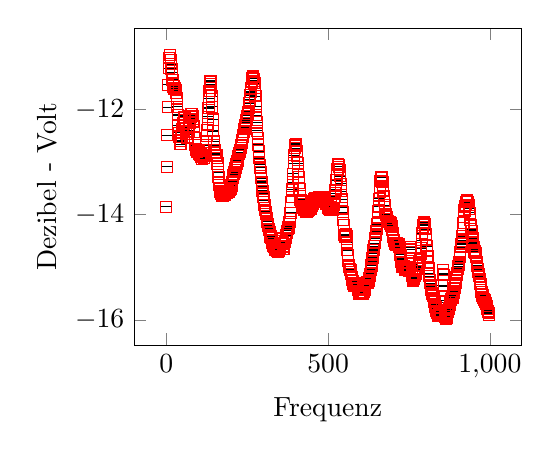
\begin{tikzpicture}
		\pgfplotsset{width=6.5cm,compat=1.3,legend style={font=\footnotesize}}
		\begin{axis}[xlabel={Frequenz},ylabel={Dezibel - Volt},legend cell align=left,legend pos=north west]
		\addplot+[only marks,color=red,mark=square,error bars/.cd,x dir=both,x explicit,y dir=both,y explicit,error bar style={color=black}] table[x=X,y=Y,x error=xerror,y error=yerror,row sep=\\]{			X	Y	xerror	yerror	\\			0.0	-13.845637	0	0	\\			1.464844	-13.088928	0	0	\\			2.929687	-12.487552	0	0	\\			4.394531	-11.956193	0	0	\\			5.859375	-11.532627	0	0	\\			7.324219	-11.219287	0	0	\\			8.789062	-11.029098	0	0	\\			10.253906	-10.959464	0	0	\\			11.71875	-10.963449	0	0	\\			13.183594	-11.064873	0	0	\\			14.648437	-11.139374	0	0	\\			16.113281	-11.231231	0	0	\\			17.578125	-11.306855	0	0	\\			19.042969	-11.441749	0	0	\\			20.507812	-11.509028	0	0	\\			21.972656	-11.564013	0	0	\\			23.4375	-11.599294	0	0	\\			24.902344	-11.611793	0	0	\\			26.367187	-11.59182	0	0	\\			27.832031	-11.597961	0	0	\\			29.296875	-11.633078	0	0	\\			30.761719	-11.688168	0	0	\\			32.226562	-11.792487	0	0	\\			33.691406	-11.947671	0	0	\\			35.15625	-12.105735	0	0	\\			36.621094	-12.296936	0	0	\\			38.085937	-12.440178	0	0	\\			39.550781	-12.52494	0	0	\\			41.015625	-12.590731	0	0	\\			42.480469	-12.664031	0	0	\\			43.945312	-12.659126	0	0	\\			45.410156	-12.600547	0	0	\\			46.875	-12.524998	0	0	\\			48.339844	-12.429365	0	0	\\			49.804687	-12.370833	0	0	\\			51.269531	-12.32125	0	0	\\			52.734375	-12.265648	0	0	\\			54.199219	-12.193185	0	0	\\			55.664062	-12.139367	0	0	\\			57.128906	-12.155751	0	0	\\			58.59375	-12.256134	0	0	\\			60.058594	-12.359106	0	0	\\			61.523437	-12.468442	0	0	\\			62.988281	-12.522492	0	0	\\			64.453125	-12.533764	0	0	\\			65.917969	-12.516911	0	0	\\			67.382812	-12.462909	0	0	\\			68.847656	-12.408586	0	0	\\			70.3125	-12.345712	0	0	\\			71.777344	-12.258651	0	0	\\			73.242187	-12.200916	0	0	\\			74.707031	-12.135249	0	0	\\			76.171875	-12.118023	0	0	\\			77.636719	-12.091574	0	0	\\			79.101562	-12.094173	0	0	\\			80.566406	-12.130064	0	0	\\			82.03125	-12.180158	0	0	\\			83.496094	-12.232008	0	0	\\			84.960937	-12.322847	0	0	\\			86.425781	-12.427347	0	0	\\			87.890625	-12.541159	0	0	\\			89.355469	-12.678436	0	0	\\			90.820312	-12.744004	0	0	\\			92.285156	-12.778161	0	0	\\			93.75	-12.815157	0	0	\\			95.214844	-12.815723	0	0	\\			96.679687	-12.791711	0	0	\\			98.144531	-12.793728	0	0	\\			99.609375	-12.787673	0	0	\\			101.074219	-12.79238	0	0	\\			102.539062	-12.838746	0	0	\\			104.003906	-12.837577	0	0	\\			105.46875	-12.854905	0	0	\\			106.933594	-12.866493	0	0	\\			108.398437	-12.894294	0	0	\\			109.863281	-12.934398	0	0	\\			111.328125	-12.909145	0	0	\\			112.792969	-12.880447	0	0	\\			114.257812	-12.878889	0	0	\\			115.722656	-12.887172	0	0	\\			117.1875	-12.92433	0	0	\\			118.652344	-12.874154	0	0	\\			120.117187	-12.771505	0	0	\\			121.582031	-12.683303	0	0	\\			123.046875	-12.6165	0	0	\\			124.511719	-12.498552	0	0	\\			125.976562	-12.393442	0	0	\\			127.441406	-12.285095	0	0	\\			128.90625	-12.137004	0	0	\\			130.371094	-11.97353	0	0	\\			131.835937	-11.796344	0	0	\\			133.300781	-11.648126	0	0	\\			134.765625	-11.520562	0	0	\\			136.230469	-11.453027	0	0	\\			137.695312	-11.469786	0	0	\\			139.160156	-11.585625	0	0	\\			140.625	-11.752429	0	0	\\			142.089844	-11.949923	0	0	\\			143.554687	-12.192667	0	0	\\			145.019531	-12.408609	0	0	\\			146.484375	-12.604097	0	0	\\			147.949219	-12.67586	0	0	\\			149.414062	-12.764159	0	0	\\			150.878906	-12.834516	0	0	\\			152.34375	-12.874702	0	0	\\			153.808594	-12.862474	0	0	\\			155.273437	-12.865949	0	0	\\			156.738281	-12.922241	0	0	\\			158.203125	-13.027744	0	0	\\			159.667969	-13.18746	0	0	\\			161.132812	-13.286355	0	0	\\			162.597656	-13.387026	0	0	\\			164.0625	-13.437584	0	0	\\			165.527344	-13.512292	0	0	\\			166.992187	-13.559034	0	0	\\			168.457031	-13.571206	0	0	\\			169.921875	-13.606499	0	0	\\			171.386719	-13.622466	0	0	\\			172.851562	-13.639717	0	0	\\			174.316406	-13.621648	0	0	\\			175.78125	-13.643245	0	0	\\			177.246094	-13.603829	0	0	\\			178.710937	-13.603671	0	0	\\			180.175781	-13.627501	0	0	\\			181.640625	-13.594675	0	0	\\			183.105469	-13.593166	0	0	\\			184.570312	-13.592601	0	0	\\			186.035156	-13.566002	0	0	\\			187.5	-13.579392	0	0	\\			188.964844	-13.563857	0	0	\\			190.429687	-13.55247	0	0	\\			191.894531	-13.560878	0	0	\\			193.359375	-13.56488	0	0	\\			194.824219	-13.57043	0	0	\\			196.289062	-13.534955	0	0	\\			197.753906	-13.500838	0	0	\\			199.21875	-13.513006	0	0	\\			200.683594	-13.507678	0	0	\\			202.148437	-13.44483	0	0	\\			203.613281	-13.370993	0	0	\\			205.078125	-13.291755	0	0	\\			206.542969	-13.247786	0	0	\\			208.007812	-13.227698	0	0	\\			209.472656	-13.194717	0	0	\\			210.9375	-13.182857	0	0	\\			212.402344	-13.154425	0	0	\\			213.867187	-13.117	0	0	\\			215.332031	-13.053043	0	0	\\			216.796875	-13.039621	0	0	\\			218.261719	-13.002926	0	0	\\			219.726562	-12.975222	0	0	\\			221.191406	-12.971189	0	0	\\			222.65625	-12.893127	0	0	\\			224.121094	-12.848768	0	0	\\			225.585937	-12.830488	0	0	\\			227.050781	-12.810252	0	0	\\			228.515625	-12.769749	0	0	\\			229.980469	-12.737457	0	0	\\			231.445312	-12.673939	0	0	\\			232.910156	-12.63381	0	0	\\			234.375	-12.574101	0	0	\\			235.839844	-12.527854	0	0	\\			237.304687	-12.481818	0	0	\\			238.769531	-12.430734	0	0	\\			240.234375	-12.427523	0	0	\\			241.699219	-12.370658	0	0	\\			243.164062	-12.34247	0	0	\\			244.628906	-12.303308	0	0	\\			246.09375	-12.258272	0	0	\\			247.558594	-12.201188	0	0	\\			249.023437	-12.165037	0	0	\\			250.488281	-12.119416	0	0	\\			251.953125	-12.077951	0	0	\\			253.417969	-12.046904	0	0	\\			254.882812	-11.965291	0	0	\\			256.347656	-11.884195	0	0	\\			257.8125	-11.815085	0	0	\\			259.277344	-11.732568	0	0	\\			260.742187	-11.668042	0	0	\\			262.207031	-11.589826	0	0	\\			263.671875	-11.469939	0	0	\\			265.136719	-11.398355	0	0	\\			266.601562	-11.365629	0	0	\\			268.066406	-11.387698	0	0	\\			269.53125	-11.419317	0	0	\\			270.996094	-11.452708	0	0	\\			272.460937	-11.502193	0	0	\\			273.925781	-11.600704	0	0	\\			275.390625	-11.74875	0	0	\\			276.855469	-11.944337	0	0	\\			278.320312	-12.112832	0	0	\\			279.785156	-12.24687	0	0	\\			281.25	-12.40685	0	0	\\			282.714844	-12.546097	0	0	\\			284.179687	-12.667338	0	0	\\			285.644531	-12.797778	0	0	\\			287.109375	-12.926696	0	0	\\			288.574219	-13.049757	0	0	\\			290.039062	-13.104293	0	0	\\			291.503906	-13.192661	0	0	\\			292.96875	-13.305774	0	0	\\			294.433594	-13.377486	0	0	\\			295.898437	-13.462044	0	0	\\			297.363281	-13.544584	0	0	\\			298.828125	-13.597206	0	0	\\			300.292969	-13.656481	0	0	\\			301.757812	-13.729157	0	0	\\			303.222656	-13.814649	0	0	\\			304.6875	-13.875941	0	0	\\			306.152344	-13.91417	0	0	\\			307.617187	-13.940508	0	0	\\			309.082031	-13.981872	0	0	\\			310.546875	-14.069664	0	0	\\			312.011719	-14.136594	0	0	\\			313.476562	-14.183375	0	0	\\			314.941406	-14.211977	0	0	\\			316.40625	-14.268102	0	0	\\			317.871094	-14.281854	0	0	\\			319.335937	-14.321448	0	0	\\			320.800781	-14.424588	0	0	\\			322.265625	-14.416637	0	0	\\			323.730469	-14.405082	0	0	\\			325.195312	-14.445088	0	0	\\			326.660156	-14.493321	0	0	\\			328.125	-14.539701	0	0	\\			329.589844	-14.569761	0	0	\\			331.054687	-14.598695	0	0	\\			332.519531	-14.617563	0	0	\\			333.984375	-14.611022	0	0	\\			335.449219	-14.629418	0	0	\\			336.914062	-14.67445	0	0	\\			338.378906	-14.665944	0	0	\\			339.84375	-14.663783	0	0	\\			341.308594	-14.662337	0	0	\\			342.773437	-14.694866	0	0	\\			344.238281	-14.70015	0	0	\\			345.703125	-14.670906	0	0	\\			347.167969	-14.678919	0	0	\\			348.632812	-14.670805	0	0	\\			350.097656	-14.64759	0	0	\\			351.5625	-14.601923	0	0	\\			353.027344	-14.541609	0	0	\\			354.492187	-14.492567	0	0	\\			355.957031	-14.437379	0	0	\\			357.421875	-14.454657	0	0	\\			358.886719	-14.529799	0	0	\\			360.351562	-14.618642	0	0	\\			361.816406	-14.657008	0	0	\\			363.28125	-14.600342	0	0	\\			364.746094	-14.549357	0	0	\\			366.210937	-14.521714	0	0	\\			367.675781	-14.511634	0	0	\\			369.140625	-14.447255	0	0	\\			370.605469	-14.392787	0	0	\\			372.070312	-14.343887	0	0	\\			373.535156	-14.306607	0	0	\\			375.0	-14.263527	0	0	\\			376.464844	-14.239838	0	0	\\			377.929687	-14.246036	0	0	\\			379.394531	-14.226116	0	0	\\			380.859375	-14.13885	0	0	\\			382.324219	-14.0737	0	0	\\			383.789062	-13.961833	0	0	\\			385.253906	-13.86584	0	0	\\			386.71875	-13.764702	0	0	\\			388.183594	-13.658588	0	0	\\			389.648437	-13.520819	0	0	\\			391.113281	-13.382753	0	0	\\			392.578125	-13.220636	0	0	\\			394.042969	-13.023833	0	0	\\			395.507812	-12.872331	0	0	\\			396.972656	-12.738782	0	0	\\			398.4375	-12.672557	0	0	\\			399.902344	-12.652175	0	0	\\			401.367187	-12.698905	0	0	\\			402.832031	-12.799086	0	0	\\			404.296875	-12.889607	0	0	\\			405.761719	-13.026336	0	0	\\			407.226562	-13.172597	0	0	\\			408.691406	-13.28465	0	0	\\			410.15625	-13.403685	0	0	\\			411.621094	-13.50574	0	0	\\			413.085937	-13.636359	0	0	\\			414.550781	-13.713899	0	0	\\			416.015625	-13.739324	0	0	\\			417.480469	-13.760428	0	0	\\			418.945312	-13.791074	0	0	\\			420.410156	-13.836168	0	0	\\			421.875	-13.833169	0	0	\\			423.339844	-13.867541	0	0	\\			424.804687	-13.893637	0	0	\\			426.269531	-13.912817	0	0	\\			427.734375	-13.899469	0	0	\\			429.199219	-13.906873	0	0	\\			430.664062	-13.951151	0	0	\\			432.128906	-13.923956	0	0	\\			433.59375	-13.944122	0	0	\\			435.058594	-13.94901	0	0	\\			436.523437	-13.923193	0	0	\\			437.988281	-13.90986	0	0	\\			439.453125	-13.898796	0	0	\\			440.917969	-13.89526	0	0	\\			442.382812	-13.890502	0	0	\\			443.847656	-13.882114	0	0	\\			445.3125	-13.890585	0	0	\\			446.777344	-13.845588	0	0	\\			448.242187	-13.823455	0	0	\\			449.707031	-13.823307	0	0	\\			451.171875	-13.826454	0	0	\\			452.636719	-13.799036	0	0	\\			454.101562	-13.740584	0	0	\\			455.566406	-13.710364	0	0	\\			457.03125	-13.698966	0	0	\\			458.496094	-13.698184	0	0	\\			459.960937	-13.684752	0	0	\\			461.425781	-13.694755	0	0	\\			462.890625	-13.710817	0	0	\\			464.355469	-13.74088	0	0	\\			465.820312	-13.739073	0	0	\\			467.285156	-13.71099	0	0	\\			468.75	-13.710598	0	0	\\			470.214844	-13.698179	0	0	\\			471.679687	-13.656016	0	0	\\			473.144531	-13.663707	0	0	\\			474.609375	-13.679641	0	0	\\			476.074219	-13.695893	0	0	\\			477.539062	-13.709278	0	0	\\			479.003906	-13.721452	0	0	\\			480.46875	-13.713698	0	0	\\			481.933594	-13.683888	0	0	\\			483.398437	-13.665434	0	0	\\			484.863281	-13.685424	0	0	\\			486.328125	-13.701349	0	0	\\			487.792969	-13.725251	0	0	\\			489.257812	-13.758379	0	0	\\			490.722656	-13.76059	0	0	\\			492.1875	-13.781702	0	0	\\			493.652344	-13.792537	0	0	\\			495.117187	-13.782774	0	0	\\			496.582031	-13.787396	0	0	\\			498.046875	-13.790169	0	0	\\			499.511719	-13.833128	0	0	\\			500.976562	-13.875599	0	0	\\			502.441406	-13.875272	0	0	\\			503.90625	-13.88249	0	0	\\			505.371094	-13.906617	0	0	\\			506.835937	-13.89051	0	0	\\			508.300781	-13.891451	0	0	\\			509.765625	-13.859818	0	0	\\			511.230469	-13.887908	0	0	\\			512.695312	-13.875347	0	0	\\			514.160156	-13.908144	0	0	\\			515.625	-13.866448	0	0	\\			517.089844	-13.821797	0	0	\\			518.554687	-13.771138	0	0	\\			520.019531	-13.663214	0	0	\\			521.484375	-13.58927	0	0	\\			522.949219	-13.526482	0	0	\\			524.414062	-13.435181	0	0	\\			525.878906	-13.345335	0	0	\\			527.34375	-13.227726	0	0	\\			528.808594	-13.125322	0	0	\\			530.273437	-13.048815	0	0	\\			531.738281	-13.032181	0	0	\\			533.203125	-13.053213	0	0	\\			534.667969	-13.091407	0	0	\\			536.132812	-13.151154	0	0	\\			537.597656	-13.26802	0	0	\\			539.0625	-13.413139	0	0	\\			540.527344	-13.556576	0	0	\\			541.992187	-13.711031	0	0	\\			543.457031	-13.866082	0	0	\\			544.921875	-13.954423	0	0	\\			546.386719	-14.090817	0	0	\\			547.851562	-14.199237	0	0	\\			549.316406	-14.31676	0	0	\\			550.78125	-14.391369	0	0	\\			552.246094	-14.426841	0	0	\\			553.710937	-14.411461	0	0	\\			555.175781	-14.367005	0	0	\\			556.640625	-14.409225	0	0	\\			558.105469	-14.526983	0	0	\\			559.570312	-14.669581	0	0	\\			561.035156	-14.773026	0	0	\\			562.5	-14.873155	0	0	\\			563.964844	-14.948347	0	0	\\			565.429687	-14.990159	0	0	\\			566.894531	-15.024158	0	0	\\			568.359375	-15.046155	0	0	\\			569.824219	-15.055378	0	0	\\			571.289062	-15.129112	0	0	\\			572.753906	-15.191021	0	0	\\			574.21875	-15.240018	0	0	\\			575.683594	-15.256951	0	0	\\			577.148437	-15.266799	0	0	\\			578.613281	-15.305396	0	0	\\			580.078125	-15.335981	0	0	\\			581.542969	-15.350168	0	0	\\			583.007812	-15.342511	0	0	\\			584.472656	-15.354838	0	0	\\			585.9375	-15.345438	0	0	\\			587.402344	-15.328204	0	0	\\			588.867187	-15.324493	0	0	\\			590.332031	-15.342323	0	0	\\			591.796875	-15.386828	0	0	\\			593.261719	-15.418557	0	0	\\			594.726562	-15.473182	0	0	\\			596.191406	-15.495535	0	0	\\			597.65625	-15.474763	0	0	\\			599.121094	-15.471118	0	0	\\			600.585937	-15.495993	0	0	\\			602.050781	-15.4939	0	0	\\			603.515625	-15.492875	0	0	\\			604.980469	-15.495026	0	0	\\			606.445312	-15.511254	0	0	\\			607.910156	-15.480713	0	0	\\			609.375	-15.463784	0	0	\\			610.839844	-15.461015	0	0	\\			612.304687	-15.431714	0	0	\\			613.769531	-15.396537	0	0	\\			615.234375	-15.353024	0	0	\\			616.699219	-15.300741	0	0	\\			618.164062	-15.302895	0	0	\\			619.628906	-15.286069	0	0	\\			621.09375	-15.290201	0	0	\\			622.558594	-15.292723	0	0	\\			624.023437	-15.278993	0	0	\\			625.488281	-15.250444	0	0	\\			626.953125	-15.209255	0	0	\\			628.417969	-15.169875	0	0	\\			629.882812	-15.126041	0	0	\\			631.347656	-15.045888	0	0	\\			632.8125	-15.021813	0	0	\\			634.277344	-14.964118	0	0	\\			635.742187	-14.897492	0	0	\\			637.207031	-14.816599	0	0	\\			638.671875	-14.732306	0	0	\\			640.136719	-14.674813	0	0	\\			641.601562	-14.66396	0	0	\\			643.066406	-14.601937	0	0	\\			644.53125	-14.539907	0	0	\\			645.996094	-14.452773	0	0	\\			647.460937	-14.376739	0	0	\\			648.925781	-14.318162	0	0	\\			650.390625	-14.26842	0	0	\\			651.855469	-14.184245	0	0	\\			653.320312	-14.05194	0	0	\\			654.785156	-13.936842	0	0	\\			656.25	-13.843489	0	0	\\			657.714844	-13.69973	0	0	\\			659.179687	-13.572372	0	0	\\			660.644531	-13.466685	0	0	\\			662.109375	-13.354409	0	0	\\			663.574219	-13.278289	0	0	\\			665.039062	-13.285216	0	0	\\			666.503906	-13.298134	0	0	\\			667.96875	-13.371205	0	0	\\			669.433594	-13.46064	0	0	\\			670.898437	-13.540956	0	0	\\			672.363281	-13.64094	0	0	\\			673.828125	-13.744583	0	0	\\			675.292969	-13.819179	0	0	\\			676.757812	-13.942559	0	0	\\			678.222656	-13.979875	0	0	\\			679.6875	-13.996332	0	0	\\			681.152344	-14.044094	0	0	\\			682.617187	-14.082489	0	0	\\			684.082031	-14.118431	0	0	\\			685.546875	-14.135459	0	0	\\			687.011719	-14.130839	0	0	\\			688.476562	-14.132049	0	0	\\			689.941406	-14.13603	0	0	\\			691.40625	-14.15073	0	0	\\			692.871094	-14.165595	0	0	\\			694.335937	-14.184282	0	0	\\			695.800781	-14.214667	0	0	\\			697.265625	-14.23889	0	0	\\			698.730469	-14.282096	0	0	\\			700.195312	-14.340217	0	0	\\			701.660156	-14.427696	0	0	\\			703.125	-14.480946	0	0	\\			704.589844	-14.506445	0	0	\\			706.054687	-14.543649	0	0	\\			707.519531	-14.55167	0	0	\\			708.984375	-14.563492	0	0	\\			710.449219	-14.549737	0	0	\\			711.914062	-14.551367	0	0	\\			713.378906	-14.54375	0	0	\\			714.84375	-14.547964	0	0	\\			716.308594	-14.555533	0	0	\\			717.773437	-14.552491	0	0	\\			719.238281	-14.583339	0	0	\\			720.703125	-14.612525	0	0	\\			722.167969	-14.683572	0	0	\\			723.632812	-14.760236	0	0	\\			725.097656	-14.840779	0	0	\\			726.5625	-14.890059	0	0	\\			728.027344	-14.923745	0	0	\\			729.492187	-14.986367	0	0	\\			730.957031	-14.982654	0	0	\\			732.421875	-14.974218	0	0	\\			733.886719	-14.979483	0	0	\\			735.351562	-14.994169	0	0	\\			736.816406	-15.017811	0	0	\\			738.28125	-15.049903	0	0	\\			739.746094	-15.022716	0	0	\\			741.210937	-15.008058	0	0	\\			742.675781	-14.998375	0	0	\\			744.140625	-15.010212	0	0	\\			745.605469	-15.036397	0	0	\\			747.070312	-15.02963	0	0	\\			748.535156	-15.040693	0	0	\\			750.0	-15.058834	0	0	\\			751.464844	-15.009312	0	0	\\			752.929687	-14.835641	0	0	\\			754.394531	-14.660726	0	0	\\			755.859375	-14.620354	0	0	\\			757.324219	-14.713556	0	0	\\			758.789062	-14.939033	0	0	\\			760.253906	-15.152754	0	0	\\			761.71875	-15.246144	0	0	\\			763.183594	-15.26326	0	0	\\			764.648437	-15.218464	0	0	\\			766.113281	-15.19029	0	0	\\			767.578125	-15.167702	0	0	\\			769.042969	-15.118996	0	0	\\			770.507812	-15.119777	0	0	\\			771.972656	-15.074538	0	0	\\			773.4375	-15.032429	0	0	\\			774.902344	-15.009126	0	0	\\			776.367187	-15.02908	0	0	\\			777.832031	-15.028686	0	0	\\			779.296875	-15.019706	0	0	\\			780.761719	-14.975439	0	0	\\			782.226562	-14.907924	0	0	\\			783.691406	-14.864333	0	0	\\			785.15625	-14.822957	0	0	\\			786.621094	-14.735079	0	0	\\			788.085937	-14.630975	0	0	\\			789.550781	-14.482886	0	0	\\			791.015625	-14.347175	0	0	\\			792.480469	-14.238613	0	0	\\			793.945312	-14.201431	0	0	\\			795.410156	-14.150437	0	0	\\			796.875	-14.148655	0	0	\\			798.339844	-14.186322	0	0	\\			799.804687	-14.271598	0	0	\\			801.269531	-14.371493	0	0	\\			802.734375	-14.469272	0	0	\\			804.199219	-14.594962	0	0	\\			805.664062	-14.676923	0	0	\\			807.128906	-14.785405	0	0	\\			808.59375	-14.904512	0	0	\\			810.058594	-15.022046	0	0	\\			811.523437	-15.118098	0	0	\\			812.988281	-15.164744	0	0	\\			814.453125	-15.236771	0	0	\\			815.917969	-15.29937	0	0	\\			817.382812	-15.364021	0	0	\\			818.847656	-15.436604	0	0	\\			820.3125	-15.487332	0	0	\\			821.777344	-15.512645	0	0	\\			823.242187	-15.515715	0	0	\\			824.707031	-15.536379	0	0	\\			826.171875	-15.583069	0	0	\\			827.636719	-15.610482	0	0	\\			829.101562	-15.651435	0	0	\\			830.566406	-15.71404	0	0	\\			832.03125	-15.745797	0	0	\\			833.496094	-15.771859	0	0	\\			834.960937	-15.830697	0	0	\\			836.425781	-15.845988	0	0	\\			837.890625	-15.868136	0	0	\\			839.355469	-15.923388	0	0	\\			840.820312	-15.902677	0	0	\\			842.285156	-15.891028	0	0	\\			843.75	-15.865521	0	0	\\			845.214844	-15.86314	0	0	\\			846.679687	-15.879326	0	0	\\			848.144531	-15.885238	0	0	\\			849.609375	-15.842066	0	0	\\			851.074219	-15.633384	0	0	\\			852.539062	-15.338244	0	0	\\			854.003906	-15.117716	0	0	\\			855.46875	-15.047679	0	0	\\			856.933594	-15.137861	0	0	\\			858.398437	-15.359499	0	0	\\			859.863281	-15.660651	0	0	\\			861.328125	-15.867598	0	0	\\			862.792969	-15.931939	0	0	\\			864.257812	-15.974505	0	0	\\			865.722656	-15.958823	0	0	\\			867.1875	-15.893917	0	0	\\			868.652344	-15.870512	0	0	\\			870.117187	-15.842193	0	0	\\			871.582031	-15.807583	0	0	\\			873.046875	-15.796905	0	0	\\			874.511719	-15.78061	0	0	\\			875.976562	-15.72174	0	0	\\			877.441406	-15.662604	0	0	\\			878.90625	-15.616526	0	0	\\			880.371094	-15.598947	0	0	\\			881.835937	-15.586359	0	0	\\			883.300781	-15.586643	0	0	\\			884.765625	-15.574417	0	0	\\			886.230469	-15.533836	0	0	\\			887.695312	-15.492554	0	0	\\			889.160156	-15.455023	0	0	\\			890.625	-15.396705	0	0	\\			892.089844	-15.33625	0	0	\\			893.554687	-15.294342	0	0	\\			895.019531	-15.254466	0	0	\\			896.484375	-15.19195	0	0	\\			897.949219	-15.147596	0	0	\\			899.414062	-15.104964	0	0	\\			900.878906	-15.025797	0	0	\\			902.34375	-14.979203	0	0	\\			903.808594	-14.945298	0	0	\\			905.273437	-14.892065	0	0	\\			906.738281	-14.810202	0	0	\\			908.203125	-14.699769	0	0	\\			909.667969	-14.620296	0	0	\\			911.132812	-14.557624	0	0	\\			912.597656	-14.546026	0	0	\\			914.0625	-14.491136	0	0	\\			915.527344	-14.411666	0	0	\\			916.992187	-14.26002	0	0	\\			918.457031	-14.15248	0	0	\\			919.921875	-14.040175	0	0	\\			921.386719	-13.919137	0	0	\\			922.851562	-13.858676	0	0	\\			924.316406	-13.838256	0	0	\\			925.78125	-13.811635	0	0	\\			927.246094	-13.763359	0	0	\\			928.710937	-13.734589	0	0	\\			930.175781	-13.713536	0	0	\\			931.640625	-13.751364	0	0	\\			933.105469	-13.757202	0	0	\\			934.570312	-13.812546	0	0	\\			936.035156	-13.883219	0	0	\\			937.5	-13.963227	0	0	\\			938.964844	-14.093413	0	0	\\			940.429687	-14.205605	0	0	\\			941.894531	-14.271766	0	0	\\			943.359375	-14.307276	0	0	\\			944.824219	-14.374094	0	0	\\			946.289062	-14.451861	0	0	\\			947.753906	-14.536043	0	0	\\			949.21875	-14.610933	0	0	\\			950.683594	-14.668919	0	0	\\			952.148437	-14.714284	0	0	\\			953.613281	-14.723504	0	0	\\			955.078125	-14.694765	0	0	\\			956.542969	-14.723559	0	0	\\			958.007812	-14.792506	0	0	\\			959.472656	-14.902854	0	0	\\			960.9375	-14.968658	0	0	\\			962.402344	-15.038511	0	0	\\			963.867187	-15.084668	0	0	\\			965.332031	-15.128245	0	0	\\			966.796875	-15.170732	0	0	\\			968.261719	-15.217479	0	0	\\			969.726562	-15.288583	0	0	\\			971.191406	-15.321499	0	0	\\			972.65625	-15.39301	0	0	\\			974.121094	-15.469708	0	0	\\			975.585937	-15.504325	0	0	\\			977.050781	-15.532072	0	0	\\			978.515625	-15.561975	0	0	\\			979.980469	-15.582893	0	0	\\			981.445312	-15.595799	0	0	\\			982.910156	-15.616026	0	0	\\			984.375	-15.611584	0	0	\\			985.839844	-15.654299	0	0	\\			987.304687	-15.682083	0	0	\\			988.769531	-15.691098	0	0	\\			990.234375	-15.733659	0	0	\\			991.699219	-15.789129	0	0	\\			993.164062	-15.828453	0	0	\\			994.628906	-15.85357	0	0	\\			996.09375	-15.873472	0	0	\\			997.558594	-15.897968	0	0	\\		};		% \addlegendentry{Messpunkte Datensatz 0}
		\end{axis}
		\end{tikzpicture}	\caption{Umgebung}
	\label{fig:Umgebungsmessung}\end{figure}

        \subsubsection*{10 degrees}
            \begin{figure}[H]
	\centering
	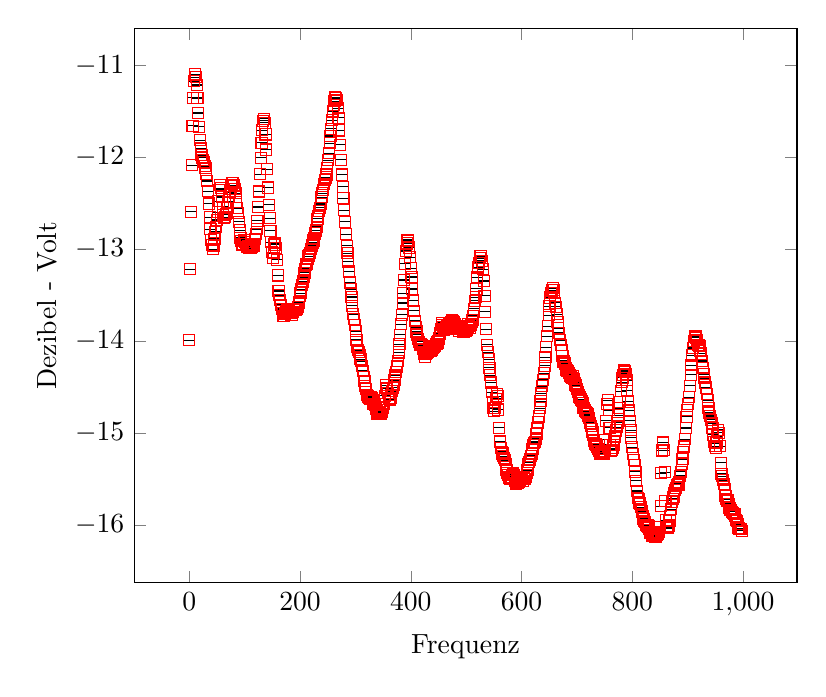
\begin{tikzpicture}
		\pgfplotsset{width=10cm,legend style={font=\footnotesize}}
		\begin{axis}[xlabel={Frequenz},ylabel={Dezibel - Volt},legend cell align=left,legend pos=north west]
		\addplot+[only marks,color=red,mark=square,error bars/.cd,x dir=both,x explicit,y dir=both,y explicit,error bar style={color=black}] table[x=X,y=Y,x error=xerror,y error=yerror,row sep=\\]{
			X	Y	xerror	yerror	\\
			0.0	-13.990863	0	0	\\
			1.464844	-13.220742	0	0	\\
			2.929687	-12.593173	0	0	\\
			4.394531	-12.086301	0	0	\\
			5.859375	-11.659645	0	0	\\
			7.324219	-11.353777	0	0	\\
			8.789062	-11.173666	0	0	\\
			10.253906	-11.099954	0	0	\\
			11.71875	-11.13186	0	0	\\
			13.183594	-11.214862	0	0	\\
			14.648437	-11.356343	0	0	\\
			16.113281	-11.519871	0	0	\\
			17.578125	-11.667393	0	0	\\
			19.042969	-11.815162	0	0	\\
			20.507812	-11.906364	0	0	\\
			21.972656	-11.978109	0	0	\\
			23.4375	-12.003783	0	0	\\
			24.902344	-12.031542	0	0	\\
			26.367187	-12.054852	0	0	\\
			27.832031	-12.097246	0	0	\\
			29.296875	-12.119069	0	0	\\
			30.761719	-12.181365	0	0	\\
			32.226562	-12.258706	0	0	\\
			33.691406	-12.370269	0	0	\\
			35.15625	-12.504201	0	0	\\
			36.621094	-12.655321	0	0	\\
			38.085937	-12.785414	0	0	\\
			39.550781	-12.899312	0	0	\\
			41.015625	-12.958859	0	0	\\
			42.480469	-13.001463	0	0	\\
			43.945312	-12.961015	0	0	\\
			45.410156	-12.887166	0	0	\\
			46.875	-12.813715	0	0	\\
			48.339844	-12.75776	0	0	\\
			49.804687	-12.682851	0	0	\\
			51.269531	-12.597386	0	0	\\
			52.734375	-12.478655	0	0	\\
			54.199219	-12.355413	0	0	\\
			55.664062	-12.30126	0	0	\\
			57.128906	-12.338498	0	0	\\
			58.59375	-12.432709	0	0	\\
			60.058594	-12.540374	0	0	\\
			61.523437	-12.626656	0	0	\\
			62.988281	-12.661065	0	0	\\
			64.453125	-12.654479	0	0	\\
			65.917969	-12.6193	0	0	\\
			67.382812	-12.604296	0	0	\\
			68.847656	-12.551481	0	0	\\
			70.3125	-12.485415	0	0	\\
			71.777344	-12.432659	0	0	\\
			73.242187	-12.381006	0	0	\\
			74.707031	-12.343401	0	0	\\
			76.171875	-12.313676	0	0	\\
			77.636719	-12.286014	0	0	\\
			79.101562	-12.284934	0	0	\\
			80.566406	-12.308036	0	0	\\
			82.03125	-12.345141	0	0	\\
			83.496094	-12.393332	0	0	\\
			84.960937	-12.489784	0	0	\\
			86.425781	-12.555599	0	0	\\
			87.890625	-12.609749	0	0	\\
			89.355469	-12.704456	0	0	\\
			90.820312	-12.794186	0	0	\\
			92.285156	-12.879162	0	0	\\
			93.75	-12.912731	0	0	\\
			95.214844	-12.949125	0	0	\\
			96.679687	-12.940681	0	0	\\
			98.144531	-12.899775	0	0	\\
			99.609375	-12.903327	0	0	\\
			101.074219	-12.91909	0	0	\\
			102.539062	-12.943302	0	0	\\
			104.003906	-12.980621	0	0	\\
			105.46875	-12.976906	0	0	\\
			106.933594	-12.967743	0	0	\\
			108.398437	-12.983293	0	0	\\
			109.863281	-12.989998	0	0	\\
			111.328125	-12.986943	0	0	\\
			112.792969	-12.977329	0	0	\\
			114.257812	-12.963073	0	0	\\
			115.722656	-12.961022	0	0	\\
			117.1875	-12.946528	0	0	\\
			118.652344	-12.890144	0	0	\\
			120.117187	-12.839678	0	0	\\
			121.582031	-12.783311	0	0	\\
			123.046875	-12.691762	0	0	\\
			124.511719	-12.542548	0	0	\\
			125.976562	-12.373331	0	0	\\
			127.441406	-12.18433	0	0	\\
			128.90625	-12.004623	0	0	\\
			130.371094	-11.843703	0	0	\\
			131.835937	-11.707188	0	0	\\
			133.300781	-11.605751	0	0	\\
			134.765625	-11.581333	0	0	\\
			136.230469	-11.625084	0	0	\\
			137.695312	-11.753007	0	0	\\
			139.160156	-11.916752	0	0	\\
			140.625	-12.131978	0	0	\\
			142.089844	-12.330314	0	0	\\
			143.554687	-12.519522	0	0	\\
			145.019531	-12.664799	0	0	\\
			146.484375	-12.800534	0	0	\\
			147.949219	-12.925819	0	0	\\
			149.414062	-13.033598	0	0	\\
			150.878906	-13.098764	0	0	\\
			152.34375	-13.041996	0	0	\\
			153.808594	-12.95048	0	0	\\
			155.273437	-12.934716	0	0	\\
			156.738281	-12.988553	0	0	\\
			158.203125	-13.115672	0	0	\\
			159.667969	-13.286642	0	0	\\
			161.132812	-13.456252	0	0	\\
			162.597656	-13.502826	0	0	\\
			164.0625	-13.553118	0	0	\\
			165.527344	-13.607011	0	0	\\
			166.992187	-13.651397	0	0	\\
			168.457031	-13.691117	0	0	\\
			169.921875	-13.725511	0	0	\\
			171.386719	-13.726735	0	0	\\
			172.851562	-13.710059	0	0	\\
			174.316406	-13.68375	0	0	\\
			175.78125	-13.676395	0	0	\\
			177.246094	-13.666174	0	0	\\
			178.710937	-13.673602	0	0	\\
			180.175781	-13.678099	0	0	\\
			181.640625	-13.691988	0	0	\\
			183.105469	-13.695625	0	0	\\
			184.570312	-13.712811	0	0	\\
			186.035156	-13.720822	0	0	\\
			187.5	-13.684086	0	0	\\
			188.964844	-13.654611	0	0	\\
			190.429687	-13.648312	0	0	\\
			191.894531	-13.662432	0	0	\\
			193.359375	-13.649101	0	0	\\
			194.824219	-13.649775	0	0	\\
			196.289062	-13.62643	0	0	\\
			197.753906	-13.581181	0	0	\\
			199.21875	-13.513991	0	0	\\
			200.683594	-13.479372	0	0	\\
			202.148437	-13.440208	0	0	\\
			203.613281	-13.38937	0	0	\\
			205.078125	-13.352499	0	0	\\
			206.542969	-13.303922	0	0	\\
			208.007812	-13.258434	0	0	\\
			209.472656	-13.214642	0	0	\\
			210.9375	-13.167727	0	0	\\
			212.402344	-13.158678	0	0	\\
			213.867187	-13.106247	0	0	\\
			215.332031	-13.078883	0	0	\\
			216.796875	-13.06086	0	0	\\
			218.261719	-13.043907	0	0	\\
			219.726562	-12.998944	0	0	\\
			221.191406	-12.961837	0	0	\\
			222.65625	-12.932526	0	0	\\
			224.121094	-12.907174	0	0	\\
			225.585937	-12.885682	0	0	\\
			227.050781	-12.829641	0	0	\\
			228.515625	-12.798444	0	0	\\
			229.980469	-12.758844	0	0	\\
			231.445312	-12.67043	0	0	\\
			232.910156	-12.645531	0	0	\\
			234.375	-12.585593	0	0	\\
			235.839844	-12.548909	0	0	\\
			237.304687	-12.509684	0	0	\\
			238.769531	-12.433972	0	0	\\
			240.234375	-12.391083	0	0	\\
			241.699219	-12.352882	0	0	\\
			243.164062	-12.288893	0	0	\\
			244.628906	-12.245725	0	0	\\
			246.09375	-12.220913	0	0	\\
			247.558594	-12.18843	0	0	\\
			249.023437	-12.120901	0	0	\\
			250.488281	-12.033911	0	0	\\
			251.953125	-11.957184	0	0	\\
			253.417969	-11.848174	0	0	\\
			254.882812	-11.770129	0	0	\\
			256.347656	-11.689206	0	0	\\
			257.8125	-11.599123	0	0	\\
			259.277344	-11.502622	0	0	\\
			260.742187	-11.431498	0	0	\\
			262.207031	-11.390035	0	0	\\
			263.671875	-11.351232	0	0	\\
			265.136719	-11.360824	0	0	\\
			266.601562	-11.37674	0	0	\\
			268.066406	-11.468312	0	0	\\
			269.53125	-11.573105	0	0	\\
			270.996094	-11.709112	0	0	\\
			272.460937	-11.864759	0	0	\\
			273.925781	-12.027164	0	0	\\
			275.390625	-12.189106	0	0	\\
			276.855469	-12.321771	0	0	\\
			278.320312	-12.44616	0	0	\\
			279.785156	-12.576815	0	0	\\
			281.25	-12.701351	0	0	\\
			282.714844	-12.838613	0	0	\\
			284.179687	-12.964667	0	0	\\
			285.644531	-13.04579	0	0	\\
			287.109375	-13.135234	0	0	\\
			288.574219	-13.243687	0	0	\\
			290.039062	-13.362682	0	0	\\
			291.503906	-13.434281	0	0	\\
			292.96875	-13.521248	0	0	\\
			294.433594	-13.617717	0	0	\\
			295.898437	-13.710183	0	0	\\
			297.363281	-13.76419	0	0	\\
			298.828125	-13.823544	0	0	\\
			300.292969	-13.895317	0	0	\\
			301.757812	-13.98561	0	0	\\
			303.222656	-14.059311	0	0	\\
			304.6875	-14.098197	0	0	\\
			306.152344	-14.120339	0	0	\\
			307.617187	-14.154343	0	0	\\
			309.082031	-14.196384	0	0	\\
			310.546875	-14.220399	0	0	\\
			312.011719	-14.276128	0	0	\\
			313.476562	-14.323638	0	0	\\
			314.941406	-14.389345	0	0	\\
			316.40625	-14.43097	0	0	\\
			317.871094	-14.491088	0	0	\\
			319.335937	-14.525454	0	0	\\
			320.800781	-14.591373	0	0	\\
			322.265625	-14.603313	0	0	\\
			323.730469	-14.617351	0	0	\\
			325.195312	-14.614722	0	0	\\
			326.660156	-14.633396	0	0	\\
			328.125	-14.607854	0	0	\\
			329.589844	-14.621986	0	0	\\
			331.054687	-14.647774	0	0	\\
			332.519531	-14.689278	0	0	\\
			333.984375	-14.681727	0	0	\\
			335.449219	-14.694976	0	0	\\
			336.914062	-14.733629	0	0	\\
			338.378906	-14.766539	0	0	\\
			339.84375	-14.796078	0	0	\\
			341.308594	-14.778815	0	0	\\
			342.773437	-14.792817	0	0	\\
			344.238281	-14.782312	0	0	\\
			345.703125	-14.789963	0	0	\\
			347.167969	-14.773616	0	0	\\
			348.632812	-14.749795	0	0	\\
			350.097656	-14.732075	0	0	\\
			351.5625	-14.689613	0	0	\\
			353.027344	-14.596697	0	0	\\
			354.492187	-14.510749	0	0	\\
			355.957031	-14.482319	0	0	\\
			357.421875	-14.518177	0	0	\\
			358.886719	-14.565081	0	0	\\
			360.351562	-14.624722	0	0	\\
			361.816406	-14.637166	0	0	\\
			363.28125	-14.622669	0	0	\\
			364.746094	-14.583884	0	0	\\
			366.210937	-14.548106	0	0	\\
			367.675781	-14.509298	0	0	\\
			369.140625	-14.479681	0	0	\\
			370.605469	-14.427382	0	0	\\
			372.070312	-14.375989	0	0	\\
			373.535156	-14.337923	0	0	\\
			375.0	-14.27731	0	0	\\
			376.464844	-14.218415	0	0	\\
			377.929687	-14.124595	0	0	\\
			379.394531	-14.035863	0	0	\\
			380.859375	-13.932402	0	0	\\
			382.324219	-13.816666	0	0	\\
			383.789062	-13.714383	0	0	\\
			385.253906	-13.586818	0	0	\\
			386.71875	-13.478394	0	0	\\
			388.183594	-13.336745	0	0	\\
			389.648437	-13.161298	0	0	\\
			391.113281	-13.020653	0	0	\\
			392.578125	-12.938414	0	0	\\
			394.042969	-12.896828	0	0	\\
			395.507812	-12.908718	0	0	\\
			396.972656	-12.983448	0	0	\\
			398.4375	-13.087122	0	0	\\
			399.902344	-13.206648	0	0	\\
			401.367187	-13.304061	0	0	\\
			402.832031	-13.433686	0	0	\\
			404.296875	-13.55918	0	0	\\
			405.761719	-13.66962	0	0	\\
			407.226562	-13.781556	0	0	\\
			408.691406	-13.849759	0	0	\\
			410.15625	-13.896341	0	0	\\
			411.621094	-13.929201	0	0	\\
			413.085937	-13.978805	0	0	\\
			414.550781	-14.009271	0	0	\\
			416.015625	-14.037761	0	0	\\
			417.480469	-14.032717	0	0	\\
			418.945312	-14.032336	0	0	\\
			420.410156	-14.047141	0	0	\\
			421.875	-14.086824	0	0	\\
			423.339844	-14.116968	0	0	\\
			424.804687	-14.138795	0	0	\\
			426.269531	-14.169562	0	0	\\
			427.734375	-14.145459	0	0	\\
			429.199219	-14.125455	0	0	\\
			430.664062	-14.115338	0	0	\\
			432.128906	-14.109595	0	0	\\
			433.59375	-14.105023	0	0	\\
			435.058594	-14.100994	0	0	\\
			436.523437	-14.105568	0	0	\\
			437.988281	-14.095564	0	0	\\
			439.453125	-14.073872	0	0	\\
			440.917969	-14.067688	0	0	\\
			442.382812	-14.058201	0	0	\\
			443.847656	-14.055595	0	0	\\
			445.3125	-14.031987	0	0	\\
			446.777344	-14.029666	0	0	\\
			448.242187	-14.015606	0	0	\\
			449.707031	-14.00567	0	0	\\
			451.171875	-13.971963	0	0	\\
			452.636719	-13.917448	0	0	\\
			454.101562	-13.871082	0	0	\\
			455.566406	-13.822934	0	0	\\
			457.03125	-13.803292	0	0	\\
			458.496094	-13.84474	0	0	\\
			459.960937	-13.874604	0	0	\\
			461.425781	-13.867284	0	0	\\
			462.890625	-13.853685	0	0	\\
			464.355469	-13.865517	0	0	\\
			465.820312	-13.837238	0	0	\\
			467.285156	-13.837388	0	0	\\
			468.75	-13.812069	0	0	\\
			470.214844	-13.81428	0	0	\\
			471.679687	-13.8031	0	0	\\
			473.144531	-13.792068	0	0	\\
			474.609375	-13.770113	0	0	\\
			476.074219	-13.781504	0	0	\\
			477.539062	-13.794617	0	0	\\
			479.003906	-13.811562	0	0	\\
			480.46875	-13.823158	0	0	\\
			481.933594	-13.837735	0	0	\\
			483.398437	-13.858458	0	0	\\
			484.863281	-13.866255	0	0	\\
			486.328125	-13.894801	0	0	\\
			487.792969	-13.873693	0	0	\\
			489.257812	-13.869926	0	0	\\
			490.722656	-13.867346	0	0	\\
			492.1875	-13.872162	0	0	\\
			493.652344	-13.88931	0	0	\\
			495.117187	-13.897195	0	0	\\
			496.582031	-13.903849	0	0	\\
			498.046875	-13.894648	0	0	\\
			499.511719	-13.889508	0	0	\\
			500.976562	-13.883987	0	0	\\
			502.441406	-13.853021	0	0	\\
			503.90625	-13.816963	0	0	\\
			505.371094	-13.839427	0	0	\\
			506.835937	-13.857006	0	0	\\
			508.300781	-13.82053	0	0	\\
			509.765625	-13.790507	0	0	\\
			511.230469	-13.7723	0	0	\\
			512.695312	-13.724944	0	0	\\
			514.160156	-13.648361	0	0	\\
			515.625	-13.563315	0	0	\\
			517.089844	-13.522591	0	0	\\
			518.554687	-13.432367	0	0	\\
			520.019531	-13.306062	0	0	\\
			521.484375	-13.19997	0	0	\\
			522.949219	-13.14853	0	0	\\
			524.414062	-13.098732	0	0	\\
			525.878906	-13.074825	0	0	\\
			527.34375	-13.073086	0	0	\\
			528.808594	-13.128584	0	0	\\
			530.273437	-13.219419	0	0	\\
			531.738281	-13.34666	0	0	\\
			533.203125	-13.506455	0	0	\\
			534.667969	-13.680025	0	0	\\
			536.132812	-13.872216	0	0	\\
			537.597656	-14.039095	0	0	\\
			539.0625	-14.121045	0	0	\\
			540.527344	-14.197472	0	0	\\
			541.992187	-14.290038	0	0	\\
			543.457031	-14.370574	0	0	\\
			544.921875	-14.451285	0	0	\\
			546.386719	-14.555286	0	0	\\
			547.851562	-14.664212	0	0	\\
			549.316406	-14.728651	0	0	\\
			550.78125	-14.763759	0	0	\\
			552.246094	-14.728044	0	0	\\
			553.710937	-14.630271	0	0	\\
			555.175781	-14.575663	0	0	\\
			556.640625	-14.599288	0	0	\\
			558.105469	-14.745647	0	0	\\
			559.570312	-14.945608	0	0	\\
			561.035156	-15.093082	0	0	\\
			562.5	-15.167777	0	0	\\
			563.964844	-15.205037	0	0	\\
			565.429687	-15.224264	0	0	\\
			566.894531	-15.251722	0	0	\\
			568.359375	-15.274831	0	0	\\
			569.824219	-15.297695	0	0	\\
			571.289062	-15.34111	0	0	\\
			572.753906	-15.400537	0	0	\\
			574.21875	-15.435652	0	0	\\
			575.683594	-15.457136	0	0	\\
			577.148437	-15.485675	0	0	\\
			578.613281	-15.49084	0	0	\\
			580.078125	-15.498753	0	0	\\
			581.542969	-15.504822	0	0	\\
			583.007812	-15.474781	0	0	\\
			584.472656	-15.44119	0	0	\\
			585.9375	-15.459592	0	0	\\
			587.402344	-15.484672	0	0	\\
			588.867187	-15.521551	0	0	\\
			590.332031	-15.550092	0	0	\\
			591.796875	-15.5353	0	0	\\
			593.261719	-15.540442	0	0	\\
			594.726562	-15.534206	0	0	\\
			596.191406	-15.521738	0	0	\\
			597.65625	-15.512017	0	0	\\
			599.121094	-15.496259	0	0	\\
			600.585937	-15.505521	0	0	\\
			602.050781	-15.525478	0	0	\\
			603.515625	-15.489332	0	0	\\
			604.980469	-15.475041	0	0	\\
			606.445312	-15.498472	0	0	\\
			607.910156	-15.4794	0	0	\\
			609.375	-15.440123	0	0	\\
			610.839844	-15.404474	0	0	\\
			612.304687	-15.339426	0	0	\\
			613.769531	-15.319142	0	0	\\
			615.234375	-15.289766	0	0	\\
			616.699219	-15.246541	0	0	\\
			618.164062	-15.224387	0	0	\\
			619.628906	-15.172448	0	0	\\
			621.09375	-15.127989	0	0	\\
			622.558594	-15.11155	0	0	\\
			624.023437	-15.098793	0	0	\\
			625.488281	-15.059893	0	0	\\
			626.953125	-15.014052	0	0	\\
			628.417969	-14.95174	0	0	\\
			629.882812	-14.886176	0	0	\\
			631.347656	-14.820297	0	0	\\
			632.8125	-14.729945	0	0	\\
			634.277344	-14.656614	0	0	\\
			635.742187	-14.570965	0	0	\\
			637.207031	-14.492214	0	0	\\
			638.671875	-14.423053	0	0	\\
			640.136719	-14.349377	0	0	\\
			641.601562	-14.271088	0	0	\\
			643.066406	-14.176852	0	0	\\
			644.53125	-14.06725	0	0	\\
			645.996094	-13.947181	0	0	\\
			647.460937	-13.83753	0	0	\\
			648.925781	-13.721442	0	0	\\
			650.390625	-13.622908	0	0	\\
			651.855469	-13.526862	0	0	\\
			653.320312	-13.477676	0	0	\\
			654.785156	-13.450152	0	0	\\
			656.25	-13.423659	0	0	\\
			657.714844	-13.447421	0	0	\\
			659.179687	-13.475062	0	0	\\
			660.644531	-13.582721	0	0	\\
			662.109375	-13.628484	0	0	\\
			663.574219	-13.707826	0	0	\\
			665.039062	-13.797201	0	0	\\
			666.503906	-13.860761	0	0	\\
			667.96875	-13.912859	0	0	\\
			669.433594	-13.988544	0	0	\\
			670.898437	-14.040359	0	0	\\
			672.363281	-14.101573	0	0	\\
			673.828125	-14.162057	0	0	\\
			675.292969	-14.229001	0	0	\\
			676.757812	-14.216502	0	0	\\
			678.222656	-14.244398	0	0	\\
			679.6875	-14.295232	0	0	\\
			681.152344	-14.317716	0	0	\\
			682.617187	-14.327754	0	0	\\
			684.082031	-14.324483	0	0	\\
			685.546875	-14.349835	0	0	\\
			687.011719	-14.369449	0	0	\\
			688.476562	-14.380431	0	0	\\
			689.941406	-14.394601	0	0	\\
			691.40625	-14.40058	0	0	\\
			692.871094	-14.381015	0	0	\\
			694.335937	-14.409152	0	0	\\
			695.800781	-14.457162	0	0	\\
			697.265625	-14.478003	0	0	\\
			698.730469	-14.491123	0	0	\\
			700.195312	-14.526481	0	0	\\
			701.660156	-14.559084	0	0	\\
			703.125	-14.592401	0	0	\\
			704.589844	-14.611311	0	0	\\
			706.054687	-14.61809	0	0	\\
			707.519531	-14.635436	0	0	\\
			708.984375	-14.655381	0	0	\\
			710.449219	-14.67246	0	0	\\
			711.914062	-14.724585	0	0	\\
			713.378906	-14.729287	0	0	\\
			714.84375	-14.756397	0	0	\\
			716.308594	-14.76883	0	0	\\
			717.773437	-14.780317	0	0	\\
			719.238281	-14.794109	0	0	\\
			720.703125	-14.813333	0	0	\\
			722.167969	-14.834036	0	0	\\
			723.632812	-14.888704	0	0	\\
			725.097656	-14.928528	0	0	\\
			726.5625	-14.961893	0	0	\\
			728.027344	-14.988379	0	0	\\
			729.492187	-15.019583	0	0	\\
			730.957031	-15.082822	0	0	\\
			732.421875	-15.117656	0	0	\\
			733.886719	-15.119081	0	0	\\
			735.351562	-15.128799	0	0	\\
			736.816406	-15.152591	0	0	\\
			738.28125	-15.177332	0	0	\\
			739.746094	-15.19936	0	0	\\
			741.210937	-15.225313	0	0	\\
			742.675781	-15.228173	0	0	\\
			744.140625	-15.215064	0	0	\\
			745.605469	-15.202934	0	0	\\
			747.070312	-15.230885	0	0	\\
			748.535156	-15.22381	0	0	\\
			750.0	-15.198152	0	0	\\
			751.464844	-15.076041	0	0	\\
			752.929687	-14.867378	0	0	\\
			754.394531	-14.687699	0	0	\\
			755.859375	-14.645307	0	0	\\
			757.324219	-14.753813	0	0	\\
			758.789062	-14.942417	0	0	\\
			760.253906	-15.131748	0	0	\\
			761.71875	-15.195743	0	0	\\
			763.183594	-15.181857	0	0	\\
			764.648437	-15.167159	0	0	\\
			766.113281	-15.135545	0	0	\\
			767.578125	-15.088744	0	0	\\
			769.042969	-15.038885	0	0	\\
			770.507812	-14.972694	0	0	\\
			771.972656	-14.937998	0	0	\\
			773.4375	-14.890587	0	0	\\
			774.902344	-14.809068	0	0	\\
			776.367187	-14.730096	0	0	\\
			777.832031	-14.667745	0	0	\\
			779.296875	-14.547952	0	0	\\
			780.761719	-14.44797	0	0	\\
			782.226562	-14.400951	0	0	\\
			783.691406	-14.366796	0	0	\\
			785.15625	-14.32078	0	0	\\
			786.621094	-14.331855	0	0	\\
			788.085937	-14.359122	0	0	\\
			789.550781	-14.427865	0	0	\\
			791.015625	-14.54172	0	0	\\
			792.480469	-14.658217	0	0	\\
			793.945312	-14.75583	0	0	\\
			795.410156	-14.868972	0	0	\\
			796.875	-14.969853	0	0	\\
			798.339844	-15.051834	0	0	\\
			799.804687	-15.154334	0	0	\\
			801.269531	-15.233349	0	0	\\
			802.734375	-15.292773	0	0	\\
			804.199219	-15.352299	0	0	\\
			805.664062	-15.42327	0	0	\\
			807.128906	-15.518469	0	0	\\
			808.59375	-15.631898	0	0	\\
			810.058594	-15.703532	0	0	\\
			811.523437	-15.714788	0	0	\\
			812.988281	-15.764438	0	0	\\
			814.453125	-15.770402	0	0	\\
			815.917969	-15.809488	0	0	\\
			817.382812	-15.853879	0	0	\\
			818.847656	-15.904475	0	0	\\
			820.3125	-15.934531	0	0	\\
			821.777344	-15.959701	0	0	\\
			823.242187	-15.968832	0	0	\\
			824.707031	-16.004521	0	0	\\
			826.171875	-16.011148	0	0	\\
			827.636719	-15.997603	0	0	\\
			829.101562	-16.017642	0	0	\\
			830.566406	-16.038706	0	0	\\
			832.03125	-16.089245	0	0	\\
			833.496094	-16.080362	0	0	\\
			834.960937	-16.100063	0	0	\\
			836.425781	-16.116341	0	0	\\
			837.890625	-16.113755	0	0	\\
			839.355469	-16.120453	0	0	\\
			840.820312	-16.126907	0	0	\\
			842.285156	-16.127852	0	0	\\
			843.75	-16.110194	0	0	\\
			845.214844	-16.090892	0	0	\\
			846.679687	-16.095004	0	0	\\
			848.144531	-16.076038	0	0	\\
			849.609375	-16.028352	0	0	\\
			851.074219	-15.799283	0	0	\\
			852.539062	-15.436943	0	0	\\
			854.003906	-15.191048	0	0	\\
			855.46875	-15.104776	0	0	\\
			856.933594	-15.186292	0	0	\\
			858.398437	-15.428185	0	0	\\
			859.863281	-15.739545	0	0	\\
			861.328125	-15.950102	0	0	\\
			862.792969	-16.025449	0	0	\\
			864.257812	-16.03453	0	0	\\
			865.722656	-16.007516	0	0	\\
			867.1875	-15.961047	0	0	\\
			868.652344	-15.902111	0	0	\\
			870.117187	-15.829222	0	0	\\
			871.582031	-15.754673	0	0	\\
			873.046875	-15.716194	0	0	\\
			874.511719	-15.694562	0	0	\\
			875.976562	-15.659212	0	0	\\
			877.441406	-15.621526	0	0	\\
			878.90625	-15.599733	0	0	\\
			880.371094	-15.565716	0	0	\\
			881.835937	-15.551222	0	0	\\
			883.300781	-15.562498	0	0	\\
			884.765625	-15.532753	0	0	\\
			886.230469	-15.467556	0	0	\\
			887.695312	-15.421785	0	0	\\
			889.160156	-15.341757	0	0	\\
			890.625	-15.283292	0	0	\\
			892.089844	-15.207176	0	0	\\
			893.554687	-15.14761	0	0	\\
			895.019531	-15.070186	0	0	\\
			896.484375	-14.946816	0	0	\\
			897.949219	-14.823093	0	0	\\
			899.414062	-14.749311	0	0	\\
			900.878906	-14.686024	0	0	\\
			902.34375	-14.610228	0	0	\\
			903.808594	-14.487092	0	0	\\
			905.273437	-14.365865	0	0	\\
			906.738281	-14.265327	0	0	\\
			908.203125	-14.156753	0	0	\\
			909.667969	-14.075426	0	0	\\
			911.132812	-14.000932	0	0	\\
			912.597656	-13.956787	0	0	\\
			914.0625	-13.943982	0	0	\\
			915.527344	-13.962732	0	0	\\
			916.992187	-13.991856	0	0	\\
			918.457031	-14.043238	0	0	\\
			919.921875	-14.039422	0	0	\\
			921.386719	-14.052556	0	0	\\
			922.851562	-14.103051	0	0	\\
			924.316406	-14.136733	0	0	\\
			925.78125	-14.216822	0	0	\\
			927.246094	-14.295622	0	0	\\
			928.710937	-14.361802	0	0	\\
			930.175781	-14.403763	0	0	\\
			931.640625	-14.45205	0	0	\\
			933.105469	-14.506171	0	0	\\
			934.570312	-14.572555	0	0	\\
			936.035156	-14.646006	0	0	\\
			937.5	-14.725074	0	0	\\
			938.964844	-14.777822	0	0	\\
			940.429687	-14.816002	0	0	\\
			941.894531	-14.856926	0	0	\\
			943.359375	-14.897443	0	0	\\
			944.824219	-14.949587	0	0	\\
			946.289062	-15.017854	0	0	\\
			947.753906	-15.095573	0	0	\\
			949.21875	-15.146074	0	0	\\
			950.683594	-15.159279	0	0	\\
			952.148437	-15.108893	0	0	\\
			953.613281	-15.037326	0	0	\\
			955.078125	-14.965295	0	0	\\
			956.542969	-14.999358	0	0	\\
			958.007812	-15.144328	0	0	\\
			959.472656	-15.325438	0	0	\\
			960.9375	-15.445549	0	0	\\
			962.402344	-15.469093	0	0	\\
			963.867187	-15.514895	0	0	\\
			965.332031	-15.554472	0	0	\\
			966.796875	-15.615324	0	0	\\
			968.261719	-15.684311	0	0	\\
			969.726562	-15.71788	0	0	\\
			971.191406	-15.74427	0	0	\\
			972.65625	-15.725927	0	0	\\
			974.121094	-15.769095	0	0	\\
			975.585937	-15.816503	0	0	\\
			977.050781	-15.83649	0	0	\\
			978.515625	-15.842746	0	0	\\
			979.980469	-15.855846	0	0	\\
			981.445312	-15.873752	0	0	\\
			982.910156	-15.881763	0	0	\\
			984.375	-15.879912	0	0	\\
			985.839844	-15.898695	0	0	\\
			987.304687	-15.94639	0	0	\\
			988.769531	-15.96004	0	0	\\
			990.234375	-15.990263	0	0	\\
			991.699219	-16.037982	0	0	\\
			993.164062	-16.044649	0	0	\\
			994.628906	-16.048308	0	0	\\
			996.09375	-16.045975	0	0	\\
			997.558594	-16.06603	0	0	\\
		};		% \addlegendentry{Messpunkte Datensatz 0}
		\end{axis}
		\end{tikzpicture}
	\caption{Umgebung}
	\label{fig:Umgebungsmessung}
\end{figure}
            \begin{figure}[H]
	\centering
	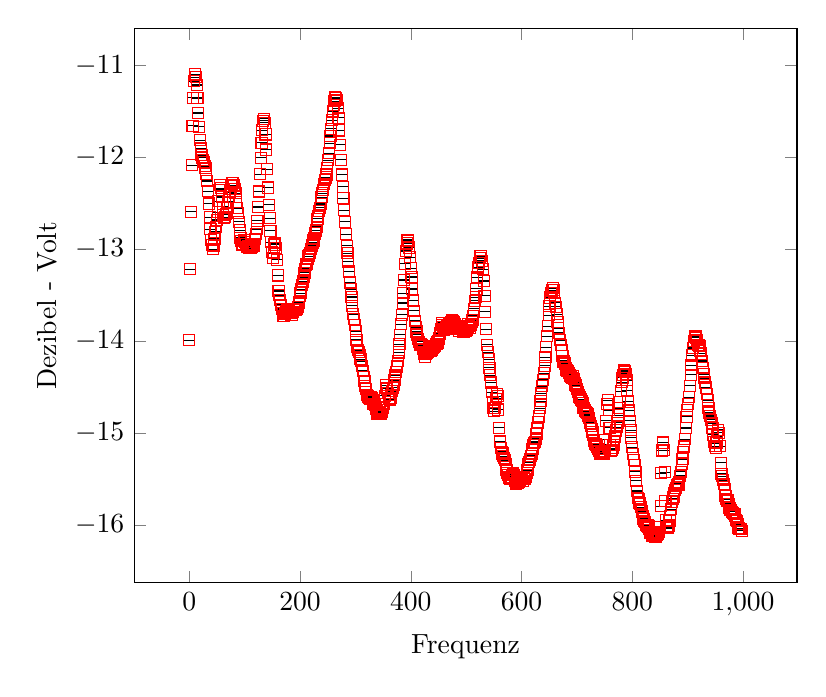
\begin{tikzpicture}
		\pgfplotsset{width=10cm,legend style={font=\footnotesize}}
		\begin{axis}[xlabel={Frequenz},ylabel={Dezibel - Volt},legend cell align=left,legend pos=north west]
		\addplot+[only marks,color=red,mark=square,error bars/.cd,x dir=both,x explicit,y dir=both,y explicit,error bar style={color=black}] table[x=X,y=Y,x error=xerror,y error=yerror,row sep=\\]{
			X	Y	xerror	yerror	\\
			0.0	-13.990863	0	0	\\
			1.464844	-13.220742	0	0	\\
			2.929687	-12.593173	0	0	\\
			4.394531	-12.086301	0	0	\\
			5.859375	-11.659645	0	0	\\
			7.324219	-11.353777	0	0	\\
			8.789062	-11.173666	0	0	\\
			10.253906	-11.099954	0	0	\\
			11.71875	-11.13186	0	0	\\
			13.183594	-11.214862	0	0	\\
			14.648437	-11.356343	0	0	\\
			16.113281	-11.519871	0	0	\\
			17.578125	-11.667393	0	0	\\
			19.042969	-11.815162	0	0	\\
			20.507812	-11.906364	0	0	\\
			21.972656	-11.978109	0	0	\\
			23.4375	-12.003783	0	0	\\
			24.902344	-12.031542	0	0	\\
			26.367187	-12.054852	0	0	\\
			27.832031	-12.097246	0	0	\\
			29.296875	-12.119069	0	0	\\
			30.761719	-12.181365	0	0	\\
			32.226562	-12.258706	0	0	\\
			33.691406	-12.370269	0	0	\\
			35.15625	-12.504201	0	0	\\
			36.621094	-12.655321	0	0	\\
			38.085937	-12.785414	0	0	\\
			39.550781	-12.899312	0	0	\\
			41.015625	-12.958859	0	0	\\
			42.480469	-13.001463	0	0	\\
			43.945312	-12.961015	0	0	\\
			45.410156	-12.887166	0	0	\\
			46.875	-12.813715	0	0	\\
			48.339844	-12.75776	0	0	\\
			49.804687	-12.682851	0	0	\\
			51.269531	-12.597386	0	0	\\
			52.734375	-12.478655	0	0	\\
			54.199219	-12.355413	0	0	\\
			55.664062	-12.30126	0	0	\\
			57.128906	-12.338498	0	0	\\
			58.59375	-12.432709	0	0	\\
			60.058594	-12.540374	0	0	\\
			61.523437	-12.626656	0	0	\\
			62.988281	-12.661065	0	0	\\
			64.453125	-12.654479	0	0	\\
			65.917969	-12.6193	0	0	\\
			67.382812	-12.604296	0	0	\\
			68.847656	-12.551481	0	0	\\
			70.3125	-12.485415	0	0	\\
			71.777344	-12.432659	0	0	\\
			73.242187	-12.381006	0	0	\\
			74.707031	-12.343401	0	0	\\
			76.171875	-12.313676	0	0	\\
			77.636719	-12.286014	0	0	\\
			79.101562	-12.284934	0	0	\\
			80.566406	-12.308036	0	0	\\
			82.03125	-12.345141	0	0	\\
			83.496094	-12.393332	0	0	\\
			84.960937	-12.489784	0	0	\\
			86.425781	-12.555599	0	0	\\
			87.890625	-12.609749	0	0	\\
			89.355469	-12.704456	0	0	\\
			90.820312	-12.794186	0	0	\\
			92.285156	-12.879162	0	0	\\
			93.75	-12.912731	0	0	\\
			95.214844	-12.949125	0	0	\\
			96.679687	-12.940681	0	0	\\
			98.144531	-12.899775	0	0	\\
			99.609375	-12.903327	0	0	\\
			101.074219	-12.91909	0	0	\\
			102.539062	-12.943302	0	0	\\
			104.003906	-12.980621	0	0	\\
			105.46875	-12.976906	0	0	\\
			106.933594	-12.967743	0	0	\\
			108.398437	-12.983293	0	0	\\
			109.863281	-12.989998	0	0	\\
			111.328125	-12.986943	0	0	\\
			112.792969	-12.977329	0	0	\\
			114.257812	-12.963073	0	0	\\
			115.722656	-12.961022	0	0	\\
			117.1875	-12.946528	0	0	\\
			118.652344	-12.890144	0	0	\\
			120.117187	-12.839678	0	0	\\
			121.582031	-12.783311	0	0	\\
			123.046875	-12.691762	0	0	\\
			124.511719	-12.542548	0	0	\\
			125.976562	-12.373331	0	0	\\
			127.441406	-12.18433	0	0	\\
			128.90625	-12.004623	0	0	\\
			130.371094	-11.843703	0	0	\\
			131.835937	-11.707188	0	0	\\
			133.300781	-11.605751	0	0	\\
			134.765625	-11.581333	0	0	\\
			136.230469	-11.625084	0	0	\\
			137.695312	-11.753007	0	0	\\
			139.160156	-11.916752	0	0	\\
			140.625	-12.131978	0	0	\\
			142.089844	-12.330314	0	0	\\
			143.554687	-12.519522	0	0	\\
			145.019531	-12.664799	0	0	\\
			146.484375	-12.800534	0	0	\\
			147.949219	-12.925819	0	0	\\
			149.414062	-13.033598	0	0	\\
			150.878906	-13.098764	0	0	\\
			152.34375	-13.041996	0	0	\\
			153.808594	-12.95048	0	0	\\
			155.273437	-12.934716	0	0	\\
			156.738281	-12.988553	0	0	\\
			158.203125	-13.115672	0	0	\\
			159.667969	-13.286642	0	0	\\
			161.132812	-13.456252	0	0	\\
			162.597656	-13.502826	0	0	\\
			164.0625	-13.553118	0	0	\\
			165.527344	-13.607011	0	0	\\
			166.992187	-13.651397	0	0	\\
			168.457031	-13.691117	0	0	\\
			169.921875	-13.725511	0	0	\\
			171.386719	-13.726735	0	0	\\
			172.851562	-13.710059	0	0	\\
			174.316406	-13.68375	0	0	\\
			175.78125	-13.676395	0	0	\\
			177.246094	-13.666174	0	0	\\
			178.710937	-13.673602	0	0	\\
			180.175781	-13.678099	0	0	\\
			181.640625	-13.691988	0	0	\\
			183.105469	-13.695625	0	0	\\
			184.570312	-13.712811	0	0	\\
			186.035156	-13.720822	0	0	\\
			187.5	-13.684086	0	0	\\
			188.964844	-13.654611	0	0	\\
			190.429687	-13.648312	0	0	\\
			191.894531	-13.662432	0	0	\\
			193.359375	-13.649101	0	0	\\
			194.824219	-13.649775	0	0	\\
			196.289062	-13.62643	0	0	\\
			197.753906	-13.581181	0	0	\\
			199.21875	-13.513991	0	0	\\
			200.683594	-13.479372	0	0	\\
			202.148437	-13.440208	0	0	\\
			203.613281	-13.38937	0	0	\\
			205.078125	-13.352499	0	0	\\
			206.542969	-13.303922	0	0	\\
			208.007812	-13.258434	0	0	\\
			209.472656	-13.214642	0	0	\\
			210.9375	-13.167727	0	0	\\
			212.402344	-13.158678	0	0	\\
			213.867187	-13.106247	0	0	\\
			215.332031	-13.078883	0	0	\\
			216.796875	-13.06086	0	0	\\
			218.261719	-13.043907	0	0	\\
			219.726562	-12.998944	0	0	\\
			221.191406	-12.961837	0	0	\\
			222.65625	-12.932526	0	0	\\
			224.121094	-12.907174	0	0	\\
			225.585937	-12.885682	0	0	\\
			227.050781	-12.829641	0	0	\\
			228.515625	-12.798444	0	0	\\
			229.980469	-12.758844	0	0	\\
			231.445312	-12.67043	0	0	\\
			232.910156	-12.645531	0	0	\\
			234.375	-12.585593	0	0	\\
			235.839844	-12.548909	0	0	\\
			237.304687	-12.509684	0	0	\\
			238.769531	-12.433972	0	0	\\
			240.234375	-12.391083	0	0	\\
			241.699219	-12.352882	0	0	\\
			243.164062	-12.288893	0	0	\\
			244.628906	-12.245725	0	0	\\
			246.09375	-12.220913	0	0	\\
			247.558594	-12.18843	0	0	\\
			249.023437	-12.120901	0	0	\\
			250.488281	-12.033911	0	0	\\
			251.953125	-11.957184	0	0	\\
			253.417969	-11.848174	0	0	\\
			254.882812	-11.770129	0	0	\\
			256.347656	-11.689206	0	0	\\
			257.8125	-11.599123	0	0	\\
			259.277344	-11.502622	0	0	\\
			260.742187	-11.431498	0	0	\\
			262.207031	-11.390035	0	0	\\
			263.671875	-11.351232	0	0	\\
			265.136719	-11.360824	0	0	\\
			266.601562	-11.37674	0	0	\\
			268.066406	-11.468312	0	0	\\
			269.53125	-11.573105	0	0	\\
			270.996094	-11.709112	0	0	\\
			272.460937	-11.864759	0	0	\\
			273.925781	-12.027164	0	0	\\
			275.390625	-12.189106	0	0	\\
			276.855469	-12.321771	0	0	\\
			278.320312	-12.44616	0	0	\\
			279.785156	-12.576815	0	0	\\
			281.25	-12.701351	0	0	\\
			282.714844	-12.838613	0	0	\\
			284.179687	-12.964667	0	0	\\
			285.644531	-13.04579	0	0	\\
			287.109375	-13.135234	0	0	\\
			288.574219	-13.243687	0	0	\\
			290.039062	-13.362682	0	0	\\
			291.503906	-13.434281	0	0	\\
			292.96875	-13.521248	0	0	\\
			294.433594	-13.617717	0	0	\\
			295.898437	-13.710183	0	0	\\
			297.363281	-13.76419	0	0	\\
			298.828125	-13.823544	0	0	\\
			300.292969	-13.895317	0	0	\\
			301.757812	-13.98561	0	0	\\
			303.222656	-14.059311	0	0	\\
			304.6875	-14.098197	0	0	\\
			306.152344	-14.120339	0	0	\\
			307.617187	-14.154343	0	0	\\
			309.082031	-14.196384	0	0	\\
			310.546875	-14.220399	0	0	\\
			312.011719	-14.276128	0	0	\\
			313.476562	-14.323638	0	0	\\
			314.941406	-14.389345	0	0	\\
			316.40625	-14.43097	0	0	\\
			317.871094	-14.491088	0	0	\\
			319.335937	-14.525454	0	0	\\
			320.800781	-14.591373	0	0	\\
			322.265625	-14.603313	0	0	\\
			323.730469	-14.617351	0	0	\\
			325.195312	-14.614722	0	0	\\
			326.660156	-14.633396	0	0	\\
			328.125	-14.607854	0	0	\\
			329.589844	-14.621986	0	0	\\
			331.054687	-14.647774	0	0	\\
			332.519531	-14.689278	0	0	\\
			333.984375	-14.681727	0	0	\\
			335.449219	-14.694976	0	0	\\
			336.914062	-14.733629	0	0	\\
			338.378906	-14.766539	0	0	\\
			339.84375	-14.796078	0	0	\\
			341.308594	-14.778815	0	0	\\
			342.773437	-14.792817	0	0	\\
			344.238281	-14.782312	0	0	\\
			345.703125	-14.789963	0	0	\\
			347.167969	-14.773616	0	0	\\
			348.632812	-14.749795	0	0	\\
			350.097656	-14.732075	0	0	\\
			351.5625	-14.689613	0	0	\\
			353.027344	-14.596697	0	0	\\
			354.492187	-14.510749	0	0	\\
			355.957031	-14.482319	0	0	\\
			357.421875	-14.518177	0	0	\\
			358.886719	-14.565081	0	0	\\
			360.351562	-14.624722	0	0	\\
			361.816406	-14.637166	0	0	\\
			363.28125	-14.622669	0	0	\\
			364.746094	-14.583884	0	0	\\
			366.210937	-14.548106	0	0	\\
			367.675781	-14.509298	0	0	\\
			369.140625	-14.479681	0	0	\\
			370.605469	-14.427382	0	0	\\
			372.070312	-14.375989	0	0	\\
			373.535156	-14.337923	0	0	\\
			375.0	-14.27731	0	0	\\
			376.464844	-14.218415	0	0	\\
			377.929687	-14.124595	0	0	\\
			379.394531	-14.035863	0	0	\\
			380.859375	-13.932402	0	0	\\
			382.324219	-13.816666	0	0	\\
			383.789062	-13.714383	0	0	\\
			385.253906	-13.586818	0	0	\\
			386.71875	-13.478394	0	0	\\
			388.183594	-13.336745	0	0	\\
			389.648437	-13.161298	0	0	\\
			391.113281	-13.020653	0	0	\\
			392.578125	-12.938414	0	0	\\
			394.042969	-12.896828	0	0	\\
			395.507812	-12.908718	0	0	\\
			396.972656	-12.983448	0	0	\\
			398.4375	-13.087122	0	0	\\
			399.902344	-13.206648	0	0	\\
			401.367187	-13.304061	0	0	\\
			402.832031	-13.433686	0	0	\\
			404.296875	-13.55918	0	0	\\
			405.761719	-13.66962	0	0	\\
			407.226562	-13.781556	0	0	\\
			408.691406	-13.849759	0	0	\\
			410.15625	-13.896341	0	0	\\
			411.621094	-13.929201	0	0	\\
			413.085937	-13.978805	0	0	\\
			414.550781	-14.009271	0	0	\\
			416.015625	-14.037761	0	0	\\
			417.480469	-14.032717	0	0	\\
			418.945312	-14.032336	0	0	\\
			420.410156	-14.047141	0	0	\\
			421.875	-14.086824	0	0	\\
			423.339844	-14.116968	0	0	\\
			424.804687	-14.138795	0	0	\\
			426.269531	-14.169562	0	0	\\
			427.734375	-14.145459	0	0	\\
			429.199219	-14.125455	0	0	\\
			430.664062	-14.115338	0	0	\\
			432.128906	-14.109595	0	0	\\
			433.59375	-14.105023	0	0	\\
			435.058594	-14.100994	0	0	\\
			436.523437	-14.105568	0	0	\\
			437.988281	-14.095564	0	0	\\
			439.453125	-14.073872	0	0	\\
			440.917969	-14.067688	0	0	\\
			442.382812	-14.058201	0	0	\\
			443.847656	-14.055595	0	0	\\
			445.3125	-14.031987	0	0	\\
			446.777344	-14.029666	0	0	\\
			448.242187	-14.015606	0	0	\\
			449.707031	-14.00567	0	0	\\
			451.171875	-13.971963	0	0	\\
			452.636719	-13.917448	0	0	\\
			454.101562	-13.871082	0	0	\\
			455.566406	-13.822934	0	0	\\
			457.03125	-13.803292	0	0	\\
			458.496094	-13.84474	0	0	\\
			459.960937	-13.874604	0	0	\\
			461.425781	-13.867284	0	0	\\
			462.890625	-13.853685	0	0	\\
			464.355469	-13.865517	0	0	\\
			465.820312	-13.837238	0	0	\\
			467.285156	-13.837388	0	0	\\
			468.75	-13.812069	0	0	\\
			470.214844	-13.81428	0	0	\\
			471.679687	-13.8031	0	0	\\
			473.144531	-13.792068	0	0	\\
			474.609375	-13.770113	0	0	\\
			476.074219	-13.781504	0	0	\\
			477.539062	-13.794617	0	0	\\
			479.003906	-13.811562	0	0	\\
			480.46875	-13.823158	0	0	\\
			481.933594	-13.837735	0	0	\\
			483.398437	-13.858458	0	0	\\
			484.863281	-13.866255	0	0	\\
			486.328125	-13.894801	0	0	\\
			487.792969	-13.873693	0	0	\\
			489.257812	-13.869926	0	0	\\
			490.722656	-13.867346	0	0	\\
			492.1875	-13.872162	0	0	\\
			493.652344	-13.88931	0	0	\\
			495.117187	-13.897195	0	0	\\
			496.582031	-13.903849	0	0	\\
			498.046875	-13.894648	0	0	\\
			499.511719	-13.889508	0	0	\\
			500.976562	-13.883987	0	0	\\
			502.441406	-13.853021	0	0	\\
			503.90625	-13.816963	0	0	\\
			505.371094	-13.839427	0	0	\\
			506.835937	-13.857006	0	0	\\
			508.300781	-13.82053	0	0	\\
			509.765625	-13.790507	0	0	\\
			511.230469	-13.7723	0	0	\\
			512.695312	-13.724944	0	0	\\
			514.160156	-13.648361	0	0	\\
			515.625	-13.563315	0	0	\\
			517.089844	-13.522591	0	0	\\
			518.554687	-13.432367	0	0	\\
			520.019531	-13.306062	0	0	\\
			521.484375	-13.19997	0	0	\\
			522.949219	-13.14853	0	0	\\
			524.414062	-13.098732	0	0	\\
			525.878906	-13.074825	0	0	\\
			527.34375	-13.073086	0	0	\\
			528.808594	-13.128584	0	0	\\
			530.273437	-13.219419	0	0	\\
			531.738281	-13.34666	0	0	\\
			533.203125	-13.506455	0	0	\\
			534.667969	-13.680025	0	0	\\
			536.132812	-13.872216	0	0	\\
			537.597656	-14.039095	0	0	\\
			539.0625	-14.121045	0	0	\\
			540.527344	-14.197472	0	0	\\
			541.992187	-14.290038	0	0	\\
			543.457031	-14.370574	0	0	\\
			544.921875	-14.451285	0	0	\\
			546.386719	-14.555286	0	0	\\
			547.851562	-14.664212	0	0	\\
			549.316406	-14.728651	0	0	\\
			550.78125	-14.763759	0	0	\\
			552.246094	-14.728044	0	0	\\
			553.710937	-14.630271	0	0	\\
			555.175781	-14.575663	0	0	\\
			556.640625	-14.599288	0	0	\\
			558.105469	-14.745647	0	0	\\
			559.570312	-14.945608	0	0	\\
			561.035156	-15.093082	0	0	\\
			562.5	-15.167777	0	0	\\
			563.964844	-15.205037	0	0	\\
			565.429687	-15.224264	0	0	\\
			566.894531	-15.251722	0	0	\\
			568.359375	-15.274831	0	0	\\
			569.824219	-15.297695	0	0	\\
			571.289062	-15.34111	0	0	\\
			572.753906	-15.400537	0	0	\\
			574.21875	-15.435652	0	0	\\
			575.683594	-15.457136	0	0	\\
			577.148437	-15.485675	0	0	\\
			578.613281	-15.49084	0	0	\\
			580.078125	-15.498753	0	0	\\
			581.542969	-15.504822	0	0	\\
			583.007812	-15.474781	0	0	\\
			584.472656	-15.44119	0	0	\\
			585.9375	-15.459592	0	0	\\
			587.402344	-15.484672	0	0	\\
			588.867187	-15.521551	0	0	\\
			590.332031	-15.550092	0	0	\\
			591.796875	-15.5353	0	0	\\
			593.261719	-15.540442	0	0	\\
			594.726562	-15.534206	0	0	\\
			596.191406	-15.521738	0	0	\\
			597.65625	-15.512017	0	0	\\
			599.121094	-15.496259	0	0	\\
			600.585937	-15.505521	0	0	\\
			602.050781	-15.525478	0	0	\\
			603.515625	-15.489332	0	0	\\
			604.980469	-15.475041	0	0	\\
			606.445312	-15.498472	0	0	\\
			607.910156	-15.4794	0	0	\\
			609.375	-15.440123	0	0	\\
			610.839844	-15.404474	0	0	\\
			612.304687	-15.339426	0	0	\\
			613.769531	-15.319142	0	0	\\
			615.234375	-15.289766	0	0	\\
			616.699219	-15.246541	0	0	\\
			618.164062	-15.224387	0	0	\\
			619.628906	-15.172448	0	0	\\
			621.09375	-15.127989	0	0	\\
			622.558594	-15.11155	0	0	\\
			624.023437	-15.098793	0	0	\\
			625.488281	-15.059893	0	0	\\
			626.953125	-15.014052	0	0	\\
			628.417969	-14.95174	0	0	\\
			629.882812	-14.886176	0	0	\\
			631.347656	-14.820297	0	0	\\
			632.8125	-14.729945	0	0	\\
			634.277344	-14.656614	0	0	\\
			635.742187	-14.570965	0	0	\\
			637.207031	-14.492214	0	0	\\
			638.671875	-14.423053	0	0	\\
			640.136719	-14.349377	0	0	\\
			641.601562	-14.271088	0	0	\\
			643.066406	-14.176852	0	0	\\
			644.53125	-14.06725	0	0	\\
			645.996094	-13.947181	0	0	\\
			647.460937	-13.83753	0	0	\\
			648.925781	-13.721442	0	0	\\
			650.390625	-13.622908	0	0	\\
			651.855469	-13.526862	0	0	\\
			653.320312	-13.477676	0	0	\\
			654.785156	-13.450152	0	0	\\
			656.25	-13.423659	0	0	\\
			657.714844	-13.447421	0	0	\\
			659.179687	-13.475062	0	0	\\
			660.644531	-13.582721	0	0	\\
			662.109375	-13.628484	0	0	\\
			663.574219	-13.707826	0	0	\\
			665.039062	-13.797201	0	0	\\
			666.503906	-13.860761	0	0	\\
			667.96875	-13.912859	0	0	\\
			669.433594	-13.988544	0	0	\\
			670.898437	-14.040359	0	0	\\
			672.363281	-14.101573	0	0	\\
			673.828125	-14.162057	0	0	\\
			675.292969	-14.229001	0	0	\\
			676.757812	-14.216502	0	0	\\
			678.222656	-14.244398	0	0	\\
			679.6875	-14.295232	0	0	\\
			681.152344	-14.317716	0	0	\\
			682.617187	-14.327754	0	0	\\
			684.082031	-14.324483	0	0	\\
			685.546875	-14.349835	0	0	\\
			687.011719	-14.369449	0	0	\\
			688.476562	-14.380431	0	0	\\
			689.941406	-14.394601	0	0	\\
			691.40625	-14.40058	0	0	\\
			692.871094	-14.381015	0	0	\\
			694.335937	-14.409152	0	0	\\
			695.800781	-14.457162	0	0	\\
			697.265625	-14.478003	0	0	\\
			698.730469	-14.491123	0	0	\\
			700.195312	-14.526481	0	0	\\
			701.660156	-14.559084	0	0	\\
			703.125	-14.592401	0	0	\\
			704.589844	-14.611311	0	0	\\
			706.054687	-14.61809	0	0	\\
			707.519531	-14.635436	0	0	\\
			708.984375	-14.655381	0	0	\\
			710.449219	-14.67246	0	0	\\
			711.914062	-14.724585	0	0	\\
			713.378906	-14.729287	0	0	\\
			714.84375	-14.756397	0	0	\\
			716.308594	-14.76883	0	0	\\
			717.773437	-14.780317	0	0	\\
			719.238281	-14.794109	0	0	\\
			720.703125	-14.813333	0	0	\\
			722.167969	-14.834036	0	0	\\
			723.632812	-14.888704	0	0	\\
			725.097656	-14.928528	0	0	\\
			726.5625	-14.961893	0	0	\\
			728.027344	-14.988379	0	0	\\
			729.492187	-15.019583	0	0	\\
			730.957031	-15.082822	0	0	\\
			732.421875	-15.117656	0	0	\\
			733.886719	-15.119081	0	0	\\
			735.351562	-15.128799	0	0	\\
			736.816406	-15.152591	0	0	\\
			738.28125	-15.177332	0	0	\\
			739.746094	-15.19936	0	0	\\
			741.210937	-15.225313	0	0	\\
			742.675781	-15.228173	0	0	\\
			744.140625	-15.215064	0	0	\\
			745.605469	-15.202934	0	0	\\
			747.070312	-15.230885	0	0	\\
			748.535156	-15.22381	0	0	\\
			750.0	-15.198152	0	0	\\
			751.464844	-15.076041	0	0	\\
			752.929687	-14.867378	0	0	\\
			754.394531	-14.687699	0	0	\\
			755.859375	-14.645307	0	0	\\
			757.324219	-14.753813	0	0	\\
			758.789062	-14.942417	0	0	\\
			760.253906	-15.131748	0	0	\\
			761.71875	-15.195743	0	0	\\
			763.183594	-15.181857	0	0	\\
			764.648437	-15.167159	0	0	\\
			766.113281	-15.135545	0	0	\\
			767.578125	-15.088744	0	0	\\
			769.042969	-15.038885	0	0	\\
			770.507812	-14.972694	0	0	\\
			771.972656	-14.937998	0	0	\\
			773.4375	-14.890587	0	0	\\
			774.902344	-14.809068	0	0	\\
			776.367187	-14.730096	0	0	\\
			777.832031	-14.667745	0	0	\\
			779.296875	-14.547952	0	0	\\
			780.761719	-14.44797	0	0	\\
			782.226562	-14.400951	0	0	\\
			783.691406	-14.366796	0	0	\\
			785.15625	-14.32078	0	0	\\
			786.621094	-14.331855	0	0	\\
			788.085937	-14.359122	0	0	\\
			789.550781	-14.427865	0	0	\\
			791.015625	-14.54172	0	0	\\
			792.480469	-14.658217	0	0	\\
			793.945312	-14.75583	0	0	\\
			795.410156	-14.868972	0	0	\\
			796.875	-14.969853	0	0	\\
			798.339844	-15.051834	0	0	\\
			799.804687	-15.154334	0	0	\\
			801.269531	-15.233349	0	0	\\
			802.734375	-15.292773	0	0	\\
			804.199219	-15.352299	0	0	\\
			805.664062	-15.42327	0	0	\\
			807.128906	-15.518469	0	0	\\
			808.59375	-15.631898	0	0	\\
			810.058594	-15.703532	0	0	\\
			811.523437	-15.714788	0	0	\\
			812.988281	-15.764438	0	0	\\
			814.453125	-15.770402	0	0	\\
			815.917969	-15.809488	0	0	\\
			817.382812	-15.853879	0	0	\\
			818.847656	-15.904475	0	0	\\
			820.3125	-15.934531	0	0	\\
			821.777344	-15.959701	0	0	\\
			823.242187	-15.968832	0	0	\\
			824.707031	-16.004521	0	0	\\
			826.171875	-16.011148	0	0	\\
			827.636719	-15.997603	0	0	\\
			829.101562	-16.017642	0	0	\\
			830.566406	-16.038706	0	0	\\
			832.03125	-16.089245	0	0	\\
			833.496094	-16.080362	0	0	\\
			834.960937	-16.100063	0	0	\\
			836.425781	-16.116341	0	0	\\
			837.890625	-16.113755	0	0	\\
			839.355469	-16.120453	0	0	\\
			840.820312	-16.126907	0	0	\\
			842.285156	-16.127852	0	0	\\
			843.75	-16.110194	0	0	\\
			845.214844	-16.090892	0	0	\\
			846.679687	-16.095004	0	0	\\
			848.144531	-16.076038	0	0	\\
			849.609375	-16.028352	0	0	\\
			851.074219	-15.799283	0	0	\\
			852.539062	-15.436943	0	0	\\
			854.003906	-15.191048	0	0	\\
			855.46875	-15.104776	0	0	\\
			856.933594	-15.186292	0	0	\\
			858.398437	-15.428185	0	0	\\
			859.863281	-15.739545	0	0	\\
			861.328125	-15.950102	0	0	\\
			862.792969	-16.025449	0	0	\\
			864.257812	-16.03453	0	0	\\
			865.722656	-16.007516	0	0	\\
			867.1875	-15.961047	0	0	\\
			868.652344	-15.902111	0	0	\\
			870.117187	-15.829222	0	0	\\
			871.582031	-15.754673	0	0	\\
			873.046875	-15.716194	0	0	\\
			874.511719	-15.694562	0	0	\\
			875.976562	-15.659212	0	0	\\
			877.441406	-15.621526	0	0	\\
			878.90625	-15.599733	0	0	\\
			880.371094	-15.565716	0	0	\\
			881.835937	-15.551222	0	0	\\
			883.300781	-15.562498	0	0	\\
			884.765625	-15.532753	0	0	\\
			886.230469	-15.467556	0	0	\\
			887.695312	-15.421785	0	0	\\
			889.160156	-15.341757	0	0	\\
			890.625	-15.283292	0	0	\\
			892.089844	-15.207176	0	0	\\
			893.554687	-15.14761	0	0	\\
			895.019531	-15.070186	0	0	\\
			896.484375	-14.946816	0	0	\\
			897.949219	-14.823093	0	0	\\
			899.414062	-14.749311	0	0	\\
			900.878906	-14.686024	0	0	\\
			902.34375	-14.610228	0	0	\\
			903.808594	-14.487092	0	0	\\
			905.273437	-14.365865	0	0	\\
			906.738281	-14.265327	0	0	\\
			908.203125	-14.156753	0	0	\\
			909.667969	-14.075426	0	0	\\
			911.132812	-14.000932	0	0	\\
			912.597656	-13.956787	0	0	\\
			914.0625	-13.943982	0	0	\\
			915.527344	-13.962732	0	0	\\
			916.992187	-13.991856	0	0	\\
			918.457031	-14.043238	0	0	\\
			919.921875	-14.039422	0	0	\\
			921.386719	-14.052556	0	0	\\
			922.851562	-14.103051	0	0	\\
			924.316406	-14.136733	0	0	\\
			925.78125	-14.216822	0	0	\\
			927.246094	-14.295622	0	0	\\
			928.710937	-14.361802	0	0	\\
			930.175781	-14.403763	0	0	\\
			931.640625	-14.45205	0	0	\\
			933.105469	-14.506171	0	0	\\
			934.570312	-14.572555	0	0	\\
			936.035156	-14.646006	0	0	\\
			937.5	-14.725074	0	0	\\
			938.964844	-14.777822	0	0	\\
			940.429687	-14.816002	0	0	\\
			941.894531	-14.856926	0	0	\\
			943.359375	-14.897443	0	0	\\
			944.824219	-14.949587	0	0	\\
			946.289062	-15.017854	0	0	\\
			947.753906	-15.095573	0	0	\\
			949.21875	-15.146074	0	0	\\
			950.683594	-15.159279	0	0	\\
			952.148437	-15.108893	0	0	\\
			953.613281	-15.037326	0	0	\\
			955.078125	-14.965295	0	0	\\
			956.542969	-14.999358	0	0	\\
			958.007812	-15.144328	0	0	\\
			959.472656	-15.325438	0	0	\\
			960.9375	-15.445549	0	0	\\
			962.402344	-15.469093	0	0	\\
			963.867187	-15.514895	0	0	\\
			965.332031	-15.554472	0	0	\\
			966.796875	-15.615324	0	0	\\
			968.261719	-15.684311	0	0	\\
			969.726562	-15.71788	0	0	\\
			971.191406	-15.74427	0	0	\\
			972.65625	-15.725927	0	0	\\
			974.121094	-15.769095	0	0	\\
			975.585937	-15.816503	0	0	\\
			977.050781	-15.83649	0	0	\\
			978.515625	-15.842746	0	0	\\
			979.980469	-15.855846	0	0	\\
			981.445312	-15.873752	0	0	\\
			982.910156	-15.881763	0	0	\\
			984.375	-15.879912	0	0	\\
			985.839844	-15.898695	0	0	\\
			987.304687	-15.94639	0	0	\\
			988.769531	-15.96004	0	0	\\
			990.234375	-15.990263	0	0	\\
			991.699219	-16.037982	0	0	\\
			993.164062	-16.044649	0	0	\\
			994.628906	-16.048308	0	0	\\
			996.09375	-16.045975	0	0	\\
			997.558594	-16.06603	0	0	\\
		};		% \addlegendentry{Messpunkte Datensatz 0}
		\end{axis}
		\end{tikzpicture}
	\caption{Umgebung}
	\label{fig:Umgebungsmessung}
\end{figure}

        \subsubsection*{4 degrees}
            \begin{figure}[H]
	\centering
	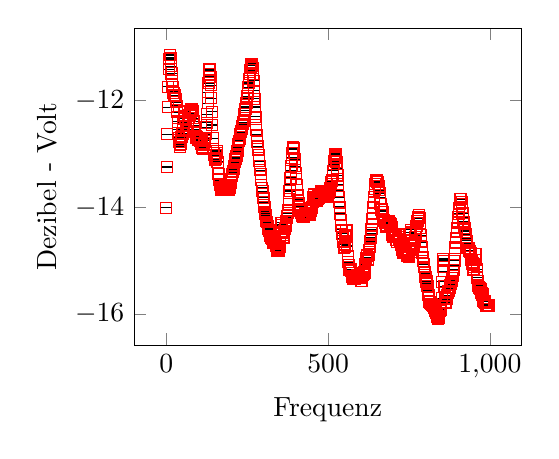
\begin{tikzpicture}
		\pgfplotsset{width=6.5cm,compat=1.3,legend style={font=\footnotesize}}
		\begin{axis}[xlabel={Frequenz},ylabel={Dezibel - Volt},legend cell align=left,legend pos=north west]
		\addplot+[only marks,color=red,mark=square,error bars/.cd,x dir=both,x explicit,y dir=both,y explicit,error bar style={color=black}] table[x=X,y=Y,x error=xerror,y error=yerror,row sep=\\]{
			X	Y	xerror	yerror	\\
			0.0	-14.004283	0	0	\\
			1.464844	-13.240946	0	0	\\
			2.929687	-12.627949	0	0	\\
			4.394531	-12.118516	0	0	\\
			5.859375	-11.735213	0	0	\\
			7.324219	-11.407348	0	0	\\
			8.789062	-11.224438	0	0	\\
			10.253906	-11.135541	0	0	\\
			11.71875	-11.146817	0	0	\\
			13.183594	-11.198439	0	0	\\
			14.648437	-11.353932	0	0	\\
			16.113281	-11.488094	0	0	\\
			17.578125	-11.63313	0	0	\\
			19.042969	-11.738722	0	0	\\
			20.507812	-11.816397	0	0	\\
			21.972656	-11.862113	0	0	\\
			23.4375	-11.89931	0	0	\\
			24.902344	-11.903909	0	0	\\
			26.367187	-11.896958	0	0	\\
			27.832031	-11.91789	0	0	\\
			29.296875	-11.964273	0	0	\\
			30.761719	-12.022869	0	0	\\
			32.226562	-12.095429	0	0	\\
			33.691406	-12.217092	0	0	\\
			35.15625	-12.389971	0	0	\\
			36.621094	-12.532281	0	0	\\
			38.085937	-12.695453	0	0	\\
			39.550781	-12.779384	0	0	\\
			41.015625	-12.864153	0	0	\\
			42.480469	-12.828726	0	0	\\
			43.945312	-12.812604	0	0	\\
			45.410156	-12.733512	0	0	\\
			46.875	-12.68038	0	0	\\
			48.339844	-12.664405	0	0	\\
			49.804687	-12.614113	0	0	\\
			51.269531	-12.542222	0	0	\\
			52.734375	-12.403173	0	0	\\
			54.199219	-12.287052	0	0	\\
			55.664062	-12.19136	0	0	\\
			57.128906	-12.215081	0	0	\\
			58.59375	-12.33298	0	0	\\
			60.058594	-12.475625	0	0	\\
			61.523437	-12.536543	0	0	\\
			62.988281	-12.560239	0	0	\\
			64.453125	-12.567647	0	0	\\
			65.917969	-12.475746	0	0	\\
			67.382812	-12.395083	0	0	\\
			68.847656	-12.328325	0	0	\\
			70.3125	-12.320772	0	0	\\
			71.777344	-12.276618	0	0	\\
			73.242187	-12.235891	0	0	\\
			74.707031	-12.21537	0	0	\\
			76.171875	-12.179939	0	0	\\
			77.636719	-12.163468	0	0	\\
			79.101562	-12.149996	0	0	\\
			80.566406	-12.18967	0	0	\\
			82.03125	-12.249993	0	0	\\
			83.496094	-12.326542	0	0	\\
			84.960937	-12.387578	0	0	\\
			86.425781	-12.456427	0	0	\\
			87.890625	-12.531565	0	0	\\
			89.355469	-12.589339	0	0	\\
			90.820312	-12.661935	0	0	\\
			92.285156	-12.704042	0	0	\\
			93.75	-12.67951	0	0	\\
			95.214844	-12.678006	0	0	\\
			96.679687	-12.709014	0	0	\\
			98.144531	-12.718855	0	0	\\
			99.609375	-12.738225	0	0	\\
			101.074219	-12.742752	0	0	\\
			102.539062	-12.742539	0	0	\\
			104.003906	-12.7485	0	0	\\
			105.46875	-12.72228	0	0	\\
			106.933594	-12.758915	0	0	\\
			108.398437	-12.814613	0	0	\\
			109.863281	-12.859919	0	0	\\
			111.328125	-12.874634	0	0	\\
			112.792969	-12.899707	0	0	\\
			114.257812	-12.89079	0	0	\\
			115.722656	-12.834525	0	0	\\
			117.1875	-12.787122	0	0	\\
			118.652344	-12.752169	0	0	\\
			120.117187	-12.693726	0	0	\\
			121.582031	-12.622843	0	0	\\
			123.046875	-12.49967	0	0	\\
			124.511719	-12.415074	0	0	\\
			125.976562	-12.253814	0	0	\\
			127.441406	-12.045887	0	0	\\
			128.90625	-11.83912	0	0	\\
			130.371094	-11.671799	0	0	\\
			131.835937	-11.50738	0	0	\\
			133.300781	-11.413431	0	0	\\
			134.765625	-11.423544	0	0	\\
			136.230469	-11.547593	0	0	\\
			137.695312	-11.711	0	0	\\
			139.160156	-11.950611	0	0	\\
			140.625	-12.20902	0	0	\\
			142.089844	-12.455142	0	0	\\
			143.554687	-12.699724	0	0	\\
			145.019531	-12.906923	0	0	\\
			146.484375	-12.973859	0	0	\\
			147.949219	-13.020177	0	0	\\
			149.414062	-13.078056	0	0	\\
			150.878906	-13.108562	0	0	\\
			152.34375	-13.097488	0	0	\\
			153.808594	-13.020356	0	0	\\
			155.273437	-12.940779	0	0	\\
			156.738281	-12.985352	0	0	\\
			158.203125	-13.144777	0	0	\\
			159.667969	-13.265233	0	0	\\
			161.132812	-13.369746	0	0	\\
			162.597656	-13.468094	0	0	\\
			164.0625	-13.490966	0	0	\\
			165.527344	-13.554856	0	0	\\
			166.992187	-13.585877	0	0	\\
			168.457031	-13.62068	0	0	\\
			169.921875	-13.670082	0	0	\\
			171.386719	-13.66189	0	0	\\
			172.851562	-13.640684	0	0	\\
			174.316406	-13.636638	0	0	\\
			175.78125	-13.614648	0	0	\\
			177.246094	-13.631992	0	0	\\
			178.710937	-13.630799	0	0	\\
			180.175781	-13.591036	0	0	\\
			181.640625	-13.572009	0	0	\\
			183.105469	-13.580378	0	0	\\
			184.570312	-13.598056	0	0	\\
			186.035156	-13.628461	0	0	\\
			187.5	-13.617635	0	0	\\
			188.964844	-13.620496	0	0	\\
			190.429687	-13.638085	0	0	\\
			191.894531	-13.652287	0	0	\\
			193.359375	-13.675512	0	0	\\
			194.824219	-13.670358	0	0	\\
			196.289062	-13.634846	0	0	\\
			197.753906	-13.601082	0	0	\\
			199.21875	-13.534634	0	0	\\
			200.683594	-13.472996	0	0	\\
			202.148437	-13.415578	0	0	\\
			203.613281	-13.378835	0	0	\\
			205.078125	-13.336044	0	0	\\
			206.542969	-13.310791	0	0	\\
			208.007812	-13.286436	0	0	\\
			209.472656	-13.217339	0	0	\\
			210.9375	-13.154947	0	0	\\
			212.402344	-13.108036	0	0	\\
			213.867187	-13.090161	0	0	\\
			215.332031	-13.069731	0	0	\\
			216.796875	-13.036578	0	0	\\
			218.261719	-12.991705	0	0	\\
			219.726562	-12.948761	0	0	\\
			221.191406	-12.870959	0	0	\\
			222.65625	-12.817556	0	0	\\
			224.121094	-12.748852	0	0	\\
			225.585937	-12.749967	0	0	\\
			227.050781	-12.713765	0	0	\\
			228.515625	-12.629536	0	0	\\
			229.980469	-12.589558	0	0	\\
			231.445312	-12.567836	0	0	\\
			232.910156	-12.522124	0	0	\\
			234.375	-12.468915	0	0	\\
			235.839844	-12.440714	0	0	\\
			237.304687	-12.399598	0	0	\\
			238.769531	-12.369069	0	0	\\
			240.234375	-12.326463	0	0	\\
			241.699219	-12.255556	0	0	\\
			243.164062	-12.180174	0	0	\\
			244.628906	-12.147997	0	0	\\
			246.09375	-12.115927	0	0	\\
			247.558594	-12.048352	0	0	\\
			249.023437	-11.96226	0	0	\\
			250.488281	-11.919503	0	0	\\
			251.953125	-11.871791	0	0	\\
			253.417969	-11.74577	0	0	\\
			254.882812	-11.666995	0	0	\\
			256.347656	-11.593143	0	0	\\
			257.8125	-11.490407	0	0	\\
			259.277344	-11.429134	0	0	\\
			260.742187	-11.374569	0	0	\\
			262.207031	-11.307126	0	0	\\
			263.671875	-11.304146	0	0	\\
			265.136719	-11.339795	0	0	\\
			266.601562	-11.385031	0	0	\\
			268.066406	-11.496305	0	0	\\
			269.53125	-11.62679	0	0	\\
			270.996094	-11.813617	0	0	\\
			272.460937	-11.963399	0	0	\\
			273.925781	-12.117005	0	0	\\
			275.390625	-12.299575	0	0	\\
			276.855469	-12.447815	0	0	\\
			278.320312	-12.550401	0	0	\\
			279.785156	-12.642071	0	0	\\
			281.25	-12.764309	0	0	\\
			282.714844	-12.858569	0	0	\\
			284.179687	-12.912494	0	0	\\
			285.644531	-13.023919	0	0	\\
			287.109375	-13.128728	0	0	\\
			288.574219	-13.225467	0	0	\\
			290.039062	-13.302616	0	0	\\
			291.503906	-13.376831	0	0	\\
			292.96875	-13.481067	0	0	\\
			294.433594	-13.630606	0	0	\\
			295.898437	-13.632221	0	0	\\
			297.363281	-13.695556	0	0	\\
			298.828125	-13.740269	0	0	\\
			300.292969	-13.817906	0	0	\\
			301.757812	-13.897342	0	0	\\
			303.222656	-13.98693	0	0	\\
			304.6875	-14.081668	0	0	\\
			306.152344	-14.112739	0	0	\\
			307.617187	-14.150769	0	0	\\
			309.082031	-14.243032	0	0	\\
			310.546875	-14.270702	0	0	\\
			312.011719	-14.272582	0	0	\\
			313.476562	-14.35026	0	0	\\
			314.941406	-14.401123	0	0	\\
			316.40625	-14.416316	0	0	\\
			317.871094	-14.432993	0	0	\\
			319.335937	-14.487273	0	0	\\
			320.800781	-14.535043	0	0	\\
			322.265625	-14.574156	0	0	\\
			323.730469	-14.564248	0	0	\\
			325.195312	-14.566572	0	0	\\
			326.660156	-14.557262	0	0	\\
			328.125	-14.590691	0	0	\\
			329.589844	-14.640462	0	0	\\
			331.054687	-14.657814	0	0	\\
			332.519531	-14.646799	0	0	\\
			333.984375	-14.636826	0	0	\\
			335.449219	-14.637593	0	0	\\
			336.914062	-14.667259	0	0	\\
			338.378906	-14.690057	0	0	\\
			339.84375	-14.716961	0	0	\\
			341.308594	-14.756373	0	0	\\
			342.773437	-14.807015	0	0	\\
			344.238281	-14.802729	0	0	\\
			345.703125	-14.787704	0	0	\\
			347.167969	-14.816484	0	0	\\
			348.632812	-14.763282	0	0	\\
			350.097656	-14.733747	0	0	\\
			351.5625	-14.642405	0	0	\\
			353.027344	-14.477943	0	0	\\
			354.492187	-14.323398	0	0	\\
			355.957031	-14.285539	0	0	\\
			357.421875	-14.337197	0	0	\\
			358.886719	-14.467901	0	0	\\
			360.351562	-14.554515	0	0	\\
			361.816406	-14.565249	0	0	\\
			363.28125	-14.506936	0	0	\\
			364.746094	-14.44492	0	0	\\
			366.210937	-14.408967	0	0	\\
			367.675781	-14.38543	0	0	\\
			369.140625	-14.339002	0	0	\\
			370.605469	-14.254098	0	0	\\
			372.070312	-14.192066	0	0	\\
			373.535156	-14.152829	0	0	\\
			375.0	-14.109365	0	0	\\
			376.464844	-14.0582	0	0	\\
			377.929687	-13.940236	0	0	\\
			379.394531	-13.835206	0	0	\\
			380.859375	-13.690187	0	0	\\
			382.324219	-13.567352	0	0	\\
			383.789062	-13.443974	0	0	\\
			385.253906	-13.313948	0	0	\\
			386.71875	-13.217422	0	0	\\
			388.183594	-13.073684	0	0	\\
			389.648437	-12.974572	0	0	\\
			391.113281	-12.90862	0	0	\\
			392.578125	-12.870437	0	0	\\
			394.042969	-12.894283	0	0	\\
			395.507812	-12.978061	0	0	\\
			396.972656	-13.094741	0	0	\\
			398.4375	-13.228979	0	0	\\
			399.902344	-13.35653	0	0	\\
			401.367187	-13.459676	0	0	\\
			402.832031	-13.576808	0	0	\\
			404.296875	-13.67802	0	0	\\
			405.761719	-13.770209	0	0	\\
			407.226562	-13.856529	0	0	\\
			408.691406	-13.926117	0	0	\\
			410.15625	-13.990658	0	0	\\
			411.621094	-14.036768	0	0	\\
			413.085937	-14.047368	0	0	\\
			414.550781	-14.06283	0	0	\\
			416.015625	-14.067854	0	0	\\
			417.480469	-14.104552	0	0	\\
			418.945312	-14.150084	0	0	\\
			420.410156	-14.159233	0	0	\\
			421.875	-14.180849	0	0	\\
			423.339844	-14.15247	0	0	\\
			424.804687	-14.174224	0	0	\\
			426.269531	-14.169175	0	0	\\
			427.734375	-14.147402	0	0	\\
			429.199219	-14.099271	0	0	\\
			430.664062	-14.097514	0	0	\\
			432.128906	-14.11475	0	0	\\
			433.59375	-14.135243	0	0	\\
			435.058594	-14.129529	0	0	\\
			436.523437	-14.13417	0	0	\\
			437.988281	-14.12454	0	0	\\
			439.453125	-14.144884	0	0	\\
			440.917969	-14.131666	0	0	\\
			442.382812	-14.146725	0	0	\\
			443.847656	-14.096645	0	0	\\
			445.3125	-14.073207	0	0	\\
			446.777344	-14.053824	0	0	\\
			448.242187	-14.011975	0	0	\\
			449.707031	-14.003206	0	0	\\
			451.171875	-13.994712	0	0	\\
			452.636719	-13.894277	0	0	\\
			454.101562	-13.814295	0	0	\\
			455.566406	-13.767425	0	0	\\
			457.03125	-13.741564	0	0	\\
			458.496094	-13.802678	0	0	\\
			459.960937	-13.860438	0	0	\\
			461.425781	-13.852045	0	0	\\
			462.890625	-13.851027	0	0	\\
			464.355469	-13.875035	0	0	\\
			465.820312	-13.83935	0	0	\\
			467.285156	-13.843899	0	0	\\
			468.75	-13.827202	0	0	\\
			470.214844	-13.785763	0	0	\\
			471.679687	-13.826627	0	0	\\
			473.144531	-13.789159	0	0	\\
			474.609375	-13.746697	0	0	\\
			476.074219	-13.740556	0	0	\\
			477.539062	-13.709714	0	0	\\
			479.003906	-13.701484	0	0	\\
			480.46875	-13.688481	0	0	\\
			481.933594	-13.685231	0	0	\\
			483.398437	-13.684994	0	0	\\
			484.863281	-13.68849	0	0	\\
			486.328125	-13.726487	0	0	\\
			487.792969	-13.758517	0	0	\\
			489.257812	-13.787527	0	0	\\
			490.722656	-13.774438	0	0	\\
			492.1875	-13.774698	0	0	\\
			493.652344	-13.794052	0	0	\\
			495.117187	-13.758289	0	0	\\
			496.582031	-13.782992	0	0	\\
			498.046875	-13.809293	0	0	\\
			499.511719	-13.746722	0	0	\\
			500.976562	-13.712915	0	0	\\
			502.441406	-13.704116	0	0	\\
			503.90625	-13.719003	0	0	\\
			505.371094	-13.663132	0	0	\\
			506.835937	-13.629186	0	0	\\
			508.300781	-13.566728	0	0	\\
			509.765625	-13.517934	0	0	\\
			511.230469	-13.508982	0	0	\\
			512.695312	-13.49075	0	0	\\
			514.160156	-13.392502	0	0	\\
			515.625	-13.31127	0	0	\\
			517.089844	-13.184895	0	0	\\
			518.554687	-13.126507	0	0	\\
			520.019531	-13.080378	0	0	\\
			521.484375	-13.019161	0	0	\\
			522.949219	-12.998055	0	0	\\
			524.414062	-13.045652	0	0	\\
			525.878906	-13.147205	0	0	\\
			527.34375	-13.267184	0	0	\\
			528.808594	-13.399378	0	0	\\
			530.273437	-13.563057	0	0	\\
			531.738281	-13.687705	0	0	\\
			533.203125	-13.807671	0	0	\\
			534.667969	-13.895032	0	0	\\
			536.132812	-13.988123	0	0	\\
			537.597656	-14.118769	0	0	\\
			539.0625	-14.240867	0	0	\\
			540.527344	-14.345597	0	0	\\
			541.992187	-14.420528	0	0	\\
			543.457031	-14.492039	0	0	\\
			544.921875	-14.573099	0	0	\\
			546.386719	-14.637138	0	0	\\
			547.851562	-14.733352	0	0	\\
			549.316406	-14.75538	0	0	\\
			550.78125	-14.745745	0	0	\\
			552.246094	-14.693775	0	0	\\
			553.710937	-14.526412	0	0	\\
			555.175781	-14.448621	0	0	\\
			556.640625	-14.430102	0	0	\\
			558.105469	-14.546825	0	0	\\
			559.570312	-14.721421	0	0	\\
			561.035156	-14.915332	0	0	\\
			562.5	-15.028123	0	0	\\
			563.964844	-15.086769	0	0	\\
			565.429687	-15.164866	0	0	\\
			566.894531	-15.162608	0	0	\\
			568.359375	-15.157296	0	0	\\
			569.824219	-15.158564	0	0	\\
			571.289062	-15.184606	0	0	\\
			572.753906	-15.227204	0	0	\\
			574.21875	-15.30381	0	0	\\
			575.683594	-15.334106	0	0	\\
			577.148437	-15.337667	0	0	\\
			578.613281	-15.327	0	0	\\
			580.078125	-15.337331	0	0	\\
			581.542969	-15.342279	0	0	\\
			583.007812	-15.321606	0	0	\\
			584.472656	-15.321913	0	0	\\
			585.9375	-15.322947	0	0	\\
			587.402344	-15.307792	0	0	\\
			588.867187	-15.28635	0	0	\\
			590.332031	-15.275439	0	0	\\
			591.796875	-15.265609	0	0	\\
			593.261719	-15.292857	0	0	\\
			594.726562	-15.281776	0	0	\\
			596.191406	-15.305321	0	0	\\
			597.65625	-15.315447	0	0	\\
			599.121094	-15.328534	0	0	\\
			600.585937	-15.327209	0	0	\\
			602.050781	-15.37632	0	0	\\
			603.515625	-15.373119	0	0	\\
			604.980469	-15.312519	0	0	\\
			606.445312	-15.254641	0	0	\\
			607.910156	-15.271929	0	0	\\
			609.375	-15.237128	0	0	\\
			610.839844	-15.225204	0	0	\\
			612.304687	-15.219803	0	0	\\
			613.769531	-15.143885	0	0	\\
			615.234375	-15.059427	0	0	\\
			616.699219	-14.987514	0	0	\\
			618.164062	-14.939815	0	0	\\
			619.628906	-14.901828	0	0	\\
			621.09375	-14.900862	0	0	\\
			622.558594	-14.969786	0	0	\\
			624.023437	-14.977024	0	0	\\
			625.488281	-14.881377	0	0	\\
			626.953125	-14.79333	0	0	\\
			628.417969	-14.729989	0	0	\\
			629.882812	-14.62785	0	0	\\
			631.347656	-14.561667	0	0	\\
			632.8125	-14.486842	0	0	\\
			634.277344	-14.408578	0	0	\\
			635.742187	-14.326564	0	0	\\
			637.207031	-14.222596	0	0	\\
			638.671875	-14.110782	0	0	\\
			640.136719	-13.997792	0	0	\\
			641.601562	-13.907137	0	0	\\
			643.066406	-13.804422	0	0	\\
			644.53125	-13.658062	0	0	\\
			645.996094	-13.560715	0	0	\\
			647.460937	-13.5009	0	0	\\
			648.925781	-13.495064	0	0	\\
			650.390625	-13.514473	0	0	\\
			651.855469	-13.490421	0	0	\\
			653.320312	-13.527529	0	0	\\
			654.785156	-13.564345	0	0	\\
			656.25	-13.604566	0	0	\\
			657.714844	-13.677679	0	0	\\
			659.179687	-13.735968	0	0	\\
			660.644531	-13.820734	0	0	\\
			662.109375	-13.929063	0	0	\\
			663.574219	-14.050467	0	0	\\
			665.039062	-14.033894	0	0	\\
			666.503906	-14.051598	0	0	\\
			667.96875	-14.08037	0	0	\\
			669.433594	-14.133394	0	0	\\
			670.898437	-14.220636	0	0	\\
			672.363281	-14.23358	0	0	\\
			673.828125	-14.259767	0	0	\\
			675.292969	-14.285292	0	0	\\
			676.757812	-14.282202	0	0	\\
			678.222656	-14.321799	0	0	\\
			679.6875	-14.356291	0	0	\\
			681.152344	-14.350688	0	0	\\
			682.617187	-14.327687	0	0	\\
			684.082031	-14.287823	0	0	\\
			685.546875	-14.298334	0	0	\\
			687.011719	-14.281334	0	0	\\
			688.476562	-14.250317	0	0	\\
			689.941406	-14.287738	0	0	\\
			691.40625	-14.303469	0	0	\\
			692.871094	-14.323131	0	0	\\
			694.335937	-14.319679	0	0	\\
			695.800781	-14.359524	0	0	\\
			697.265625	-14.428386	0	0	\\
			698.730469	-14.512695	0	0	\\
			700.195312	-14.535693	0	0	\\
			701.660156	-14.544378	0	0	\\
			703.125	-14.546101	0	0	\\
			704.589844	-14.502697	0	0	\\
			706.054687	-14.502353	0	0	\\
			707.519531	-14.512217	0	0	\\
			708.984375	-14.532339	0	0	\\
			710.449219	-14.606031	0	0	\\
			711.914062	-14.648579	0	0	\\
			713.378906	-14.608194	0	0	\\
			714.84375	-14.549568	0	0	\\
			716.308594	-14.494463	0	0	\\
			717.773437	-14.521065	0	0	\\
			719.238281	-14.521839	0	0	\\
			720.703125	-14.584913	0	0	\\
			722.167969	-14.634155	0	0	\\
			723.632812	-14.645411	0	0	\\
			725.097656	-14.683364	0	0	\\
			726.5625	-14.701651	0	0	\\
			728.027344	-14.745538	0	0	\\
			729.492187	-14.787056	0	0	\\
			730.957031	-14.847834	0	0	\\
			732.421875	-14.839916	0	0	\\
			733.886719	-14.834844	0	0	\\
			735.351562	-14.834649	0	0	\\
			736.816406	-14.838762	0	0	\\
			738.28125	-14.832234	0	0	\\
			739.746094	-14.817942	0	0	\\
			741.210937	-14.848742	0	0	\\
			742.675781	-14.879172	0	0	\\
			744.140625	-14.9148	0	0	\\
			745.605469	-14.880893	0	0	\\
			747.070312	-14.907684	0	0	\\
			748.535156	-14.909078	0	0	\\
			750.0	-14.924667	0	0	\\
			751.464844	-14.791975	0	0	\\
			752.929687	-14.665897	0	0	\\
			754.394531	-14.504931	0	0	\\
			755.859375	-14.414902	0	0	\\
			757.324219	-14.469764	0	0	\\
			758.789062	-14.616367	0	0	\\
			760.253906	-14.771271	0	0	\\
			761.71875	-14.825436	0	0	\\
			763.183594	-14.781694	0	0	\\
			764.648437	-14.729776	0	0	\\
			766.113281	-14.673937	0	0	\\
			767.578125	-14.608036	0	0	\\
			769.042969	-14.553159	0	0	\\
			770.507812	-14.487487	0	0	\\
			771.972656	-14.442209	0	0	\\
			773.4375	-14.353952	0	0	\\
			774.902344	-14.286075	0	0	\\
			776.367187	-14.256886	0	0	\\
			777.832031	-14.208799	0	0	\\
			779.296875	-14.187906	0	0	\\
			780.761719	-14.148963	0	0	\\
			782.226562	-14.194851	0	0	\\
			783.691406	-14.28554	0	0	\\
			785.15625	-14.389358	0	0	\\
			786.621094	-14.524423	0	0	\\
			788.085937	-14.648572	0	0	\\
			789.550781	-14.737702	0	0	\\
			791.015625	-14.842474	0	0	\\
			792.480469	-14.936387	0	0	\\
			793.945312	-15.005563	0	0	\\
			795.410156	-15.0598	0	0	\\
			796.875	-15.118703	0	0	\\
			798.339844	-15.208051	0	0	\\
			799.804687	-15.234525	0	0	\\
			801.269531	-15.299216	0	0	\\
			802.734375	-15.364965	0	0	\\
			804.199219	-15.387265	0	0	\\
			805.664062	-15.414881	0	0	\\
			807.128906	-15.475559	0	0	\\
			808.59375	-15.55237	0	0	\\
			810.058594	-15.643153	0	0	\\
			811.523437	-15.701274	0	0	\\
			812.988281	-15.761165	0	0	\\
			814.453125	-15.766149	0	0	\\
			815.917969	-15.780131	0	0	\\
			817.382812	-15.803351	0	0	\\
			818.847656	-15.814104	0	0	\\
			820.3125	-15.8027	0	0	\\
			821.777344	-15.819212	0	0	\\
			823.242187	-15.836081	0	0	\\
			824.707031	-15.836153	0	0	\\
			826.171875	-15.856551	0	0	\\
			827.636719	-15.883613	0	0	\\
			829.101562	-15.869967	0	0	\\
			830.566406	-15.923962	0	0	\\
			832.03125	-15.940643	0	0	\\
			833.496094	-15.961584	0	0	\\
			834.960937	-15.971349	0	0	\\
			836.425781	-16.001772	0	0	\\
			837.890625	-16.04227	0	0	\\
			839.355469	-16.078202	0	0	\\
			840.820312	-16.084716	0	0	\\
			842.285156	-16.075089	0	0	\\
			843.75	-16.004776	0	0	\\
			845.214844	-15.942141	0	0	\\
			846.679687	-15.904643	0	0	\\
			848.144531	-15.917102	0	0	\\
			849.609375	-15.872845	0	0	\\
			851.074219	-15.703421	0	0	\\
			852.539062	-15.392884	0	0	\\
			854.003906	-15.109339	0	0	\\
			855.46875	-14.965858	0	0	\\
			856.933594	-14.998689	0	0	\\
			858.398437	-15.197996	0	0	\\
			859.863281	-15.478261	0	0	\\
			861.328125	-15.720332	0	0	\\
			862.792969	-15.795883	0	0	\\
			864.257812	-15.77294	0	0	\\
			865.722656	-15.704719	0	0	\\
			867.1875	-15.657263	0	0	\\
			868.652344	-15.646527	0	0	\\
			870.117187	-15.59701	0	0	\\
			871.582031	-15.562216	0	0	\\
			873.046875	-15.557948	0	0	\\
			874.511719	-15.559016	0	0	\\
			875.976562	-15.515398	0	0	\\
			877.441406	-15.447929	0	0	\\
			878.90625	-15.441718	0	0	\\
			880.371094	-15.400484	0	0	\\
			881.835937	-15.376469	0	0	\\
			883.300781	-15.31872	0	0	\\
			884.765625	-15.291627	0	0	\\
			886.230469	-15.213386	0	0	\\
			887.695312	-15.168859	0	0	\\
			889.160156	-15.081033	0	0	\\
			890.625	-15.000439	0	0	\\
			892.089844	-14.867262	0	0	\\
			893.554687	-14.750787	0	0	\\
			895.019531	-14.646878	0	0	\\
			896.484375	-14.57057	0	0	\\
			897.949219	-14.465515	0	0	\\
			899.414062	-14.383338	0	0	\\
			900.878906	-14.281526	0	0	\\
			902.34375	-14.187008	0	0	\\
			903.808594	-14.11856	0	0	\\
			905.273437	-14.020703	0	0	\\
			906.738281	-13.931706	0	0	\\
			908.203125	-13.850057	0	0	\\
			909.667969	-13.842437	0	0	\\
			911.132812	-13.843392	0	0	\\
			912.597656	-13.905562	0	0	\\
			914.0625	-13.998379	0	0	\\
			915.527344	-14.108174	0	0	\\
			916.992187	-14.194473	0	0	\\
			918.457031	-14.271071	0	0	\\
			919.921875	-14.306465	0	0	\\
			921.386719	-14.386424	0	0	\\
			922.851562	-14.425389	0	0	\\
			924.316406	-14.456845	0	0	\\
			925.78125	-14.498443	0	0	\\
			927.246094	-14.583064	0	0	\\
			928.710937	-14.624491	0	0	\\
			930.175781	-14.669604	0	0	\\
			931.640625	-14.753962	0	0	\\
			933.105469	-14.7567	0	0	\\
			934.570312	-14.762024	0	0	\\
			936.035156	-14.811727	0	0	\\
			937.5	-14.813593	0	0	\\
			938.964844	-14.82591	0	0	\\
			940.429687	-14.86176	0	0	\\
			941.894531	-14.920625	0	0	\\
			943.359375	-14.979934	0	0	\\
			944.824219	-15.013484	0	0	\\
			946.289062	-15.048883	0	0	\\
			947.753906	-15.117895	0	0	\\
			949.21875	-15.172387	0	0	\\
			950.683594	-15.147505	0	0	\\
			952.148437	-15.07019	0	0	\\
			953.613281	-14.978779	0	0	\\
			955.078125	-14.879593	0	0	\\
			956.542969	-14.879584	0	0	\\
			958.007812	-14.982322	0	0	\\
			959.472656	-15.16314	0	0	\\
			960.9375	-15.313421	0	0	\\
			962.402344	-15.382834	0	0	\\
			963.867187	-15.462441	0	0	\\
			965.332031	-15.488177	0	0	\\
			966.796875	-15.511868	0	0	\\
			968.261719	-15.521721	0	0	\\
			969.726562	-15.509936	0	0	\\
			971.191406	-15.530067	0	0	\\
			972.65625	-15.552961	0	0	\\
			974.121094	-15.601632	0	0	\\
			975.585937	-15.62226	0	0	\\
			977.050781	-15.631798	0	0	\\
			978.515625	-15.697486	0	0	\\
			979.980469	-15.753755	0	0	\\
			981.445312	-15.765028	0	0	\\
			982.910156	-15.746485	0	0	\\
			984.375	-15.757503	0	0	\\
			985.839844	-15.793394	0	0	\\
			987.304687	-15.820141	0	0	\\
			988.769531	-15.836665	0	0	\\
			990.234375	-15.838643	0	0	\\
			991.699219	-15.845026	0	0	\\
			993.164062	-15.835679	0	0	\\
			994.628906	-15.835999	0	0	\\
			996.09375	-15.842127	0	0	\\
			997.558594	-15.831357	0	0	\\
		};		% \addlegendentry{Messpunkte Datensatz 0}
		\end{axis}
		\end{tikzpicture}
	\caption{Umgebung}
	\label{fig:Umgebungsmessung}
\end{figure}
            \begin{figure}[H]
	\centering
	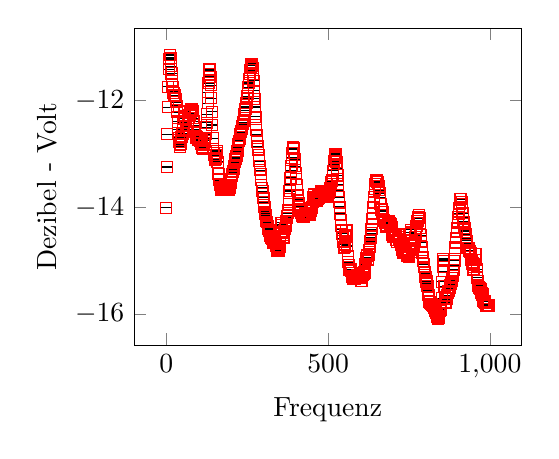
\begin{tikzpicture}
		\pgfplotsset{width=6.5cm,compat=1.3,legend style={font=\footnotesize}}
		\begin{axis}[xlabel={Frequenz},ylabel={Dezibel - Volt},legend cell align=left,legend pos=north west]
		\addplot+[only marks,color=red,mark=square,error bars/.cd,x dir=both,x explicit,y dir=both,y explicit,error bar style={color=black}] table[x=X,y=Y,x error=xerror,y error=yerror,row sep=\\]{
			X	Y	xerror	yerror	\\
			0.0	-14.004283	0	0	\\
			1.464844	-13.240946	0	0	\\
			2.929687	-12.627949	0	0	\\
			4.394531	-12.118516	0	0	\\
			5.859375	-11.735213	0	0	\\
			7.324219	-11.407348	0	0	\\
			8.789062	-11.224438	0	0	\\
			10.253906	-11.135541	0	0	\\
			11.71875	-11.146817	0	0	\\
			13.183594	-11.198439	0	0	\\
			14.648437	-11.353932	0	0	\\
			16.113281	-11.488094	0	0	\\
			17.578125	-11.63313	0	0	\\
			19.042969	-11.738722	0	0	\\
			20.507812	-11.816397	0	0	\\
			21.972656	-11.862113	0	0	\\
			23.4375	-11.89931	0	0	\\
			24.902344	-11.903909	0	0	\\
			26.367187	-11.896958	0	0	\\
			27.832031	-11.91789	0	0	\\
			29.296875	-11.964273	0	0	\\
			30.761719	-12.022869	0	0	\\
			32.226562	-12.095429	0	0	\\
			33.691406	-12.217092	0	0	\\
			35.15625	-12.389971	0	0	\\
			36.621094	-12.532281	0	0	\\
			38.085937	-12.695453	0	0	\\
			39.550781	-12.779384	0	0	\\
			41.015625	-12.864153	0	0	\\
			42.480469	-12.828726	0	0	\\
			43.945312	-12.812604	0	0	\\
			45.410156	-12.733512	0	0	\\
			46.875	-12.68038	0	0	\\
			48.339844	-12.664405	0	0	\\
			49.804687	-12.614113	0	0	\\
			51.269531	-12.542222	0	0	\\
			52.734375	-12.403173	0	0	\\
			54.199219	-12.287052	0	0	\\
			55.664062	-12.19136	0	0	\\
			57.128906	-12.215081	0	0	\\
			58.59375	-12.33298	0	0	\\
			60.058594	-12.475625	0	0	\\
			61.523437	-12.536543	0	0	\\
			62.988281	-12.560239	0	0	\\
			64.453125	-12.567647	0	0	\\
			65.917969	-12.475746	0	0	\\
			67.382812	-12.395083	0	0	\\
			68.847656	-12.328325	0	0	\\
			70.3125	-12.320772	0	0	\\
			71.777344	-12.276618	0	0	\\
			73.242187	-12.235891	0	0	\\
			74.707031	-12.21537	0	0	\\
			76.171875	-12.179939	0	0	\\
			77.636719	-12.163468	0	0	\\
			79.101562	-12.149996	0	0	\\
			80.566406	-12.18967	0	0	\\
			82.03125	-12.249993	0	0	\\
			83.496094	-12.326542	0	0	\\
			84.960937	-12.387578	0	0	\\
			86.425781	-12.456427	0	0	\\
			87.890625	-12.531565	0	0	\\
			89.355469	-12.589339	0	0	\\
			90.820312	-12.661935	0	0	\\
			92.285156	-12.704042	0	0	\\
			93.75	-12.67951	0	0	\\
			95.214844	-12.678006	0	0	\\
			96.679687	-12.709014	0	0	\\
			98.144531	-12.718855	0	0	\\
			99.609375	-12.738225	0	0	\\
			101.074219	-12.742752	0	0	\\
			102.539062	-12.742539	0	0	\\
			104.003906	-12.7485	0	0	\\
			105.46875	-12.72228	0	0	\\
			106.933594	-12.758915	0	0	\\
			108.398437	-12.814613	0	0	\\
			109.863281	-12.859919	0	0	\\
			111.328125	-12.874634	0	0	\\
			112.792969	-12.899707	0	0	\\
			114.257812	-12.89079	0	0	\\
			115.722656	-12.834525	0	0	\\
			117.1875	-12.787122	0	0	\\
			118.652344	-12.752169	0	0	\\
			120.117187	-12.693726	0	0	\\
			121.582031	-12.622843	0	0	\\
			123.046875	-12.49967	0	0	\\
			124.511719	-12.415074	0	0	\\
			125.976562	-12.253814	0	0	\\
			127.441406	-12.045887	0	0	\\
			128.90625	-11.83912	0	0	\\
			130.371094	-11.671799	0	0	\\
			131.835937	-11.50738	0	0	\\
			133.300781	-11.413431	0	0	\\
			134.765625	-11.423544	0	0	\\
			136.230469	-11.547593	0	0	\\
			137.695312	-11.711	0	0	\\
			139.160156	-11.950611	0	0	\\
			140.625	-12.20902	0	0	\\
			142.089844	-12.455142	0	0	\\
			143.554687	-12.699724	0	0	\\
			145.019531	-12.906923	0	0	\\
			146.484375	-12.973859	0	0	\\
			147.949219	-13.020177	0	0	\\
			149.414062	-13.078056	0	0	\\
			150.878906	-13.108562	0	0	\\
			152.34375	-13.097488	0	0	\\
			153.808594	-13.020356	0	0	\\
			155.273437	-12.940779	0	0	\\
			156.738281	-12.985352	0	0	\\
			158.203125	-13.144777	0	0	\\
			159.667969	-13.265233	0	0	\\
			161.132812	-13.369746	0	0	\\
			162.597656	-13.468094	0	0	\\
			164.0625	-13.490966	0	0	\\
			165.527344	-13.554856	0	0	\\
			166.992187	-13.585877	0	0	\\
			168.457031	-13.62068	0	0	\\
			169.921875	-13.670082	0	0	\\
			171.386719	-13.66189	0	0	\\
			172.851562	-13.640684	0	0	\\
			174.316406	-13.636638	0	0	\\
			175.78125	-13.614648	0	0	\\
			177.246094	-13.631992	0	0	\\
			178.710937	-13.630799	0	0	\\
			180.175781	-13.591036	0	0	\\
			181.640625	-13.572009	0	0	\\
			183.105469	-13.580378	0	0	\\
			184.570312	-13.598056	0	0	\\
			186.035156	-13.628461	0	0	\\
			187.5	-13.617635	0	0	\\
			188.964844	-13.620496	0	0	\\
			190.429687	-13.638085	0	0	\\
			191.894531	-13.652287	0	0	\\
			193.359375	-13.675512	0	0	\\
			194.824219	-13.670358	0	0	\\
			196.289062	-13.634846	0	0	\\
			197.753906	-13.601082	0	0	\\
			199.21875	-13.534634	0	0	\\
			200.683594	-13.472996	0	0	\\
			202.148437	-13.415578	0	0	\\
			203.613281	-13.378835	0	0	\\
			205.078125	-13.336044	0	0	\\
			206.542969	-13.310791	0	0	\\
			208.007812	-13.286436	0	0	\\
			209.472656	-13.217339	0	0	\\
			210.9375	-13.154947	0	0	\\
			212.402344	-13.108036	0	0	\\
			213.867187	-13.090161	0	0	\\
			215.332031	-13.069731	0	0	\\
			216.796875	-13.036578	0	0	\\
			218.261719	-12.991705	0	0	\\
			219.726562	-12.948761	0	0	\\
			221.191406	-12.870959	0	0	\\
			222.65625	-12.817556	0	0	\\
			224.121094	-12.748852	0	0	\\
			225.585937	-12.749967	0	0	\\
			227.050781	-12.713765	0	0	\\
			228.515625	-12.629536	0	0	\\
			229.980469	-12.589558	0	0	\\
			231.445312	-12.567836	0	0	\\
			232.910156	-12.522124	0	0	\\
			234.375	-12.468915	0	0	\\
			235.839844	-12.440714	0	0	\\
			237.304687	-12.399598	0	0	\\
			238.769531	-12.369069	0	0	\\
			240.234375	-12.326463	0	0	\\
			241.699219	-12.255556	0	0	\\
			243.164062	-12.180174	0	0	\\
			244.628906	-12.147997	0	0	\\
			246.09375	-12.115927	0	0	\\
			247.558594	-12.048352	0	0	\\
			249.023437	-11.96226	0	0	\\
			250.488281	-11.919503	0	0	\\
			251.953125	-11.871791	0	0	\\
			253.417969	-11.74577	0	0	\\
			254.882812	-11.666995	0	0	\\
			256.347656	-11.593143	0	0	\\
			257.8125	-11.490407	0	0	\\
			259.277344	-11.429134	0	0	\\
			260.742187	-11.374569	0	0	\\
			262.207031	-11.307126	0	0	\\
			263.671875	-11.304146	0	0	\\
			265.136719	-11.339795	0	0	\\
			266.601562	-11.385031	0	0	\\
			268.066406	-11.496305	0	0	\\
			269.53125	-11.62679	0	0	\\
			270.996094	-11.813617	0	0	\\
			272.460937	-11.963399	0	0	\\
			273.925781	-12.117005	0	0	\\
			275.390625	-12.299575	0	0	\\
			276.855469	-12.447815	0	0	\\
			278.320312	-12.550401	0	0	\\
			279.785156	-12.642071	0	0	\\
			281.25	-12.764309	0	0	\\
			282.714844	-12.858569	0	0	\\
			284.179687	-12.912494	0	0	\\
			285.644531	-13.023919	0	0	\\
			287.109375	-13.128728	0	0	\\
			288.574219	-13.225467	0	0	\\
			290.039062	-13.302616	0	0	\\
			291.503906	-13.376831	0	0	\\
			292.96875	-13.481067	0	0	\\
			294.433594	-13.630606	0	0	\\
			295.898437	-13.632221	0	0	\\
			297.363281	-13.695556	0	0	\\
			298.828125	-13.740269	0	0	\\
			300.292969	-13.817906	0	0	\\
			301.757812	-13.897342	0	0	\\
			303.222656	-13.98693	0	0	\\
			304.6875	-14.081668	0	0	\\
			306.152344	-14.112739	0	0	\\
			307.617187	-14.150769	0	0	\\
			309.082031	-14.243032	0	0	\\
			310.546875	-14.270702	0	0	\\
			312.011719	-14.272582	0	0	\\
			313.476562	-14.35026	0	0	\\
			314.941406	-14.401123	0	0	\\
			316.40625	-14.416316	0	0	\\
			317.871094	-14.432993	0	0	\\
			319.335937	-14.487273	0	0	\\
			320.800781	-14.535043	0	0	\\
			322.265625	-14.574156	0	0	\\
			323.730469	-14.564248	0	0	\\
			325.195312	-14.566572	0	0	\\
			326.660156	-14.557262	0	0	\\
			328.125	-14.590691	0	0	\\
			329.589844	-14.640462	0	0	\\
			331.054687	-14.657814	0	0	\\
			332.519531	-14.646799	0	0	\\
			333.984375	-14.636826	0	0	\\
			335.449219	-14.637593	0	0	\\
			336.914062	-14.667259	0	0	\\
			338.378906	-14.690057	0	0	\\
			339.84375	-14.716961	0	0	\\
			341.308594	-14.756373	0	0	\\
			342.773437	-14.807015	0	0	\\
			344.238281	-14.802729	0	0	\\
			345.703125	-14.787704	0	0	\\
			347.167969	-14.816484	0	0	\\
			348.632812	-14.763282	0	0	\\
			350.097656	-14.733747	0	0	\\
			351.5625	-14.642405	0	0	\\
			353.027344	-14.477943	0	0	\\
			354.492187	-14.323398	0	0	\\
			355.957031	-14.285539	0	0	\\
			357.421875	-14.337197	0	0	\\
			358.886719	-14.467901	0	0	\\
			360.351562	-14.554515	0	0	\\
			361.816406	-14.565249	0	0	\\
			363.28125	-14.506936	0	0	\\
			364.746094	-14.44492	0	0	\\
			366.210937	-14.408967	0	0	\\
			367.675781	-14.38543	0	0	\\
			369.140625	-14.339002	0	0	\\
			370.605469	-14.254098	0	0	\\
			372.070312	-14.192066	0	0	\\
			373.535156	-14.152829	0	0	\\
			375.0	-14.109365	0	0	\\
			376.464844	-14.0582	0	0	\\
			377.929687	-13.940236	0	0	\\
			379.394531	-13.835206	0	0	\\
			380.859375	-13.690187	0	0	\\
			382.324219	-13.567352	0	0	\\
			383.789062	-13.443974	0	0	\\
			385.253906	-13.313948	0	0	\\
			386.71875	-13.217422	0	0	\\
			388.183594	-13.073684	0	0	\\
			389.648437	-12.974572	0	0	\\
			391.113281	-12.90862	0	0	\\
			392.578125	-12.870437	0	0	\\
			394.042969	-12.894283	0	0	\\
			395.507812	-12.978061	0	0	\\
			396.972656	-13.094741	0	0	\\
			398.4375	-13.228979	0	0	\\
			399.902344	-13.35653	0	0	\\
			401.367187	-13.459676	0	0	\\
			402.832031	-13.576808	0	0	\\
			404.296875	-13.67802	0	0	\\
			405.761719	-13.770209	0	0	\\
			407.226562	-13.856529	0	0	\\
			408.691406	-13.926117	0	0	\\
			410.15625	-13.990658	0	0	\\
			411.621094	-14.036768	0	0	\\
			413.085937	-14.047368	0	0	\\
			414.550781	-14.06283	0	0	\\
			416.015625	-14.067854	0	0	\\
			417.480469	-14.104552	0	0	\\
			418.945312	-14.150084	0	0	\\
			420.410156	-14.159233	0	0	\\
			421.875	-14.180849	0	0	\\
			423.339844	-14.15247	0	0	\\
			424.804687	-14.174224	0	0	\\
			426.269531	-14.169175	0	0	\\
			427.734375	-14.147402	0	0	\\
			429.199219	-14.099271	0	0	\\
			430.664062	-14.097514	0	0	\\
			432.128906	-14.11475	0	0	\\
			433.59375	-14.135243	0	0	\\
			435.058594	-14.129529	0	0	\\
			436.523437	-14.13417	0	0	\\
			437.988281	-14.12454	0	0	\\
			439.453125	-14.144884	0	0	\\
			440.917969	-14.131666	0	0	\\
			442.382812	-14.146725	0	0	\\
			443.847656	-14.096645	0	0	\\
			445.3125	-14.073207	0	0	\\
			446.777344	-14.053824	0	0	\\
			448.242187	-14.011975	0	0	\\
			449.707031	-14.003206	0	0	\\
			451.171875	-13.994712	0	0	\\
			452.636719	-13.894277	0	0	\\
			454.101562	-13.814295	0	0	\\
			455.566406	-13.767425	0	0	\\
			457.03125	-13.741564	0	0	\\
			458.496094	-13.802678	0	0	\\
			459.960937	-13.860438	0	0	\\
			461.425781	-13.852045	0	0	\\
			462.890625	-13.851027	0	0	\\
			464.355469	-13.875035	0	0	\\
			465.820312	-13.83935	0	0	\\
			467.285156	-13.843899	0	0	\\
			468.75	-13.827202	0	0	\\
			470.214844	-13.785763	0	0	\\
			471.679687	-13.826627	0	0	\\
			473.144531	-13.789159	0	0	\\
			474.609375	-13.746697	0	0	\\
			476.074219	-13.740556	0	0	\\
			477.539062	-13.709714	0	0	\\
			479.003906	-13.701484	0	0	\\
			480.46875	-13.688481	0	0	\\
			481.933594	-13.685231	0	0	\\
			483.398437	-13.684994	0	0	\\
			484.863281	-13.68849	0	0	\\
			486.328125	-13.726487	0	0	\\
			487.792969	-13.758517	0	0	\\
			489.257812	-13.787527	0	0	\\
			490.722656	-13.774438	0	0	\\
			492.1875	-13.774698	0	0	\\
			493.652344	-13.794052	0	0	\\
			495.117187	-13.758289	0	0	\\
			496.582031	-13.782992	0	0	\\
			498.046875	-13.809293	0	0	\\
			499.511719	-13.746722	0	0	\\
			500.976562	-13.712915	0	0	\\
			502.441406	-13.704116	0	0	\\
			503.90625	-13.719003	0	0	\\
			505.371094	-13.663132	0	0	\\
			506.835937	-13.629186	0	0	\\
			508.300781	-13.566728	0	0	\\
			509.765625	-13.517934	0	0	\\
			511.230469	-13.508982	0	0	\\
			512.695312	-13.49075	0	0	\\
			514.160156	-13.392502	0	0	\\
			515.625	-13.31127	0	0	\\
			517.089844	-13.184895	0	0	\\
			518.554687	-13.126507	0	0	\\
			520.019531	-13.080378	0	0	\\
			521.484375	-13.019161	0	0	\\
			522.949219	-12.998055	0	0	\\
			524.414062	-13.045652	0	0	\\
			525.878906	-13.147205	0	0	\\
			527.34375	-13.267184	0	0	\\
			528.808594	-13.399378	0	0	\\
			530.273437	-13.563057	0	0	\\
			531.738281	-13.687705	0	0	\\
			533.203125	-13.807671	0	0	\\
			534.667969	-13.895032	0	0	\\
			536.132812	-13.988123	0	0	\\
			537.597656	-14.118769	0	0	\\
			539.0625	-14.240867	0	0	\\
			540.527344	-14.345597	0	0	\\
			541.992187	-14.420528	0	0	\\
			543.457031	-14.492039	0	0	\\
			544.921875	-14.573099	0	0	\\
			546.386719	-14.637138	0	0	\\
			547.851562	-14.733352	0	0	\\
			549.316406	-14.75538	0	0	\\
			550.78125	-14.745745	0	0	\\
			552.246094	-14.693775	0	0	\\
			553.710937	-14.526412	0	0	\\
			555.175781	-14.448621	0	0	\\
			556.640625	-14.430102	0	0	\\
			558.105469	-14.546825	0	0	\\
			559.570312	-14.721421	0	0	\\
			561.035156	-14.915332	0	0	\\
			562.5	-15.028123	0	0	\\
			563.964844	-15.086769	0	0	\\
			565.429687	-15.164866	0	0	\\
			566.894531	-15.162608	0	0	\\
			568.359375	-15.157296	0	0	\\
			569.824219	-15.158564	0	0	\\
			571.289062	-15.184606	0	0	\\
			572.753906	-15.227204	0	0	\\
			574.21875	-15.30381	0	0	\\
			575.683594	-15.334106	0	0	\\
			577.148437	-15.337667	0	0	\\
			578.613281	-15.327	0	0	\\
			580.078125	-15.337331	0	0	\\
			581.542969	-15.342279	0	0	\\
			583.007812	-15.321606	0	0	\\
			584.472656	-15.321913	0	0	\\
			585.9375	-15.322947	0	0	\\
			587.402344	-15.307792	0	0	\\
			588.867187	-15.28635	0	0	\\
			590.332031	-15.275439	0	0	\\
			591.796875	-15.265609	0	0	\\
			593.261719	-15.292857	0	0	\\
			594.726562	-15.281776	0	0	\\
			596.191406	-15.305321	0	0	\\
			597.65625	-15.315447	0	0	\\
			599.121094	-15.328534	0	0	\\
			600.585937	-15.327209	0	0	\\
			602.050781	-15.37632	0	0	\\
			603.515625	-15.373119	0	0	\\
			604.980469	-15.312519	0	0	\\
			606.445312	-15.254641	0	0	\\
			607.910156	-15.271929	0	0	\\
			609.375	-15.237128	0	0	\\
			610.839844	-15.225204	0	0	\\
			612.304687	-15.219803	0	0	\\
			613.769531	-15.143885	0	0	\\
			615.234375	-15.059427	0	0	\\
			616.699219	-14.987514	0	0	\\
			618.164062	-14.939815	0	0	\\
			619.628906	-14.901828	0	0	\\
			621.09375	-14.900862	0	0	\\
			622.558594	-14.969786	0	0	\\
			624.023437	-14.977024	0	0	\\
			625.488281	-14.881377	0	0	\\
			626.953125	-14.79333	0	0	\\
			628.417969	-14.729989	0	0	\\
			629.882812	-14.62785	0	0	\\
			631.347656	-14.561667	0	0	\\
			632.8125	-14.486842	0	0	\\
			634.277344	-14.408578	0	0	\\
			635.742187	-14.326564	0	0	\\
			637.207031	-14.222596	0	0	\\
			638.671875	-14.110782	0	0	\\
			640.136719	-13.997792	0	0	\\
			641.601562	-13.907137	0	0	\\
			643.066406	-13.804422	0	0	\\
			644.53125	-13.658062	0	0	\\
			645.996094	-13.560715	0	0	\\
			647.460937	-13.5009	0	0	\\
			648.925781	-13.495064	0	0	\\
			650.390625	-13.514473	0	0	\\
			651.855469	-13.490421	0	0	\\
			653.320312	-13.527529	0	0	\\
			654.785156	-13.564345	0	0	\\
			656.25	-13.604566	0	0	\\
			657.714844	-13.677679	0	0	\\
			659.179687	-13.735968	0	0	\\
			660.644531	-13.820734	0	0	\\
			662.109375	-13.929063	0	0	\\
			663.574219	-14.050467	0	0	\\
			665.039062	-14.033894	0	0	\\
			666.503906	-14.051598	0	0	\\
			667.96875	-14.08037	0	0	\\
			669.433594	-14.133394	0	0	\\
			670.898437	-14.220636	0	0	\\
			672.363281	-14.23358	0	0	\\
			673.828125	-14.259767	0	0	\\
			675.292969	-14.285292	0	0	\\
			676.757812	-14.282202	0	0	\\
			678.222656	-14.321799	0	0	\\
			679.6875	-14.356291	0	0	\\
			681.152344	-14.350688	0	0	\\
			682.617187	-14.327687	0	0	\\
			684.082031	-14.287823	0	0	\\
			685.546875	-14.298334	0	0	\\
			687.011719	-14.281334	0	0	\\
			688.476562	-14.250317	0	0	\\
			689.941406	-14.287738	0	0	\\
			691.40625	-14.303469	0	0	\\
			692.871094	-14.323131	0	0	\\
			694.335937	-14.319679	0	0	\\
			695.800781	-14.359524	0	0	\\
			697.265625	-14.428386	0	0	\\
			698.730469	-14.512695	0	0	\\
			700.195312	-14.535693	0	0	\\
			701.660156	-14.544378	0	0	\\
			703.125	-14.546101	0	0	\\
			704.589844	-14.502697	0	0	\\
			706.054687	-14.502353	0	0	\\
			707.519531	-14.512217	0	0	\\
			708.984375	-14.532339	0	0	\\
			710.449219	-14.606031	0	0	\\
			711.914062	-14.648579	0	0	\\
			713.378906	-14.608194	0	0	\\
			714.84375	-14.549568	0	0	\\
			716.308594	-14.494463	0	0	\\
			717.773437	-14.521065	0	0	\\
			719.238281	-14.521839	0	0	\\
			720.703125	-14.584913	0	0	\\
			722.167969	-14.634155	0	0	\\
			723.632812	-14.645411	0	0	\\
			725.097656	-14.683364	0	0	\\
			726.5625	-14.701651	0	0	\\
			728.027344	-14.745538	0	0	\\
			729.492187	-14.787056	0	0	\\
			730.957031	-14.847834	0	0	\\
			732.421875	-14.839916	0	0	\\
			733.886719	-14.834844	0	0	\\
			735.351562	-14.834649	0	0	\\
			736.816406	-14.838762	0	0	\\
			738.28125	-14.832234	0	0	\\
			739.746094	-14.817942	0	0	\\
			741.210937	-14.848742	0	0	\\
			742.675781	-14.879172	0	0	\\
			744.140625	-14.9148	0	0	\\
			745.605469	-14.880893	0	0	\\
			747.070312	-14.907684	0	0	\\
			748.535156	-14.909078	0	0	\\
			750.0	-14.924667	0	0	\\
			751.464844	-14.791975	0	0	\\
			752.929687	-14.665897	0	0	\\
			754.394531	-14.504931	0	0	\\
			755.859375	-14.414902	0	0	\\
			757.324219	-14.469764	0	0	\\
			758.789062	-14.616367	0	0	\\
			760.253906	-14.771271	0	0	\\
			761.71875	-14.825436	0	0	\\
			763.183594	-14.781694	0	0	\\
			764.648437	-14.729776	0	0	\\
			766.113281	-14.673937	0	0	\\
			767.578125	-14.608036	0	0	\\
			769.042969	-14.553159	0	0	\\
			770.507812	-14.487487	0	0	\\
			771.972656	-14.442209	0	0	\\
			773.4375	-14.353952	0	0	\\
			774.902344	-14.286075	0	0	\\
			776.367187	-14.256886	0	0	\\
			777.832031	-14.208799	0	0	\\
			779.296875	-14.187906	0	0	\\
			780.761719	-14.148963	0	0	\\
			782.226562	-14.194851	0	0	\\
			783.691406	-14.28554	0	0	\\
			785.15625	-14.389358	0	0	\\
			786.621094	-14.524423	0	0	\\
			788.085937	-14.648572	0	0	\\
			789.550781	-14.737702	0	0	\\
			791.015625	-14.842474	0	0	\\
			792.480469	-14.936387	0	0	\\
			793.945312	-15.005563	0	0	\\
			795.410156	-15.0598	0	0	\\
			796.875	-15.118703	0	0	\\
			798.339844	-15.208051	0	0	\\
			799.804687	-15.234525	0	0	\\
			801.269531	-15.299216	0	0	\\
			802.734375	-15.364965	0	0	\\
			804.199219	-15.387265	0	0	\\
			805.664062	-15.414881	0	0	\\
			807.128906	-15.475559	0	0	\\
			808.59375	-15.55237	0	0	\\
			810.058594	-15.643153	0	0	\\
			811.523437	-15.701274	0	0	\\
			812.988281	-15.761165	0	0	\\
			814.453125	-15.766149	0	0	\\
			815.917969	-15.780131	0	0	\\
			817.382812	-15.803351	0	0	\\
			818.847656	-15.814104	0	0	\\
			820.3125	-15.8027	0	0	\\
			821.777344	-15.819212	0	0	\\
			823.242187	-15.836081	0	0	\\
			824.707031	-15.836153	0	0	\\
			826.171875	-15.856551	0	0	\\
			827.636719	-15.883613	0	0	\\
			829.101562	-15.869967	0	0	\\
			830.566406	-15.923962	0	0	\\
			832.03125	-15.940643	0	0	\\
			833.496094	-15.961584	0	0	\\
			834.960937	-15.971349	0	0	\\
			836.425781	-16.001772	0	0	\\
			837.890625	-16.04227	0	0	\\
			839.355469	-16.078202	0	0	\\
			840.820312	-16.084716	0	0	\\
			842.285156	-16.075089	0	0	\\
			843.75	-16.004776	0	0	\\
			845.214844	-15.942141	0	0	\\
			846.679687	-15.904643	0	0	\\
			848.144531	-15.917102	0	0	\\
			849.609375	-15.872845	0	0	\\
			851.074219	-15.703421	0	0	\\
			852.539062	-15.392884	0	0	\\
			854.003906	-15.109339	0	0	\\
			855.46875	-14.965858	0	0	\\
			856.933594	-14.998689	0	0	\\
			858.398437	-15.197996	0	0	\\
			859.863281	-15.478261	0	0	\\
			861.328125	-15.720332	0	0	\\
			862.792969	-15.795883	0	0	\\
			864.257812	-15.77294	0	0	\\
			865.722656	-15.704719	0	0	\\
			867.1875	-15.657263	0	0	\\
			868.652344	-15.646527	0	0	\\
			870.117187	-15.59701	0	0	\\
			871.582031	-15.562216	0	0	\\
			873.046875	-15.557948	0	0	\\
			874.511719	-15.559016	0	0	\\
			875.976562	-15.515398	0	0	\\
			877.441406	-15.447929	0	0	\\
			878.90625	-15.441718	0	0	\\
			880.371094	-15.400484	0	0	\\
			881.835937	-15.376469	0	0	\\
			883.300781	-15.31872	0	0	\\
			884.765625	-15.291627	0	0	\\
			886.230469	-15.213386	0	0	\\
			887.695312	-15.168859	0	0	\\
			889.160156	-15.081033	0	0	\\
			890.625	-15.000439	0	0	\\
			892.089844	-14.867262	0	0	\\
			893.554687	-14.750787	0	0	\\
			895.019531	-14.646878	0	0	\\
			896.484375	-14.57057	0	0	\\
			897.949219	-14.465515	0	0	\\
			899.414062	-14.383338	0	0	\\
			900.878906	-14.281526	0	0	\\
			902.34375	-14.187008	0	0	\\
			903.808594	-14.11856	0	0	\\
			905.273437	-14.020703	0	0	\\
			906.738281	-13.931706	0	0	\\
			908.203125	-13.850057	0	0	\\
			909.667969	-13.842437	0	0	\\
			911.132812	-13.843392	0	0	\\
			912.597656	-13.905562	0	0	\\
			914.0625	-13.998379	0	0	\\
			915.527344	-14.108174	0	0	\\
			916.992187	-14.194473	0	0	\\
			918.457031	-14.271071	0	0	\\
			919.921875	-14.306465	0	0	\\
			921.386719	-14.386424	0	0	\\
			922.851562	-14.425389	0	0	\\
			924.316406	-14.456845	0	0	\\
			925.78125	-14.498443	0	0	\\
			927.246094	-14.583064	0	0	\\
			928.710937	-14.624491	0	0	\\
			930.175781	-14.669604	0	0	\\
			931.640625	-14.753962	0	0	\\
			933.105469	-14.7567	0	0	\\
			934.570312	-14.762024	0	0	\\
			936.035156	-14.811727	0	0	\\
			937.5	-14.813593	0	0	\\
			938.964844	-14.82591	0	0	\\
			940.429687	-14.86176	0	0	\\
			941.894531	-14.920625	0	0	\\
			943.359375	-14.979934	0	0	\\
			944.824219	-15.013484	0	0	\\
			946.289062	-15.048883	0	0	\\
			947.753906	-15.117895	0	0	\\
			949.21875	-15.172387	0	0	\\
			950.683594	-15.147505	0	0	\\
			952.148437	-15.07019	0	0	\\
			953.613281	-14.978779	0	0	\\
			955.078125	-14.879593	0	0	\\
			956.542969	-14.879584	0	0	\\
			958.007812	-14.982322	0	0	\\
			959.472656	-15.16314	0	0	\\
			960.9375	-15.313421	0	0	\\
			962.402344	-15.382834	0	0	\\
			963.867187	-15.462441	0	0	\\
			965.332031	-15.488177	0	0	\\
			966.796875	-15.511868	0	0	\\
			968.261719	-15.521721	0	0	\\
			969.726562	-15.509936	0	0	\\
			971.191406	-15.530067	0	0	\\
			972.65625	-15.552961	0	0	\\
			974.121094	-15.601632	0	0	\\
			975.585937	-15.62226	0	0	\\
			977.050781	-15.631798	0	0	\\
			978.515625	-15.697486	0	0	\\
			979.980469	-15.753755	0	0	\\
			981.445312	-15.765028	0	0	\\
			982.910156	-15.746485	0	0	\\
			984.375	-15.757503	0	0	\\
			985.839844	-15.793394	0	0	\\
			987.304687	-15.820141	0	0	\\
			988.769531	-15.836665	0	0	\\
			990.234375	-15.838643	0	0	\\
			991.699219	-15.845026	0	0	\\
			993.164062	-15.835679	0	0	\\
			994.628906	-15.835999	0	0	\\
			996.09375	-15.842127	0	0	\\
			997.558594	-15.831357	0	0	\\
		};		% \addlegendentry{Messpunkte Datensatz 0}
		\end{axis}
		\end{tikzpicture}
	\caption{Umgebung}
	\label{fig:Umgebungsmessung}
\end{figure}
        
        \subsubsection*{0 degrees}
            \begin{figure}[H]
	\centering
	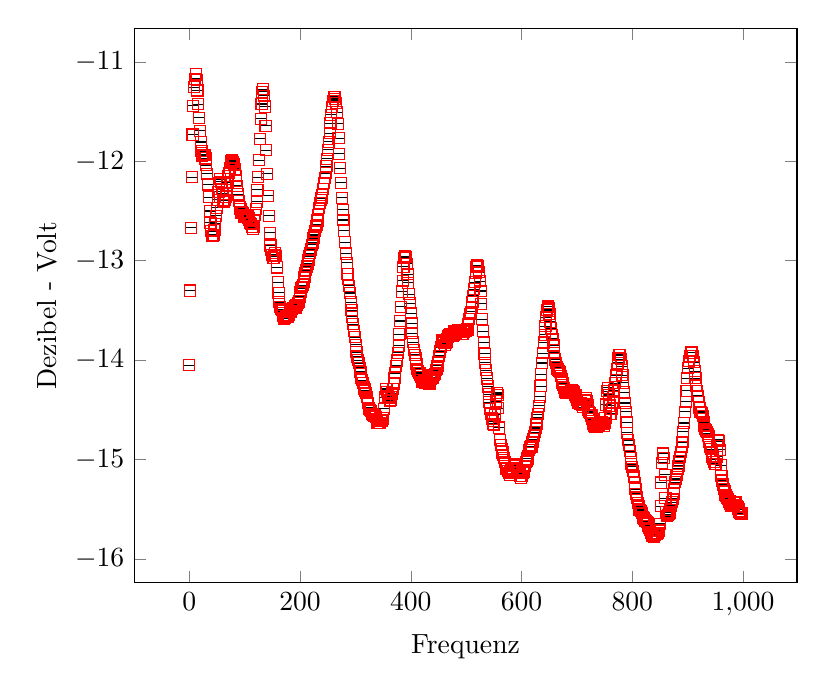
\begin{tikzpicture}
		\pgfplotsset{width=10cm,legend style={font=\footnotesize}}
		\begin{axis}[xlabel={Frequenz},ylabel={Dezibel - Volt},legend cell align=left,legend pos=north west]
		\addplot+[only marks,color=red,mark=square,error bars/.cd,x dir=both,x explicit,y dir=both,y explicit,error bar style={color=black}] table[x=X,y=Y,x error=xerror,y error=yerror,row sep=\\]{
			X	Y	xerror	yerror	\\
			0.0	-14.050505	0	0	\\
			1.464844	-13.299937	0	0	\\
			2.929687	-12.667614	0	0	\\
			4.394531	-12.158621	0	0	\\
			5.859375	-11.730596	0	0	\\
			7.324219	-11.439429	0	0	\\
			8.789062	-11.255181	0	0	\\
			10.253906	-11.167565	0	0	\\
			11.71875	-11.125702	0	0	\\
			13.183594	-11.185375	0	0	\\
			14.648437	-11.286533	0	0	\\
			16.113281	-11.424848	0	0	\\
			17.578125	-11.562135	0	0	\\
			19.042969	-11.692611	0	0	\\
			20.507812	-11.805825	0	0	\\
			21.972656	-11.897202	0	0	\\
			23.4375	-11.942884	0	0	\\
			24.902344	-11.933558	0	0	\\
			26.367187	-11.933213	0	0	\\
			27.832031	-11.935169	0	0	\\
			29.296875	-11.970685	0	0	\\
			30.761719	-12.03641	0	0	\\
			32.226562	-12.12475	0	0	\\
			33.691406	-12.233002	0	0	\\
			35.15625	-12.362489	0	0	\\
			36.621094	-12.499766	0	0	\\
			38.085937	-12.616361	0	0	\\
			39.550781	-12.703513	0	0	\\
			41.015625	-12.752819	0	0	\\
			42.480469	-12.748154	0	0	\\
			43.945312	-12.73773	0	0	\\
			45.410156	-12.692056	0	0	\\
			46.875	-12.627846	0	0	\\
			48.339844	-12.546045	0	0	\\
			49.804687	-12.465853	0	0	\\
			51.269531	-12.387216	0	0	\\
			52.734375	-12.307693	0	0	\\
			54.199219	-12.223723	0	0	\\
			55.664062	-12.177003	0	0	\\
			57.128906	-12.203774	0	0	\\
			58.59375	-12.277561	0	0	\\
			60.058594	-12.328262	0	0	\\
			61.523437	-12.396147	0	0	\\
			62.988281	-12.410666	0	0	\\
			64.453125	-12.386562	0	0	\\
			65.917969	-12.354418	0	0	\\
			67.382812	-12.29202	0	0	\\
			68.847656	-12.212931	0	0	\\
			70.3125	-12.149613	0	0	\\
			71.777344	-12.118436	0	0	\\
			73.242187	-12.069843	0	0	\\
			74.707031	-12.020032	0	0	\\
			76.171875	-11.994096	0	0	\\
			77.636719	-11.985539	0	0	\\
			79.101562	-12.006559	0	0	\\
			80.566406	-12.031732	0	0	\\
			82.03125	-12.072989	0	0	\\
			83.496094	-12.143531	0	0	\\
			84.960937	-12.194586	0	0	\\
			86.425781	-12.247041	0	0	\\
			87.890625	-12.333256	0	0	\\
			89.355469	-12.397348	0	0	\\
			90.820312	-12.458001	0	0	\\
			92.285156	-12.479244	0	0	\\
			93.75	-12.519968	0	0	\\
			95.214844	-12.511867	0	0	\\
			96.679687	-12.51593	0	0	\\
			98.144531	-12.543087	0	0	\\
			99.609375	-12.555055	0	0	\\
			101.074219	-12.546762	0	0	\\
			102.539062	-12.546863	0	0	\\
			104.003906	-12.555903	0	0	\\
			105.46875	-12.550551	0	0	\\
			106.933594	-12.566872	0	0	\\
			108.398437	-12.584899	0	0	\\
			109.863281	-12.619747	0	0	\\
			111.328125	-12.628088	0	0	\\
			112.792969	-12.660742	0	0	\\
			114.257812	-12.683404	0	0	\\
			115.722656	-12.657223	0	0	\\
			117.1875	-12.598691	0	0	\\
			118.652344	-12.537689	0	0	\\
			120.117187	-12.48002	0	0	\\
			121.582031	-12.406897	0	0	\\
			123.046875	-12.28631	0	0	\\
			124.511719	-12.161429	0	0	\\
			125.976562	-11.990362	0	0	\\
			127.441406	-11.771233	0	0	\\
			128.90625	-11.571997	0	0	\\
			130.371094	-11.422843	0	0	\\
			131.835937	-11.299549	0	0	\\
			133.300781	-11.275164	0	0	\\
			134.765625	-11.341789	0	0	\\
			136.230469	-11.44871	0	0	\\
			137.695312	-11.641409	0	0	\\
			139.160156	-11.889627	0	0	\\
			140.625	-12.125895	0	0	\\
			142.089844	-12.345694	0	0	\\
			143.554687	-12.548676	0	0	\\
			145.019531	-12.719376	0	0	\\
			146.484375	-12.846957	0	0	\\
			147.949219	-12.888508	0	0	\\
			149.414062	-12.94263	0	0	\\
			150.878906	-12.973352	0	0	\\
			152.34375	-12.972911	0	0	\\
			153.808594	-12.946934	0	0	\\
			155.273437	-12.918748	0	0	\\
			156.738281	-12.955085	0	0	\\
			158.203125	-13.067271	0	0	\\
			159.667969	-13.216498	0	0	\\
			161.132812	-13.32257	0	0	\\
			162.597656	-13.415944	0	0	\\
			164.0625	-13.466877	0	0	\\
			165.527344	-13.488856	0	0	\\
			166.992187	-13.493699	0	0	\\
			168.457031	-13.509316	0	0	\\
			169.921875	-13.556178	0	0	\\
			171.386719	-13.580522	0	0	\\
			172.851562	-13.573926	0	0	\\
			174.316406	-13.561218	0	0	\\
			175.78125	-13.558925	0	0	\\
			177.246094	-13.560324	0	0	\\
			178.710937	-13.56292	0	0	\\
			180.175781	-13.545437	0	0	\\
			181.640625	-13.517522	0	0	\\
			183.105469	-13.509958	0	0	\\
			184.570312	-13.486111	0	0	\\
			186.035156	-13.4824	0	0	\\
			187.5	-13.479368	0	0	\\
			188.964844	-13.472779	0	0	\\
			190.429687	-13.460141	0	0	\\
			191.894531	-13.469727	0	0	\\
			193.359375	-13.44579	0	0	\\
			194.824219	-13.444059	0	0	\\
			196.289062	-13.42621	0	0	\\
			197.753906	-13.409402	0	0	\\
			199.21875	-13.362461	0	0	\\
			200.683594	-13.314831	0	0	\\
			202.148437	-13.274704	0	0	\\
			203.613281	-13.263993	0	0	\\
			205.078125	-13.246126	0	0	\\
			206.542969	-13.209223	0	0	\\
			208.007812	-13.162423	0	0	\\
			209.472656	-13.119143	0	0	\\
			210.9375	-13.09283	0	0	\\
			212.402344	-13.058518	0	0	\\
			213.867187	-13.032045	0	0	\\
			215.332031	-12.995536	0	0	\\
			216.796875	-12.953788	0	0	\\
			218.261719	-12.923639	0	0	\\
			219.726562	-12.886046	0	0	\\
			221.191406	-12.838865	0	0	\\
			222.65625	-12.819288	0	0	\\
			224.121094	-12.773106	0	0	\\
			225.585937	-12.740998	0	0	\\
			227.050781	-12.696878	0	0	\\
			228.515625	-12.655263	0	0	\\
			229.980469	-12.636984	0	0	\\
			231.445312	-12.59561	0	0	\\
			232.910156	-12.536112	0	0	\\
			234.375	-12.473359	0	0	\\
			235.839844	-12.415836	0	0	\\
			237.304687	-12.390182	0	0	\\
			238.769531	-12.369233	0	0	\\
			240.234375	-12.336422	0	0	\\
			241.699219	-12.280003	0	0	\\
			243.164062	-12.221002	0	0	\\
			244.628906	-12.170596	0	0	\\
			246.09375	-12.119882	0	0	\\
			247.558594	-12.050278	0	0	\\
			249.023437	-11.97433	0	0	\\
			250.488281	-11.884071	0	0	\\
			251.953125	-11.801957	0	0	\\
			253.417969	-11.715909	0	0	\\
			254.882812	-11.615192	0	0	\\
			256.347656	-11.531232	0	0	\\
			257.8125	-11.450738	0	0	\\
			259.277344	-11.391323	0	0	\\
			260.742187	-11.35611	0	0	\\
			262.207031	-11.349498	0	0	\\
			263.671875	-11.372311	0	0	\\
			265.136719	-11.411729	0	0	\\
			266.601562	-11.506046	0	0	\\
			268.066406	-11.621456	0	0	\\
			269.53125	-11.767096	0	0	\\
			270.996094	-11.922912	0	0	\\
			272.460937	-12.070072	0	0	\\
			273.925781	-12.213813	0	0	\\
			275.390625	-12.365535	0	0	\\
			276.855469	-12.488526	0	0	\\
			278.320312	-12.589865	0	0	\\
			279.785156	-12.696111	0	0	\\
			281.25	-12.813684	0	0	\\
			282.714844	-12.927304	0	0	\\
			284.179687	-13.021632	0	0	\\
			285.644531	-13.131017	0	0	\\
			287.109375	-13.186065	0	0	\\
			288.574219	-13.250932	0	0	\\
			290.039062	-13.323876	0	0	\\
			291.503906	-13.419504	0	0	\\
			292.96875	-13.499429	0	0	\\
			294.433594	-13.562529	0	0	\\
			295.898437	-13.637796	0	0	\\
			297.363281	-13.707288	0	0	\\
			298.828125	-13.769209	0	0	\\
			300.292969	-13.846533	0	0	\\
			301.757812	-13.917909	0	0	\\
			303.222656	-13.965913	0	0	\\
			304.6875	-14.002488	0	0	\\
			306.152344	-14.031927	0	0	\\
			307.617187	-14.0776	0	0	\\
			309.082031	-14.119358	0	0	\\
			310.546875	-14.177657	0	0	\\
			312.011719	-14.202594	0	0	\\
			313.476562	-14.233382	0	0	\\
			314.941406	-14.275084	0	0	\\
			316.40625	-14.286332	0	0	\\
			317.871094	-14.305431	0	0	\\
			319.335937	-14.329957	0	0	\\
			320.800781	-14.372081	0	0	\\
			322.265625	-14.431703	0	0	\\
			323.730469	-14.479415	0	0	\\
			325.195312	-14.488866	0	0	\\
			326.660156	-14.504204	0	0	\\
			328.125	-14.513373	0	0	\\
			329.589844	-14.545465	0	0	\\
			331.054687	-14.551137	0	0	\\
			332.519531	-14.554262	0	0	\\
			333.984375	-14.560821	0	0	\\
			335.449219	-14.557158	0	0	\\
			336.914062	-14.57582	0	0	\\
			338.378906	-14.606307	0	0	\\
			339.84375	-14.633411	0	0	\\
			341.308594	-14.628931	0	0	\\
			342.773437	-14.635881	0	0	\\
			344.238281	-14.62858	0	0	\\
			345.703125	-14.605059	0	0	\\
			347.167969	-14.611538	0	0	\\
			348.632812	-14.608422	0	0	\\
			350.097656	-14.586239	0	0	\\
			351.5625	-14.488962	0	0	\\
			353.027344	-14.371365	0	0	\\
			354.492187	-14.290249	0	0	\\
			355.957031	-14.290229	0	0	\\
			357.421875	-14.320078	0	0	\\
			358.886719	-14.358496	0	0	\\
			360.351562	-14.382988	0	0	\\
			361.816406	-14.406957	0	0	\\
			363.28125	-14.398909	0	0	\\
			364.746094	-14.367863	0	0	\\
			366.210937	-14.335484	0	0	\\
			367.675781	-14.29155	0	0	\\
			369.140625	-14.235703	0	0	\\
			370.605469	-14.179809	0	0	\\
			372.070312	-14.129939	0	0	\\
			373.535156	-14.057932	0	0	\\
			375.0	-14.004341	0	0	\\
			376.464844	-13.924224	0	0	\\
			377.929687	-13.855575	0	0	\\
			379.394531	-13.738273	0	0	\\
			380.859375	-13.605998	0	0	\\
			382.324219	-13.464516	0	0	\\
			383.789062	-13.309787	0	0	\\
			385.253906	-13.200063	0	0	\\
			386.71875	-13.060897	0	0	\\
			388.183594	-12.97622	0	0	\\
			389.648437	-12.956916	0	0	\\
			391.113281	-12.965539	0	0	\\
			392.578125	-13.030482	0	0	\\
			394.042969	-13.1343	0	0	\\
			395.507812	-13.22321	0	0	\\
			396.972656	-13.335253	0	0	\\
			398.4375	-13.428647	0	0	\\
			399.902344	-13.529227	0	0	\\
			401.367187	-13.62814	0	0	\\
			402.832031	-13.727482	0	0	\\
			404.296875	-13.819466	0	0	\\
			405.761719	-13.896711	0	0	\\
			407.226562	-13.944845	0	0	\\
			408.691406	-13.982526	0	0	\\
			410.15625	-14.041802	0	0	\\
			411.621094	-14.085652	0	0	\\
			413.085937	-14.111029	0	0	\\
			414.550781	-14.128493	0	0	\\
			416.015625	-14.133768	0	0	\\
			417.480469	-14.151043	0	0	\\
			418.945312	-14.170855	0	0	\\
			420.410156	-14.216436	0	0	\\
			421.875	-14.217036	0	0	\\
			423.339844	-14.210892	0	0	\\
			424.804687	-14.21458	0	0	\\
			426.269531	-14.225149	0	0	\\
			427.734375	-14.225299	0	0	\\
			429.199219	-14.223484	0	0	\\
			430.664062	-14.23328	0	0	\\
			432.128906	-14.242844	0	0	\\
			433.59375	-14.238656	0	0	\\
			435.058594	-14.195949	0	0	\\
			436.523437	-14.18551	0	0	\\
			437.988281	-14.178383	0	0	\\
			439.453125	-14.177931	0	0	\\
			440.917969	-14.15285	0	0	\\
			442.382812	-14.147003	0	0	\\
			443.847656	-14.135528	0	0	\\
			445.3125	-14.102925	0	0	\\
			446.777344	-14.083479	0	0	\\
			448.242187	-14.057502	0	0	\\
			449.707031	-14.018939	0	0	\\
			451.171875	-13.958109	0	0	\\
			452.636719	-13.912992	0	0	\\
			454.101562	-13.87162	0	0	\\
			455.566406	-13.80972	0	0	\\
			457.03125	-13.802168	0	0	\\
			458.496094	-13.814805	0	0	\\
			459.960937	-13.828085	0	0	\\
			461.425781	-13.843606	0	0	\\
			462.890625	-13.825697	0	0	\\
			464.355469	-13.815212	0	0	\\
			465.820312	-13.78755	0	0	\\
			467.285156	-13.76159	0	0	\\
			468.75	-13.750413	0	0	\\
			470.214844	-13.749508	0	0	\\
			471.679687	-13.739326	0	0	\\
			473.144531	-13.73774	0	0	\\
			474.609375	-13.741617	0	0	\\
			476.074219	-13.756798	0	0	\\
			477.539062	-13.743379	0	0	\\
			479.003906	-13.711689	0	0	\\
			480.46875	-13.715047	0	0	\\
			481.933594	-13.730951	0	0	\\
			483.398437	-13.720465	0	0	\\
			484.863281	-13.696815	0	0	\\
			486.328125	-13.714307	0	0	\\
			487.792969	-13.712178	0	0	\\
			489.257812	-13.715804	0	0	\\
			490.722656	-13.717373	0	0	\\
			492.1875	-13.733816	0	0	\\
			493.652344	-13.7371	0	0	\\
			495.117187	-13.716919	0	0	\\
			496.582031	-13.704679	0	0	\\
			498.046875	-13.707767	0	0	\\
			499.511719	-13.706872	0	0	\\
			500.976562	-13.685887	0	0	\\
			502.441406	-13.691197	0	0	\\
			503.90625	-13.64209	0	0	\\
			505.371094	-13.58796	0	0	\\
			506.835937	-13.535002	0	0	\\
			508.300781	-13.513402	0	0	\\
			509.765625	-13.478852	0	0	\\
			511.230469	-13.412173	0	0	\\
			512.695312	-13.350785	0	0	\\
			514.160156	-13.286017	0	0	\\
			515.625	-13.216078	0	0	\\
			517.089844	-13.119241	0	0	\\
			518.554687	-13.065301	0	0	\\
			520.019531	-13.047169	0	0	\\
			521.484375	-13.05185	0	0	\\
			522.949219	-13.114488	0	0	\\
			524.414062	-13.204968	0	0	\\
			525.878906	-13.304042	0	0	\\
			527.34375	-13.4332	0	0	\\
			528.808594	-13.587725	0	0	\\
			530.273437	-13.707911	0	0	\\
			531.738281	-13.822526	0	0	\\
			533.203125	-13.936431	0	0	\\
			534.667969	-14.026417	0	0	\\
			536.132812	-14.102635	0	0	\\
			537.597656	-14.184221	0	0	\\
			539.0625	-14.264295	0	0	\\
			540.527344	-14.341433	0	0	\\
			541.992187	-14.422495	0	0	\\
			543.457031	-14.48791	0	0	\\
			544.921875	-14.536511	0	0	\\
			546.386719	-14.587397	0	0	\\
			547.851562	-14.612427	0	0	\\
			549.316406	-14.641665	0	0	\\
			550.78125	-14.647993	0	0	\\
			552.246094	-14.546999	0	0	\\
			553.710937	-14.415276	0	0	\\
			555.175781	-14.330225	0	0	\\
			556.640625	-14.350996	0	0	\\
			558.105469	-14.482412	0	0	\\
			559.570312	-14.677802	0	0	\\
			561.035156	-14.800089	0	0	\\
			562.5	-14.85551	0	0	\\
			563.964844	-14.894614	0	0	\\
			565.429687	-14.928676	0	0	\\
			566.894531	-14.952805	0	0	\\
			568.359375	-14.98422	0	0	\\
			569.824219	-15.028166	0	0	\\
			571.289062	-15.083012	0	0	\\
			572.753906	-15.090926	0	0	\\
			574.21875	-15.094026	0	0	\\
			575.683594	-15.114998	0	0	\\
			577.148437	-15.136628	0	0	\\
			578.613281	-15.15258	0	0	\\
			580.078125	-15.122533	0	0	\\
			581.542969	-15.107289	0	0	\\
			583.007812	-15.094602	0	0	\\
			584.472656	-15.082529	0	0	\\
			585.9375	-15.059935	0	0	\\
			587.402344	-15.058453	0	0	\\
			588.867187	-15.046029	0	0	\\
			590.332031	-15.06678	0	0	\\
			591.796875	-15.099119	0	0	\\
			593.261719	-15.135108	0	0	\\
			594.726562	-15.128433	0	0	\\
			596.191406	-15.137806	0	0	\\
			597.65625	-15.166473	0	0	\\
			599.121094	-15.180882	0	0	\\
			600.585937	-15.163743	0	0	\\
			602.050781	-15.133186	0	0	\\
			603.515625	-15.125595	0	0	\\
			604.980469	-15.115409	0	0	\\
			606.445312	-15.067269	0	0	\\
			607.910156	-15.023027	0	0	\\
			609.375	-15.009752	0	0	\\
			610.839844	-14.989937	0	0	\\
			612.304687	-14.967128	0	0	\\
			613.769531	-14.905996	0	0	\\
			615.234375	-14.878592	0	0	\\
			616.699219	-14.866289	0	0	\\
			618.164062	-14.868215	0	0	\\
			619.628906	-14.822102	0	0	\\
			621.09375	-14.793859	0	0	\\
			622.558594	-14.766284	0	0	\\
			624.023437	-14.725277	0	0	\\
			625.488281	-14.682154	0	0	\\
			626.953125	-14.640055	0	0	\\
			628.417969	-14.581117	0	0	\\
			629.882812	-14.545271	0	0	\\
			631.347656	-14.459573	0	0	\\
			632.8125	-14.366694	0	0	\\
			634.277344	-14.263101	0	0	\\
			635.742187	-14.142677	0	0	\\
			637.207031	-14.028242	0	0	\\
			638.671875	-13.931155	0	0	\\
			640.136719	-13.822631	0	0	\\
			641.601562	-13.745261	0	0	\\
			643.066406	-13.658316	0	0	\\
			644.53125	-13.569186	0	0	\\
			645.996094	-13.495608	0	0	\\
			647.460937	-13.46108	0	0	\\
			648.925781	-13.480555	0	0	\\
			650.390625	-13.538272	0	0	\\
			651.855469	-13.613028	0	0	\\
			653.320312	-13.681032	0	0	\\
			654.785156	-13.744338	0	0	\\
			656.25	-13.784262	0	0	\\
			657.714844	-13.851768	0	0	\\
			659.179687	-13.924064	0	0	\\
			660.644531	-13.993007	0	0	\\
			662.109375	-14.025634	0	0	\\
			663.574219	-14.069885	0	0	\\
			665.039062	-14.087395	0	0	\\
			666.503906	-14.10298	0	0	\\
			667.96875	-14.1068	0	0	\\
			669.433594	-14.122748	0	0	\\
			670.898437	-14.162633	0	0	\\
			672.363281	-14.192739	0	0	\\
			673.828125	-14.230496	0	0	\\
			675.292969	-14.247783	0	0	\\
			676.757812	-14.283354	0	0	\\
			678.222656	-14.316979	0	0	\\
			679.6875	-14.33117	0	0	\\
			681.152344	-14.326027	0	0	\\
			682.617187	-14.322572	0	0	\\
			684.082031	-14.322422	0	0	\\
			685.546875	-14.318143	0	0	\\
			687.011719	-14.32596	0	0	\\
			688.476562	-14.322964	0	0	\\
			689.941406	-14.308299	0	0	\\
			691.40625	-14.298386	0	0	\\
			692.871094	-14.307418	0	0	\\
			694.335937	-14.324684	0	0	\\
			695.800781	-14.351422	0	0	\\
			697.265625	-14.352408	0	0	\\
			698.730469	-14.36568	0	0	\\
			700.195312	-14.404201	0	0	\\
			701.660156	-14.430898	0	0	\\
			703.125	-14.427039	0	0	\\
			704.589844	-14.434381	0	0	\\
			706.054687	-14.435618	0	0	\\
			707.519531	-14.432911	0	0	\\
			708.984375	-14.446435	0	0	\\
			710.449219	-14.475005	0	0	\\
			711.914062	-14.452262	0	0	\\
			713.378906	-14.437378	0	0	\\
			714.84375	-14.404899	0	0	\\
			716.308594	-14.385541	0	0	\\
			717.773437	-14.415438	0	0	\\
			719.238281	-14.454149	0	0	\\
			720.703125	-14.497398	0	0	\\
			722.167969	-14.520317	0	0	\\
			723.632812	-14.529866	0	0	\\
			725.097656	-14.557658	0	0	\\
			726.5625	-14.555079	0	0	\\
			728.027344	-14.596049	0	0	\\
			729.492187	-14.638483	0	0	\\
			730.957031	-14.66205	0	0	\\
			732.421875	-14.675452	0	0	\\
			733.886719	-14.675422	0	0	\\
			735.351562	-14.672214	0	0	\\
			736.816406	-14.656058	0	0	\\
			738.28125	-14.651118	0	0	\\
			739.746094	-14.649747	0	0	\\
			741.210937	-14.636523	0	0	\\
			742.675781	-14.636155	0	0	\\
			744.140625	-14.6218	0	0	\\
			745.605469	-14.625461	0	0	\\
			747.070312	-14.643622	0	0	\\
			748.535156	-14.657819	0	0	\\
			750.0	-14.631515	0	0	\\
			751.464844	-14.582607	0	0	\\
			752.929687	-14.446605	0	0	\\
			754.394531	-14.312882	0	0	\\
			755.859375	-14.276123	0	0	\\
			757.324219	-14.350377	0	0	\\
			758.789062	-14.456408	0	0	\\
			760.253906	-14.541881	0	0	\\
			761.71875	-14.537256	0	0	\\
			763.183594	-14.488729	0	0	\\
			764.648437	-14.427315	0	0	\\
			766.113281	-14.37244	0	0	\\
			767.578125	-14.305331	0	0	\\
			769.042969	-14.232469	0	0	\\
			770.507812	-14.155074	0	0	\\
			771.972656	-14.091079	0	0	\\
			773.4375	-14.027252	0	0	\\
			774.902344	-13.975445	0	0	\\
			776.367187	-13.949346	0	0	\\
			777.832031	-13.947627	0	0	\\
			779.296875	-13.991495	0	0	\\
			780.761719	-14.061561	0	0	\\
			782.226562	-14.150668	0	0	\\
			783.691406	-14.228971	0	0	\\
			785.15625	-14.324549	0	0	\\
			786.621094	-14.430608	0	0	\\
			788.085937	-14.51929	0	0	\\
			789.550781	-14.623041	0	0	\\
			791.015625	-14.730229	0	0	\\
			792.480469	-14.805449	0	0	\\
			793.945312	-14.852743	0	0	\\
			795.410156	-14.914466	0	0	\\
			796.875	-14.986443	0	0	\\
			798.339844	-15.047592	0	0	\\
			799.804687	-15.071631	0	0	\\
			801.269531	-15.114165	0	0	\\
			802.734375	-15.170488	0	0	\\
			804.199219	-15.239781	0	0	\\
			805.664062	-15.295695	0	0	\\
			807.128906	-15.346834	0	0	\\
			808.59375	-15.382291	0	0	\\
			810.058594	-15.438962	0	0	\\
			811.523437	-15.472461	0	0	\\
			812.988281	-15.505756	0	0	\\
			814.453125	-15.51089	0	0	\\
			815.917969	-15.516134	0	0	\\
			817.382812	-15.538309	0	0	\\
			818.847656	-15.577786	0	0	\\
			820.3125	-15.590476	0	0	\\
			821.777344	-15.592755	0	0	\\
			823.242187	-15.613741	0	0	\\
			824.707031	-15.614099	0	0	\\
			826.171875	-15.625513	0	0	\\
			827.636719	-15.638591	0	0	\\
			829.101562	-15.667989	0	0	\\
			830.566406	-15.689446	0	0	\\
			832.03125	-15.711343	0	0	\\
			833.496094	-15.735803	0	0	\\
			834.960937	-15.748217	0	0	\\
			836.425781	-15.766733	0	0	\\
			837.890625	-15.762721	0	0	\\
			839.355469	-15.775128	0	0	\\
			840.820312	-15.754851	0	0	\\
			842.285156	-15.745726	0	0	\\
			843.75	-15.746132	0	0	\\
			845.214844	-15.740792	0	0	\\
			846.679687	-15.737162	0	0	\\
			848.144531	-15.713806	0	0	\\
			849.609375	-15.648701	0	0	\\
			851.074219	-15.469149	0	0	\\
			852.539062	-15.231399	0	0	\\
			854.003906	-15.031341	0	0	\\
			855.46875	-14.939818	0	0	\\
			856.933594	-14.982826	0	0	\\
			858.398437	-15.151275	0	0	\\
			859.863281	-15.387465	0	0	\\
			861.328125	-15.525493	0	0	\\
			862.792969	-15.567574	0	0	\\
			864.257812	-15.55716	0	0	\\
			865.722656	-15.548389	0	0	\\
			867.1875	-15.531781	0	0	\\
			868.652344	-15.507071	0	0	\\
			870.117187	-15.465653	0	0	\\
			871.582031	-15.428138	0	0	\\
			873.046875	-15.396552	0	0	\\
			874.511719	-15.348787	0	0	\\
			875.976562	-15.293764	0	0	\\
			877.441406	-15.22911	0	0	\\
			878.90625	-15.195975	0	0	\\
			880.371094	-15.153742	0	0	\\
			881.835937	-15.092107	0	0	\\
			883.300781	-15.062193	0	0	\\
			884.765625	-15.016929	0	0	\\
			886.230469	-14.972279	0	0	\\
			887.695312	-14.925672	0	0	\\
			889.160156	-14.876122	0	0	\\
			890.625	-14.823821	0	0	\\
			892.089844	-14.721841	0	0	\\
			893.554687	-14.631986	0	0	\\
			895.019531	-14.519774	0	0	\\
			896.484375	-14.418282	0	0	\\
			897.949219	-14.308576	0	0	\\
			899.414062	-14.181744	0	0	\\
			900.878906	-14.079504	0	0	\\
			902.34375	-14.009096	0	0	\\
			903.808594	-13.95814	0	0	\\
			905.273437	-13.9262	0	0	\\
			906.738281	-13.923177	0	0	\\
			908.203125	-13.923957	0	0	\\
			909.667969	-13.960398	0	0	\\
			911.132812	-14.021155	0	0	\\
			912.597656	-14.111932	0	0	\\
			914.0625	-14.180354	0	0	\\
			915.527344	-14.255244	0	0	\\
			916.992187	-14.309459	0	0	\\
			918.457031	-14.359127	0	0	\\
			919.921875	-14.424297	0	0	\\
			921.386719	-14.477953	0	0	\\
			922.851562	-14.520959	0	0	\\
			924.316406	-14.525141	0	0	\\
			925.78125	-14.531666	0	0	\\
			927.246094	-14.565809	0	0	\\
			928.710937	-14.625074	0	0	\\
			930.175781	-14.658041	0	0	\\
			931.640625	-14.69385	0	0	\\
			933.105469	-14.708211	0	0	\\
			934.570312	-14.722134	0	0	\\
			936.035156	-14.739455	0	0	\\
			937.5	-14.760567	0	0	\\
			938.964844	-14.818323	0	0	\\
			940.429687	-14.870238	0	0	\\
			941.894531	-14.895099	0	0	\\
			943.359375	-14.929479	0	0	\\
			944.824219	-14.969275	0	0	\\
			946.289062	-14.994583	0	0	\\
			947.753906	-15.021683	0	0	\\
			949.21875	-15.047419	0	0	\\
			950.683594	-15.04475	0	0	\\
			952.148437	-14.970457	0	0	\\
			953.613281	-14.866085	0	0	\\
			955.078125	-14.799097	0	0	\\
			956.542969	-14.815702	0	0	\\
			958.007812	-14.901837	0	0	\\
			959.472656	-15.057832	0	0	\\
			960.9375	-15.162472	0	0	\\
			962.402344	-15.21057	0	0	\\
			963.867187	-15.250887	0	0	\\
			965.332031	-15.297959	0	0	\\
			966.796875	-15.320597	0	0	\\
			968.261719	-15.355816	0	0	\\
			969.726562	-15.367667	0	0	\\
			971.191406	-15.382371	0	0	\\
			972.65625	-15.395509	0	0	\\
			974.121094	-15.422016	0	0	\\
			975.585937	-15.420453	0	0	\\
			977.050781	-15.441803	0	0	\\
			978.515625	-15.462805	0	0	\\
			979.980469	-15.46989	0	0	\\
			981.445312	-15.467675	0	0	\\
			982.910156	-15.459868	0	0	\\
			984.375	-15.437176	0	0	\\
			985.839844	-15.428645	0	0	\\
			987.304687	-15.429379	0	0	\\
			988.769531	-15.463354	0	0	\\
			990.234375	-15.476478	0	0	\\
			991.699219	-15.500575	0	0	\\
			993.164062	-15.521667	0	0	\\
			994.628906	-15.539474	0	0	\\
			996.09375	-15.54427	0	0	\\
			997.558594	-15.541833	0	0	\\
		};		% \addlegendentry{Messpunkte Datensatz 0}
		\end{axis}
		\end{tikzpicture}
	\caption{$T=0\si\degree$}
	\label{fig:Umgebungsmessung}
\end{figure}
            \begin{figure}[H]
	\centering
	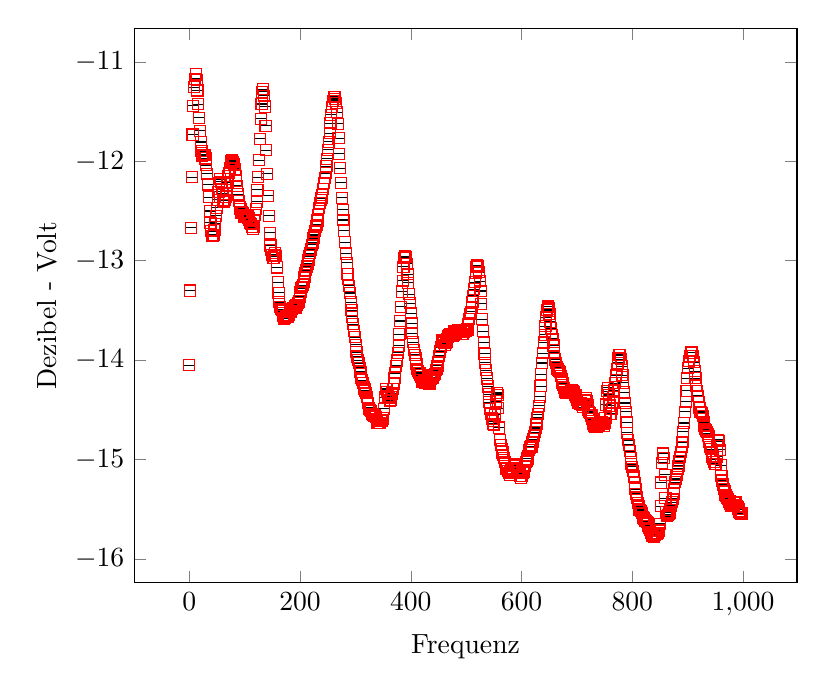
\begin{tikzpicture}
		\pgfplotsset{width=10cm,legend style={font=\footnotesize}}
		\begin{axis}[xlabel={Frequenz},ylabel={Dezibel - Volt},legend cell align=left,legend pos=north west]
		\addplot+[only marks,color=red,mark=square,error bars/.cd,x dir=both,x explicit,y dir=both,y explicit,error bar style={color=black}] table[x=X,y=Y,x error=xerror,y error=yerror,row sep=\\]{
			X	Y	xerror	yerror	\\
			0.0	-14.050505	0	0	\\
			1.464844	-13.299937	0	0	\\
			2.929687	-12.667614	0	0	\\
			4.394531	-12.158621	0	0	\\
			5.859375	-11.730596	0	0	\\
			7.324219	-11.439429	0	0	\\
			8.789062	-11.255181	0	0	\\
			10.253906	-11.167565	0	0	\\
			11.71875	-11.125702	0	0	\\
			13.183594	-11.185375	0	0	\\
			14.648437	-11.286533	0	0	\\
			16.113281	-11.424848	0	0	\\
			17.578125	-11.562135	0	0	\\
			19.042969	-11.692611	0	0	\\
			20.507812	-11.805825	0	0	\\
			21.972656	-11.897202	0	0	\\
			23.4375	-11.942884	0	0	\\
			24.902344	-11.933558	0	0	\\
			26.367187	-11.933213	0	0	\\
			27.832031	-11.935169	0	0	\\
			29.296875	-11.970685	0	0	\\
			30.761719	-12.03641	0	0	\\
			32.226562	-12.12475	0	0	\\
			33.691406	-12.233002	0	0	\\
			35.15625	-12.362489	0	0	\\
			36.621094	-12.499766	0	0	\\
			38.085937	-12.616361	0	0	\\
			39.550781	-12.703513	0	0	\\
			41.015625	-12.752819	0	0	\\
			42.480469	-12.748154	0	0	\\
			43.945312	-12.73773	0	0	\\
			45.410156	-12.692056	0	0	\\
			46.875	-12.627846	0	0	\\
			48.339844	-12.546045	0	0	\\
			49.804687	-12.465853	0	0	\\
			51.269531	-12.387216	0	0	\\
			52.734375	-12.307693	0	0	\\
			54.199219	-12.223723	0	0	\\
			55.664062	-12.177003	0	0	\\
			57.128906	-12.203774	0	0	\\
			58.59375	-12.277561	0	0	\\
			60.058594	-12.328262	0	0	\\
			61.523437	-12.396147	0	0	\\
			62.988281	-12.410666	0	0	\\
			64.453125	-12.386562	0	0	\\
			65.917969	-12.354418	0	0	\\
			67.382812	-12.29202	0	0	\\
			68.847656	-12.212931	0	0	\\
			70.3125	-12.149613	0	0	\\
			71.777344	-12.118436	0	0	\\
			73.242187	-12.069843	0	0	\\
			74.707031	-12.020032	0	0	\\
			76.171875	-11.994096	0	0	\\
			77.636719	-11.985539	0	0	\\
			79.101562	-12.006559	0	0	\\
			80.566406	-12.031732	0	0	\\
			82.03125	-12.072989	0	0	\\
			83.496094	-12.143531	0	0	\\
			84.960937	-12.194586	0	0	\\
			86.425781	-12.247041	0	0	\\
			87.890625	-12.333256	0	0	\\
			89.355469	-12.397348	0	0	\\
			90.820312	-12.458001	0	0	\\
			92.285156	-12.479244	0	0	\\
			93.75	-12.519968	0	0	\\
			95.214844	-12.511867	0	0	\\
			96.679687	-12.51593	0	0	\\
			98.144531	-12.543087	0	0	\\
			99.609375	-12.555055	0	0	\\
			101.074219	-12.546762	0	0	\\
			102.539062	-12.546863	0	0	\\
			104.003906	-12.555903	0	0	\\
			105.46875	-12.550551	0	0	\\
			106.933594	-12.566872	0	0	\\
			108.398437	-12.584899	0	0	\\
			109.863281	-12.619747	0	0	\\
			111.328125	-12.628088	0	0	\\
			112.792969	-12.660742	0	0	\\
			114.257812	-12.683404	0	0	\\
			115.722656	-12.657223	0	0	\\
			117.1875	-12.598691	0	0	\\
			118.652344	-12.537689	0	0	\\
			120.117187	-12.48002	0	0	\\
			121.582031	-12.406897	0	0	\\
			123.046875	-12.28631	0	0	\\
			124.511719	-12.161429	0	0	\\
			125.976562	-11.990362	0	0	\\
			127.441406	-11.771233	0	0	\\
			128.90625	-11.571997	0	0	\\
			130.371094	-11.422843	0	0	\\
			131.835937	-11.299549	0	0	\\
			133.300781	-11.275164	0	0	\\
			134.765625	-11.341789	0	0	\\
			136.230469	-11.44871	0	0	\\
			137.695312	-11.641409	0	0	\\
			139.160156	-11.889627	0	0	\\
			140.625	-12.125895	0	0	\\
			142.089844	-12.345694	0	0	\\
			143.554687	-12.548676	0	0	\\
			145.019531	-12.719376	0	0	\\
			146.484375	-12.846957	0	0	\\
			147.949219	-12.888508	0	0	\\
			149.414062	-12.94263	0	0	\\
			150.878906	-12.973352	0	0	\\
			152.34375	-12.972911	0	0	\\
			153.808594	-12.946934	0	0	\\
			155.273437	-12.918748	0	0	\\
			156.738281	-12.955085	0	0	\\
			158.203125	-13.067271	0	0	\\
			159.667969	-13.216498	0	0	\\
			161.132812	-13.32257	0	0	\\
			162.597656	-13.415944	0	0	\\
			164.0625	-13.466877	0	0	\\
			165.527344	-13.488856	0	0	\\
			166.992187	-13.493699	0	0	\\
			168.457031	-13.509316	0	0	\\
			169.921875	-13.556178	0	0	\\
			171.386719	-13.580522	0	0	\\
			172.851562	-13.573926	0	0	\\
			174.316406	-13.561218	0	0	\\
			175.78125	-13.558925	0	0	\\
			177.246094	-13.560324	0	0	\\
			178.710937	-13.56292	0	0	\\
			180.175781	-13.545437	0	0	\\
			181.640625	-13.517522	0	0	\\
			183.105469	-13.509958	0	0	\\
			184.570312	-13.486111	0	0	\\
			186.035156	-13.4824	0	0	\\
			187.5	-13.479368	0	0	\\
			188.964844	-13.472779	0	0	\\
			190.429687	-13.460141	0	0	\\
			191.894531	-13.469727	0	0	\\
			193.359375	-13.44579	0	0	\\
			194.824219	-13.444059	0	0	\\
			196.289062	-13.42621	0	0	\\
			197.753906	-13.409402	0	0	\\
			199.21875	-13.362461	0	0	\\
			200.683594	-13.314831	0	0	\\
			202.148437	-13.274704	0	0	\\
			203.613281	-13.263993	0	0	\\
			205.078125	-13.246126	0	0	\\
			206.542969	-13.209223	0	0	\\
			208.007812	-13.162423	0	0	\\
			209.472656	-13.119143	0	0	\\
			210.9375	-13.09283	0	0	\\
			212.402344	-13.058518	0	0	\\
			213.867187	-13.032045	0	0	\\
			215.332031	-12.995536	0	0	\\
			216.796875	-12.953788	0	0	\\
			218.261719	-12.923639	0	0	\\
			219.726562	-12.886046	0	0	\\
			221.191406	-12.838865	0	0	\\
			222.65625	-12.819288	0	0	\\
			224.121094	-12.773106	0	0	\\
			225.585937	-12.740998	0	0	\\
			227.050781	-12.696878	0	0	\\
			228.515625	-12.655263	0	0	\\
			229.980469	-12.636984	0	0	\\
			231.445312	-12.59561	0	0	\\
			232.910156	-12.536112	0	0	\\
			234.375	-12.473359	0	0	\\
			235.839844	-12.415836	0	0	\\
			237.304687	-12.390182	0	0	\\
			238.769531	-12.369233	0	0	\\
			240.234375	-12.336422	0	0	\\
			241.699219	-12.280003	0	0	\\
			243.164062	-12.221002	0	0	\\
			244.628906	-12.170596	0	0	\\
			246.09375	-12.119882	0	0	\\
			247.558594	-12.050278	0	0	\\
			249.023437	-11.97433	0	0	\\
			250.488281	-11.884071	0	0	\\
			251.953125	-11.801957	0	0	\\
			253.417969	-11.715909	0	0	\\
			254.882812	-11.615192	0	0	\\
			256.347656	-11.531232	0	0	\\
			257.8125	-11.450738	0	0	\\
			259.277344	-11.391323	0	0	\\
			260.742187	-11.35611	0	0	\\
			262.207031	-11.349498	0	0	\\
			263.671875	-11.372311	0	0	\\
			265.136719	-11.411729	0	0	\\
			266.601562	-11.506046	0	0	\\
			268.066406	-11.621456	0	0	\\
			269.53125	-11.767096	0	0	\\
			270.996094	-11.922912	0	0	\\
			272.460937	-12.070072	0	0	\\
			273.925781	-12.213813	0	0	\\
			275.390625	-12.365535	0	0	\\
			276.855469	-12.488526	0	0	\\
			278.320312	-12.589865	0	0	\\
			279.785156	-12.696111	0	0	\\
			281.25	-12.813684	0	0	\\
			282.714844	-12.927304	0	0	\\
			284.179687	-13.021632	0	0	\\
			285.644531	-13.131017	0	0	\\
			287.109375	-13.186065	0	0	\\
			288.574219	-13.250932	0	0	\\
			290.039062	-13.323876	0	0	\\
			291.503906	-13.419504	0	0	\\
			292.96875	-13.499429	0	0	\\
			294.433594	-13.562529	0	0	\\
			295.898437	-13.637796	0	0	\\
			297.363281	-13.707288	0	0	\\
			298.828125	-13.769209	0	0	\\
			300.292969	-13.846533	0	0	\\
			301.757812	-13.917909	0	0	\\
			303.222656	-13.965913	0	0	\\
			304.6875	-14.002488	0	0	\\
			306.152344	-14.031927	0	0	\\
			307.617187	-14.0776	0	0	\\
			309.082031	-14.119358	0	0	\\
			310.546875	-14.177657	0	0	\\
			312.011719	-14.202594	0	0	\\
			313.476562	-14.233382	0	0	\\
			314.941406	-14.275084	0	0	\\
			316.40625	-14.286332	0	0	\\
			317.871094	-14.305431	0	0	\\
			319.335937	-14.329957	0	0	\\
			320.800781	-14.372081	0	0	\\
			322.265625	-14.431703	0	0	\\
			323.730469	-14.479415	0	0	\\
			325.195312	-14.488866	0	0	\\
			326.660156	-14.504204	0	0	\\
			328.125	-14.513373	0	0	\\
			329.589844	-14.545465	0	0	\\
			331.054687	-14.551137	0	0	\\
			332.519531	-14.554262	0	0	\\
			333.984375	-14.560821	0	0	\\
			335.449219	-14.557158	0	0	\\
			336.914062	-14.57582	0	0	\\
			338.378906	-14.606307	0	0	\\
			339.84375	-14.633411	0	0	\\
			341.308594	-14.628931	0	0	\\
			342.773437	-14.635881	0	0	\\
			344.238281	-14.62858	0	0	\\
			345.703125	-14.605059	0	0	\\
			347.167969	-14.611538	0	0	\\
			348.632812	-14.608422	0	0	\\
			350.097656	-14.586239	0	0	\\
			351.5625	-14.488962	0	0	\\
			353.027344	-14.371365	0	0	\\
			354.492187	-14.290249	0	0	\\
			355.957031	-14.290229	0	0	\\
			357.421875	-14.320078	0	0	\\
			358.886719	-14.358496	0	0	\\
			360.351562	-14.382988	0	0	\\
			361.816406	-14.406957	0	0	\\
			363.28125	-14.398909	0	0	\\
			364.746094	-14.367863	0	0	\\
			366.210937	-14.335484	0	0	\\
			367.675781	-14.29155	0	0	\\
			369.140625	-14.235703	0	0	\\
			370.605469	-14.179809	0	0	\\
			372.070312	-14.129939	0	0	\\
			373.535156	-14.057932	0	0	\\
			375.0	-14.004341	0	0	\\
			376.464844	-13.924224	0	0	\\
			377.929687	-13.855575	0	0	\\
			379.394531	-13.738273	0	0	\\
			380.859375	-13.605998	0	0	\\
			382.324219	-13.464516	0	0	\\
			383.789062	-13.309787	0	0	\\
			385.253906	-13.200063	0	0	\\
			386.71875	-13.060897	0	0	\\
			388.183594	-12.97622	0	0	\\
			389.648437	-12.956916	0	0	\\
			391.113281	-12.965539	0	0	\\
			392.578125	-13.030482	0	0	\\
			394.042969	-13.1343	0	0	\\
			395.507812	-13.22321	0	0	\\
			396.972656	-13.335253	0	0	\\
			398.4375	-13.428647	0	0	\\
			399.902344	-13.529227	0	0	\\
			401.367187	-13.62814	0	0	\\
			402.832031	-13.727482	0	0	\\
			404.296875	-13.819466	0	0	\\
			405.761719	-13.896711	0	0	\\
			407.226562	-13.944845	0	0	\\
			408.691406	-13.982526	0	0	\\
			410.15625	-14.041802	0	0	\\
			411.621094	-14.085652	0	0	\\
			413.085937	-14.111029	0	0	\\
			414.550781	-14.128493	0	0	\\
			416.015625	-14.133768	0	0	\\
			417.480469	-14.151043	0	0	\\
			418.945312	-14.170855	0	0	\\
			420.410156	-14.216436	0	0	\\
			421.875	-14.217036	0	0	\\
			423.339844	-14.210892	0	0	\\
			424.804687	-14.21458	0	0	\\
			426.269531	-14.225149	0	0	\\
			427.734375	-14.225299	0	0	\\
			429.199219	-14.223484	0	0	\\
			430.664062	-14.23328	0	0	\\
			432.128906	-14.242844	0	0	\\
			433.59375	-14.238656	0	0	\\
			435.058594	-14.195949	0	0	\\
			436.523437	-14.18551	0	0	\\
			437.988281	-14.178383	0	0	\\
			439.453125	-14.177931	0	0	\\
			440.917969	-14.15285	0	0	\\
			442.382812	-14.147003	0	0	\\
			443.847656	-14.135528	0	0	\\
			445.3125	-14.102925	0	0	\\
			446.777344	-14.083479	0	0	\\
			448.242187	-14.057502	0	0	\\
			449.707031	-14.018939	0	0	\\
			451.171875	-13.958109	0	0	\\
			452.636719	-13.912992	0	0	\\
			454.101562	-13.87162	0	0	\\
			455.566406	-13.80972	0	0	\\
			457.03125	-13.802168	0	0	\\
			458.496094	-13.814805	0	0	\\
			459.960937	-13.828085	0	0	\\
			461.425781	-13.843606	0	0	\\
			462.890625	-13.825697	0	0	\\
			464.355469	-13.815212	0	0	\\
			465.820312	-13.78755	0	0	\\
			467.285156	-13.76159	0	0	\\
			468.75	-13.750413	0	0	\\
			470.214844	-13.749508	0	0	\\
			471.679687	-13.739326	0	0	\\
			473.144531	-13.73774	0	0	\\
			474.609375	-13.741617	0	0	\\
			476.074219	-13.756798	0	0	\\
			477.539062	-13.743379	0	0	\\
			479.003906	-13.711689	0	0	\\
			480.46875	-13.715047	0	0	\\
			481.933594	-13.730951	0	0	\\
			483.398437	-13.720465	0	0	\\
			484.863281	-13.696815	0	0	\\
			486.328125	-13.714307	0	0	\\
			487.792969	-13.712178	0	0	\\
			489.257812	-13.715804	0	0	\\
			490.722656	-13.717373	0	0	\\
			492.1875	-13.733816	0	0	\\
			493.652344	-13.7371	0	0	\\
			495.117187	-13.716919	0	0	\\
			496.582031	-13.704679	0	0	\\
			498.046875	-13.707767	0	0	\\
			499.511719	-13.706872	0	0	\\
			500.976562	-13.685887	0	0	\\
			502.441406	-13.691197	0	0	\\
			503.90625	-13.64209	0	0	\\
			505.371094	-13.58796	0	0	\\
			506.835937	-13.535002	0	0	\\
			508.300781	-13.513402	0	0	\\
			509.765625	-13.478852	0	0	\\
			511.230469	-13.412173	0	0	\\
			512.695312	-13.350785	0	0	\\
			514.160156	-13.286017	0	0	\\
			515.625	-13.216078	0	0	\\
			517.089844	-13.119241	0	0	\\
			518.554687	-13.065301	0	0	\\
			520.019531	-13.047169	0	0	\\
			521.484375	-13.05185	0	0	\\
			522.949219	-13.114488	0	0	\\
			524.414062	-13.204968	0	0	\\
			525.878906	-13.304042	0	0	\\
			527.34375	-13.4332	0	0	\\
			528.808594	-13.587725	0	0	\\
			530.273437	-13.707911	0	0	\\
			531.738281	-13.822526	0	0	\\
			533.203125	-13.936431	0	0	\\
			534.667969	-14.026417	0	0	\\
			536.132812	-14.102635	0	0	\\
			537.597656	-14.184221	0	0	\\
			539.0625	-14.264295	0	0	\\
			540.527344	-14.341433	0	0	\\
			541.992187	-14.422495	0	0	\\
			543.457031	-14.48791	0	0	\\
			544.921875	-14.536511	0	0	\\
			546.386719	-14.587397	0	0	\\
			547.851562	-14.612427	0	0	\\
			549.316406	-14.641665	0	0	\\
			550.78125	-14.647993	0	0	\\
			552.246094	-14.546999	0	0	\\
			553.710937	-14.415276	0	0	\\
			555.175781	-14.330225	0	0	\\
			556.640625	-14.350996	0	0	\\
			558.105469	-14.482412	0	0	\\
			559.570312	-14.677802	0	0	\\
			561.035156	-14.800089	0	0	\\
			562.5	-14.85551	0	0	\\
			563.964844	-14.894614	0	0	\\
			565.429687	-14.928676	0	0	\\
			566.894531	-14.952805	0	0	\\
			568.359375	-14.98422	0	0	\\
			569.824219	-15.028166	0	0	\\
			571.289062	-15.083012	0	0	\\
			572.753906	-15.090926	0	0	\\
			574.21875	-15.094026	0	0	\\
			575.683594	-15.114998	0	0	\\
			577.148437	-15.136628	0	0	\\
			578.613281	-15.15258	0	0	\\
			580.078125	-15.122533	0	0	\\
			581.542969	-15.107289	0	0	\\
			583.007812	-15.094602	0	0	\\
			584.472656	-15.082529	0	0	\\
			585.9375	-15.059935	0	0	\\
			587.402344	-15.058453	0	0	\\
			588.867187	-15.046029	0	0	\\
			590.332031	-15.06678	0	0	\\
			591.796875	-15.099119	0	0	\\
			593.261719	-15.135108	0	0	\\
			594.726562	-15.128433	0	0	\\
			596.191406	-15.137806	0	0	\\
			597.65625	-15.166473	0	0	\\
			599.121094	-15.180882	0	0	\\
			600.585937	-15.163743	0	0	\\
			602.050781	-15.133186	0	0	\\
			603.515625	-15.125595	0	0	\\
			604.980469	-15.115409	0	0	\\
			606.445312	-15.067269	0	0	\\
			607.910156	-15.023027	0	0	\\
			609.375	-15.009752	0	0	\\
			610.839844	-14.989937	0	0	\\
			612.304687	-14.967128	0	0	\\
			613.769531	-14.905996	0	0	\\
			615.234375	-14.878592	0	0	\\
			616.699219	-14.866289	0	0	\\
			618.164062	-14.868215	0	0	\\
			619.628906	-14.822102	0	0	\\
			621.09375	-14.793859	0	0	\\
			622.558594	-14.766284	0	0	\\
			624.023437	-14.725277	0	0	\\
			625.488281	-14.682154	0	0	\\
			626.953125	-14.640055	0	0	\\
			628.417969	-14.581117	0	0	\\
			629.882812	-14.545271	0	0	\\
			631.347656	-14.459573	0	0	\\
			632.8125	-14.366694	0	0	\\
			634.277344	-14.263101	0	0	\\
			635.742187	-14.142677	0	0	\\
			637.207031	-14.028242	0	0	\\
			638.671875	-13.931155	0	0	\\
			640.136719	-13.822631	0	0	\\
			641.601562	-13.745261	0	0	\\
			643.066406	-13.658316	0	0	\\
			644.53125	-13.569186	0	0	\\
			645.996094	-13.495608	0	0	\\
			647.460937	-13.46108	0	0	\\
			648.925781	-13.480555	0	0	\\
			650.390625	-13.538272	0	0	\\
			651.855469	-13.613028	0	0	\\
			653.320312	-13.681032	0	0	\\
			654.785156	-13.744338	0	0	\\
			656.25	-13.784262	0	0	\\
			657.714844	-13.851768	0	0	\\
			659.179687	-13.924064	0	0	\\
			660.644531	-13.993007	0	0	\\
			662.109375	-14.025634	0	0	\\
			663.574219	-14.069885	0	0	\\
			665.039062	-14.087395	0	0	\\
			666.503906	-14.10298	0	0	\\
			667.96875	-14.1068	0	0	\\
			669.433594	-14.122748	0	0	\\
			670.898437	-14.162633	0	0	\\
			672.363281	-14.192739	0	0	\\
			673.828125	-14.230496	0	0	\\
			675.292969	-14.247783	0	0	\\
			676.757812	-14.283354	0	0	\\
			678.222656	-14.316979	0	0	\\
			679.6875	-14.33117	0	0	\\
			681.152344	-14.326027	0	0	\\
			682.617187	-14.322572	0	0	\\
			684.082031	-14.322422	0	0	\\
			685.546875	-14.318143	0	0	\\
			687.011719	-14.32596	0	0	\\
			688.476562	-14.322964	0	0	\\
			689.941406	-14.308299	0	0	\\
			691.40625	-14.298386	0	0	\\
			692.871094	-14.307418	0	0	\\
			694.335937	-14.324684	0	0	\\
			695.800781	-14.351422	0	0	\\
			697.265625	-14.352408	0	0	\\
			698.730469	-14.36568	0	0	\\
			700.195312	-14.404201	0	0	\\
			701.660156	-14.430898	0	0	\\
			703.125	-14.427039	0	0	\\
			704.589844	-14.434381	0	0	\\
			706.054687	-14.435618	0	0	\\
			707.519531	-14.432911	0	0	\\
			708.984375	-14.446435	0	0	\\
			710.449219	-14.475005	0	0	\\
			711.914062	-14.452262	0	0	\\
			713.378906	-14.437378	0	0	\\
			714.84375	-14.404899	0	0	\\
			716.308594	-14.385541	0	0	\\
			717.773437	-14.415438	0	0	\\
			719.238281	-14.454149	0	0	\\
			720.703125	-14.497398	0	0	\\
			722.167969	-14.520317	0	0	\\
			723.632812	-14.529866	0	0	\\
			725.097656	-14.557658	0	0	\\
			726.5625	-14.555079	0	0	\\
			728.027344	-14.596049	0	0	\\
			729.492187	-14.638483	0	0	\\
			730.957031	-14.66205	0	0	\\
			732.421875	-14.675452	0	0	\\
			733.886719	-14.675422	0	0	\\
			735.351562	-14.672214	0	0	\\
			736.816406	-14.656058	0	0	\\
			738.28125	-14.651118	0	0	\\
			739.746094	-14.649747	0	0	\\
			741.210937	-14.636523	0	0	\\
			742.675781	-14.636155	0	0	\\
			744.140625	-14.6218	0	0	\\
			745.605469	-14.625461	0	0	\\
			747.070312	-14.643622	0	0	\\
			748.535156	-14.657819	0	0	\\
			750.0	-14.631515	0	0	\\
			751.464844	-14.582607	0	0	\\
			752.929687	-14.446605	0	0	\\
			754.394531	-14.312882	0	0	\\
			755.859375	-14.276123	0	0	\\
			757.324219	-14.350377	0	0	\\
			758.789062	-14.456408	0	0	\\
			760.253906	-14.541881	0	0	\\
			761.71875	-14.537256	0	0	\\
			763.183594	-14.488729	0	0	\\
			764.648437	-14.427315	0	0	\\
			766.113281	-14.37244	0	0	\\
			767.578125	-14.305331	0	0	\\
			769.042969	-14.232469	0	0	\\
			770.507812	-14.155074	0	0	\\
			771.972656	-14.091079	0	0	\\
			773.4375	-14.027252	0	0	\\
			774.902344	-13.975445	0	0	\\
			776.367187	-13.949346	0	0	\\
			777.832031	-13.947627	0	0	\\
			779.296875	-13.991495	0	0	\\
			780.761719	-14.061561	0	0	\\
			782.226562	-14.150668	0	0	\\
			783.691406	-14.228971	0	0	\\
			785.15625	-14.324549	0	0	\\
			786.621094	-14.430608	0	0	\\
			788.085937	-14.51929	0	0	\\
			789.550781	-14.623041	0	0	\\
			791.015625	-14.730229	0	0	\\
			792.480469	-14.805449	0	0	\\
			793.945312	-14.852743	0	0	\\
			795.410156	-14.914466	0	0	\\
			796.875	-14.986443	0	0	\\
			798.339844	-15.047592	0	0	\\
			799.804687	-15.071631	0	0	\\
			801.269531	-15.114165	0	0	\\
			802.734375	-15.170488	0	0	\\
			804.199219	-15.239781	0	0	\\
			805.664062	-15.295695	0	0	\\
			807.128906	-15.346834	0	0	\\
			808.59375	-15.382291	0	0	\\
			810.058594	-15.438962	0	0	\\
			811.523437	-15.472461	0	0	\\
			812.988281	-15.505756	0	0	\\
			814.453125	-15.51089	0	0	\\
			815.917969	-15.516134	0	0	\\
			817.382812	-15.538309	0	0	\\
			818.847656	-15.577786	0	0	\\
			820.3125	-15.590476	0	0	\\
			821.777344	-15.592755	0	0	\\
			823.242187	-15.613741	0	0	\\
			824.707031	-15.614099	0	0	\\
			826.171875	-15.625513	0	0	\\
			827.636719	-15.638591	0	0	\\
			829.101562	-15.667989	0	0	\\
			830.566406	-15.689446	0	0	\\
			832.03125	-15.711343	0	0	\\
			833.496094	-15.735803	0	0	\\
			834.960937	-15.748217	0	0	\\
			836.425781	-15.766733	0	0	\\
			837.890625	-15.762721	0	0	\\
			839.355469	-15.775128	0	0	\\
			840.820312	-15.754851	0	0	\\
			842.285156	-15.745726	0	0	\\
			843.75	-15.746132	0	0	\\
			845.214844	-15.740792	0	0	\\
			846.679687	-15.737162	0	0	\\
			848.144531	-15.713806	0	0	\\
			849.609375	-15.648701	0	0	\\
			851.074219	-15.469149	0	0	\\
			852.539062	-15.231399	0	0	\\
			854.003906	-15.031341	0	0	\\
			855.46875	-14.939818	0	0	\\
			856.933594	-14.982826	0	0	\\
			858.398437	-15.151275	0	0	\\
			859.863281	-15.387465	0	0	\\
			861.328125	-15.525493	0	0	\\
			862.792969	-15.567574	0	0	\\
			864.257812	-15.55716	0	0	\\
			865.722656	-15.548389	0	0	\\
			867.1875	-15.531781	0	0	\\
			868.652344	-15.507071	0	0	\\
			870.117187	-15.465653	0	0	\\
			871.582031	-15.428138	0	0	\\
			873.046875	-15.396552	0	0	\\
			874.511719	-15.348787	0	0	\\
			875.976562	-15.293764	0	0	\\
			877.441406	-15.22911	0	0	\\
			878.90625	-15.195975	0	0	\\
			880.371094	-15.153742	0	0	\\
			881.835937	-15.092107	0	0	\\
			883.300781	-15.062193	0	0	\\
			884.765625	-15.016929	0	0	\\
			886.230469	-14.972279	0	0	\\
			887.695312	-14.925672	0	0	\\
			889.160156	-14.876122	0	0	\\
			890.625	-14.823821	0	0	\\
			892.089844	-14.721841	0	0	\\
			893.554687	-14.631986	0	0	\\
			895.019531	-14.519774	0	0	\\
			896.484375	-14.418282	0	0	\\
			897.949219	-14.308576	0	0	\\
			899.414062	-14.181744	0	0	\\
			900.878906	-14.079504	0	0	\\
			902.34375	-14.009096	0	0	\\
			903.808594	-13.95814	0	0	\\
			905.273437	-13.9262	0	0	\\
			906.738281	-13.923177	0	0	\\
			908.203125	-13.923957	0	0	\\
			909.667969	-13.960398	0	0	\\
			911.132812	-14.021155	0	0	\\
			912.597656	-14.111932	0	0	\\
			914.0625	-14.180354	0	0	\\
			915.527344	-14.255244	0	0	\\
			916.992187	-14.309459	0	0	\\
			918.457031	-14.359127	0	0	\\
			919.921875	-14.424297	0	0	\\
			921.386719	-14.477953	0	0	\\
			922.851562	-14.520959	0	0	\\
			924.316406	-14.525141	0	0	\\
			925.78125	-14.531666	0	0	\\
			927.246094	-14.565809	0	0	\\
			928.710937	-14.625074	0	0	\\
			930.175781	-14.658041	0	0	\\
			931.640625	-14.69385	0	0	\\
			933.105469	-14.708211	0	0	\\
			934.570312	-14.722134	0	0	\\
			936.035156	-14.739455	0	0	\\
			937.5	-14.760567	0	0	\\
			938.964844	-14.818323	0	0	\\
			940.429687	-14.870238	0	0	\\
			941.894531	-14.895099	0	0	\\
			943.359375	-14.929479	0	0	\\
			944.824219	-14.969275	0	0	\\
			946.289062	-14.994583	0	0	\\
			947.753906	-15.021683	0	0	\\
			949.21875	-15.047419	0	0	\\
			950.683594	-15.04475	0	0	\\
			952.148437	-14.970457	0	0	\\
			953.613281	-14.866085	0	0	\\
			955.078125	-14.799097	0	0	\\
			956.542969	-14.815702	0	0	\\
			958.007812	-14.901837	0	0	\\
			959.472656	-15.057832	0	0	\\
			960.9375	-15.162472	0	0	\\
			962.402344	-15.21057	0	0	\\
			963.867187	-15.250887	0	0	\\
			965.332031	-15.297959	0	0	\\
			966.796875	-15.320597	0	0	\\
			968.261719	-15.355816	0	0	\\
			969.726562	-15.367667	0	0	\\
			971.191406	-15.382371	0	0	\\
			972.65625	-15.395509	0	0	\\
			974.121094	-15.422016	0	0	\\
			975.585937	-15.420453	0	0	\\
			977.050781	-15.441803	0	0	\\
			978.515625	-15.462805	0	0	\\
			979.980469	-15.46989	0	0	\\
			981.445312	-15.467675	0	0	\\
			982.910156	-15.459868	0	0	\\
			984.375	-15.437176	0	0	\\
			985.839844	-15.428645	0	0	\\
			987.304687	-15.429379	0	0	\\
			988.769531	-15.463354	0	0	\\
			990.234375	-15.476478	0	0	\\
			991.699219	-15.500575	0	0	\\
			993.164062	-15.521667	0	0	\\
			994.628906	-15.539474	0	0	\\
			996.09375	-15.54427	0	0	\\
			997.558594	-15.541833	0	0	\\
		};		% \addlegendentry{Messpunkte Datensatz 0}
		\end{axis}
		\end{tikzpicture}
	\caption{$T=0\si\degree$}
	\label{fig:Umgebungsmessung}
\end{figure}

    \subsection*{Adiabatic coefficient and degrees of freedom development}
        \begin{figure}[H]
	\centering
	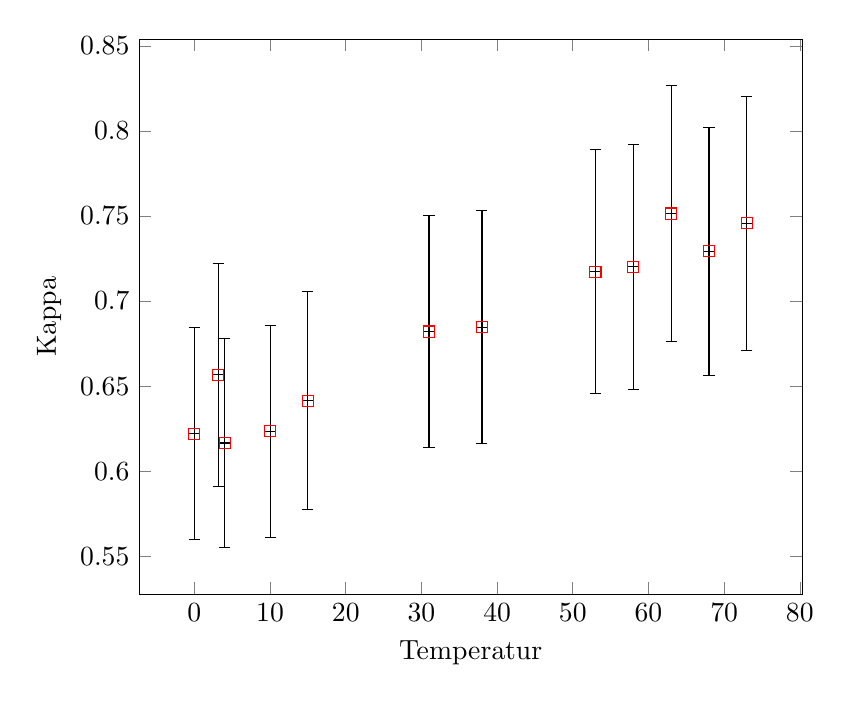
\begin{tikzpicture}
		\pgfplotsset{width=10cm,legend style={font=\footnotesize}}
		\begin{axis}[xlabel={Temperatur},ylabel={Kappa},legend cell align=left,legend pos=north west]
		\addplot+[only marks,color=red,mark=square,error bars/.cd,x dir=both,x explicit,y dir=both,y explicit,error bar style={color=black}] table[x=X,y=Y,x error=xerror,y error=yerror,row sep=\\]{
			X	Y	xerror	yerror	\\
			3.141592653589793	0.6565661435410208	0	0.06565661435410208	\\
			73	0.745651428687384	0	0.0745651428687384	\\
			68	0.7291896973891191	0	0.07291896973891192	\\
			63	0.7514142988993405	0	0.07514142988993405	\\
			58	0.7202039843396486	0	0.07202039843396486	\\
			53	0.7171452345550323	0	0.07171452345550323	\\
			38	0.6845595922438421	0	0.06845595922438422	\\
			31	0.682063770279751	0	0.06820637702797509	\\
			15	0.6413677738717087	0	0.06413677738717087	\\
			10	0.623492704217991	0	0.0623492704217991	\\
			4	0.6165815992240085	0	0.06165815992240085	\\
			0	0.622000108043746	0	0.062200010804374595	\\
		};		% \addlegendentry{Messpunkte Datensatz 0}
		\end{axis}
		\end{tikzpicture}
	\caption{$\kappa(T)$}
	\label{fig:KappaTemperatur}
\end{figure}
        The above figure shows the correlation between the isentropic exponent and the temperature. Qualitatively, we can see that the isentropic exponent is higher when the temperature is higher. This expected, as $\kappa=\frac{f+2}{f}$ and we have more effective degrees of freedom for higher temperaturs: or vice versa, the colder a substance is, the less energy it has to active all its degrees of freedom.\\

        \noindent Additionally, the figure shown below plots the degrees of freedom over the temperature. The behaviour here is much more chaotic and even displays some negative degrees of freedom. This ist most likely due to a yet undiscovered calculation error.

        \begin{figure}[H]
	\centering
	\begin{tikzpicture}
		\pgfplotsset{width=10cm,legend style={font=\footnotesize}}
		\begin{axis}[xlabel={Temperatur},ylabel={Freiheit},legend cell align=left,legend pos=north west]
		\addplot+[only marks,color=red,mark=square,error bars/.cd,x dir=both,x explicit,y dir=both,y explicit,error bar style={color=black}] table[x=X,y=Y,x error=xerror,y error=yerror,row sep=\\]{
			X	Y	xerror	yerror	\\
			3.141592653589793	-19.587152221267605	0	-1.9587152221267605	\\
			73	35.61118695932225	0	3.5611186959322247	\\
			68	-60.65178959028931	0	-6.065178959028931	\\
			63	4.697996134713314	0	0.4697996134713314	\\
			58	0.8484052762734677	0	0.08484052762734678	\\
			53	13.795175511942787	0	1.3795175511942788	\\
			38	-3.4407061579130485	0	-0.3440706157913049	\\
			31	27.950236316457676	0	2.7950236316457677	\\
			15	-13.68049659008453	0	-1.3680496590084532	\\
			10	-10.126471807847185	0	-1.0126471807847186	\\
			4	-9.352740465879492	0	-0.9352740465879492	\\
			0	-9.080536481984176	0	-0.9080536481984176	\\
		};		% \addlegendentry{Messpunkte Datensatz 0}
		\end{axis}
		\end{tikzpicture}
	\caption{$f(T)$}
	\label{fig:FreiheitTemperatur}
\end{figure}
        
        
\end{document}